%%%%%%%%%%%%%%%%%%%%%%%%%%%%%%%%%%%%%%%%%
% Classicthesis Typographic Thesis
% LaTeX Template
% Version 1.4 (1/1/16)
%
% This template has been downloaded from:
% http://www.LaTeXTemplates.com
%
% Original author:
% André Miede (http://www.miede.de) with commenting modifications by:
% Vel (vel@LaTeXTemplates.com)
%
% License:
% GNU General Public License (v2)
%
% General Tips:
% 1) Make sure to edit the classicthesis-config.file
% 2) New enumeration (A., B., C., etc in small caps): \begin{aenumerate} \end{aenumerate}
% 3) For margin notes: \marginpar or \graffito{}
% 4) Do not use bold fonts in this style, it is designed around them
% 5) Use tables as in the examples
% 6) See classicthesis-preamble.sty for useful commands
%
%%%%%%%%%%%%%%%%%%%%%%%%%%%%%%%%%%%%%%%%%

%----------------------------------------------------------------------------------------
%	PACKAGES AND OTHER DOCUMENT CONFIGURATIONS
%----------------------------------------------------------------------------------------

\documentclass[
		twoside,openright,titlepage,numbers=noenddot,headinclude,%1headlines,
	 	footinclude=true,cleardoublepage=empty,
		dottedtoc, % Make page numbers in the table of contents flushed right with dots leading to them
		BCOR=5mm,paper=a4,fontsize=11pt, % Binding correction, paper type and font size
		french,american, % Languages, change this to your language(s)
		]{scrreprt} 
                
% Includes the file which contains all the document configurations and packages - make sure to edit this file
%%%%%%%%%%%%%%%%%%%%%%%%%%%%%%%%%%%%%%%%%
% Classicthesis Typographic Thesis
% Configuration File
%
% This file has been downloaded from:
% http://www.LaTeXTemplates.com
%
% Original author:
% André Miede (http://www.miede.de) with extensive commenting changes by:
% Vel (vel@LaTeXTemplates.com)
%
% License:
% GNU General Public License (v2)
%
% Important note:
% The main lines to change in this file are in the DOCUMENT VARIABLES
% section, the rest of the file is for advanced configuration.
%
%%%%%%%%%%%%%%%%%%%%%%%%%%%%%%%%%%%%%%%%%

%----------------------------------------------------------------------------------------
%	CHARACTER ENCODING
%----------------------------------------------------------------------------------------

\PassOptionsToPackage{utf8}{inputenc} % Set the encoding of your files. UTF-8 is the only sensible encoding nowadays. If you can't read äöüßáéçèê∂åëæƒÏ€ then change the encoding setting in your editor, not the line below. If your editor does not support utf8 use another editor!
\usepackage{inputenc}

%----------------------------------------------------------------------------------------
%	DOCUMENT VARIABLES
%	Fill in the lines below to enter your information into the thesis template
%	Each of the commands can be cited anywhere in the thesis
%----------------------------------------------------------------------------------------

% Remove drafting to get rid of the '[ Date - classicthesis version 4.0 ]' text at the bottom of every page
\PassOptionsToPackage{eulerchapternumbers,listings,drafting, pdfspacing, subfig,beramono,eulermath,parts}{classicthesis}
% Available options: drafting parts nochapters linedheaders eulerchapternumbers beramono eulermath pdfspacing minionprospacing tocaligned dottedtoc manychapters listings floatperchapter subfig

\newcommand{\myTitle}{A Classic Thesis Style\xspace}
\newcommand{\mySubtitle}{An Homage to The Elements of Typographic Style\xspace}
\newcommand{\myDegree}{Doktor-Ingenieur (Dr.-Ing.)\xspace}
\newcommand{\myName}{André Miede\xspace}
\newcommand{\myProf}{Put name here\xspace}
\newcommand{\myOtherProf}{Put name here\xspace}
\newcommand{\mySupervisor}{Put name here\xspace}
\newcommand{\myFaculty}{Put data here\xspace}
\newcommand{\myDepartment}{Put data here\xspace}
\newcommand{\myUni}{Put data here\xspace}
\newcommand{\myLocation}{Saarbrücken\xspace}
\newcommand{\myTime}{September 2015\xspace}
\newcommand{\myVersion}{version 4.2\xspace}

%----------------------------------------------------------------------------------------
%	USEFUL COMMANDS
%----------------------------------------------------------------------------------------

\newcommand{\ie}{i.\,e.}
\newcommand{\Ie}{I.\,e.}
\newcommand{\eg}{e.\,g.}
\newcommand{\Eg}{E.\,g.} 

\newcounter{dummy} % Necessary for correct hyperlinks (to index, bib, etc.)
\providecommand{\mLyX}{L\kern-.1667em\lower.25em\hbox{Y}\kern-.125emX\@}
\newlength{\abcd} % for ab..z string length calculation

%----------------------------------------------------------------------------------------
%	PACKAGES
%----------------------------------------------------------------------------------------

\usepackage{lipsum} % Used for inserting dummy 'Lorem ipsum' text into the template

%------------------------------------------------

%\PassOptionsToPackage{ngerman,american}{babel}  % Change this to your language(s)
% Spanish languages need extra options in order to work with this template
%\PassOptionsToPackage{spanish,es-lcroman}{babel}
\usepackage{babel}

%------------------------------------------------			

\usepackage{csquotes}
\PassOptionsToPackage{%
%backend=biber, % Instead of bibtex
backend=bibtex8,bibencoding=ascii,%
language=auto,%
style=numeric-comp,%
%style=authoryear-comp, % Author 1999, 2010
%bibstyle=authoryear,dashed=false, % dashed: substitute rep. author with ---
sorting=nyt, % name, year, title
maxbibnames=10, % default: 3, et al.
%backref=true,%
natbib=true % natbib compatibility mode (\citep and \citet still work)
}{biblatex}
\usepackage{biblatex}
 
 %------------------------------------------------

\PassOptionsToPackage{fleqn}{amsmath} % Math environments and more by the AMS 
 \usepackage{amsmath}
 
 %------------------------------------------------

\PassOptionsToPackage{T1}{fontenc} % T2A for cyrillics
\usepackage{fontenc}

%------------------------------------------------

\usepackage{textcomp} % Fix warning with missing font shapes

%------------------------------------------------

\usepackage{scrhack} % Fix warnings when using KOMA with listings package  

%------------------------------------------------

\usepackage{xspace} % To get the spacing after macros right

%------------------------------------------------

\usepackage{mparhack} % To get marginpar right

%------------------------------------------------

\usepackage{fixltx2e} % Fixes some LaTeX stuff 

%------------------------------------------------

\PassOptionsToPackage{smaller}{acronym} % Include printonlyused in the first bracket to only show acronyms used in the text
\usepackage{acronym} % Nice macros for handling all acronyms in the thesis

%\renewcommand*{\acsfont}[1]{\textssc{#1}} % For MinionPro
\renewcommand*{\aclabelfont}[1]{\acsfont{#1}}

%------------------------------------------------

\PassOptionsToPackage{pdftex}{graphicx}
\usepackage{graphicx} 

%----------------------------------------------------------------------------------------
%	FLOATS: TABLES, FIGURES AND CAPTIONS SETUP
%----------------------------------------------------------------------------------------

\usepackage{tabularx} % Better tables
\setlength{\extrarowheight}{3pt} % Increase table row height
\newcommand{\tableheadline}[1]{\multicolumn{1}{c}{\spacedlowsmallcaps{#1}}}
\newcommand{\myfloatalign}{\centering} % To be used with each float for alignment
\usepackage{caption}
\captionsetup{font=small}
\usepackage{subfig}  

%----------------------------------------------------------------------------------------
%	CODE LISTINGS SETUP
%----------------------------------------------------------------------------------------

\usepackage{listings} 
%\lstset{emph={trueIndex,root},emphstyle=\color{BlueViolet}}%\underbar} % For special keywords
\lstset{language=[LaTeX]Tex,%C++ % Specify the language(s) for listings here
morekeywords={PassOptionsToPackage,selectlanguage},
keywordstyle=\color{RoyalBlue}, % Add \bfseries for bold
basicstyle=\small\ttfamily, % Makes listings a smaller font size and a different font
%identifierstyle=\color{NavyBlue}, % Color of text inside brackets
commentstyle=\color{Green}\ttfamily, % Color of comments
stringstyle=\rmfamily, % Font type to use for strings
numbers=left, % Change left to none to remove line numbers
numberstyle=\scriptsize, % Font size of the line numbers
stepnumber=5, % Increment of line numbers
numbersep=8pt, % Distance of line numbers from code listing
showstringspaces=false, % Sets whether spaces in strings should appear underlined
breaklines=true, % Force the code to stay in the confines of the listing box
%frameround=ftff, % Uncomment for rounded frame
%frame=single, % Frame border - none/leftline/topline/bottomline/lines/single/shadowbox/L
belowcaptionskip=.75\baselineskip % Space after the "Listing #: Desciption" text and the listing box
}

%----------------------------------------------------------------------------------------
%	HYPERREFERENCES
%----------------------------------------------------------------------------------------

\PassOptionsToPackage{pdftex,hyperfootnotes=false,pdfpagelabels}{hyperref}
\usepackage{hyperref}  % backref linktocpage pagebackref
\pdfcompresslevel=9
\pdfadjustspacing=1

\hypersetup{
% Uncomment the line below to remove all links (to references, figures, tables, etc), useful for b/w printouts
%draft, 
colorlinks=true, linktocpage=true, pdfstartpage=3, pdfstartview=FitV,
% Uncomment the line below if you want to have black links (e.g. for printing black and white)
%colorlinks=false, linktocpage=false, pdfborder={0 0 0}, pdfstartpage=3, pdfstartview=FitV, 
breaklinks=true, pdfpagemode=UseNone, pageanchor=true, pdfpagemode=UseOutlines,%
plainpages=false, bookmarksnumbered, bookmarksopen=true, bookmarksopenlevel=1,%
hypertexnames=true, pdfhighlight=/O,%nesting=true,%frenchlinks,%
urlcolor=webbrown, linkcolor=RoyalBlue, citecolor=webgreen, %pagecolor=RoyalBlue,%
    %urlcolor=Black, linkcolor=Black, citecolor=Black, %pagecolor=Black,%
%------------------------------------------------
% PDF file meta-information
pdftitle={\myTitle},
pdfauthor={\textcopyright\ \myName, \myUni, \myFaculty},
pdfsubject={},
pdfkeywords={},
pdfcreator={pdfLaTeX},
pdfproducer={LaTeX with hyperref and classicthesis}
%------------------------------------------------
}

%----------------------------------------------------------------------------------------
%	AUTOREFERENCES SETUP
%	Redefines how references in text are prefaced for different 
%	languages (e.g. "Section 1.2" or "section 1.2")
%----------------------------------------------------------------------------------------

\makeatletter
\@ifpackageloaded{babel}
{
\addto\extrasamerican{
\renewcommand*{\figureautorefname}{Figure}
\renewcommand*{\tableautorefname}{Table}
\renewcommand*{\partautorefname}{Part}
\renewcommand*{\chapterautorefname}{Chapter}
\renewcommand*{\sectionautorefname}{Section}
\renewcommand*{\subsectionautorefname}{Section}
\renewcommand*{\subsubsectionautorefname}{Section}
}
\addto\extrasngerman{
\renewcommand*{\paragraphautorefname}{Absatz}
\renewcommand*{\subparagraphautorefname}{Unterabsatz}
\renewcommand*{\footnoteautorefname}{Fu\"snote}
\renewcommand*{\FancyVerbLineautorefname}{Zeile}
\renewcommand*{\theoremautorefname}{Theorem}
\renewcommand*{\appendixautorefname}{Anhang}
\renewcommand*{\equationautorefname}{Gleichung}
\renewcommand*{\itemautorefname}{Punkt}
}
\providecommand{\subfigureautorefname}{\figureautorefname} % Fix to getting autorefs for subfigures right
}{\relax}
\makeatother

%----------------------------------------------------------------------------------------

\usepackage{classicthesis} 

%----------------------------------------------------------------------------------------
%	CHANGING TEXT AREA 
%----------------------------------------------------------------------------------------

%\linespread{1.05} % a bit more for Palatino
%\areaset[current]{312pt}{761pt} % 686 (factor 2.2) + 33 head + 42 head \the\footskip
%\setlength{\marginparwidth}{7em}%
%\setlength{\marginparsep}{2em}%

%----------------------------------------------------------------------------------------
%	USING DIFFERENT FONTS
%----------------------------------------------------------------------------------------

%\usepackage[oldstylenums]{kpfonts} % oldstyle notextcomp
%\usepackage[osf]{libertine}
%\usepackage[light,condensed,math]{iwona}
%\renewcommand{\sfdefault}{iwona}
%\usepackage{lmodern} % <-- no osf support :-(
%\usepackage{cfr-lm} % 
%\usepackage[urw-garamond]{mathdesign} <-- no osf support :-(
%\usepackage[default,osfigures]{opensans} % scale=0.95 
%\usepackage[sfdefault]{FiraSans}

%%%%%%%%%
% biblio
\addbibresource{/Users/Juste/Documents/ComplexSystems/CityNetwork/Biblio/Bibtex/CityNetwork.bib} % The file housing your bibliography
%\addbibresource[label=ownpubs]{Self_Publications.bib} % Uncomment for optional self-publications
\addbibresource{Biblio/transportationEquilibrium.bib}
\addbibresource{Biblio/robustnessDiscrepancy.bib}
\addbibresource{Biblio/syntheticData.bib}


%%%%%
%% Language 0 for english ; 1 for french
%\def \thelanguage {0}
\def \thelanguage {1}

%%%%%
% variable to include comments or not in the compilation ; set to 1 to include
\def \draft {1}
%\def \draft {0}



% customized header
%% Commands

\newcommand{\noun}[1]{\textsc{#1}}

% command fort head of chapter citation
\newcommand{\headercit}[3]{
\begin{multicols}{2}
\phantom{}
\columnbreak
\textit{#1}

 - \noun{#2}~#3
\end{multicols}
}



%% Math

% Operators
\DeclareMathOperator{\Cov}{Cov}
\DeclareMathOperator{\Var}{Var}
\DeclareMathOperator{\E}{\mathbb{E}}
\DeclareMathOperator{\Proba}{\mathbb{P}}

\newcommand{\Covb}[2]{\ensuremath{\Cov\!\left[#1,#2\right]}}
\newcommand{\Eb}[1]{\ensuremath{\E\!\left[#1\right]}}
\newcommand{\Pb}[1]{\ensuremath{\Proba\!\left[#1\right]}}
\newcommand{\Varb}[1]{\ensuremath{\Var\!\left[#1\right]}}

% norm
\newcommand{\norm}[1]{\| #1 \|}

% independent
\newcommand{\indep}{\rotatebox[origin=c]{90}{$\models$}}


% amsthm environments
\newtheorem{definition}{Definition}
\newtheorem{proposition}{Proposition}
\newtheorem{assumption}{Assumption}
\newtheorem{lemma}{Lemma}

\newenvironment{proof}[1][Proof]{\begin{trivlist}
\item[\hskip \labelsep {\bfseries #1}]}{\end{trivlist}}




\newcommand{\qed}{\nobreak \ifvmode \relax \else
      \ifdim\lastskip<1.5em \hskip-\lastskip
      \hskip1.5em plus0em minus0.5em \fi \nobreak
      \vrule height0.75em width0.5em depth0.25em\fi}



%%%%%%%%%%%%%%%%%%%
%%  Additional packages
%%%%%%%%%%%%%%%%%%%

%\usepackage{subcaption}

\usepackage{amssymb}

\usepackage{multicol}

\usepackage{bbm}

% chinese
%\usepackage{ctex}
%\setCJKmainfont[BoldFont=FandolSong-Bold.otf,ItalicFont=FandolKai-Regular.otf]{FandolSong-Regular.otf}
%\setCJKsansfont[BoldFont=FandolHei-Bold.otf]{FandolHei-Regular.otf}
%\setCJKmonofont{FandolFang-Regular.otf}

%  --> needs XeLateX ? then needs to comment pdflatex options in class definition.

\usepackage{mdframed}

%%%

\renewcommand{\PrelimText}{%
  \footnotesize[\,\today\ at \thistime\ -- \texttt{Thesis}~\myVersion\,]}


%%%%%%%%
% bilingual version
\usepackage{xparse}
\usepackage{ifthen}


% biling paragraph

\newcommand{\bpar}[2]{
    \ifthenelse{\thelanguage=0}{#1}{}
    \ifthenelse{\thelanguage=1}{#2}{}
}


% Sectioning commands
% from http://tex.stackexchange.com/questions/109557/renewdefine-section-with-additional-argument


%\let\oldchapter\chapter
%
%\RenewDocumentCommand\chapter {s o o m m}
%   {
%    \IfBooleanTF{#1}                   
%        {
%        \ifthenelse{\thelanguage=0}{\oldchapter*{#4}}{}
%        \ifthenelse{\thelanguage=1}{\oldchapter*{#5}}{}
%          \IfNoValueF{#2}            % if TOC arg is given create a TOC entry
%            {          
%              \ifthenelse{\thelanguage=0}{\addcontentsline{toc}{chapter}{#2}}{}
%              \ifthenelse{\thelanguage=1}{\addcontentsline{toc}{chapter}{#3}}{}
%            }
%        }  
%      {                              % no star given 
%        \IfNoValueTF{#2}
%          {
%            \ifthenelse{\thelanguage=0}{\oldchapter{#4}}{}
%            \ifthenelse{\thelanguage=1}{\oldchapter{#5}}{}
%           }       % no TOC arg
%          { 
%            \ifthenelse{\thelanguage=0}{\oldchapter[#2]{#4}}{}
%            \ifthenelse{\thelanguage=1}{\oldchapter[#3]{#5}}{}
%           }
%      }   
%  }
%
%



\let\oldsection\section

\RenewDocumentCommand\section {s o o m m}
   {
    \IfBooleanTF{#1}                   
        {
        \ifthenelse{\thelanguage=0}{\oldsection*{#4}}{}
        \ifthenelse{\thelanguage=1}{\oldsection*{#5}}{}
          \IfNoValueF{#2}            % if TOC arg is given create a TOC entry
            {          
              \ifthenelse{\thelanguage=0}{\addcontentsline{toc}{section}{#2}}{}
              \ifthenelse{\thelanguage=1}{\addcontentsline{toc}{section}{#3}}{}
            }
        }  
      {                              % no star given 
        \IfNoValueTF{#2}
          {
            \ifthenelse{\thelanguage=0}{\oldsection{#4}}{}
            \ifthenelse{\thelanguage=1}{\oldsection{#5}}{}
           }       % no TOC arg
          { 
            \ifthenelse{\thelanguage=0}{\oldsection[#2]{#4}}{}
            \ifthenelse{\thelanguage=1}{\oldsection[#3]{#5}}{}
           }
      }   
  }

\let\oldsubsection\subsection

\RenewDocumentCommand\subsection {s o o m m}
   {
    \IfBooleanTF{#1}                   
        {
        \ifthenelse{\thelanguage=0}{\oldsubsection*{#4}}{}
        \ifthenelse{\thelanguage=1}{\oldsubsection*{#5}}{}
          \IfNoValueF{#2}            % if TOC arg is given create a TOC entry
             {          
              \ifthenelse{\thelanguage=0}{\addcontentsline{toc}{subsection}{#2}}{}
              \ifthenelse{\thelanguage=1}{\addcontentsline{toc}{subsection}{#3}}{}
            }
        }  
      {                              % no star given 
        \IfNoValueTF{#2}
          {
           \ifthenelse{\thelanguage=0}{\oldsubsection{#4}}{}
           \ifthenelse{\thelanguage=1}{\oldsubsection{#5}}{}
           }       % no TOC arg
          { 
           \ifthenelse{\thelanguage=0}{\oldsubsection[#2]{#4}}{}
           \ifthenelse{\thelanguage=1}{\oldsubsection[#3]{#5}}{}
           }
      }   
  }


\let\oldsubsubsection\subsubsection

\RenewDocumentCommand\subsubsection {s o o m m}
   {
    \IfBooleanTF{#1}   
        {
        \ifthenelse{\thelanguage=0}{\oldsubsubsection*{#4}}{}
        \ifthenelse{\thelanguage=1}{\oldsubsubsection*{#5}}{}
          \IfNoValueF{#2}            % if TOC arg is given create a TOC entry
             {          
              \ifthenelse{\thelanguage=0}{\addcontentsline{toc}{subsubsection}{#2}}{}
              \ifthenelse{\thelanguage=1}{\addcontentsline{toc}{subsubsection}{#3}}{}
            }
        }  
      {                              % no star given 
        \IfNoValueTF{#2}
          {
           \ifthenelse{\thelanguage=0}{\oldsubsubsection{#4}}{}
           \ifthenelse{\thelanguage=1}{\oldsubsubsection{#5}}{}
           }       % no TOC arg
          { 
           \ifthenelse{\thelanguage=0}{\oldsubsubsection[#2]{#4}}{}
           \ifthenelse{\thelanguage=1}{\oldsubsubsection[#3]{#5}}{}
           }
      }   
  }
  
  
  
\let\oldparagraph\paragraph

\RenewDocumentCommand\paragraph {s m m}
   {
    \IfBooleanTF{#1}
        {
        \ifthenelse{\thelanguage=0}{\oldparagraph*{#2}}{}
        \ifthenelse{\thelanguage=1}{\oldparagraph*{#3}}{}
        }  
      { 
           \ifthenelse{\thelanguage=0}{\oldparagraph{#2}}{}
           \ifthenelse{\thelanguage=1}{\oldparagraph{#3}}{}   
      }   
  }


\let\oldcaption\caption

\RenewDocumentCommand\caption {o o m m}
   {
        \IfNoValueTF{#1}
          {
           \ifthenelse{\thelanguage=0}{\oldcaption{#3}}{}
           \ifthenelse{\thelanguage=1}{\oldcaption{#4}}{}
           }       % no TOC arg
          { 
           \ifthenelse{\thelanguage=0}{\oldcaption[#1]{#3}}{}
           \ifthenelse{\thelanguage=1}{\oldcaption[#2]{#4}}{}
           }
      } 
      
      
        
%%%%%%%%%%
%  Citation

\let\oldcite\cite
\renewcommand{\cite}[1]{[\oldcite{#1}]}




%%%%%%%%%%
%  Drafting

% writing utilities

% comments	 and responses
%  -> use this comment to ask questions on what other wrote/answer questions with optional arguments (up to 4 answers)


\DeclareDocumentCommand{\comment}{m o o o o}
{\ifthenelse{\draft=1}{
    \textcolor{red}{\textbf{C : }#1}
    \IfValueT{#2}{\textcolor{blue}{\textbf{A1 : }#2}}
    \IfValueT{#3}{\textcolor{ForestGreen}{\textbf{A2 : }#3}}
    \IfValueT{#4}{\textcolor{red!50!blue}{\textbf{A3 : }#4}}
    \IfValueT{#5}{\textcolor{Aquamarine}{\textbf{A4 : }#5}}
 }{}
}


% todo
\newcommand{\todo}[1]{
    \ifthenelse{\draft=1}{\textcolor{red!50!blue}{\textbf{TODO : \textit{#1}}}}{}
}



% provisory part, removed if not draft


\newcommand{\provisory}[1]{
    \ifthenelse{\draft=1}{
    \color{blue} \textbf{\textit{PROVISORY}} #1 \color{black}
    }{}
}

%\newenvironment{provisory}{\par\color{blue}}{\par}












% BUG FIX for biblio (biblatex)
% see http://tex.stackexchange.com/questions/311426/bibliography-error-use-of-blxbblverbaddi-doesnt-match-its-definition-ve
\makeatletter
\def\blx@maxline{77}
\makeatother





%\hyphenation{Put special hyphenation here}

\begin{document}

\frenchspacing % Reduces space after periods to make text more compact

\raggedbottom % Makes all pages the height of the text on that page

\ifthenelse{\thelanguage=0}{\selectlanguage{american}}{\selectlanguage{french}}
% Select your default language - e.g. american or ngerman

%\renewcommand*{\bibname}{new name} % Uncomment to change the name of the bibliography
%\setbibpreamble{} % Uncomment to include a preamble to the bibliography - some text before the reference list starts

\pagenumbering{roman} % Roman page numbering prior to the start of the thesis content (i, ii, iii, etc)

\pagestyle{plain} % Suppress headers for the pre-content pages


%----------------------------------------------------------------------------------------
%	PRE-CONTENT THESIS PAGES
%----------------------------------------------------------------------------------------

% Title Page

\begin{titlepage}

\begin{addmargin}[-1cm]{-3cm}
\begin{center}
\large

\hfill
\vfill

\begingroup
\color{Maroon}\spacedallcaps{\myTitle} \\ \bigskip % Thesis title
\endgroup

\spacedlowsmallcaps{\myName} % Your name

\vfill

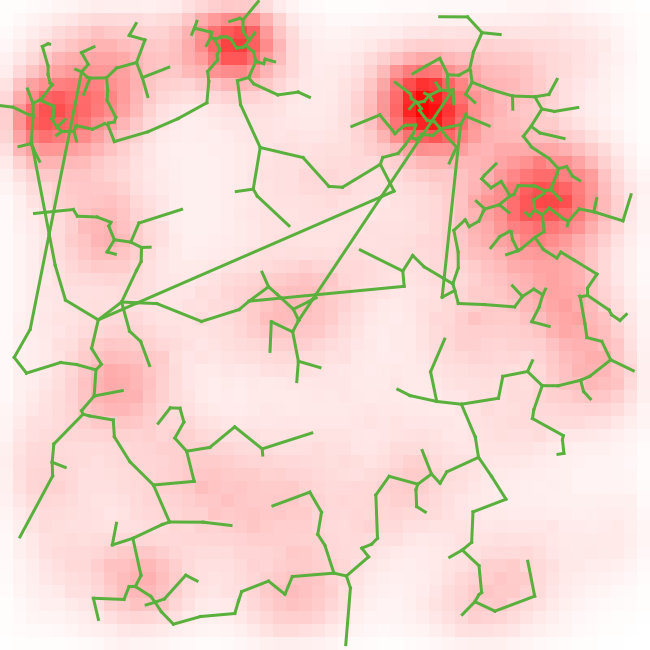
\includegraphics[width=\textwidth]{Figures/Cover/cover} \\ \vspace{3cm} % Picture

\mySubtitle \\ \medskip % Thesis subtitle
Under the supervision of \myProf and \myOtherProf \\ \medskip
%\myDegree \\
\myDepartment \\  \medskip
\myFaculty \\  \bigskip
%\myUni \\ \bigskip

\myTime\ -- \myVersion % Time and version

\vfill

\end{center}
\end{addmargin}

\end{titlepage} % Main title page

% Back of the title page

\thispagestyle{empty}

\hfill

\vfill

\noindent\myName: \textit{\myTitle,} \mySubtitle, %\myDegree, 
\textcopyright\ \myTime

% You may wish to do something with the back of the title page, such as including your supervisors, location or time frame of the work. Below is an example of doing so although you may want to tweak it to your liking.

%\bigskip

%\noindent\spacedlowsmallcaps{Supervisors}: \\
%\myProf \\
%\myOtherProf \\ 
%\mySupervisor

%\medskip \\

%\noindent\spacedlowsmallcaps{Location}: \\
%\myLocation

%\medskip \\

%\noindent\spacedlowsmallcaps{Time Frame}: \\
%\myTime
 % Back of the title page

\cleardoublepage% Dedication

\thispagestyle{empty}
\refstepcounter{dummy}

\pdfbookmark[1]{Dedication}{Dedication} % Bookmark name visible in a PDF viewer

\vspace*{3cm}

\begin{center}
\emph{Ohana} means family. \\
Family means nobody gets left behind, or forgotten. \\ \medskip
--- Lilo \& Stitch    
\end{center}

\medskip

\begin{center}
Dedicated to the loving memory of Rudolf Miede. \\ \smallskip
1939\,--\,2005
\end{center} % Dedication page

\cleardoublepage% Abstract

%\renewcommand{\abstractname}{Abstract} % Uncomment to change the name of the abstract

\pdfbookmark[1]{Abstract}{Abstract} % Bookmark name visible in a PDF viewer

\begingroup
\let\clearpage\relax
\let\cleardoublepage\relax
\let\cleardoublepage\relax

\chapter*{Abstract}
%Short summary of the contents\dots a great guide by 
%Kent Beck how to write good abstracts can be found here:  
%\begin{center}
%\url{https://plg.uwaterloo.ca/~migod/research/beckOOPSLA.html}
%\end{center}









\endgroup			

\vfill % Abstract page



\cleardoublepage
% Abstract

%\renewcommand{\abstractname}{Abstract} % Uncomment to change the name of the abstract

\pdfbookmark[1]{Reading Notes}{Reading Notes} % Bookmark name visible in a PDF viewer

\begingroup
\let\clearpage\relax
\let\cleardoublepage\relax
\let\cleardoublepage\relax

\chapter*{Reading Notes}{Notes de Lecture}

\textit{This provisory Memoire must be read as a work in progress, as it details progresses after one year of Doctorate. Many parts are given at the state of project, and not omitted as playing a role in the current research questioning. Its purpose is to set up a plan and examine the achieved work and corresponding directions, but also to share research ideas at this important step of one year.}




\endgroup			

\vfill



 % Uncomment and create a Foreword.tex to include a foreword



\cleardoublepage% Publications - a page listing research articles written using content in the thesis

\pdfbookmark[1]{Publications}{Publications} % Bookmark name visible in a PDF viewer

\chapter*{Publications}{Publications} % Publications page text

%Some ideas and figures have appeared previously in the following publications:\\

%\noindent Put your publications from the thesis here. The packages \texttt{multibib} or \texttt{bibtopic} etc. can be used to handle multiple different bibliographies in your document.

%\begin{refsection}[ownpubs]
%    \small
%    \nocite{*} % is local to to the enclosing refsection
%    \printbibliography[heading=none]
%\end{refsection}

%\emph{Attention}: This requires a separate run of \texttt{bibtex} for your \texttt{refsection}, \eg, \texttt{ClassicThesis1-blx} for this file. You might also use \texttt{biber} as the backend for \texttt{biblatex}. See also \url{http://tex.stackexchange.com/questions/128196/problem-with-refsection}.

\bpar{
The following works have an highly overlapping content with this thesis:
}{
Les travaux suivants contiennent une grande partie du contenu de cette thèse:
}

% NOTE : on self-plagiarism, be careful to precise when extract from a published paper : 
%  - http://academia.stackexchange.com/questions/12342/self-plagiarism-in-phd-thesis
%  - http://academia.stackexchange.com/questions/2029/can-i-use-the-work-in-my-journal-conference-publications-as-chapters-in-my-disse
%  - http://academia.stackexchange.com/questions/149/what-is-a-sandwich-thesis


\section*{Publications}{Publications}


\noindent Antelope, C., Hubatsch, L., Raimbault, J., and Serna, J. M. (2016). An interdisciplinary approach to morphogenesis. Forthcoming in Proceedings of Santa Fe Institute CSSS 2016.


\bigskip

\noindent Raimbault, J. (2017). A Discrepancy-Based Framework to Compare Robustness Between Multi-attribute Evaluations. In Complex Systems Design \& Management (pp. 141-154). Springer International Publishing.

\bigskip

\noindent Raimbault, J. (2016). Investigating the Empirical Existence of Static User Equilibrium, \textit{forthcoming in EWGT 2016 proceedings, Transportation Research Procedia.} arxiv:1608.05266


\bigskip


\noindent Raimbault, J. (2016). Generation of Correlated Synthetic Data, forthcoming in \textit{Actes des Journ{\'e}es de Rochebrune 2016.}


\bigskip

\noindent Raimbault, J. (2015). Models Coupling Urban Growth and Transportation Network Growth: An Algorithmic Systematic Review Approach, forthcoming in \textit{ECTQG 2015 proceedings.} arxiv:1605.08888


\section*{Communications}{Communications}

\noindent Towards a Theory of Co-evolutive Networked Territorial Systems: Insights from Transportation Governance Modeling in Pearl River Delta, China, \textit{MEDIUM Seminar : Sustainable Development in Zhuhai, Guangzhou, Dec 2016.}


\bigskip


\noindent Models of growth for system of cities : Back to the simple, \textit{Conference on Complex Systems 2016, Amsterdam, Sep 2016.}



%Raimbault J., Bergeaud A. and Potiron Y. (2016). Investigating Patterns of Technological Innovation. \textit{Conference on Complex Systems 2016, Amsterdam, Sep 2016.}


\bigskip

\noindent For a Cautious Use of Big Data and Computation. \textit{Royal Geographical Society - Annual Conference 2016 - Session : Geocomputation, the Next 20 Years (1), London, Aug 2016.}


\bigskip

\noindent Indirect Bibliometrics by Complex Network Analysis. \textit{20e Anniversaire de Cybergeo, Paris, May 2016.}


\bigskip

\noindent Raimbault, J. \& Serra, H. (2016). Game-based Tools as Media to Transmit Freshwater Ecology Concepts, \textit{poster corner at SETAC 2016 (Nantes, May 2016).}


\bigskip

\noindent Le Néchet, F. \& Raimbault, J. (2015). Modeling the emergence of metropolitan transport authority in a polycentric urban region, \textit{ECTQG 2015, Bari, Sep 2015).}


\bigskip

\noindent Hybrid Modeling of a Bike-Sharing Transportation System, \textit{poster presented at ICCSS 2015, Helsinki, June 2015.}

\bigskip

\noindent Raimbault, J. \& Gonzales, J. (2015). Application de la Morphog{\'e}n{\`e}se de R{\'e}seaux Biologiques {\`a} la Conception Optimale d'Infrastructures de Transport, \textit{poster presented at Rencontres du Labex Dynamite, Paris, May 2015.}


 % Publications from the thesis page

%\cleardoublepage% Acknowledgements

\pdfbookmark[1]{Acknowledgements}{Acknowledgements} % Bookmark name visible in a PDF viewer

\begin{flushright}{\slshape    
We have seen that computer programming is an art, \\ 
because it applies accumulated knowledge to the world, \\ 
because it requires skill and ingenuity, and especially \\
because it produces objects of beauty.} \\ \medskip
--- \defcitealias{knuth:1974}{Donald E. Knuth}\citetalias{knuth:1974} \citep{knuth:1974}
\end{flushright}

\bigskip

%----------------------------------------------------------------------------------------

\begingroup

\let\clearpage\relax
\let\cleardoublepage\relax
\let\cleardoublepage\relax

\chapter*{Acknowledgements}

\noindent Put your acknowledgements here.\\

\noindent Many thanks to everybody who already sent me a postcard!\\

\noindent Regarding the typography and other help, many thanks go to Marco Kuhlmann, Philipp Lehman, Lothar Schlesier, Jim Young, Lorenzo Pantieri and Enrico Gregorio\footnote{Members of GuIT (Gruppo Italiano Utilizzatori di \TeX\ e \LaTeX )}, J\"org Sommer, Joachim K\"ostler, Daniel Gottschlag, Denis Aydin, Paride Legovini, Steffen Prochnow, Nicolas Repp, Hinrich Harms, Roland Winkler, and the whole \LaTeX-community for support, ideas and some great software.

\bigskip

\noindent\emph{Regarding \mLyX}: The \mLyX\ port was initially done by
\emph{Nicholas Mariette} in March 2009 and continued by
\emph{Ivo Pletikosi\'c} in 2011. Thank you very much for your work and the contributions to the original style.

\endgroup % Acknowledgements page

\pagestyle{scrheadings} % Show chapter titles as headings

\cleardoublepage% Table of Contents - List of Tables/Figures/Listings and Acronyms

\refstepcounter{dummy}

\pdfbookmark[1]{\contentsname}{tableofcontents} % Bookmark name visible in a PDF viewer

\setcounter{tocdepth}{1} % Depth of sections to include in the table of contents - currently up to subsections

\setcounter{secnumdepth}{2} % Depth of sections to number in the text itself - currently up to subsubsections

\manualmark
\markboth{\spacedlowsmallcaps{\contentsname}}{\spacedlowsmallcaps{\contentsname}}
\tableofcontents 
\automark[section]{chapter}
\renewcommand{\chaptermark}[1]{\markboth{\spacedlowsmallcaps{#1}}{\spacedlowsmallcaps{#1}}}
\renewcommand{\sectionmark}[1]{\markright{\thesection\enspace\spacedlowsmallcaps{#1}}}

\clearpage

\begingroup 
\let\clearpage\relax
\let\cleardoublepage\relax
\let\cleardoublepage\relax

%----------------------------------------------------------------------------------------
%	List of Figures
%----------------------------------------------------------------------------------------

\refstepcounter{dummy}
%\addcontentsline{toc}{chapter}{\listfigurename} % Uncomment if you would like the list of figures to appear in the table of contents
\pdfbookmark[1]{\listfigurename}{lof} % Bookmark name visible in a PDF viewer

\listoffigures

\vspace{8ex}
%\newpage

%----------------------------------------------------------------------------------------
%	List of Tables
%----------------------------------------------------------------------------------------

\refstepcounter{dummy}
%\addcontentsline{toc}{chapter}{\listtablename} % Uncomment if you would like the list of tables to appear in the table of contents
\pdfbookmark[1]{\listtablename}{lot} % Bookmark name visible in a PDF viewer

%\chapter*{List of Tables}

\phantomsection

\listoftables
        
\vspace{8ex}
\newpage
    
%----------------------------------------------------------------------------------------
%	List of Listings
%---------------------------------------------------------------------------------------- 

%\refstepcounter{dummy}
%\addcontentsline{toc}{chapter}{\lstlistlistingname} % Uncomment if you would like the list of listings to appear in the table of contents
%\pdfbookmark[1]{\lstlistlistingname}{lol} % Bookmark name visible in a PDF viewer

%\lstlistoflistings 

%\vspace{8ex}
%\newpage
       
%----------------------------------------------------------------------------------------
%	Acronyms
%----------------------------------------------------------------------------------------

%\refstepcounter{dummy}
%\addcontentsline{toc}{chapter}{Acronyms} % Uncomment if you would like the acronyms to appear in the table of contents
%\pdfbookmark[1]{Acronyms}{acronyms} % Bookmark name visible in a PDF viewer

%\markboth{\spacedlowsmallcaps{Acronyms}}{\spacedlowsmallcaps{Acronyms}}

%\chapter*{Acronyms}

%\begin{acronym}[ABM]
%\acro{ABM}{Agent-based Modeling}
%\acro{API}{Application Programming Interface}
%\acro{UML}{Unified Modeling Language}
%\end{acronym}  
             
             

%\begin{acronym}[SOC]
%\acro{ABM}{Self-organized Criticality}
%\end{acronym} 
             
             
             
                   
\endgroup % Contents, list of figures/tables/listings and acronyms

\cleardoublepage

\pagenumbering{arabic} % Arabic page numbering for thesis content (1, 2, 3, etc)
%\setcounter{page}{90} % Uncomment to manually start the page counter at an arbitrary value (for example if you wish to count the pre-content pages in the page count)

\cleardoublepage % Avoids problems with pdfbookmark

%----------------------------------------------------------------------------------------
%	THESIS CONTENT - CHAPTERS
%----------------------------------------------------------------------------------------



%\ctparttext{}




%%% Test of translation to estimate translation speed %%%



\chapter*{Introduction}

% to have header for non-numbered introduction
\markboth{Introduction}{Introduction}

%\headercit{We need to find Banos' tenth modeling law}{Ren{\'e} Doursat}{}
\headercit{C'est quand on donne un coup de pied dans la fourmilière qu'on se rend compte de toute sa complexité.}{Arnaud Banos}{}

\bigskip

``En conséquence d'un problème technique, le trafic est interrompu sur la ligne B du RER pour une durée indéterminée. Plus d'information seront fournies dès que possible''. Il y a des fortes chances pour que quiconque ayant vécu ou passé un peu de temps en région parisienne ait déjà entendu cette annonce glaçante et en ait subi les conséquences pour le reste de la journée. Mais il ne se doute sûrement pas des ramifications des cascades causales induites par cet évènement presque banal. Les systèmes territoriaux, quelles que soient les aspects considérés pour leur définition, seront toujours extrêmement complexes, les interrelations à de nombreuses échelles spatiales et temporelles participant à la production des comportements émergents observés à tout niveau du système. Martin est un étudiant qui fait l'aller-retour journalier entre Paris et Palaiseau and manquera un examen crucial, ce qui aura un impact profond sur sa vie professionnelle : implications à une longue échelle de temps, une petite échelle spatiale et à la granularité de l'agent. Yuangsi était en train de relier les aéroports d'Orly et Roissy dans son voyage de Londres à Pékin et va manquer son avion ainsi que le mariage de sa soeur : grande échelle spatiale, petite échelle de temps, granularité de l'agent. Une pétition collective émerge des voyageurs, conduisant à la création d'une organisation qui mettra la pression sur les autorités pour qu'elles augmentent le niveau de service : échelle temporelle et spatiales mesoscopique, granularité de l'aggregation d'agents. La recherche de cause possible à l'incident conduira à des processus intriqués à diverses échelles, parmi lesquels aucun ne semble être une meilleure explication ; le développement historique du réseau ferroviaire en région parisienne a conditionné les écolutions futures et le RER B a suivi l'ancienne Ligne de Sceaux, le plan de \noun{Delouvrier} pour le développement régional et son execution partielle, sont également des éléments d'explication des faiblesses structurelles du réseau parisien de transports en commun~\cite{gleyze2005vulnerabilite} ; le motifs pendulaires dus à l'organisation territoriale induisent une surcharge de certaines ligne et ainsi nécessairement une augmentation des incidents d'exploitation. La liste pourrait être ainsi continuée un certain temps, chaque approche apportant sa vision mature correspondant à un corpus de connaissances scientifiques dans des disciplines diverses comme la géographie, l'économie urbains, les transports. Cette anecdote amusante est suffisante pour faire ressentir la complexité des systèmes territoriaux. Notre but ici est de se plonger dans cette complexité, et en particulier donner un point de vue original sur l'étude des relations entre réseaux et territoires. Le choix de cette position sera largement discuté dans une partie thématique, nous nous concentrons à présent sur l'originalité du point de vue que nous allons prendre.



%-------------------------------------------------

\section*{Contexte Scientifique : Paradigmes de la Complexité}

Pour une meilleure introduction du sujet, il est nécessaire d'insister sur le cadre scientifique dans lequel nous nous positionnons. Ce contexte est crucial à la fois pour comprendre les concepts épistémologiques implicites dans nos questions de recherche, et aussi pour être conscient de la variété de méthodes et outils utilisés. La science contemporaine prend progressivement le tournant de la complexité dans de nombreux champs, ce qui implique une mutation épistémologique pour abandonner le réductionnisme strict qui a échoué dans la majorité de ses tentatives de synthèse~\cite{anderson1972more}. Arthur a rappelé récemment~\cite{arthur2015complexity} qu'une mutation des méthodes et paradigmes en était également un enjeu, de par la place grandissante prise par les approches computationnelles qui remplacent les résolutions purement analytiques généralement limité en possibilités de modélisation et de résolution. La capture des \emph{propriétés émergentes} par des modèles de systèmes complexes est une des façons d'interpréter la philosophie de ces approaches.

Ces considérations sont bien connus des Sciences Humaines (qualitatives et quantitatives) pour lesquelles la complexité des agents et systèmes étudiés est une des justifications de leur existence : si les humains étaient des particules, la majorité des disciplines les prenant comme objet d'étude n'auraient jamais émergé puisque la thermodynamique aurait alors résolu la majorité des problèmes sociaux\footnote{bien que cette affirmation soit elle-même discutable, les sciences physiques classiques ayant également échoué à prendre en compte l'irréversibilité et l'évolution de Systèmes Complexes Adaptatifs comme le souligne \noun{Prigogine} dans \cite{prigogine1997end}.}. Elles sont au contraire moins connues et acceptées en sciences ``dures'' comme la physique : \noun{Laughlin} développe dans~\cite{laughlin2006different} une vision de la discipline à la même position de ``frontière des connaissances'' que d'autre champs pouvant paraître moins matures. La plupart des connaissances actuelles concerne des structures classiques simples, alors qu'un grand nombre de système présentent des propriétés \emph{d'auto-organisation}, au sense ou les lois macroscopiques ne sont pas suffisantes pour inférer les propriétés macroscopiques du systèmes à moins que son évolution soit entièrement simulée (plus précisément cette vision peut être prise comme une définition de l'émergence sur laquelle nous reviendrons par la suite, or des propriétés auto-organisées sont par nature émergentes). Cela correspond au premier cauchemar du Démon de Laplace développé dans~\cite{deffuant2015visions}. 
 


As an informal mix of epistemological positions, methods, and fields of applications, \emph{Complexity Science} relies on typical paradigms such as the centrality of emergence and self-organization in most of phenomena of the real world, which make it lie on a frontier of knowledge closer of us than we can think (Laughlin, op.cit. ). Such concepts are indeed not new, as they were already enlighten by Anderson~\cite{anderson1972more}. Even cybernetics can be related to complexity by seing it as a bridge between technology and cognitive science~\cite{wiener1948cybernetics}. Later, synergetics~\cite{haken1980synergetics} paved the way for a theoretical approach of collective phenomena in physics. Reasons for the recent growth of works claiming a CS approach may be various. The explosion of computing power is surely one because of the central role of numerical simulations~\cite{varenne2010simulations}. They could also be the related epistemological progresses : apparition of the notion of perspectivism~\cite{giere2010scientific}, finer reflexions around the notion of model~\cite{varenne2013modeliser}\footnote{In that frame scientific and epistemological progress can not be dissociated and can be seen as coevolving}. The theoretical and empirical potentialities of such approaches play surely a role in their success\footnote{
Although the adoption of new scientific practices may be strongly biased by imitation and lack of originality~\cite{dirk1999measure}, or more ambivalent, by marketing strategies as the fight for funds is becoming a huge obstacle for research~\cite{bollen2014funding}.}, as confirmed in various domains of application (see~\cite{newman2011complex} for a general survey), as for example Network Science~\cite{barabasi2002linked} ; Neuroscience~\cite{koch1999complexity}; Social Sciences ; Geography~\cite{manson2001simplifying}\cite{pumain1997pour} ; Finance with the rising importance of econophysics~\cite{stanley1999econophysics} ; Ecology~\cite{grimm2005pattern}. The Complex Systems Roadmap~\cite{2009arXiv0907.2221B} proposed a double lecture of studies on Complex Systems : an horizontal approach connecting fields of study with transversal questions on theoretical foundations of complexity and empirical common stylized facts, and a vertical conceptions of disciplines, with the aim to construct integrated disciplines and corresponding multi-scale heterogeneous models. Interdisciplinarity is thus central in our scientific background.


















%----------------------------------------------------------------------------------------

\ctparttext{This part set up foundations, constructing our research precise subject and questions from a thematic point of view, completed with a theoretical construction for framing at thematic and epistemological levels. We also provide methodological digressions, and a quantitative epistemological analysis completing the manual state of the art.}

% Part I : methodology / theory / meta-theory
%\part{Thematic, Theoretical and Methodological Foundations} % First part of the thesis
%\part{Foundations : setting up the ground and roots}
\part{Foundations}


% -- Remark : the architectural metaphor is nice to introduce diverse parts --


%%%%%%%%%%%%%%%%%%%%%%%%%%%%%
% Chapter : Quantitative Epistemology


% Chapter 




\chapter{Interactions between Networks and Territories}{Interactions entre Réseaux et Territoires} % Chapter title

\label{ch:thematic} % For referencing the chapter elsewhere, use \autoref{ch:name} 


%%  Thematic chapter framing geographically the subject.
%%   and reviewing state of the art
%%   and why modeling : evolutive theory of urban systems etc ; multimodeling simfamily etc
%%  
%%   Q  : example to introduce theory ?
%
%   Modelography.  (non-exhaustive) : classification according to purpose, theme, scale, etc.
%   Why dynamic models of ``co-evolution''  ?
%   definition of terms, contextualisation, etc.  (le what/where d'Arnaud ; ontology de Anne)



%----------------------------------------------------------------------------------------

%\headercit{If you are embarrassed by the precedence of the chicken by the egg or of the egg by the chicken, it is because you are assuming that animals have always be the way they are}{Denis Diderot}{\cite{diderot1965entretien}}

\headercit{Si la question de la priorit{\'e} de l'\oe{}uf sur la poule ou de la poule sur l'\oe{}uf vous embarrasse, c'est que vous supposez que les animaux ont {\'e}t{\'e} originairement ce qu'ils sont {\`a} pr{\'e}sent.\comment{(Florent) génial cette citation}}{Denis Diderot}{\cite{diderot1965entretien}}
%\headercit{Si la question de la priorit{\'e} de l'\oe{}uf sur la poule ou de la poule sur l'\oe{}uf vous embarrasse, c'est que vous supposez que les animaux ont {\'e}t{\'e} originairement ce qu'ils sont {\`a} pr{\'e}sent.}{Denis Diderot}{\cite{diderot1965entretien}}


\bigskip



\bpar{
This analogy is ideal to evoke the questions of causality and processes in territorial systems. When trying to tackle naively our preliminary question, some observers have qualified the identification of causalities in complex systems as ``chicken and egg'' problems : if one effect appears to cause another and reciprocally, how can one disentangle effective processes ? This vision is often present in reductionist approaches that do not postulate an intrinsic complexity in studied systems. The idea that Diderot suggests is the notion of \emph{co-evolution} that is a central phenomenon in evolutive dynamics of Complex Adaptive Systems as \noun{Holland} develops in~\cite{holland2012signals}. He links the notion of emergence (that is ignored in a reductionist vision), in particular the emergence of structures at an upper scales from the interactions between agents at a given scale, materialized generally by boundaries, that become crucial in the coevolution of agents at any scales : the emergence of one structure will be simultaneous with one other, each exploiting their interrelations and generated environments conditioned by their boundaries. We shall explore these ideas in the case of territorial systems in the following.
}{
Cette analogie est idéale pour introduire les notions de causalité et de processus dans les systèmes territoriaux. En voulant traiter naïvement des questions similaires à notre question de recherche préliminaire, certains on qualifiés les causalités au sein de systèmes complexes comme un problème ``de poule et {\oe}uf'' \comment{(Florent) parler à ce stade de la constroverse Offner 93} \comment{(Arnaud) :) }
 : si un effet semble causer l'autre et réciproquement, comment est-il possible d'isoler les processus correspondants ? Cette vision est souvent présente dans les approches réductionnistes qui ne postulent pas une complexité intrinsèque au sein des systèmes étudiés. L'idée suggérée par \noun{Diderot} est celle de \emph{co-evolution} qui est un phénomène central dans les dynamiques évolutionnaires des Systèmes Complexes Adaptatifs comme \noun{Holland} élabore dans~\cite{holland2012signals}. Il fait le lien entre la notion d'émergence (ignorée dans les approches réductionnistes)\comment{(Florent)la encore très epistemo, renforcer connaissance empirique de ces interactions particulieres et en faire état ici}
 , en particulier l'émergence de structures à une plus grand échelle par les interactions entre agents à une échelle donnée, en général concrétisée par un systèmes de limites, qui devient cruciale pour la co-évolution des agents à toutes les échelles : l'émergence d'une structure sera simultanée avec une autre, chacune exploitant leur interrelations et environnements générés conditionnés par le système de limites. Nous explorerons ces idées pour le cas des systèmes territoriaux par la suite.
 \comment{(Florent)c'est seulement là que tu dis que les syst. territoriaux sont une déclinaison des questionnement précédents}
}

\bpar{
This introductive chapter aims to set up the thematic scene, the geographical context in which further developments will root. It is not supposed to be understood as an exhaustive literature review nor the fundamental theoretical basement of our work (the first will be an object of chapter~\ref{ch:quantepistemo} whereas the second will be earlier tackled in chapter~\ref{ch:theory}), but more as narration aimed to introduce typical objects
 and views and construct naturally research questions.
}{
Ce chapitre introductif est destiné à poser le cadre thématique, le contexte géographique sur lesquels les développements suivants se baseront. Il n'est pas supposé être compris comme une revue de littérature exhaustive ni comme les fondations théoriques fondamentales de notre travail (le premier point étant l'objet du chapitre~\ref{ch:quantepistemo} tandis que le second sera traité plus tôt dans le chapitre~\ref{ch:theory}), mais plutôt comme une construction narrative ayant pour but d'introduire nos objets et positions d'étude,\comment{(Florent) le faire plutot que l'annoncer}
 afin de construire naturellement des questions de recherche précises.
}






%-------------------------------

\newpage


\section{Territories and Networks}{Réseaux et Territoires}

\subsection{Territories and Networks : There and Back Again}{Une circularité naturelle}

\paragraph{Human Territories}{Territorialité Humaine}


\bpar{
The notion of territory can be taken as a basis to explore the scope of geographical objects we will study.
 In Ecology, a territory corresponds to a spatial extent occupied by a group of agents or more generally an ecosystem. \emph{Human Territories} are far more complex in the sense of semiotic representations of these that are a central part in the emergence of societies. 
  For \noun{Raffestin} in~\cite{raffestin1988reperes}, the so-called \emph{Human Territoriality} is the ``conjonction of a territorial process with an informational process'', what means that physical occupation and exploitation of space by human societies is not dissociable from the representations (cognitive and material) of these territorial processes, driving in return its further evolutions. In other words, as soon as social constructions are assumed in the constitution of human settlements, concrete and abstract social structures will play a role in the evolution of the territorial system, through e.g. propagation of information and representations, political processes, conjonction or disjonction between lived and perceived territory. Although this approach does not explicitly give the condition for the emergence of a seminal system of aggregated settlements (i.e. the emergence of cities), it insists on the role of these that become places of power and of creation of wealth through exchange. But the city has no existence without its hinterland and the territorial system can not be summarized by its cities as a system of cities. There is however compatibility on this subsystem between \noun{Raffestin} approach to territories and \noun{Pumain}'s evolutive theory of urban systems~\cite{pumain2010theorie}, in which cities are viewed as an auto-organized complex dynamical systems, and act as mediators of social changes : for example, cycles of innovation occur within cities and propagate between them. Cities are thus competitive agents that co-evolve (in the sense given before). The territorial system can be understood as a spatially organized social structure, including its concrete and abstract artifacts. A imaginary free-of-man spatial extent with potential ressources will not be a territory if not inhabited, imagined, lived, and exploited, even if the same ressources would be part of the corresponding habited territorial system. Indeed, what is considered as a ressource (natural or artificial) will depend on the corresponding society (e.g. of its practices and technological potentialities). A crucial aspect of human settlements that were studied in geography for a long time, and that relate with the previous notion of territory, are \emph{networks}. Let see how we can switch from one to the other and how their definition may be indissociable.
}{
Une entrée possible dans l'ensemble des objets géographiques que nous proposons d'étudier est la notion de territoire.\comment{(Florent) et un objet de recherche en lui meme}
 En Ecologie, un territoire correspond à l'étendue spatiale occupée par un groupe d'agent ou plus généralement un écosystème. Les \emph{Territoires Humains} sont extrêmement plus complexes de par l'importance de leur représentations sémiotiques, qui jouent un rôle significatifs dans l'émergence des constructions sociétales.\comment{(Florent)pas besoin ni interet de se positionner sur emergence des societes}
  Selon \noun{Raffestin} dans~\cite{raffestin1988reperes}, la \emph{Territorialité Humaine} est ``la conjonction d'un processus territorial avec un processus informationnel'', ce qui implique que l'occupation physique et l'exploitation de l'espace par les sociétés humaines n'est pas dissociable \comment{(Florent) ou est complémentaire ?}
   des représentations (cognitives et matérielles) de ces processus territoriaux, qui influent en retour leur évolution. En d'autres termes, à partir de l'instant où les constructions sociales déterminent la constitution des établissements humains, les structures sociales abstraites et concrètes joueront un role dans l'évolution des systèmes territoriaux, par exemple à travers la propagation d'informations et de représentations, par des processus politiques, ou encore par la correspondance effective entre territoire vécu et territoire perçu.  \comment{(Florent)donner exemples concrets serait pédagogique (ex metropole grd paris, cf articles)}
    Bien que cette approche ne donne pas de conditions explicites pour l'émergence d'un système séminal d'établissements agrégés (c'est à dire l'émergence des villes), \comment{(Florent)pourquoi cette interrogation particulière ?}
     elle insiste sur leur role comme lieu de pouvoir et de création de richesse au travers des échanges. Mais la ville n'a pas d'existence sans son hinterland et le système territorial peut difficilement être résumé par ses villes, comme un système de villes. En se restreignant à ce sous-système, il y a toutefois compatibilité entre la théorie de territoires de \noun{Raffestin} et la théorie évolutive des villes de \noun{Pumain}~\cite{pumain2010theorie}, qui interprète les villes comme des systèmes complexes dynamiques auto-organisés,\comment{(Arnaud) self-organized ?} qui agissent comme des médiateurs du changement social : par exemple, les cycles d'innovation s'initialisent au sein des villes et se propagent entre elles.  \comment{(Florent)tres pertinent bien sur, mais va aborder la question de l'innovation dans la thèse ?}
      Les villes sont ainsi des agents \comment{(Arnaud) entities ?} compétitifs qui co-évoluent (au sens donné précédemment). Le système territorial peut ainsi être compris comme une structure sociale organisée dans l'espace, qui comprend ses artefacts concrets et abstraits. Une étendue spatiale imaginaire avec des ressources potentielles qui n'aurait jamais connu de contact avec l'humain ne pourra pas être un territoire si elle n'est pas habitée, imaginée, vécue, exploitée, même si ces ressources pourraient être potentiellement exploitée le cas échéant. En effet, ce qui est considéré comme une ressource (naturelle ou artificielle) dépendra de la société (par exemple de ses pratiques et de ses capacité technologiques). \cite{di1998espace} procède à une analyse historique des différentes conceptions de l'espace (qui aboutissent entre autre à l'espace vécu, l'espace social et l'espace classique de la géographie) et montre comment leur combinaison forme ce que \noun{Raffestin} décrit comme territoires.
       Un aspect central des établissements humains qui a une longue tradition d'étude en géographie, et qui est directement relié à la notion de territoire, est celui des \emph{réseaux}. Nous allons voir comment le passage de l'un à l'autre est inévitable et leur définition indissociable.
       \comment{(Florent)structure generale de l'argumentaire tb, mais devrait expliquer plus en détail ce qu'on appelle réseau (avant de détailler les différents réseaux réel/virtuel, les réseaux ont une inscription spatiale}
}


\paragraph{A Territorial Theory of Networks}{Une théorie territoriale des réseaux}


\bpar{
We paraphrase \noun{Dupuy} in~\cite{dupuy1987vers} when he proposes elements for ``a territorial theory of networks'' based on the concrete case of Urban Transportation Networks. This theory sees \emph{real networks} (i.e. concrete networks, including transportation networks) as the materialization of \emph{virtual networks}. More precisely, a territory is characterized by strong spatio-temporal discontinuities induced by the non-uniform distribution of agents and ressources. These discontinuities naturally induce a network of ``transactional projects'' that can be understood as potential interactions between elements of the territorial system (agents and/or ressources). For example today, people need to access the ressource of employments, economic exchanges operate between specialized production territories. At any time period, potential interactions existed\footnote{even when nomadism was still the rule, spatially dynamic networks of potential interactions necessarily existed, but should have less chance to materialize into concrete routes.% bib on that ?
}. The potential interaction network is concretized as offer adapts to demand, and results of the combination of economic and geographical constraints with demand patterns, in a non-linear way through agents designed as \emph{operators}. This process is not immediate, leading to strong non-stationarity and path-dependance effects : the extension of an existing network will depend on previous configuration, and depending on involved time scales, the logic and even the nature of operators may have evolved. \noun{Raffestin} points out in his preface of~\cite{offner1996reseaux} that a geographical theory articulating space, network and territories had never been consistently formulated. It appears to still be the case today, but the theory developed just before is a good candidate, even if it stays at a conceptual level. The presence of a human territory necessarily imply the presence of abstract interaction networks and concrete networks used for transportation of people and ressources (including communication networks as information is a crucial ressource). Depending on regime in which the considered system is, the respective role of different networks may be radically different. Following \noun{Duranton} in \cite{duranton1999distance}, pre-industrial cities were limited in growth because of limitations of transportation networks. Technological progresses have lead to the end of these limitations and the preponderance of land markets in shaping cities (and thus a role of transportation network as shaping prices through accessibility), and recently to the rising importance of telecommunication networks that induce a ``tyranny of proximity'' as physical presence is not replaceable by virtual communication. This territorial approach to networks seems natural in geography, since networks are studied conjointly with geographical objects with an underlying theory, in opposition to network science that studies brutally spatial networks with few thematic background~\cite{ducruet2014spatial}.
}{
Nous paraphrasons \noun{Dupuy} dans~\cite{dupuy1987vers} lorsqu'il propose des éléments pour une ``théorie territoriale des réseaux'' basée sur le cas concret d'un réseau de transport urbain. Cette théorie présente les \emph{réseaux réels} (i.e. les réseaux concrets % TODO différent de réseaux matériels ?
, incluant les réseaux de transport) comme la matérialisation de \emph{réseaux virtuels}. \comment{(Florent)dans un second temps seulement, à ce stade ``de qui viennent les réseaux'' n'est pas une question cruciale, c'est la question réseau/espace/human settlements qui doit être au coeur}
 Plus précisément, un territoire est caractérisé par de fortes discontinuités spatio-temporelles induites par la distribution non-uniforme des agents \comment{(Arnaud) Ontology}
  et des ressources. Ces discontinuités induisent naturellement un réseau de ``projets transactionnels'' \comment{(Florent)pquoi guillemets?}
 qui peuvent être compris comme des interactions potentielles entre les éléments du système territorial % TODO remarque : cf Chenyi modèles de potentiels -> pertinence de cette approche, même au regard du modèle macro ?
(agents et/ou ressources). Par exemple, de nos jours les actifs se doivent d'accéder à la ressource qu'est l'emploi, et des échanges économiques s'effectuent entre les différents territoires spécialisés dans les productions de différents types. En tout temps des interactions potentielles ont existé\footnote{même quand le nomadisme devait encore être la règle, des réseaux d'interactions potentielles dynamiques dans l'espace ont du exister, mais devaient avoir moins de chance de se matérialiser en des routes matérielles.} Le réseau d'interaction potentiel est concrétisé quand l'offre s'adapte à la demande, et résulte en la combinaison de contraintes économiques et géographiques avec les motifs de demande, de manière non-linéaire via des agents qu'on peut désigner comme \emph{opérateurs}. Un tel processus est loin d'être immédiat, et conduit à de forts effets de non-stationarité et de dépendance au chemin  \comment{(Florent)Une strategie à adopter serait d'abord de decrire de facon basique, avec exemples concrets, la complexité des interactoins réseau/espace/settelements, puis de rappeler CS et proprietes, puis de decrire lesquelles de ces propriétés presentes dans ces interactions, lequelles modèles vont essayer de reproduire et pquoi.}
 : l'extension d'un réseau existant dépendra de la configuration précédente, et selon les échelles de temps impliquées, la logique et même la nature des opérateurs peut avoir évolué. \noun{Raffestin} souligne dans sa préface de~\cite{offner1996reseaux} qu'une théorie géographique articulant espaces, réseaux et territoires n'a jamais été formulée de manière cohérente. \comment{(Florent)redire les ecueils qui sont perçus par Raffestin}
 Il semble que c'est toujours le cas aujourd'hui, même si la théorie évoquée ci-dessus semble être un bon candidat bien qu'elle reste à un niveau conceptuel. La présence d'un territoire humain implique nécessairement la présence de réseaux d'interactions abstraites et de réseaux concrets utilisés pour transporter les individus et les ressources (incluant les réseaux de communication puisque l'information est une ressource essentielle). Selon le régime dans lequel le système considéré se trouve, le rôle respectif du réseau peut être radicalement différent. Selon \noun{Duranton}~\cite{duranton1999distance}, les villes pré-industrielles étaient limitées en croissance de par les limitations des réseaux de transport. Les progrès technologiques ont permis de les surmonter  \comment{(Florent)trop simplificateur}
et à mené à la prépondérance du marché foncier dans la formation des villes (et par conséquent un rôle des réseaux de transport qui déterminent les prix par l'accessibilité), et plus récemment à une importance croissante des réseaux de télécommunication ce qui a induit une ``tyrannie de la proximité'' puisque la présence physique n'est pas remplaçable par une communication virtuelle. Cette approche territoriale des réseaux semble naturelle en géographie, puisque les réseaux sont étudiés conjointement avec des objets géographiques auxquels est associée une théorie, en opposition à la science des réseaux qui étudie brutalement les réseaux spatiaux avec peu de fond thématique~\cite{ducruet2014spatial}. \comment{(Florent)derniere phrase pas claire} \comment{(Arnaud)  Ajouter noms ? (biblio ?}
}

\paragraph{Networks shaping territories ?}{Des réseaux qui façonnent les territoires ?}

% how do network shape territories : boundaries, scales, etc.
% example : \cite{l2012ville} bahn-ville, volontary coevol ? // idem villes nouvelles


\bpar{
However networks are not only a material manifestation of territorial processes, but play their part in these processes as they evolution may shape territories in return. In the case of \emph{technical networks}, an other designation of real networks given in~\cite{offner1996reseaux}, many examples of such feedbacks can be found : the interconnectivity of transportation networks allows multi-scalar mobility patterns, thus shaping the lived territory. At a smaller scale, changes in accessibility may result in an adaptation of a functional urban space. Here emerges again an intrinsic difficulty : it is far from evident to attribute territorial mutations to some network evolutions and reciprocally materialization of a network to precise territorial dynamics. Coming back to Diderot should help, in the sense that one must not consider network nor territories as independent systems that would have causal relationships but as strongly coupled components of a larger system. The confusion on possible simple causal relationships has fed a scientific debate that is still active. Methodologies to identify so-called \emph{structural effects} of transportation networks were proposed by planners in the seventies~\cite{bonnafous1974detection,bonnafous1974methodologies}. It took some time for a critical positioning on unreasoned and decontextualized use of these methods by planners and politics generally to technocratically justify transportation projects, that was first done by \noun{Offner} in~\cite{offner1993effets}. Recently the special issue~\cite{espacegeo2014effets} on that debate recalled that on the one hand misconceptions and misuses were still greatly present in operational and planning milieus as~\cite{crozet:halshs-01094554} confirmed, and on the other hand that a lot of scientific progresses still need to be made to understand relations between networks and territories as \noun{Pumain} highlights that recent works gave evidence of systematic effects on very long time scales (as e.g. the work of \noun{Bretagnolle} on railway evolution, that shows a kind of structural effect in the necessity of connectivity to the network for cities to ``stay in the game'', but that is not fully causal as not sufficient). At a macroscopic level typical patterns of interaction emerge, but microscopic trajectories of the system are essentially chaotic : the understanding of coupled dynamics strongly depends on the scale considered. At a small scale it seems indeed impossible to show systematic behavior, as \noun{Offner} pointed out. For example, on comparable French mountain territories, \cite{berne2008ouverture} shows that reactions to a same context of evolution of the transportation network can lead to very different reactions of territories, some finding a huge benefit in the new connectivity, whereas others become more closed. These potential retroactions of networks on territories does not necessarily act on concrete components : \noun{Claval} shows in~\cite{claval1987reseaux} that transportation and communication networks contribute to the collective representation of territories by acting on territorial belonging feeling.
}{
Cependant les réseaux ne sont pas seulement une manifestation matérielle de processus territoriaux, mais jouent également leur rôle dans ces processus comme leur évolution peut influencer l'évolution des territoires en retour. Dans le cas des \emph{réseaux techniques}, une autre désignation des réseaux réels donnée dans~\cite{offner1996reseaux}, de nombreux exemples de tels retroactions peuvent être mis en évidence : l'interconnexion des réseaux de transport permet des motifs de mobilité multi-échelles, \comment{(Florent)chose plus basiques à dire en premier (favorise croissance urbaine)}
 formant ainsi le territoire vécu. A une plus petite échelle, des changements de l'accessibilité peuvent induire l'adaptation d'un espace fonctionnel urbain. Il emerge alors une difficulté intrinsèque : \comment{(Florent) TB mais en parler avant, c'est cela le coeur}
  il est loin d'évident d'attribuer des mutations territoriales à une évolution du réseau and réciproquement la matérialisation d'un réseau à des dynamiques territoriales précises. Revenir à la citation de Diderot devrait aider à ce point, au sens où il ne faut pas considérer le réseau ni les territoires comme des systèmes indépendants qui s'influenceraient mutuellement par des relations causales, mais comme des composantes fortement couplées d'un système plus large. La confusion autour de possibles relations causales simples a nourri un débat scientifique encore actif aujourd'hui. Les méthodologies pour identifier ce qui est nommé \emph{effets structurants} des réseaux de transport ont été proposées par les planificateurs dans les années 1970~\cite{bonnafous1974detection,bonnafous1974methodologies}. \comment{(Florent)TB ; c'est toujours un debat d'actualité (ok dit)}
   Il aura fallu un certain temps pour un positionement critique sur l'usage non raisonné et decontextualisé de ces méthodes par les planificateurs et les politiques généralement pour justifier technocratiquement des projets de transports. Cela a été fait en premier par \noun{Offner} dans~\cite{offner1993effets}. Récemment un édition spéciale du même journal sur ce débat~\cite{espacegeo2014effets} a rappelé d'une part que les mauvaises interprétations et les mauvais usages étaient encore largement présent aujourd'hui dans les milieux opérationnels de la planification comme~\cite{crozet:halshs-01094554} confirme, et d'autre part qu'il faudrait encore une certaine quantité de progrès scientifique pour comprendre en profondeur les relations entre réseaux et territoires. \noun{Pumain} souligne que des travaux récents ont révélé des effets systématiques sur de très longues échelles temporelles (comme e.g. le travail de \noun{Bretagnolle} sur l'évolution des chemins de fer, qui montre une sorte d'effet structurel sur la nécessité de connexion au réseau des villes, afin de rester actives, mais qui n'est ni suffisant ni totalement causal). \comment{(Florent)développer ce genre de categories macro c'est très interessant}
    A un niveau macroscopique des motifs typiques d'interaction émergent, mais les trajectoires microscopiques du systèmes sont essentiellement chaotiques : la compréhension des dynamiques couplées dépend fortement de l'échelle considérée. A une petite échelle il est peu raisonnable de vouloir montrer des comportement systématiques, comme le rappelle \noun{Offner}. Par exemple, sur des territoires de montagne français comparables, \cite{berne2008ouverture} montre que les réactions à un même contexte d'évolution du réseau de transport peut mener à des réactions territoriales très diverses, certains trouvant de forts bénéfices par la nouvelle connectivité, d'autres au contraire devenant plus fermés. Ces retroactions potentielles des réseaux sur les territoires n'agit pas nécessairement sur des composantes concretes : \noun{Claval} montre dans~\cite{claval1987reseaux} que les réseaux de transport et de communication contribuent à la représentation collective d'un territoire en agissant sur un sentiment d'appartenance.  \comment{(Florent) la encore de second ordre, a ressortir pour lutetia} % TODO interesting, put that into perspective // DPR ?
}



\paragraph{Territorial Systems}{Systèmes Territoriaux}


\bpar{
This detour from territories, to networks and back again, allows us to give a preliminary definition of a territorial system that will be the basis of our following theoretical considerations. As we emphasized the role of networks, the definition takes it into account.
}{
Ce voyage des territoires aux réseaux, et retour, nous permet d'esquisser une définition préliminaire d'un système territorial sur laquelle se basera les considérations théoriques suivantes.  \comment{(Florent)si c'est autant au coeur, présenter avant}
Comme nous avons mis en exergue le rôle des réseaux, la définition se doit de les prendre en compte.
}



\bigskip


\bpar{
\textbf{Preliminary Definition.} \textit{A territorial system is a human territory to which both interaction and real networks can be associated. Real \comment{(Arnaud)  a préciser (cf réseaux sociaux)}
 networks are a component of the system, involved in evolution processes, through multiples feedbacks with other components at various spatial and temporal scales.}
}{
\textbf{Définition provisoire.} \textit{Un Système Territorial est un territoire humain auquel peuvent être associés à la fois un réseau d'interactions et un réseau réel. Les réseaux réels sont une composante à part entière du système, jouant dans les processus d'évolution, au travers de multiples retroactions avec les autres composantes à plusieurs échelles spatiales et temporelles.}
}

 \comment{(Florent) feedback : propriété, pas def ; plus une axiomatique qu'une demo ?}

\bigskip



\bpar{
This reading of territorial systems is conditional to the existence of networks and may discard some human territories, but it is a deliberate choice that we justify by previous considerations, and that drives our subject towards the study of interactions between networks and territories.
}{
Cette lecture des systèmes territoriaux est conditionnée à l'existence des réseaux et pourrait écarter certains territoires humains, mais il s'agit d'un choix délibéré justifié par les considérations précédentes, et qui précise notre sujet vers l'étude des interactions entre réseaux et territoires. \comment{(Florent) formulé comme ça, on peut penser que network pas inclus dans territoire}
}



\subsection{Transportation Networks}{Réseaux de Transport}


\paragraph{The particularity of transportation networks}{La particularité des réseaux de transport}



\bpar{
Already evoked in relation to the question of structural effects of networks, transportation networks play a determining role in the evolution of territories. Although other types of networks are also strongly involved in the evolution of territorial systems (see e.g. the discussions of impacts of communication networks on economic activities), transportation networks shape many other networks (logistics, commercial exchanges, social concrete interactions to give a few) and are prominent in territorial evolution patterns, especially in our recent societies that has become dependent of transportation networks~\cite{bavoux2005geographie}. The development of French High Speed Rail network is a good illustration of the impact of transportation networks on territorial development policies. Presented as a new era of railway transportation, a top-down planning of totally novel lines was introduced as central for developments~\cite{zembri1997fondements}. The lack of integration of these new networks with existing ones and with local territories is now observed as a structural weakness and negative impacts on some territories have been shown~\cite{zembri2008contribution}. A review done in~\cite{bazin2011grande} confirms that no general conclusions on local effects of High Speed lines connection can be drawn although it keeps a strong place in imaginaries. These are examples of how transportation networks have both direct and indirect impacts on territorial dynamics. Integrated planning, in the sense of a joint planning of transportation infrastructures and urban development, considers the network as a determining component of the territorial system. Parisian \emph{Villes Nouvelles} are such a case, that witnesses of the complexity of such planning actions that generally do not lead to the desired effect~\cite{es119}. Recent projects as~\cite{l2012ville} have try to implement similar ideas but we have now not enough temporal scope to judge their success in effectively producing an integrated territory. Transportation networks are anyway at the center of these approaches of urban territories. We will focus in our work on transportation networks for the various reasons given here.
}{
Déjà évoqués dans le cas des effets structurants des réseaux, les réseaux de transports jouent un rôle déterminant dans l'évolution des territoires. \comment{(Florent) donc souscrit à théorie des effets structuraux causaux ?}
 Même si d'autres types de réseaux sont également fortement impliqués dans l'évolution des systèmes territoriaux (voir e.g. les débats sur l'impact des réseaux de communication sur la localisation des activités économiques), les réseaux de transport conditionnent d'autres types de réseaux (logistique, échanges commerciaux, interactions sociales concrètes pour donner quelques exemples) and semblent dominer dans les motifs d'évolution territoriale, en particulier dans nos sociétés contemporaines qui sont devenues dépendantes des réseaux de transport~\cite{bavoux2005geographie}. Le développement du réseau français à grande vitesse est une illustration pertinente de l'impact des réseaux de transport sur les politiques de développement territorial. Présenté comme une nouvelle ère de transport sur rail, une planification par le haut de lignes totalement nouvelles  \comment{(Florent) et x2 speed} a été présenté comme central pour le développement~\cite{zembri1997fondements}. Le manque d'intégration de ces nouveaux réseaux avec l'existant et avec les territoires locaux est à présent observé comme une faiblesse structurelle et des impacts négatifs sur certains territoires ont été prouvés~\cite{zembri2008contribution}. Une revue faite dans~\cite{bazin2011grande} confirme qu'aucune conclusion générale sur des effets locaux d'une connection à une ligne à grande vitesse ne peut être tirée, \comment{(Florent) va trop vite beaucoup de cas différents (ouest/rhone/strasbourg/lille/rhin-rhone)}
  bien que ce sésame garde une place conséquente dans les imaginaires des élus. Ces exemples illustrent comment les réseaux de transport peuvent avoir des effets à la fois directs et indirects sur les dynamiques territoriales. La planification intégrée, au sens d'une planification coordonnée entre les infrastructures de transport et le développement urbain, considère le réseau comme une composante déterminante du système territorial. % TODO : note pub TOD in Zhuhai near BeiZhan -- develop on that // in the fieldwork report
Les Villes Nouvelles parisiennes sont un tel cas qui témoigne de la complexité de ces actions de planification qui le plus souvent ne mène pas au effets initialement désirés~\cite{es119}. Des projets récents comme~\cite{l2012ville} ont tenté d'implémenter des idées similaires, mais il manque pour l'instant de recul pour juger de leur succès à produire un territoire effectivement intégré. \comment{(Florent) dans le detail, quels sont les ordres de grandeur des temps pour que les réseaux puissent avoir un effet ?}
 Les réseaux de transports sont dans tous les cas au centre de ces approches des territoires urbains. Nous nous concentrerons par la suite sur les réseaux de transport  \comment{(Florent)tous ?} pour toutes ces raisons évoquées ici.
}



\paragraph{Deconstructing Accessibility}{Déconstruire l'accessibilité}

% critic of accessibility as a planning tool : danger of not taking into account socio-eco dynamics and coupled dynamics (coevol) - cit Hadri mobility as a constructed notion.


% TODO : reformulate positioning ?
\cite{miller1999measuring} on three different way to approach accessibility : time-geography and constraints, user utility based measures, and transportation time. It derives measures for each in perspective of \noun{Weibull}'s axiomatic frameworks and reconcile the three in a way.

\bpar{
The notion of accessibility comes rapidly when considering transportation networks. Based on the possibility to access a place through a transportation network (including transportation speed, difficulty of travel), it is generally described as a potential of spatial interaction\footnote{and often generalized as \emph{functional accessibility}, for example employments accessible for actives at a location. Spatial interaction potentials ruling gravity law can also been understood this way.}~\cite{bavoux2005geographie}. This object is often used as a planning tool or as an explicative variable of agents localisation for example. One has to be however careful on its unconditional use. More precisely, it may be a construction that misses a consistent part of territorial dynamics. The mystification of the notion of \emph{mobility} was shown by \noun{Commenges} in~\cite{commenges:tel-00923682}, which proved than most of debates on modeling mobility and corresponding notions were mostly made-of by transportation administrators of \emph{Corps des Ponts} who roughly imported ideas from the United States without adaptation and reflexion fit to the totally different French context. Accessibility may be such a social construct and have no theoretical root since it is mostly a modeling and planning tool. Recent debates on the planification of \emph{Grand Paris Express}~\cite{confMangin}, a totally novel metropolitan transportation infrastructure planned to be built in the next twenty years, have revealed the opposition between a vision of accessibility as a right for disadvantaged territories against accessibility as a driver of economic development for already dynamic areas, both being difficultly compatible since corresponding to very different transportation corridors. Such operational issues confirm the complexity of the role of transportation networks in the dynamics of territorial systems, and we shall give in our work elements of response to a definition of accessibility that would integrate intrinsic territorial dynamics.
}{
La notion d'accessibilité surgit rapidement lorsqu'on s'intéresse aux réseaux de transport. Basée sur la possibilité d'accéder un lieu par un réseau de transport (pouvant prendre en compte la vitesse, la difficulté de se déplacer), elle est généralement définie comme un potentiel d'interaction spatiale\footnote{et souvent généralisée comme une \emph{accessibilité fonctionnelle}, par exemple les emplois accessibles aux actifs d'un lieu. Les potentiels d'interaction spatiaux s'exprimant dans les lois de gravité peuvent aussi être compris de cette façon.}~\cite{bavoux2005geographie}. Cet objet est souvent utilisé comme un outil de planification ou comme une variable explicative de localisation des agents par exemple.  \comment{(Florent) dire d'abrd à quoi peut servir} Il faut cependant rester prudent sur son usage inconditionnel. Plus précisément, il peut s'agir d'une construction qui ignore une partie conséquente des dynamiques territoriales. La mystification  \comment{(Florent) trop fort, Hadri montre que étude et prod de l'infra sont pas indep, mais pas de myst} \comment{(Arnaud) Contexte français}
 de la notion de \emph{mobilité} a été montrée par \noun{Commenges} dans~\cite{commenges:tel-00923682}, qui révèle que la majorité des débats sur la modélisation de la mobilité et les notions correspondantes était majoritairement construites de manière ad-hoc par les administrateurs de transports issus du \emph{Corps des Ponts}  \comment{(Florent) lecture trop rapide}
  qui importaient brutalement les outils et méthodes des Etats-Unis sans adaptation ni reflexion adaptée au contexte français. L'accessibilité pourrait de même être une construction sociale et n'avoir que peu de fondement théorique, puisqu'il s'agit en grande partie d'un outil de modélisation et de planning. Les débats récents sur la planification du \emph{Grand Paris Express}~\cite{confMangin}, \comment{(Florent) interessant : à creuser}
   cette nouvelle infrastructure de transport métropolitaine planifiée pour les vingts prochaines années, a révélé l'opposition entre une vision de l'accessibilité comme un droit pour les territoires désavantagés, contre l'accessibilité comme un moteur du développement économique pour des zones déjà dynamiques, les deux étant difficilement compatibles car correspondent à des couloirs de transport très différents. De tels problèmes opérationnels confirment la complexité du rôle des réseaux de transports dans les dynamiques des systèmes territoriaux, et nous devrons donner dans notre travail des éléments de réponse pour une définition de l'accessibilité qui intégrerait les dynamiques territoriales intrinsèques.
}

\paragraph{Scales and Hierarchies}{Echelles et Hierarchies}


% \cite{10.1371/journal.pone.0102007}
% \cite{Tsekeris20131} : congestion related to land-use


\bpar{
An incontournable aspect of transportation networks that we will need to take into account in further developments is hierarchy. Transportation networks are by essence hierarchical, depending on scales they are embedded in. \cite{10.1371/journal.pone.0102007} showed empirical scaling properties for public transportation networks for a consequent number of metropolitan areas across the world, and scaling laws reveal the presence of hierarchy within a system, as for size hierarchy for system of cities expressed by Zipf's law~\cite{nitsch2005zipf} or other urban scaling laws~\cite{2013arXiv1301.1674A,2015arXiv151000902B}. Transportation network topology has been shown to exhibit such scaling also for the distribution of its local measures such as centrality~\cite{samaniego2008cities}. Hierarchy seems to play a particular role on interaction processes, as \noun{Bretagnolle}~\cite{bretagnolle:tel-00459720} highlighted an increasing correlation in time between urban hierarchy and network hierarchy for French railway network, marker of positive feedbacks between urban rank and network centralities. Different regimes in space and times were identified: for French railway network evolution e.g., a first phase of adaptation of the network to the existing urban configuration was followed by a phase of co-evolution i.e. in the sense that causal relations became difficult to identify. The impact of space-time contraction by the network on patterns of growth potential had already been shown for Europe with an exploratory analysis in~\cite{bretagnolle1998space}. Railway evolution in the United States followed a different pattern, without hierarchical diffusion, shaping locally urban growth. It emphasizes the presence of path-dependance for trajectories of urban systems: the presence in France of a previous city system and network (postal roads) strongly shaped railway development, whereas its absence in the US lead to a completely different story. An open question is if generic processes underlie both evolutions, each being different realizations with different initial conditions and different meta-parameters (different \emph{regimes} in the sense of settlement systems transitions introduced in the current ANR Research project TransMonDyn, as a transition can be understood as a change of stationarity for meta-parameters of a general dynamic). In terms of dynamical systems formulation, it is equivalent to ask if dynamics of attractors (long time scale components) obey similar equations as the position and nature of attractors for a stochastic dynamical system that give its current regime, in particular if it is in a divergent state (positive local Liapounov exponent) or is converging towards stable mechanisms~\cite{sanders1992systeme}. To answer this question together with a disentangling of co-evolution processes for that regime, \cite{bretagnolle:tel-00459720} proposes modeling as a constructive element of answer. We will see in next section how modeling can bring knowledge about territorial processes.
}{
Un aspect incontournable des réseaux de transport que nous devrons prendre en compte dans nos développements futurs et la hiérarchie. Les réseaux de transport sont par essence hiérarchique, dépendant des échelles dans lesquelles ils sont intégrés. \cite{10.1371/journal.pone.0102007} montre empiriquement des propriétés de loi d'échelle pour un nombre conséquent d'aires métropolitaines à travers la planète, et les lois d'échelle révèlent la présence de hiérarchie dans un système, comme pour la hiérarchie de taille dans les systèmes de villes exprimée par la loi de Zipf~\cite{nitsch2005zipf} ou d'autres lois d'échelle urbaines~\cite{2013arXiv1301.1674A,2015arXiv151000902B}. La topologie du réseau de transport a été montrée suivre de telles lois pour la distribution de ses mesures locales comme la centralité~\cite{samaniego2008cities}. \comment{(Florent) tb mais comment relie à partie juste avant ?}
 La hiérarchie semble jouer un rôle particulier dans les processus d'interaction, comme \noun{Bretagnolle}~\cite{bretagnolle:tel-00459720} a souligné une correlation croissante dans le temps entre la hiérarchie urbaine et la hiérarchie du réseau pour le réseau ferroviaire français, \comment{(Florent) tb mais séparé entre réseau et pop ; pourquoi pas regarder la hiérarchie de l'access ?}
  marqueur de retroactions positives entre le rang urbain et la centralité de réseau. Différents régimes dans le temps et l'espace ont été identifiés : pour l'évolution du réseau ferroviaire français e.g., une première phase d'adaptation du réseau à la configuration urbaine existante a été suivie par une phase de co-évolution i.e. au sens où les relations causales sont devenues difficiles à identifier. L'impact de la contraction de l'espace-temps par les réseaux sur le potentiel de croissance des villes avait déjà été montré pour l'Europe par des analyses exploratoires dans~\cite{bretagnolle1998space}. L'evolution du réseau ferroviaire aux Etats-unis a suivi une dynamique bien différente, sans diffusion hiérarchique, donnant forme localement à la croissance urbaine. \comment{(Florent) un peu rapide mais dans l'autre sens : cela n'a pas marché partout mais contexte particulier de la conquete de l'ouest est intéressant à souligner}
   Cela met l'emphase sur la présence de dépendance au chemin \comment{(Florent) en parler avant si c'est le coeur du projet}
   pour les trajectoires des systèmes urbains : la présence en France d'un système préalable de villes et de réseau (routes postales) a fortement influencé le développement du réseau ferré, tandis que son absence aux Etats-unis a conduit à une histoire complètement différente. Une question ouverte est si des processus génériques sont implicites aux deux évolutions, chacun correspondant à des réalisations différentes avec des conditions initiales et des méta-paramètres différentes (des \emph{régimes} différents au sens des transitions des systèmes de peuplement introduites dans le projet de recherche courant ANR TransMonDyn, puisque une transition peut être comprise comme un changement de stationnarité des méta-paramètres \comment{(Florent) trop rapide ce n'est pas compréhensible en l'état}
    d'une dynamique générale). En termes de systèmes dynamiques, cela revient à se demander si les dynamiques de attracteurs \comment{(Florent) en considérant qu'ils existent}
    (composantes à grande échelle temporelle) obéissent à des équations similaires que la position et nature des attracteurs pour un système dynamique stochastique qui donnent son régime courant, en particulier si le système est dans un état local divergent (exposant de Liapounov local positif) ou en train de converger vers des mécanismes stables~\cite{sanders1992systeme}. Pour répondre à cette question en même temps que l'isolation des processus de co-évolution pour ce régime, \cite{bretagnolle:tel-00459720} propose la modélisation comme élément de réponse constructif. Nous allons voir dans la section suivante comme la modélisation peut être source de connaissance à propos de processus territoriaux. 
}


\paragraph{Interactions between transportation networks and territory}{Interactions entre Réseaux et Territoires}

At this state of progress, we have naturally identified a research subject that seems to take a significant place in the complexity of territorial systems, that is the study of interactions between transportation networks and territories. In the frame of our preliminary definition of a territorial system, this question can be reformulated as the study of networked territorial systems with an emphasize on the role of transportation networks in system evolution processes.

\comment{(Florent) ok : à quelles échelles de temps et d'espace se place t'on (même un intervalle)}


%----------------------------------------------------------------------------------------

\newpage

\section{Modeling Interactions}{Modéliser les Interactions}


\subsection{Modeling in Quantitative Geography}{Modélisation en Géographie Quantitative}

% brief reference to the history of TQG ; history of modeling.
%  note : history of future of TQG, London september 2016

% \cite{pumain2002role} : emergence of TQG

\bpar{
Modeling in Theoretical and Quantitative Geography (TQG), and more generally in Social Science, has a long history on which we can not go further than a general context. \noun{Cuyala} does in~\cite{cuyala2014analyse} an analysis of the spatio-temporal development of French speaking TQG movement and underlines the emergence of the discipline as the combination between quantitative analysis (e.g. spatial analysis or modeling and simulation practices) and theoretical constructions, an integration of both allowing the construction of theories from empirical stylized facts that yield theoretical hypothesis to be tested on empirical data. These approach were born under the influence of the \emph{new geography} in Anglo-saxon countries and Sweden. A broad history of the genesis of models of simulation in geography is done by \noun{Rey} in~\cite{rey2015plateforme} with a particular emphasis on the notion of validation of models. The use of computation for simulation of models is anterior to the introduction of paradigms of complexity, coming back to \noun{H{\"a}gerstrand} and \noun{Forrester}, pioneers of spatial economic models inspired by Cybernetics. With the increase of computational possibilities epistemological transformations have also occurred, with the apparition of explicative models as experimental tools. \noun{Rey} compares the dynamism of seventies when computation centers were opened to geographers to the democratization of High Performance Computing (transparent grid computing, see~\cite{schmitt2014half} for an exemple of the possibilities offered in terms of model validation and calibration, decreasing the computational time from 30 years to one week), that is also accompanied by an evolution of modeling practices~\cite{banos2013pour} and techniques~\cite{10.1371/journal.pone.0138212}. Modeling (in particular computational models of simulation) is seen by many as a fundamental building brick of knowledge : \cite{livet2010} recalls the combination of empirical, conceptual (theoretical) and modeling domains with constructive feedbacks between each. A model can be an exploration tool to test assumptions, an empirical tool to validate a theory against datasets, an explicative tool to reveal causalities (and thus internal processes of a system), a constructive tool to iteratively build a theory with an iterative construction of an associated model. These are example among others : \noun{Varenne} proposes in~\cite{varenne2010simulations} a refined classifications of diverse functions of a model. We will consider modeling as a fundamental instrument of knowledge on processes within complex adaptive systems, as already evoked, and restraining again our question, will focus on \emph{models involving interactions between transportation networks and territories}.
}{
La modélisation en Géographie Théorique et Quantitative (TQG), et plus généralement en Sciences Sociales, a une longue histoire dont nous ne pourrons que brosser un bref portrait ici. \comment{(Florent) phrase inutile}
\noun{Cuyala} procède dans~\cite{cuyala2014analyse} à une analyse spatio-temporelle du mouvement de la Géographie Théorique et Quantitative en langue française et souligne l'émergence de la discipline comme une combinaison d'analyses quantitatives (e.g. analyse spatiale et pratiques de modélisation et de simulation) et de construction théoriques. \comment{(Florent) cela remonte à quand ? appliqué à quels champs ?}
L'intégration de ces deux composantes permet la construction de théories à partir de faits stylisés empiriques, qui produisent à leur tour des hypothèses théoriques pouvant être testées sur les données empiriques. Cette approche est née sous l'influence de la \emph{New Geography} dans les pays Anglo-saxons et en Suède. Une histoire étendue de la genèse des modèles de simulation en géographie est faite par \noun{Rey} dans~\cite{rey2015plateforme} avec une attention particulière pour la notion de validation de modèles. L'utilisation de ressources de calcul pour la simulation de modèles est antérieur à l'introduction des paradigmes de la complexité, remontant à \noun{H{\"a}gerstrand}\comment{(Florent) AB, conceptuel, pas computationnel} \comment{(Arnaud) Hagerstrand NON}
 et \noun{Forrester}, \comment{(Arnaud) Forrester $\neq$ géographe}
  pionniers des modèles d'économie spatiale inspirés par la cybernétique. Avec l'augmentation des potentialités de calcul, des transformations épistémologiques ont également suivi, avec l'apparition de models explicatifs comme outils expérimentaux. \noun{Rey} compare le dynamisme des années soixante-dix quand les centres de calcul furent ouverts aux géographes à la démocratisation actuelle du Calcul Haute Performance \comment{(Florent) au final je ne suis pas sûr que tu feras de la computation si massive ; a mieux hierarchiser}[a priori assez massif tout de même, ex les causalités du RBD de l'ordre des mois de calcul.]
 (calcul sur grille à l'utilisation transparente, voir~\cite{schmitt2014half} pour un exemple des possibilités offertes en terme de calibration et de validation de modèle, réduisant le temps de calcul nécessaire de 30 ans à une semaine), qui est également accompagnée par une évolution des pratiques~\cite{banos2013pour} et techniques~\cite{10.1371/journal.pone.0138212} de modélisation. La modélisation, et en particulier les modèles de simulation, est vue par beaucoup comme une brique fondamentale de la connaissance : \cite{livet2010} rappelle la combinaison des domaines empirique, conceptuel (théorique) et de la modélisation, avec des retroactions constructives entre chaque. Une modèle peut être un outil d'exploration pour tester des hypothèses, un outil empirique pour valider une théorie sur des jeux de données, un outil explicatif pour révéler des causalités et ainsi des processus internes au système, un outil constructif pour construire itérativement une théorie conjointement avec celle des modèles associés. Ce sont des exemples de fonctions parmi d'autres : Varenne donne dans~\cite{varenne2010simulations} une classification raffinée des diverses fonctions d'un modèle. Nous considérons la modélisation comme un instrument fondamental de connaissance des processus au sein de systèmes complexes adaptatifs, et précisons encore notre question de recherche, qui s'intéressera aux \emph{modèles impliquant des interactions réseaux et territoires}.
}

\comment{(Florent) parfait}

\subsection{Modeling Territories and Networks}{Modéliser les territoires et réseaux}

% here overview of different approaches
% Q : do it here, not during quant epistemo part ?


\bpar{
Concerning our precise question of interactions between transportation networks and territories, we propose an overview of existing approaches. Following~\cite{bretagnolle2002time}, the ``\textit{thoughts of specialists in planning aimed to give definitions of city systems, since 1830, are closely linked to the historical transformations of communication networks}''. It is not far from an reversed self-realizing prophecy, in the sense that it is already realized before happening. It implies that ontologies and corresponding models addressed by geographers and planners are closely linked to their current historical preoccupations, thus necessarily limited in scope and purpose. In a perspectivist vision of science~\cite{giere2010scientific} such boundaries are the essence of the scientific entreprise, and as we will argue in chapter~\ref{ch:theory} their combination and coupling in the case of models is a source of knowledge.
}{
Au sujet de notre question précise des interactions entre réseaux de transport et territoires, nous proposons un aperçu des différentes approches. Selon~\cite{bretagnolle2002time}, ``\textit{les idées des spécialistes de la planification cherchant à donner des définitions des systèmes de ville, depuis 1830, sont étroitement liées aux transformations des réseaux de communication}''. \comment{(Florent) la question de la définition de la ville mérite une place plus grande}
 C'est en quelque sorte la prophétie auto-réalisatrice inversée, au sens où elle est déjà réalisée avant d'être formulée. Cela implique que les ontologies et les modèles correspondants proposés par les géographes et les planificateurs sont fortement liés aux préoccupations historiques courantes, ainsi forcément limités en portée et raisons. Dans une vision perspectiviste de la science~\cite{giere2010scientific} de telles limites sont l'essence de l'entreprise scientifique, et comme nous démontrerons en chapitre~\ref{ch:theory} leur combinaison et couplage dans le cas de modèles est une source de connaissance.
}



\subsubsection{Land-Use Transportation Interaction Models}{Modèles LUTI}



\bpar{
A subsequent bunch of literature in modeling interaction between networks and territories can be found in the field of planning, with the so-called \emph{Land-use Transportation Interaction Models}. These works are difficult to be precisely bounded as they may be influenced by various disciplines. For example, from the point of view of Urban Economics, propositions for integrated models have existed for a relatively long term~\cite{putman1975urban}. The variety of possible models has lead to operational comparisons~\cite{paulley1991overview,wegener1991one}. More recently, the respective advantages of static and dynamic modeling was investigated in~\cite{kryvobokov2013comparison}. Generally these type of models operate at relatively small temporal and spatial scales. \cite{wegener2004land} reviewed state of the art in empirical and modeling studies on interactions between land-use and transportation. It is positioned in economic, planning and sociological theoretical contexts, and is relatively far from our geographical approach aiming to also understand long-time processes. Seventeen models are compared and classified, none of which implements actually network endogenous evolution on the relatively small time scales of simulation. A complementary review done in \cite{chang2006models} broadens the scope with inclusion of more general classes of models, such as spatial interaction models (including traffic assignment and four steps models), operational research planning models (optimal localisations), micro-based random utility models, and urban market models. These techniques operate also at small scales and consider at most land-use evolution. \cite{iacono2008models} covers a similar scope with a further emphasis on cellular automata models of land-use change and agent-based models. These type of models are still largely developed and used today, as for example \cite{delons:hal-00319087} which is used for Parisian metropolitan region. The short-term range of application and their operational character makes them useful for planning, what is far from our preoccupation to obtain explicative models for geographical processes. 
}{
Un partie importante de la littérature proposant des modélisations des interactions entre réseaux et territoires se trouve dans le domaine de la planification urbaine, avec les \emph{modèles d'interaction entre usage du sol et transport} (\emph{LUTI}). Ces travaux peuvent être difficiles à cerner car liés à différentes disciplines. Par exemple, du point de vue de l'Economie Urbaine, les propositions de modèle intégrés existent depuis un certain temps~\cite{putman1975urban}. La variété des modèles existants a conduit à des comparaisons opérationnelles~\cite{paulley1991overview,wegener1991one}. Plus récemment, les avantages respectifs des approches statiques et dynamiques a été étudié par~\cite{kryvobokov2013comparison}. \comment{(Florent) ok mais spécifie des durées et échelles d'espace} 
Dans tous les cas, ce type de modèle opère généralement à des échelles temporelles et spatiales relativement faibles.  \cite{wegener2004land} donne un état de l'art des études empiriques et de modélisation sur ce type d'approche des interactions entre usage du sol et transport. Le positionnement théorique est plutôt proche des disciplines de l'Economie, de la Planification et de la Sociologie, et relativement de nos raisonnements géographiques qui se veulent de comprendre également des processus sur le temps long.\comment{(Florent) d'abord dresser le tableau des disciplines qui s'y intéressent, pourquoi et comment}
 Pas moins de dix-sept modèles sont comparés et classifiés, parmi lesquels aucun n'inclut une évolution endogène du réseau de transport sur les échelles de temps relativement petites des simulations. Une revue complémentaire est faite par~\cite{chang2006models}, élargissant le contexte avec l'inclusion de classes plus générales de modèles, comme des modèles d'interactions spatiales (parmi lesquels l'attribution du traffic et les modèles à quatre temps), les modèles de planification basés sur la recherche opérationnelle (optimisation des localisations), les modèles microscopiques d'utilité aléatoire, et les modèles de marché foncier. Toutes ces techniques opèrent également à une petite échelle et considèrent au plus l'évolution de l'usage du sol. \cite{iacono2008models} couvre un horizon similaire avec une emphase supplémentaire sur les modèles à automates cellulaires d'évolution d'usage du sol et les modèles basés agent. Les modèles LUTI sont toujours largement étudiés et appliqués, comme par exemple \cite{delons:hal-00319087} qui est utilisé pour la région métropolitaine parisienne. La courte portée temporelle d'application de ces modèles et leur nature opérationnelle les rend utiles pour la planification, \comment{(Florent) détailler ce que cela veut dire aidera certainement à mieux positionner par rapport au planning}
 ce qui est assez loin de notre souci d'obtenir des modèles explicatifs de processus géographiques.
}




\subsubsection{Network Growth}{Croissance du Réseau}

% economic models
%\cite{yerra2005emergence} % : cost-driven model of nw reinforcement (// slime mould)
%\cite{louf2013emergence} % : trade-off between cost and benefits due to flows -> compare with lutecia rules ?
%\cite{xie2009modeling} review of network growth economic appraoches
%\cite{bigotte2010integrated} % : planning network - similar to nw growth ? - hierarchy in cities and nw
 
 % geometric - local optimization
%\cite{barthelemy2008modeling}
%\cite{courtat2011mathematics} % measures and morphogenesis. Vision of morphogenesis as living organism : nuance that in theory.
%\cite{de2007netlogo} % geom rules in Tijuana model
%\cite{rui2013exploring} % local based optimisation morphogenesis model. RQ : quote only physicists work -> justification for extended quantitative epistemology ?
%\cite{yamins2003growing} strange model
 
% biological nws

%\cite{tero2010rules} % physarum : biological nw heuristics
%\cite{tero2006physarum} % potentialities of physarum machines, here for routing.
%\cite{adamatzky2010road} % planning absurdities
%\cite{zhu2013amoeba} % TSP solving : long range correlations.


\bpar{
Network growth can be used to design modeling entreprises that aim to endogenously explain growth of transportation networks, generally from a bottom-up point of view, i.e. by exhibiting local rules that would allow to reproduce network growth over long time scales (generally the road network). Economists have proposed such models: \cite{zhang2007economics} reviews transportation economics literature on network growth within an endogenous growth theory~\cite{aghion1998endogenous}, recalling the three main features studied by economists on that subject that are road pricing, infrastructure investment and ownership regime, and describes an analytical model combining the three.
\cite{xie2009modeling} develops a broad review on network growth modeling extending to other fields: transportation geography early developed empirical-based models but which did concentrate on topology reproduction rather than on mechanisms according to~\cite{xie2009modeling}; statistical models on case studies provide mitigated conclusions on causal relations between offer and demand; economists have studied infrastructure provision from both microscopic and macroscopic point of views, generally non-spatial; network science has provided toy-models of network growth based on structural and topological rules rather on rules inspired from real processes. An other approach not mentioned that we will develop further is biologically inspired network design. We first give some example of economic-based and geometrical-based network growth modeling attempts. \cite{yerra2005emergence} shows through a reinforcement economic model including investment rule based on traffic assignment that local rules are enough to make hierarchy of roads emerge for a fixed land-use. A very similar model in~\cite{louf2013emergence} with simpler cost-benefits obtains the same conclusion. Whereas these models based on processes focus on reproducing macroscopic patterns of networks (typically scaling), geometrical optimization models aim to ressemble topologically real networks. \cite{barthelemy2008modeling} proposes a model based on local energy optimization but it stays very abstract and unvalidated. The morphogenesis model given in~\cite{courtat2011mathematics} using local potential and connectivity rules, even if not calibrated, seems to reproduce more reasonably real street patterns. Very close work is done in~\cite{rui2013exploring}.
Other tentatives \cite{de2007netlogo,yamins2003growing} are closer to procedural modeling~\cite{lechner2004procedural,watson2008procedural} and therefore not of interest in our purpose as they can difficultly be used as explicative models. Finally, an interesting and original approach to network growth are biological networks. These belong to the field of morphogenetic engineering pioneered by \noun{Doursat} that aim to design artificial complex system inspired from natural complex systems and in which a control of emerging properties is possible~\cite{doursat2012morphogenetic}. \emph{Physarum Machines}, that are models of a self-organized mould (slime mould) have been shown to provide efficient bottom-up solution to computationally heavy problems such as routing problems~\cite{tero2006physarum} or NP-complete navigation problems such as the Travelling Salesman Problem~\cite{zhu2013amoeba}. It has been shown to produce networks with Pareto-efficient cost-robustness properties~\cite{tero2010rules}, relatively close in shape to real networks (under certain conditions, see~\cite{adamatzky2010road}). This type of models can be of interest for us since auto-reinforcement mechanisms based on flows are analog to mechanisms of link reinforcement in transportation economics.
}{
La croissance de réseaux est pratiquée dans des entreprises de modélisation qui cherchent à expliquer de manière endogène \comment{(Florent) de quel point de vue ?}
la croissance des réseaux de transport, généralement d'un point de vue \emph{bottom-up}, i.e. en mettant en évidence des règles locales qui permettraient de reproduire la croissance du réseau sur de longues échelles de temps (souvent le réseau de rues). Les économistes ont proposés des modèles de ce type : \cite{zhang2007economics} passe en revue la littérature en économie de transports sur la croissance des réseaux dans le contexte d'une théorie endogène de la croissance~\cite{aghion1998endogenous}, rappelant les trois aspects principalement traités par les économistes sur le sujet, qui sont la tarification routière, l'investissement en infrastructures et le régime de propriété, et propose finalement un modèle analytique combinant les trois.
\cite{xie2009modeling} propose une revue étendue de la modélisation de croissance des réseaux, en prenant en compte d'autres champs : la géographie des transports a développé très tôt des modèles basés sur des faits empiriques mais qui se sont concentrés sur reproduire la topologie plutôt que sur les mécanismes selon~\cite{xie2009modeling} ; les modèles statistiques sur des cas d'étude fournissent des conclusions très mitigées sur les relations causales entre offre et demande \comment{(Florent) du coup ce n'est pas que pur réseau a priori}[todo : define what we mean by network]
; les économistes ont étudié la production d'infrastructure à la fois d'un point de vue microscopique et macroscopique, généralement non spatiaux ; la science des réseaux a produit des modèles jouet de croissance de réseau qui se basent sur des règles topologiques et structurelles plutôt que des règles se reposant sur des processus inspirés de faits réels. Une autre approche qui n'est pas mentionnée et que nous allons approfondir est la conception de réseau inspirée de la biologie. Nous donnons pour commencer des exemples d'études utilisant des concepts économiques ou géométriques pour modéliser la croissance de réseau. \cite{yerra2005emergence} montre avec un modèle économique basé sur des processus auto-renforçants et incluant une règle d'investissement basée sur l'attribution du trafic, que des règles locales sont suffisantes pour faire émerger une hiérarchie du réseau routier à usage du sol fixé. Une modèle très similaire donnée par~\cite{louf2013emergence} avec des fonctions coûts-bénéfices plus simples obtient une conclusion similaire. \comment{(Florent) devrais rentrer plus dans le détail d'un ou deux modèles}
Alors que ces modèles basés sur des processus cherchent à reproduire des motifs macroscopiques des réseaux (typiquement les lois d'échelle), les modèles d'optimisation géométrique cherchent à ressembler à des réseaux réels dans leur topologie. \cite{barthelemy2008modeling} décrit un modèle basé sur une optimisation locale de l'énergie, mais ce modèle reste très abstrait et non validé. Le modèle de morphogenèse de~\cite{courtat2011mathematics} qui utilise des potentiels locaux et des règles de connectivité, même s'il n'est pas calibré, semble reproduire de manière plus raisonnable des motifs réels des réseaux de rues. Un modèle très proche est décrit dans~\cite{rui2013exploring}.
D'autres tentatives comme~\cite{de2007netlogo,yamins2003growing} sont plus proches de la modélisation procédurale~~\cite{lechner2004procedural,watson2008procedural} et pour cette raison n'ont pas d'intérêt pour notre cas puisqu'ils peuvent difficilement être utilisés comme modèles explicatifs. Enfin, une approche originale et intéressante à la croissance des réseaux sont les réseaux biologiques. Ils appartiennent au champ de l'ingénierie morphogénétique dont \noun{Doursat} est un pionnier, qui vise à concevoir des systèmes complexes artificiels inspirés de systèmes complexes naturels et sur lesquels un contrôle des propriétés émergentes est possible~\cite{doursat2012morphogenetic}. Les \emph{Machines Physarum}, qui sont des modèles d'une moisissure auto-organisée (\emph{slime mould}) ont été prouvés comme résolvant de manière efficiente et par le bas des problèmes computationnellement lourds comme des problème de routage~\cite{tero2006physarum} ou des problèmes de navigation NP-complets comme le Problème du Voyageur de Commerce~\cite{zhu2013amoeba}. \comment{(Florent) cela n'est pas de première importance je pense}
Ils produisent des réseaux ayant des propriétés de coût-robustesse Pareto-efficientes~\cite{tero2010rules}, \comment{(Florent) et alors, est ce que cela correspond à une réalité empirique ? repartir des trois sphères Muller Livet Sanders peut aider (empirique, conceptuel, du modèle)}
relativement proches en forme de réseaux réels (sous certaines conditions, voir~\cite{adamatzky2010road}). Ce type de modèles peut être d'intérêt dans notre cas puisque les processus d'auto-renforcement basés sur les flots sont analogues aux mécanismes de renforcement de lien en économie des transports.
}

% note : comparison with Francois model for french railway (nothing published yet)




\subsubsection{Hybrid Modeling}{Modélisation Hybride}



%\cite{bigotte2010integrated}
%\cite{levinson2007co} : economic model of coevolution. % check timescales if are consistent.
%\cite{levinson2005paving} % markov chain : not really modeling but more statistics.
%\cite{raimbault2014hybrid}



\bpar{
Models of simulation implementing a coupled dynamic between urban growth and transportation network growth are relatively rare, and always rather poor from a theoretical and thematic point of view. A generalization of the geometrical local optimization model described before was developed in~\cite{barthelemy2009co}. % pb of scales, def of coevolution, thematic meaning of assumptions, etc.
As for the road growth model of which it is an extension, no thematic nor theoretical justification of local mechanisms is provided, and the model is furthermore not explored and no geographical knowledge can be drawn from it. \cite{levinson2007co} adopts a more interesting economic approach, similar to a four step model (gravity-based origin-destination flows generation, stochastic user equilibrium traffic assignment) including travel cost and congestion, coupled with a road investment module simulating toll revenues for constructing agents, and a land-use evolution module updating actives and employments through discrete choice modeling. The experiments showed that co-evolving network and land uses lead to positive feedbacks reinforcing hierarchy, but are far from satisfying for two reasons: first network topology does not really evolve as only capacities and flows change within the network, what means that more complex mechanisms on longer time scales are not taken into account, and secondly the conclusions are very limited as model behavior is not known since sensitivity analysis is done on few one-dimensional spaces: exhaustive mechanisms stay thus unrevealed as only particular cases are described in the sensitivity analysis. From an other point of view, \cite{levinson2005paving} is also presented as a model of co-evolution, but corresponds more to coupled statistical analysis as it relies on a Markov-chain predictive model. \cite{rui2011urban} gives a model in which coupling between land-use and network growth is done in a weak paradigm, land-use and accessibility having no feedback on network topology evolution. \cite{achibet2014model} describes a co-evolution model at a very small scale (scale of the building), in which evolution of both network and buildings are ruled by a same agent (influenced differently by network topology and population density) what implies a too strong simplification of underlying processes. Finally, a simple hybrid model explored and applied to a toy planning example in~\cite{raimbault2014hybrid}, relies on urban activities accessibility mechanisms for settlement growth with a network adapting to urban shape. The rules for network growth are too simple to capture processes we are interested in, but the model produces at a small scale a broad range of urban shapes reproducing typical patterns of human settlements.
}{
Les modèles de simulation qui incluent un couplage des dynamiques de la croissance urbaine et du réseau de transport sont relativement rares, et généralement pauvres d'un point de vue théorique et thématique. \comment{(Florent) attention à ce genre de critiques lapidaires : insister surtout sur les leviers concrets à lever, qu'on comprenne ensuite bien ce que tu vas apporter}
Une généralisation du modèle d'optimisation locale géométrique décrit précédemment a été développé dans~\cite{barthelemy2009co}. Comme pour le modèle de croissance de réseau routier dont il est l'extension, les mécanismes locaux n'ont pas de justification théorique ou thématique, et le modèle n'est de plus pas exploré et aucune connaissance géographique ne peut en être tirée. \cite{levinson2007co} prend une approche économique plus intéressante, \comment{(Florent) de quel point de vue ?}
similaire à un modèle à quatre étapes (génération de flux origine-destination basés sur la gravité, attribution du traffic par Equilibre Utilisateur Stochastique) qui inclut coût de transport et congestion, couplé avec un module d'investissement routier qui simule les revenus des péages pour les agents qui construisent, et un module d'évolution d'usage du sol qui met à jour les actifs et emplois par modélisation de choix discrets. Les expériences montrent que l'usage du sol et le réseau en co-évolution mène à des retroactions positives renforçant les hiérarchies, mais sont loin d'être satisfaisantes pour deux raisons : d'une part la topologie du réseau n'évolue pas à proprement parler puisque seules les capacités et les flux changent dans le réseau, ce qui signifie que des mécanismes plus complexes sur de plus longues échelles de temps ne sont pas pris en compte, et d'autre part les conclusions sont assez limitées puisque le comportement du modèle n'est pas connu, les analyses de sensibilité étant faites sur un petit nombre d'espaces unidimensionnels : les mécanismes exhaustifs restent ainsi inconnus comme seuls des cas particuliers sont donnés dans l'analyse de sensibilité. D'un autre point de vue, \cite{levinson2005paving} est aussi présenté comme un modèle de co-évolution mais correspond plus à une analyse statistique couplée puisqu'elle repose sur un modèle prédictif à chaîne de Markov. \cite{rui2011urban} décrit un modèle dans lequel le couplage entre usage du sol et la topologie du réseau est fait par un paradigme faible, l'usage du sol et l'accessibilité n'ayant pas de retroaction sur la topologie du réseau. \cite{achibet2014model} décrit un modèle de co-évolution à une très petite échelle (échelle du bâtiment), dans lequel l'évolution du réseau et des bâtiments sont tous les deux régis par un agent commun (qui est influencé différemment par la topologie du réseau et la densité de population) ce qui implique une simplification trop grande des processus sous-jacents. Enfin, un modèle hybride simple exploré et appliqué à un exemple jouet de planification dans~\cite{raimbault2014hybrid}, repose sur les mécanismes d'accès aux activités urbaines pour la croissance des établissements avec un réseau s'adaptant à la forme urbaine. Les règles pour la croissance du réseau sont trop simples pour capturer les processus qui nous intéressent, mais le modèle produit à une petite échelle une large gamme de formes urbaines qui reproduisent les motifs typiques des établissements humains. A une échelle macroscopique et plus proche de la modélisation de système urbains que nous développerons dans la section suivante, \cite{baptiste1999interactions} propose de coupler le modèle de croissance urbaine basé sur les migrations (introduit par l'application de la synergétique au système de ville par \noun{Sanders} dans~\cite{sanders1992systeme}) avec un mécanisme d'auto-renforcement pour le réseau routier sans modification topologique (retroaction positive par seuils du différentiel flux-capacité sur la capacité). Guère de conclusions générales ne peuvent cependant être tirées de ce travail, outre que ce couplage permet de faire émerger une configuration hiérarchique (mais on sait par ailleurs que des modèles plus simples, un attachement préférentiel uniquement par exemple, permettent de reproduire ce fait stylisé) et que l'ajout du réseau produit un espace moins hiérarchique, permettant à des villes moyennes de bénéficier de la rétroaction du réseau de transport.
}

\comment{(Florent) pas assez de prise de hauteur sur cette partie pour une fois, on ne voit pas le tableau d'ensemble}

\comment{(Florent) : cf renvoi remarques generales sur chapitre 1}

\comment{(Juste) \cite{baptistemodeling} : paper, quite the same as in thesis by Baptiste.
 \cite{badariotti2007conception,moreno2012automate} : remus and raumulus, inspiration for rbd model. relire thèse Moreno.
}




\subsubsection{Urban Systems Modeling}{Modélisation de Systèmes Urbains}

% differentiate to other hybrid models : SimpopNet and others ? (if exist ?)

% TODO \cite{paulus2004coevolution} : evidence of co-evolution phenomena -> put when introduce co-evol.

\bpar{
An approach rather close to our current questioning is the one of integrated modeling of system of cities. In the continuity of Simpop models for city systems modeling, \noun{Schmitt} described in~\cite{schmitt2014modelisation} the SimpopNet model which aim was precisely to integrate co-evolution processes in system of cities on long time scales, typically via rules for hierarchical network development as a function of cities dynamics coupled with these that depends on network topology. Unfortunately the model was not explored nor further studied, and furthermore stayed at a toy-level. \noun{Cottineau} proposed transportation network endogenous growth as the last building bricks of her Marius productions but it stayed at a conceptual construction stage. We shall position more in that stream of research in this thesis.
}{
Une approche assez proche de nos questionnements courants est celle de la modélisation intégrée des systèmes de villes. Dans la continuité des modèles Simpop pour modéliser les systèmes de villes, \noun{Schmitt} décrit dans~\cite{schmitt2014modelisation} le modèle SimpopNet qui vise à précisément intégrer les processus de co-évolution dans les systèmes de villes à longue échelle temporelle, typiquement par des règles pour un développement hiérarchique du réseau comme fonction des dynamiques des villes, couplées à celles-ci qui dépendent de la topologie du réseau. Malheureusement le modèle n'a pas été exploré ni étudié de manière plus approfondie, et de plus est resté au niveau de modèle jouet. \noun{Cottineau} propose une croissance endogène des réseaux de transport comme la dernière brique de construction de ses productions Marius mais cela reste à un niveau conceptuel. Nous nous positionnerons particulièrement dans cette lignée de recherche dans cette thèse.
}

\comment{(Florent) ok (mais toy model toujours)}




\provisory{

\subsection{Sketch of a Modelography}{Ebauche d'une Modélographie}

An ongoing work is the production of a synthesis of this overview, from a modular modeling point of view, combined with a purpose and scale classification. Already mentioned, modular modeling consists in the integration of heterogeneous processes and implementation of processes in order to extract the set of mechanisms giving the best fit to empirical data~\cite{cottineau2015incremental}. We can thus classify models described here according to their building bricks in terms of processes implemented and thus identify possible coupling potentialities. This work is a preliminary step for the analysis in quantitative epistemology developed in chapter~\ref{ch:quantepistemo}.

}




%-------------------------


\section[Observation Flottante]{On Qualitative Research: an Experiment in Floating Observation}{De la Recherche Qualitative : une Experience en Observation Flottante}


\bpar{}{
Si le diable est dans les détails, les systèmes de transport entre autres sont l'allégorie de cette adage. Ce que certains appellent détail contient la majorité de l'information pour d'autres. Logiquement enfermés dans une bulle scientifique, malgré toutes les volontés développées en introduction, on tâchera de rester conscient de la nature et la portée de la connaissance produite ici. Ce que nous pourrions appeler détail, lors de l'étude de l'accessibilité d'un réseau de transport par exemple, tel des impressions ressenties par les usagers ou les relations sociales induites par les situations découlant des dynamiques du systèmes, seront le centre du questionnement pour un anthropologue ou sociologue. Une telle connaissance, qui trouverait certainement une place dans nos problématiques, est hors de notre portée de par l'absence de \emph{terrain} de longue durée. Nous proposons toutefois ici d'ébaucher une entrée qualitative d'un certain type, pour suggérer une façon de compléter nos connaissances.
}


\bpar{}{
L'entrée prise suit la méthode \emph{d'observation flottante}, introduite à l'interface de l'anthropologie et la sociologie par~\cite{petonnet1982observation}, avec l'ambition de fonder une anthropologie urbaine. Il ne s'agit pas exactement de la même idée que l'anthropologie de l'espace de \emph{Choay} % TODO cite, why ?
Répondant à un besoin de mouvement que le sédentaire éprouve facilement, le chercheur se place au centre du processus de production de connaissances, nous citons, en ``rest[ant] en toute circonstance vacant et disponible, à ne pas mobiliser l'attention sur un objet précis, mais à la laisser flotter afin que les informations la pénètrent sans filtre, sans a priori, jusqu'à ce que des points de repère, des convergences, apparaissent et que l'on parvienne alors à découvrir des règles sous-jacentes''. Sans s'y méprendre et considérer la méthode comme une négligence méthodologique, nous y voyons une opportunité d'un accès rapide et à faible coût dans le monde du qualitatif, tout en restant conscient de sa portée très limitée. La disposition d'esprit peut être rapprochée de la philosophie % todo zen ? pshychédélique ici ?
La méthode peut servir d'étude préliminaire pour fixer des protocoles et grilles précises d'entretien : elle est par exemple utilisée justement au sujet du transport par~\cite{de2012deplacements}.
}



\bpar{}{
Les mouvements pendulaires à échelle moyenne sont nécessairement vécus d'une façon particulière en comparaison à d'autres lieux géographiques et à d'autres échelles sur le même lieu. Et si une façon d'appréhender des faits stylisés particuliers était alors d'effectuer l'analogue d'une étude de perturbation sur le système, mais en prenant comme référentiel l'observateur lui-même ? Il s'agirait de faire porter un choc sur une situation ``d'équilibre'', puis de se laisser flotter au gré du courant pour appréhender la réaction et certains mécanismes qu'il aurait été difficile de considérer en suivant sa routine.
}


% encadré : description de l'expérience zai Zhongshan
%\begin{mdframed}
%Le trajet sera long. La perturbation choisie est la simulation de l'événement malencontreux, ``我的护照丢了,我得去法国的领事馆在广州。''. 
%\end{mdframed}



\begin{mdframed}
Le ciel est gris et les visages fermés, Oxmo avait tristement raison, ce Soleil du Nord n'avait de lumière que le nom. L'initié ne saura s'y tromper et ressentira au fond de lui-même cette banale routine d'un aller-retour quotidien en RER. Il ne cherchera ni à maudire les planifications successives dont les stratifications temporelles ont laissé décanter cette organisation territoriale incongrue, ni à se prendre à rêver d'une trajectoire de vie alternative puisque choisir c'est un peu mourir et qu'il ne se sent pas une âme de Phoenix aujourd'hui. Peut être que la beauté de la ville est finalement dans ces tensions qui la façonnent à tous les niveaux et dans tous les domaines, ces paradoxes qui deviennent cadre de vie au point d'asséner quotidiennement une vérité. Cette philosophie de couloir de métro, le francilien en fait son cheval de bataille car après tout s'il vit en ville il doit bien la connaître. Encore un rail cassé sur le RER A, ``tout cela est mal géré, et ce réseau est mal conçu''

\noun{Encadré : } \textit{Une expérience en observation flottante en région parisienne}
\end{mdframed}






%-------------------------


\section{Research Question}{Question de Recherche}

To close this thematic touring introducing chapter, we can state a general research question that frames our further theoretical constructions and first modeling attempts. It is roughly the same as the problematic given at the end of previous section, but adding the insight of modeling as the approach to understand these complex systems.

%networked territorial systems with an emphasize on the role of transportation networks in system evolution processes.

\medskip

\textbf{General research Question.} \textit{To what extent a modeling approach to territorial systems as networked human territories can help disentangling complexly involved processes ?}

\comment{(Florent) à mieux détailler et à réduire d'abord }

\medskip

This question will be refined by theoretical developments in the next chapter and experiments in the followings.







%%%%%%%%%%%%%%%%%%%%%%%%%%%%%




%%%%%%%%%%%%%%%%%%%%%%%%%%%%%
% Chapter : Quantitative Epistemology



% Chapter 

\chapter{Methodological Developments} % Chapter title

\label{ch:methodology} % For referencing the chapter elsewhere, use \autoref{ch:name} 

%----------------------------------------------------------------------------------------

\headercit{We are now building a rigorous Science of Cities, contrarily to what was done before.}{Marc Barth{\'e}l{\'e}my}{}

\bigskip

Such a shocking phrase was pronounced during the introduction of a \emph{Network} course for students of Complex System Science. Besides the fact that the spirit of CSS is precisely the opposite, {\ie} the construction of integrative disciplines (vertical integration that is necessarily founded on the existing body of knowledge of concerned fields) that answer transversal questions (horizontal integration that imply interdisciplinarity) - see {\eg} the roadmap for CS~\cite{2009arXiv0907.2221B}, it reveals how methodological considerations shape the perceptions of disciplines. From a background in Physics, ``rigorous'' implies the use of tools and methods judged more rigorous (analytical derivations, large datasets statistics, etc.). But what is rigorous for someone will not be for an other discipline\footnote{a funny but sad anecdote told by a friend comes to mind : defending his PhD in statistics, he was told at the end by economists how they were impressed by the mathematical rigor of his work, whereas a mathematician judged that ``he could have done everything on the back of an enveloppe''.}, depending on the purpose of each piece of research (perspectivism~\cite{giere2010scientific} poses the \emph{model}, that includes methods, as the articulating core of research entreprises). Thus the full role of methodology aside and not beside theory and experiments. We go in this chapter into various methodological developments which may be precisely used later or contribute to the global background.

We first propose a kind of essay insisting on the importance of reproducibility in science. More than a guideline, it is a way to practice science that a necessary condition for its rigor. Any non-reproducible work is not scientific. We then derive technical results on models of urban growth and on the sensitivity of scaling laws, that are both recurrent themes in the modeling of complex urban systems. We then introduce a method in the context of systematic model exploration and model behavior. We finally work on a link between static and dynamic correlations in a geographical system. This chapter is rather heteroclite as sections may correspond to a particular technical need at a point in the thesis, to global methodological directions, or global research directions.



%----------------------------------------------------------------------------------------

\newpage

% Section : Reproducibility


\section{Reproducibility}{Reproducibilité}




The strength of science comes from the cumulative and collective nature of research, as progresses are made as Newton said ``standing on the shoulder of giants'', meaning that the scientific enterprise at a given time relies on all the work done before and that advances would not be possible without constructing on it. It includes development of new theories, but also extension, testing or falsifiability of previous ones. In that context 





As scientific reproducibility is an essential requirement for any study, its practice seems to be increasing~\cite{stodden2010scientific} and technical means to achieve it are always more developed (as e.g. ways to make data openly available, or to be transparent on the research process such as \texttt{git}~\cite{ram2013git}, or to integrate document creation and data analysis such as \texttt{knitr}~\cite{xie2013knitr}), at least in the field of numerical modeling and simulation. However, the devil is indeed in the details and obstacles judged at first sight as minor become rapidly a burden for reproducing and using results obtained in some previous researches. We describe two cases studies where models of simulation are apparently highly reproducible but unveil as puzzles on which research-time balance is significantly under zero, in the sense that trying to exploit their results may cost more time than developing from scratch similar models.






%%%%%%%%%%%%%%%%%%%%%%%%%%%%%%%%%%
\subsection{On the Need to Explicit the Model}{Sur la Besoin d'expliciter le modèle}

A current myth is that providing entire source code and data will be a sufficient condition for reproducibility. It will work if the objective is to produce exactly same plots or statistical analysis, assuming that code provided is the one which was indeed used to produce the given results. It is however not the nature of reproducibility. First, results must be as much implementation-independent as possible for clear robustness purposes. Then, in relation with the precedent point, one of the purposes of reproducibility is the reuse of methods or results as basis or modules for further research (what includes implementation in another language or adaptation of the method), in the sense that reproducibility is not replicability as it must be adaptable~\cite{drummond2009replicability}.

Our first case study fits exactly that scheme, as it was undoubtedly aimed to be shared with and used by the community since it is a model of simulation provided with the Agent-Based simulation platform NetLogo~\cite{wilensky1999netlogo}. The model is also available online~\cite{de2007netlogo} and is presented as a tool to simulate socio-economic dynamics of low-income residents in a city based on a synthetic urban environment, generated to be close in stylized facts from the real town of Tijuana, Mexico. Beside providing the source code, the model appears to be poorly documented in the literature or in comments and description of the implementation. Comments made thereafter are based on the study of the urban morphogenesis part of the model (setup for the ``residential dynamics'' component) as it is our global context of study~\cite{raimbault2014vers}. In the frame of that study, source code was modified and commented, which last version is available on the repository of the project\footnote{at \texttt{https://github.com/JusteRaimbault/CityNetwork/tree/master/Models/Reproduction/UrbanSuite}}.




\paragraph{Rigorous Formalization}{Formalisation Rigoureuse}

An obvious part of model construction is its rigorous formalization in a formal framework distinct from source code. There is of course no universal language to formulate it~\cite{banos2013pour}, and many possibilities are offered by various fields (e.g. UML, DEVS, pure mathematical formulation). No paper nor documentation is provided with the model, apart from the embedded NetLogo documentation since it only thematically describes in natural language the ideas behind each step without developing more and provides information about role of different elements of the interface.

This formulation is a key for it to be understood, reproduced and adapted ; but it also avoids implementation biases such as
\begin{itemize}
\item Architecturally dangerous elements : in the model, world context is a torus and agents may ``jump'' in the euclidian representation, what is not acceptable for a 2D projection of real world. To avoid that, many tricky tests and functions were used, including unadvised practices (e.g. dead of agents based on position to avoid them jumping).
\item Lack of internal consistence : the example of the patch variable \texttt{land-value} used to represent different geographical quantities at different steps of the model (morphogenesis and residential dynamics), what becomes an internal inconsistence when both steps are coupled when option \texttt{city-growth?} is activated.
\item Coding errors : in an untyped language such as NetLogo, mixing types may conduct to unexpected runtime errors, what is the case of the patch variable \texttt{transport} in the model (although no error occurs in most of run configurations from the interface, what is more dangerous as the developer thinks implementation is secure). Such problems should be avoided if implementation is done from an exact formal description of the model.
\end{itemize}


\paragraph{Transparent Implementation}{Implémentation Transparente}

A totally transparent implementation is expected, including ergonomics in architecture and coding, but 

% TODO incomplete ?

\paragraph{Expected Model Behavior}{Comportement attendu du modèle}

Whatever the definition, a model can not be reduced to its formulation and/or implementation, as expected model behavior or model usage can be viewed as being part of the model itself. In the frame of \noun{Giere}'s perspectivism~\cite{giere2010scientific}, the definition of model includes the purpose of use but also the agent who aims to use it. Therefore a minimal explication of model behavior and exploration of parameter roles is highly advised to decrease chances of misuses or misinterpretations of it. It includes simple runtime charts that are immediate on the NetLogo platform, but also indicators computations to evaluate outputs of the model. It can also be improved visualizations during runtime and model exploration, such as showed in Fig.~\ref{fig:example_tij_viz}.



%%%%%%%%%%%%%%%%%%%%%
\begin{figure}
\centering
\hspace{-2cm}
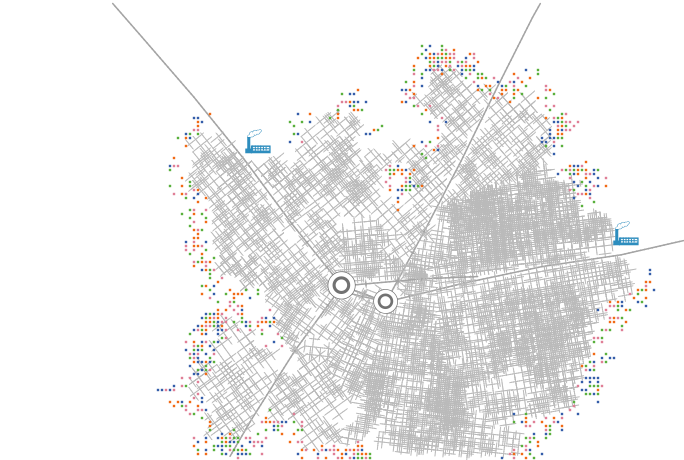
\includegraphics[width=0.33\textwidth]{Figures/PartI/Methodology/Reproducibility/stdView}
\hfill
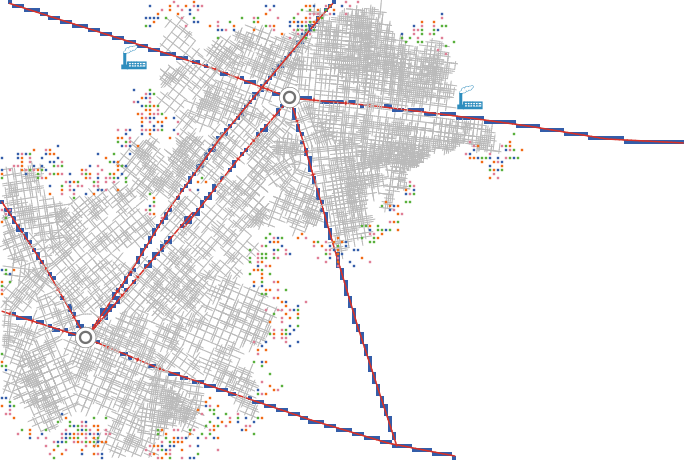
\includegraphics[width=0.33\textwidth]{Figures/PartI/Methodology/Reproducibility/ViewRoads}
\hfill
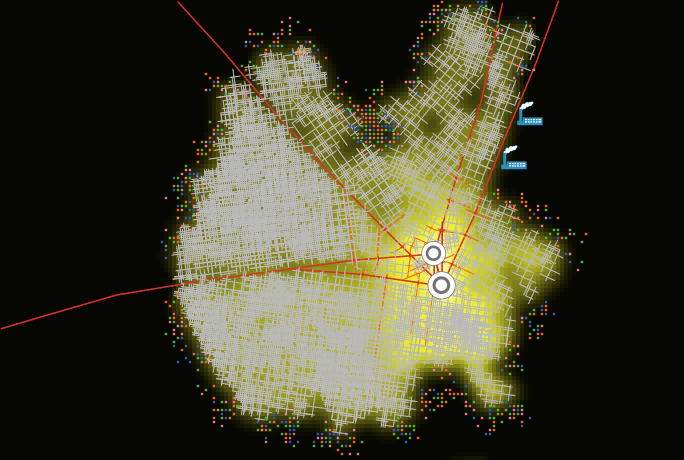
\includegraphics[width=0.33\textwidth]{Figures/PartI/Methodology/Reproducibility/landValues_cityFinished}
\caption[Reproducibility and visualization][Reproductibilité et visualisation]{Example of simple improvement in visualization that can help understanding mechanisms implied in the model. \textit{Left : } example of original output ; \textit{Middle : } visualization of main roads (in red) and underlying patches attribution, suggesting possible implementation bias in the use of discretized trace of roads to track their positions ; \textit{Right : }Visualization of land values using a more readable color gradient. This step confirms the hypothesis, through the form of value distribution, that the morphogenesis step is an unnecessary detour to generate a random field for which simple diffusion method should provide similar results, as detailed in the paragraph on implementation.}{}
\label{fig:example_tij_viz}
\end{figure}
%%%%%%%%%%%%%%%%%%%%%



\subsection{On the Need of Exactitude in Model Implementation}{Sue le besoin d'exactitude dans l'implémentation du modèle}

% Barthelemy paper, pb in model description/implementation
%  - test different analyses with possible biaises -

Possible divergences between model description in a paper and the effectively implemented processes may have grave consequences on the reproducibility of science. The road network growth model given in~\cite{barthelemy2008modeling} is one example that we are currently investigating. A strict implementation of model mechanisms provide slightly different results than the one presented in the paper, and as source code is not provided we need to test different hypotheses on possible mechanisms added by the programmer (that seems to be a connexion rule to intersections under a certain distance threshold). Lessons that could be possibly drawn from this examples are 
\begin{itemize}
\item the necessity of providing source code
\item the necessity of providing architecture description along with code (if model description is in a langage too far from architectural specifications) in order to identify possible implementation biaises
\item the necessity of performing and detailing explicitly model explorations, that would in that case have helped to identify the implementation bias.
\end{itemize}

The last point, if first not provided, may ensure a limited risk of scientific falsification as it may be more complicated to fake false exploration results than to effectively explore the model. A joint project currently done is the writing of a false modeling paper in the spirit of~\cite{zilsel2015canular}, in which opposite results to the effective results of a given model are provided, without providing model implementation. A first bunch of test is the acceptance of a clearly non-reproducible paper in diverse journals, possibly with a control on textual elements (using or not ``buzz-words'' associated to the journal, etc.). Depending on results, a second experiment may be tested with providing open source code for model implementation but still with false results, to verify if reviewers effectively try to reproduce results when they pretend to want the code (in reasonable computational power limits of course, HPC being not currently broadly available in Humanities).



\subsection{Perspectives}{Perspectives}


Again, reproducibility and transparency is a non-negotiable feature of contemporaneous science, along with Open practices and Open Access. Too much examples (see a very recent one in experimental economics~\cite{camerer2016evaluating}) show in various disciplines the lack of reproducibility of experiments, that is a falsification of previous results or a result in itself. Falsification is a costly practice, and even if necessary~\cite{chavalarias2005nobel}, could be made more efficient through more transparency and direct reproducibility, increase therein the global workflow of science. We develop in parallel of this thesis various tools aimed to ease reproducibility, for which an overview is given in appendix~\ref{app:workflow}.



%----------------------------------------------------------------------------------------

% Section : stochastic framework for urban growth


\newpage

\section{An unified framework for stochastic models of urban growth}{Un cadre unifié pour les modèles stichastiques de croissance urbaine}

Urban growth modeling fall in the case of tentatives to find self-consistent rules reproducing dynamics of an urban system, and thus in our logic of system morphogenesis. We examine here methodological issues linked to different frameworks of urban growth.

%%%%%%%%%%%%%%%%%%%%
\subsection{Introduction}{Introduction}
%%%%%%%%%%%%%%%%%%%%

Various stochastic models aiming to reproduce population patterns on large temporal and spatial scales (city systems) have been discussed across various fields of the literature, from economics to geography, including models proposed by physicists. We propose here a general framework that allows to include different famous models (in particular Gibrat, Simon and Preferential Attachment model) within an unified vision. It brings first an insight into epistemological debates on the relevance of models. Furthermore, bridges between models lead to the possible transfer of analytical results to some models that are not directly tractable.


Seminal models of urban growth are Simon~\cite{simon1955class} (later generalized as e.g. \cite{haran1973modified}) and Gibrat models. Many examples can be given across disciplines. \cite{benguigui2007dynamic} give an equation-based dynamical model, whereas \cite{gabaix1999zipf} solves a stationary model. \cite{Gabaix20042341} reviews urban growth approaches in economics. A model adapted from evolutive urban theory is solved in~\cite{favaro2011gibrat} and improves Gibrat models. The question of empirical scales at which it is consistent to study urban growth was also tackled in the particular case of France~\cite{bretagnolle2002time}. We stay to a certain level of tractability to include models as essence of our approach is links between models but do not make ontologic assumptions.




%%%%%%%%%%%%%%%%%%%%
\subsection{Framework}{Cadre de Travail}
%%%%%%%%%%%%%%%%%%%%


\paragraph{Presentation}
What we propose as a framework can be understood as a meta-model in the sense of~\cite{cottineau2015incremental}, i.e. an modular general modeling process within each model can be understood as a limit case or as a specific case of another model. More simply it should be a diagram of formal relations between models. The ontological aspect is also tackled by embedding the diagram into an ontological state space (which discretization corresponds to the ``bricks'' of the incremental construction of~\cite{cottineau2015incremental}). It constructs a sort of model classification or modelography.

We are still at the stage of different derivations of links between models that are presented hereafter.

%\subsubsection{Models Included}

%The following models are included in our framework. The list is arbitrary but aims to offer a broad view of disciplines concerned

%\subsubsection{Thematic Classification}


%\subsubsection{Framework Formulation}
%Diagram linking various models ; first embedded into time/population plane, cases Discrete/Continous. Other aspects more sparse (ex. spatialization) ; how represent it ?

%%%%%%%%%%%%%%%%%%%%
%\subsection{Models formulation}



%%%%%%%%%%%%%%%%%%%%
\subsection{Derivations}{Dérivations}

\subsubsection{Generalization of Preferential Attachment}{Généralisation de l'Attachement Préférentiel}

\cite{yamasaki2006preferential} give a generalization of the classical Preferential Attachment Network Growth model, as a birth and death model with evolving entities. More precisely, network units gain and lose population (equivalent to links connexions) at fixed probabilities, and new unit can be created at a fixed rate.

\subsubsection{Link between Gibrat and Preferential Attachment Models}{Lien entre Gibrat et Attachement Préférentiel}


\bpar{
Let consider a strictly positive growth Gibrat model given by $P_i(t)=R_i(t)\cdot P_{i}(t-1)$ with $R_i(t)>1$, $\mu_i(t)=\Eb{R_i(t)}$ and $\sigma_i(t)=\Eb{R_i(t)^2}$. On the other hand, we take a simple preferential attachment, with fixed attachment probability $\lambda \in [0,1]$ and new arrivants number $m>0$. We derive that Gibrat model can be statistically equivalent to a limit of the preferential attachment model, assuming that the moment-generating function of $R_i(t)$ exists. Classical distributions that could be used in that case, e.g. log-normal distribution, are entirely defined by two first moments, making this assumption reasonable.
}{
Considérons un modèle de croissance strictement positive de Gibrat donnée par $P_i(t)=R_i(t)\cdot P_{i}(t-1)$ avec $R_i(t)>1$, $\mu_i(t)=\Eb{R_i(t)}$ et $\sigma_i(t)=\Eb{R_i(t)^2}$. D'autre part, soit un modèle simple d'attachement préférentiel, avec une probabilité d'attachement $\lambda \in [0,1]$ et un nombre de nouveau arrivants $m>0$. Il est possible de dériver que le Gibrat est statistiquement équivalent à une limite de l'attachement préférentiel, sous l'hypothèse que toutes les fonctions génératrices des moments de $R_i(t)$ existent. Les distributions classiques qui peuvent être utilisées dans ce cas, e.g. une distribution normale ou log-normale, sont entièrement déterminées par leur deux premiers moments, ce qui rend cette hypothèse raisonnable.
}



\begin{lemma}
The limit of a Preferential Attachment model when $\lambda \ll 1$ is a linear-growth Gibrat model, with limit parameters $\mu_i(t)=1+\frac{\lambda}{m\cdot (t-1)}$.
\end{lemma}


\bpar{
The proof is given in Appendix~\ref{app:technical}.
}{
La preuve est donnée en Annexe~\ref{app:technical}.
}


\subsubsection{Link between Simon and Preferential Attachment}{Lien entre Simon et Attachement Préférentiel}
%\label{subsubsec:gibrat-simon}

A rewriting of Simon model yields a particular case of the generalized preferential attachment, in particular by vanishing death probability.

\subsubsection{Link between Favaro-Pumain and Gibrat}{Lien entre Favaro-Pumain et Gibrat}

\cite{favaro2011gibrat} generalizes Gibrat models with innovation propagation dynamics, being therefore a generalization of that model. Theoretically, a process-based model equivalent to the Favaro-pumain should then fill the missing case in model classification at the corresponding discretization. Simpop models do not fill that case as they stay at the scale of city systems, as for Marius models~\cite{cottineau2014evolution}. These must also have their counterparts in discrete microscopic formulation.

\subsubsection{Link between Bettencourt-West and Pumain}{Lien entre Bettencourt-West et Pumain}

We are considering to study Bettencourt-West model for urban scaling laws \cite{bettencourt2008large} as entering the stochastic urban growth framework as stationary component of a random growth model, but investigation are still ongoing.


\subsubsection{Other Models}{Autres modèles}

\cite{gabaix1999zipf} develops an economic model giving a Simon equivalent formulation. They in particular find out that in upper tail, proportional growth process occurs. We find the same result as a consequence of the derivation of the link between Gibrat and Preferential attachment models.




%%%%%%%%%%%%%%%%%%%%
%\subsection{Application and Perspectives}
%%%%%%%%%%%%%%%%%%%%







%%%%%%%%%%%%%%%%%%%%
%\subsection{Discussion}
%%%%%%%%%%%%%%%%%%%%

%%%%%%%%%%%%%%%%%%%%
%\subsection*{Conclusion}
%%%%%%%%%%%%%%%%%%%%





%----------------------------------------------------------------------------------------

\newpage


%  section : scaling sensitivity : useful ?


\section{Sensitivity of Urban Scaling Laws to Spatial Extent}{Sensibilité des Lois d'Echelle Urbaines à l'Etendue Spatiale}


\bpar{
At the center of evolutive urban theory are hierarchy and associated scaling laws. We develop here a brief methodological investigation on the sensitivity of scaling laws to city definition.
}{
Au centre de la théorie évolutive des villes se trouvent la hiérarchie et les lois d'échelle associées. Nous proposons ici un bref développement méthodologique sur la sensibilité des lois d'échelle à la définition de la ville.
}


%%%%%%%%%%%%%%%%%%%%
%\subsection{Introduction}



\bpar{
Scaling laws have been shown to be universal of urban systems at many scales and for many indicators. Recent studies question however the consistence of scaling exponents determination, as their value can vary significantly depending on thresholds used to define urban entities on which quantities are integrated, even crossing the qualitative border of linear scaling, from infra-linear to supra-linear scaling. We use a simple theoretical model of spatial distribution of densities and urban functions to show analytically that such behavior can be derived as a consequence of the type of spatial distribution and the method used. Numerical simulation confirm the theoretical results and reveals that results are reasonably independent of spatial kernel used to distribute density.
}{
Les lois d'échelle ont été montrées universelles des systèmes urbains à de nombreuses échelles et pour différents indicateurs. Des études récentes questionnent toutefois la cohérence de la détermination des exposants d'échelle, puisque leur valeur peut varier significativement selon les seuils utilisés pour définir les entités urbaines sur lesquelles les quantités urbaines sont intégrées, franchissant même dans certains cas la barrière qualitative de l'échelle linéaire, d'une loi infra-linéaire à une loi super-linéaire. Nous utilisons un modèle théorique simple de distribution spatiale des densités et des fonctions urbaines pour montrer analytiquement qu'un tel comportement peut être dérivé comme conséquence du type de distribution spatiale et de la méthode utilisée. Les simulations numériques confirment les résultats théoriques et révèle que les résultats sont raisonnablement indépendants du noyau spatial utilisé pour distribuer la densité.
}


\bpar{
Scaling laws for urban systems, starting from the well-known rank-size Zipf's law for city size distribution~\cite{gabaix1999zipf}, have been shown to be a recurrent feature of urban systems, at many scales and for many types of indicators. They reside in the empirical constatation that indicators computed on elements of an urban system, that can be cities for system of cities, but also smaller entities at a smaller scale, do fit relatively well a power-law distribution as a function of entity size, i.e. that for entity $i$ with population $P_i$, we have for an integrated quantity $A_i$, the relation $A_i \simeq A_0\cdot \left(\frac{P_i}{P_0}\right)^{\alpha}$. Scaling exponent $\alpha$ can be smaller or greater than 1, leading to infra or supralinear effects. Various thematic interpretation of this phenomena have been proposed, typically under the form of processes analysis. The economic literature has produced abundant work on the subject (see~\cite{Gabaix20042341} for a review), but that are generally weakly spatial, thus of poor interest to our approach that deals precisely with spatial organization. Simple economic rules such as energetic equilibria can lead to simple power-laws~\cite{bettencourt2008large} but are difficult to fit empirically. A interesting proposition by \noun{Pumain} is that they are intrinsically due to the evolutionary character of city systems, where complex emergent interaction between cities generate such global distributions~\cite{pumain2006evolutionary}. Although a tempting parallel can be done with self-organizing biological systems, \noun{Pumain} insists on the fact that the ergodicity assumption for such systems is not reasonable in the case of geographical systems and that the analogy can difficultly be exploited~\cite{pumain2012urban}. Other explanations have been proposed at other scales, such as the urban growth model at the mesoscopic scale (city scale) given in~\cite{2014arXiv1401.8200L} % TODO is this quote also relevant here ?
 that shows that the congestion within transportation networks may be one reason for city shapes and corresponding scaling laws. Note that ``classic'' urban growth models such as Gibrat's model do provide first order approximation of scaling systems, but that interactions between agents have to be incorporated into the model to obtain better fit on real data, such as the Favaro-Pumain model for innovation cycles propagation proposed in~\cite{favaro2011gibrat}, that generalize a Gibrat model for French cities with an ontology similar to Simpop models.
}{
Les lois d'échelle pour les systèmes urbains, en commençant par la bien connue loi rang-taille de Zipf pour la distribution des tailles des villes~\cite{gabaix1999zipf}, ont été montrées être une caractéristique récurrente des systèmes urbains, à différentes échelles et pour différents types d'indicateurs. Elles reposent sur la constatation empirique que des indicateurs calculés sur des éléments du système urbain, qui peuvent être les villes dans le cas d'un système de villes, mais aussi des entités plus petites à une plus petite échelle, suivent relativement bien une distribution en loi de puissance en fonction de la taille de l'entité, i.e. pour l'entité $i$ avec population $P_i$, on a pour une quantité intégrée $A_i$, la relation $A_i \simeq A_0\cdot \left(\frac{P_i}{P_0}\right)^{\alpha}$. Les exposants d'échelle $\alpha$ peuvent être plus petits ou plus grands que 1, menant à des effets infra ou supra-linéaires. Diverses interprétations thématiques de ce phénomène ont été proposées, typiquement sous la forme d'analyse des processus. La littérature économique contient une production abondante sur le sujet (voir~\cite{Gabaix20042341} pour une revue), mais est généralement faiblement spatiale, donc de faible intérêt pour notre approche qui s'intéresse particulièrement à l'organisation spatiale. Des règles économiques simples comme un équilibre énergétique peut conduire à de simples lois d'échelles~\cite{bettencourt2008large} mais sont difficiles à ajuster empiriquement. Une proposition intéressante par \noun{Pumain} est qu'elles sont intrinsèquement dues au caractère évolutionnaire des systèmes de villes, où l'émergence complexe par les interactions entre villes génère de telles distributions globales~\cite{pumain2006evolutionary}. Même si un parallèle tentant peut être fait avec les système biologiques auto-organisés % TODO here make a link with morphogenesis - depending if introduced before or not
 , \noun{Pumain} insiste sur le fait que l'hypothèse d'ergodicité pour de tels systèmes n'est pas raisonnable dans le cas de système géographiques et que l'analogie est difficilement exploitable~\cite{pumain2012urban}. D'autres explications ont été proposées à d'autres échelles, comme le modèle de croissance urbaine à échelle mesoscopique (échelle de la ville) donné dans~\cite{2014arXiv1401.8200L} qui montre que la congestion dans les réseaux de transport pourrait être une raison de la forme des villes et des lois d'échelle correspondantes. On peut noter que les modèles ``classiques'' de croissance urbaine comme le modèle de Gibrat~\cite{favaro2011gibrat} fournissent une approximation au premier ordre des systèmes % scaling systems = systèmes scalant ? ~ systèmes exhibant des lois d'échelle <- too long..
  exhibant des lois d'échelles, mais que les interactions entre agents doivent être incorporées dans le modèle pour obtenir un résultat plus fidèle aux données réelles, comme le modèle de Favaro-Pumain pour la propagation des cycles d'innovation proposé dans~\cite{favaro2011gibrat}, qui généralise un modèle de Gibrat pour la croissance des villes françaises avec une ontologie similaire à celle des modèles Simpop.
}


% TODO IDEE - take the FavaroPumain again, try to fit/compare with the IntGib-network model ? -- sort of benchmark, should be easy to implement


\bpar{
However, the blind application of scaling exponents computations was recently pointed as misleading in most cases~\cite{louf2014scaling} % TODO do not cite this empty "paper"
, confirmed by empirical works such as~\cite{2013arXiv1301.1674A} that showed the variability of computed exponents to the parameters defining urban areas, such as density thresholds. An ongoing work by Cottineau \& \textit{al.} presented at~\cite{cottineau2015scaling}, studies empirically for French Cities the influence of 3 parameters playing a role in city definition, that are a density threshold $\theta$ to delimitate boundaries of an urban area, a number of commuters threshold $\theta_c$ that is the proportion of commuters going to core area over which the unity is considered belonging to the area, and a cut-off parameter $P_c$ under which entities are not taken into account for the linear regression providing the scaling exponent. Remarquable results are that exponents can significantly vary and move from infra-linear to supra-linear when threshold varies. A systematic exploration of parameter space produces phase diagrams of exponents for various quantities. One question raising immediately is how these variation can be explained by the features of spatial distribution of variables. Do they result from intrinsic mechanisms present in the system or can they be explained more simply by the fact that the system is particularly spatialized ? We prove on a toy analytical model that even simple distributions can lead to such significant variations in the exponents, along one dimension of parameters (density threshold), directing the response towards the second explanation.
}{

}





%The rest of the section is organized as follows : we formalize the simple framework used and derive an analytical relation between estimated exponent and density threshold parameter. We then present a numerical implementation of the model that confirms numerically theoretical results, explore other form of kernels that would be less tractable, and study the sensitivity along two parameters. We finally discuss the implications of our results and further work needed.

The derivations in the simple case of exponential mixture density, are done in Appendix~\ref{app:technical}.

% TODO : mention way of fitting ; golden standard to fit power laws ? check thèse d'Olivier pour voir si le cutoff est appliqué ?







%----------------------------------------------------------------------------------------


\newpage


%  section : synthetic data control - introduces rochebrune paper, feasible correlation space etc, and forthcoming applications ?


\section{Statistical Control on Initial Conditions by Synthetic Data Generation}{Contrôle statistique pour les conditions initiales par génération de données synthétiques}

\subsection{Context}{Contexte}

When evaluating data-driven models, or even more simple partially data-driven models involving simplified parametrization, an unavoidable issue is the lack of control on ``underlying system parameters'' (what is a ill-defined notion but should be seen in our sense as parameters governing system dynamics). Indeed, a statistics extracted from running the model on enough different datasets can become strongly biased by the presence of confounding in the underlying real data, as it is impossible to know if result is due to processes the model tries to translate or to a hidden structure common to all data.

%Let illustrate the issue with a simple example.

We formalize briefly a proposition of method that would allow to add controls on meta-parameters, in the sense of parameters driving the represented system at a higher temporal and spatial scale, for a model of simulation. We make the hypothesis that such method is valid under constraints of disjonction for scales and/or ontologies between the model of simulation and the domain of meta-parameters.


\subsection{Description}{Description}

An advanced knowledge of the behavior of computational models on their parameter space is a necessary condition for deductions of thematic conclusions or their practical application~\cite{banos2013pour}. But the choice of varying parameters is always subjective, as some may be fixed by a real-world parametrization, or other may be interpreted as arbitrarily fixed initial conditions. It raises methodological and epistemological issues for the sensitivity analysis, as the scope of the model may become ill-defined.

Let consider the concrete example of the Schelling Segregation model~\cite{schelling1971dynamic}. One of its crucial features on which the literature has been rather controversial is the influence of the spatial structure of the container on which agents evolve.%~(\textit{Biblio Marion}). 
 The thematic aim of the project developed in~\cite{cottineau2015revisiting} is to clarify this point through a systematic model exploration. A methodological contribution is the construction of a framework allowing the analysis of the sensitivity of models to \emph{meta-parameters}, i.e. to parameters considered as fixed initial conditions (e.g. the spatial structure for the Schelling model), or to parameters of another model generating an initial configuration%, as detailed in Fig.~\ref{} \textit{[insert scheme describing the approach]}, 
 yielding thus a \emph{simple coupling} between models (serial coupling). The benefits of such an approach are various but include for example the knowledge of model behavior in an extended frame, the possibility of statistical control when regressing model outputs, a finer exploration of model derivatives than with a naive approach. Some remarks can be made on the approach :
\begin{itemize}
\item What knowledge are brought by adding the upstream model, rather than for example in the Schelling case exploring a large set of initial geometries ? 

$\rightarrow$ \textit{to obtain a sufficiently large set of initial configuration, one quickly needs a model to generate them ; in that case a quasi-random generation followed by a filtering on morphological constraint will be a morphogenesis model, which parameters are the ones of the generation and the filtering methods. Furthermore, as detailed further, the determination of the derivative of the downstream model is made possible by the coupling and knowledge of the upstream model.}
\item Statistical noise is added by coupling models

$\rightarrow$ \textit{Repetitions needed for convergence are indeed larger as the final expectance has to be determined by repeating on the first times the second model ; but it is exactly the same as exploring directly many configuration, to obtain statistical robustness in that case one must repeat on similar configurations.}

\item Complexity is added by coupling models

% check Varenne citation
$\rightarrow$ \textit{In the sense of Varenne~\cite{varenne2010framework} , coupling is simple and no complexity is thus added.}
\end{itemize}
 
%\paragraph{Context}

%Let $M_{m}$ a stochastic model of simulation, which inputs are to simplify initial conditions $D_0$ and parameters $\vec{\alpha}$, and output $M_{m}\left[\vec{\alpha},D_0\right](t)$ at a given time $t$. We assume that it is partially data-driven in the sense that $D_0$ is supposed to represent a real situation at a given time, and model performance is measured by the distance of its output at final time to the real situation at the corresponding time, i.e. error function is of the form $\norm{\Eb{\vec{g}(M_{m}\left[\vec{\alpha},D_0\right](t_f))}-\vec{g}(D_f)}$ where $\vec{g}$ is a deterministic field corresponding to given indicators.

%\paragraph{Position of the Problem}

%Evaluating the model on real data is rapidly limited in control possibilities, being restricted to the search of datasets allowing natural control groups. Furthermore, statistical behaviors are generally poorly characterized because of the small number of realizations. Working with synthetic data first allows to solve this issue of robustness of statistics, and then gives possibilities of control on some ``meta-parameters'' in the sense described before.




%%%%%%%%%%%%%%%%%%%%
\subsection{Formal Description}{Description Formelle}

%\subsubsection{Deterministic Formulation}

One has the composition of the derivative along the meta-parameter

\[
\partial_{\alpha}\left[M_u \circ M_d\right] = \left(\partial_{\alpha} M_u \circ M_d \right)\cdot \partial_{\alpha} M_d
\]

$\rightarrow$ \textit{the sensitivity of the downstream model (Schelling) can be determined by studying the serial coupling and the upstream model ; thematic knowledge : sensitivity to an implicit meta-parameter ; and computational gain : generation of controlled differentiates in the ``initial space'' is quasi impossible.}

%\subsubsection{Stochasticity}

The question of stochasticity in simply coupled models causes no additional issue as $\Eb{X}=\Eb{\Eb{X|Y}}$. It naturally multiplies the number of repetition needed for convergence what is the expected behavior.






%----------------------------------------------------------------------------------------

\newpage




\section[Spatio-temporal Correlations]{Linking dynamic and static spatio-temporal correlations under simplified assumptions}{Lien entre correlation spatio-temporelles statiques et dynamiques sous hypothèses simplifiées}

\label{sec:spatiotempcorrs}

Space and Time are both crucial for the study of geographical systems when aiming to understand \emph{processes} (by definition dynamical~\cite{hypergeo}) evolving in a \emph{spatial structure} in the sense of~\cite{dollfus1975some}. Space is more than coordinates for elements of the system, but a dimension in itself that drives interactions and thus system properties. Reading geographical systems from the point of view of \emph{spatio-temporal processes} emphasizes the fact that \emph{space actually matters}. Space and time are closely linked in such processes, and depending on the underlying mechanisms, one can expect to extract useful information from one on the other : in certain cases that we will investigate in this part, it is for example possible to learn about dynamics from static information. Spatio-temporal correlations approaches, linked to spatio-temporal dynamics, are present in very broad fields such as dynamical image processing (including video compression)~\cite{chalidabhongse1997fast,hansen2004accelerated,ke2007spatio}, target tracking~\cite{belouchrani1997direction,vuran2004spatio}, climate science~\cite{cressie1999classes}, Earth sciences~\cite{ma2002spatio}, city systems dynamics~\cite{hernando2015memory,pigozzi1980interurban}, among others.


\cite{cross1994spatiotemporal} : spatio-temporal chaos


The capture of neighborhood effects in statistical models is a wisely used practice in spatial statistics, as the technique of Geographically Weighted Regression illustrates~\cite{brunsdon1998geographically}. A possible interpretation among many definitions of spatial autocorrelation~\cite{griffith1992spatial} yields that by estimating a plausible characteristic distance for spatial correlations or auto-correlations, one can isolate independent effects between variables from effects due to neighborhood interactions\footnote{note that the formal link between models of spatial autocorrelation (see e.g. \cite{griffith2012advanced}) is not clear and should be further investigated}. The study of the spatial covariance structure is a cornerstone of advanced spatial statistics that was early formulated~\cite{griffith1980towards}. We propose now to study possible links between spatial and temporal correlations, using spatio-temporal covariance structure to infer information on dynamical processes.


\subsection{Notations}{Notations}

We consider a multivariate spatio-temporal stochastic process denoted by $\vec{Y}\left[\vec{x},t\right]$. At a given point $\vec{x}_0$ in space, we can define temporal covariance structure by
\[
\mathbf{C}_t (\vec{x}_0) = \Varb{\vec{Y}\left[\vec{x}_0, \cdot\right]}
\]

and spatial covariance structure at fixed time by
\[
\mathbf{C}_x (t) = \Varb{\vec{Y}\left[\cdot, t\right]}
\]

It is clear that these quantities will be in practice first ill-defined because of the difficulty in interpreting such a process by a spatio-temporal random variable, secondly highly non-stationary in space and time. We stay however at a theoretical level to gain structural knowledge, reviewing simple cases in which a formal link can be established.


\subsection{Wave Equation}{Equation des Ondes}

In the case of propagating waves, there is an immediate link. Let assume that a wave equation if verified by ``deterministic'' parts of components

\begin{equation}
c^2 \cdot \partial^2_{t} \bar{Y}_i = \Delta \bar{Y}_i
\end{equation}

with $Y_i = \bar{Y}_i + \varepsilon_i$. If errors are uncorrelated and processes are stationary, we have then directly

\begin{equation}
\mathbf{C}_t \left[ \partial^2_t Y_i , \partial^2_t Y_j \right] = \frac{1}{c^2} \cdot\mathbf{C}_x \left[ \Delta Y_i , \Delta Y_j \right]
\end{equation}

This gives us however few insight on real systems as local diffusion, stationary assumptions and uncorrelated noises are far from being verified in empirical situations.

\subsection{Fokker-Planck Equation}{Equation de Fokker-Planck}

An other interesting approach may when the process verifies a Fokker-Planck equation on probabilities of the state of the system when it is given by its position (diffusion of particles in that case)

\begin{equation}
\partial_t P(x_i,t) = - d \cdot \partial_x P(x_i,t) + \frac{\sigma^2}{2} \partial^2_x P(x_i,t)
\end{equation}

With no cross-correlation terms in the Fokker-Planck equation, covariance between processes vanish. We have finally in that case only a relation between averaged spatial and temporal variances that brings no information to our question.

\subsection{Master Equation}{Equation Maitresse}

In the case of a master equation on probabilities of discrete states of the system

\begin{equation}
\partial_t \vec{P} = \mathbb{W} \vec{P}
\end{equation}

we have then for state $i$, $\partial_t P_i = \sum_j W_{ij}P_j$. As this relation is at a fixed time we can average in time to obtain an equation on temporal covariance. It is not clear how to make the link with spatial covariance as these will depend on spatial specification of discrete states. This question is still under investigation.


\subsection{Consistent spatio-temporal sampling}{Echantillonnage spatial cohérent}

In a more empirical way, we propose to not assume any contraint of process dynamics but to however investigate how the computation of spatial correlations can inform on temporal correlations. We try to formulate easily verifiable assumptions under which this is possible.

We make the following assumptions on the spatio-temporal stochastic processes $Y_i\left[\vec{x},t\right]$ :
\begin{enumerate}
\item Local spatial autocorrelation is present and bounded by $l_{\rho}$ (in other words the processes are continuous in space) : at any $\vec{x}$ and $t$, $\left|\rho_{\norm{\Delta \vec{x}} < l_{\rho}}\left[Y_i (\vec{x}+\Delta \vec{x},t), Y_i (\vec{x},t) \right]\right| > 0$.
\item Processes are locally parametrized : $Y_i = Y_i\left[\alpha_i\right]$, where $\alpha_i (\vec{x})$ varies with $l_{\alpha}$, with $l_{\alpha} \gg l_{\rho}$.
\item Spatial correlations between processes have a sense at an intermediate scale $l$ such that $l_{\alpha}\gg l \gg l{\rho}$.
\item Processes covariance stationarity times scale as $\sqrt{l}$.
\item Local ergodicity is present at scale $l$ and dynamics are locally chaotic.
\end{enumerate}


Assumptions one to three can be tested empirically and allow to compare spatial correlation estimated on spatial samplings at scale $l$. Assumption four is more delicate as we are precisely constructing this methodology because we have no temporal information on processes. It is however typical of spatial diffusion processes, and population or innovation diffusion should verify this assumption. The last assumption can be tested if feasible space is known, by checking cribbing on image space on the spatial sample. Under these conditions, local spatial sampling is equivalent to temporal sampling and spatial correlation estimators provide estimator of temporal correlations.









%----------------------------------------------------------------------------------------

\newpage



\section[Generation of Correlated Synthetic Data]{Generation of Correlated Synthetic Data}{Génération de Données Synthétiques Corrélées}




\bpar{
Generation of hybrid synthetic data resembling real data to some criteria is an important methodological and thematic issue in most disciplines which study complex systems. Interdependencies between constituting elements, materialized within respective relations, lead to the emergence of macroscopic patterns. Being able to control the dependance structure and level within a synthetic dataset is thus a source of knowledge on system mechanisms. We propose a methodology consisting in the generation of synthetic datasets on which correlation structure is controlled. The method is applied in a first example on financial time-series and allows to understand the role of interferences between components at different scales on performances of a predictive model. A second application on a geographical system is then proposed, in which the weak coupling between a population density model and a network morphogenesis model allows to simulate territorial configurations. The calibration on morphological objective on european data and intensive model exploration unveils a large spectrum of feasible correlations between morphological and network measures. We demonstrate therein the flexibility of our method and the variety of possible applications.
}{
La génération de données synthétiques hybrides similaires à des données réelles présente des enjeux méthodologiques et thématiques pour la plupart des disciplines dont l'objet est l'étude de systèmes complexes. Comme l'interdépendance entre les éléments constitutifs d'un système, matérialisée par leur relations, conduit à l'émergence de ses propriétés macroscopiques, une possibilité de contrôle de l'intensité des dépendances dans un jeu de données synthétiques est un instrument de connaissance du comportement du système. Nous proposons une méthodologie de génération de données synthétiques hybrides sur lequel la structure de correlation est contrôlée. La méthode est illustrée sur des séries temporelles financières et permet l'étude de l'interférence entre composantes à différentes fréquences sur la performance d'un modèle prédictif, en fonction des correlations entre composantes à différentes échelles. On présente ensuite une application à un système géographique, dans laquelle le couplage faible d'un modèle de distribution de densité de population avec un modèle de génération de réseau permet la simulation de configurations territoriales, qui sont calibrées selon des objectifs morphologiques sur l'ensemble de l'Europe. L'exploration intensive du modèle permet l'obtention d'un large spectre de valeurs pour la matrice de correlation entre mesures morphologiques et mesures du réseau. On démontre ainsi les possibilités d'applications variées et les potentialités de la méthode.
}




\subsection{Context}{Contexte}

\bpar{

The use of synthetic data, in the sense of statistical populations generated randomly under constraints of patterns proximity to the studied system, is a widely used methodology, and more particularly in disciplines related to complex systems such as therapeutic evaluation~\cite{abadie2010synthetic}, territorial science~\cite{moeckel2003creating,pritchard2009advances}, machine learning~\cite{bolon2013review} or bio-informatics~\cite{van2006syntren}. It can consist in data desegregation by creation of a microscopic population with fixed macroscopic properties, or in the creation of new populations at the same scale than a given sample, with criteria of proximity to the real sample. These criteria will depend on expected applications and can for example vary from a restrictive statistical fit on given indicators, to weaker assumptions of similarity in aggregated patterns. In the case of chaotic systems, or systems where emergence plays a strong role, a microscopic property does not directly imply given macroscopic patterns, which reproduction is indeed one aim of modeling and simulation practices in complexity science. With the rise of new computational paradigms~\cite{arthur2015complexity}, data (simulated, measured or hybrid) shape our understanding of complex systems. Methodological tools for data-mining and modeling and simulation (including the generation of synthetic data) are therefore crucial to be developed.
}{
L'utilisation de données synthétiques, au sens de populations statistiques d'individus générées aléatoirement sous la contrainte de reproduire certaines caractéristiques du système étudié, est une pratique méthodologique largement répandue dans de nombreuses disciplines, et particulièrement pour des problématiques liées aux systèmes complexes, telles que par exemple l'évaluation thérapeutique~\cite{abadie2010synthetic}, l'étude des systèmes territoriaux~\cite{moeckel2003creating,pritchard2009advances}, l'apprentissage statistique~\cite{bolon2013review} ou la bio-informatique~\cite{van2006syntren}. Il peut s'agir d'une désagrégation par création d'une population au niveau microscopique présentant des caractéristiques macroscopiques données, ou bien de la création de nouvelles populations au même niveau d'agrégation qu'un échantillon donné avec un critère de ressemblance aux données réelles.  Le niveau de ce critère peut dépendra des applications attendues et peut par exemple aller de la fidélité des distributions statistiques pour un certain nombre d'indicateurs à des contraintes plus faibles de valeurs pour des indicateurs agrégés, c'est à dire l'existence de motifs macroscopiques similaires. Dans le cas de systèmes chaotiques ou présentant de fortes caractéristiques d'émergence, une contrainte microscopique n'implique pas nécessairement le respect des motifs macroscopiques, et arriver à les reproduire est justement un des enjeux des pratiques de modélisation et simulation en sciences de la complexité. La donnée, qu'elle soit simulée, mesurée ou hybride est au coeur de l'étude des systèmes complexes de par la maturation de nouvelles approches computationelles~\cite{arthur2015complexity}, il est donc essentiel d'étudier des procédures d'extraction d'information des données (fouille de données) et de simulation d'une information similaire (génération de données synthétiques).
}




\bpar{
Whereas first order (in the sense of distribution moments) is generally well used, it is not systematic nor simple to control generated data structure at second order, i.e. covariance structure between generated variables. Some specific examples can be found, such as in~\cite{ye2011investigation} where the sensitivity of discrete choices models to the distributions of inputs and to their dependance structure is examined. It is also possible to interpret complex networks generative models~\cite{newman2003structure} as the production of an interdependence structure for a system, contained within link topology. We introduce here a generic method taking into account dependance structure for the generation of synthetic datasets, more precisely with the mean of controlled correlation matrices.
}{
Si le premier ordre est de manière générale bien maîtrisé, il n'est pas systématique ni aisé de contrôler le second ordre, c'est à dire les structures de covariance entre les variables générées, même si des exemples spécifiques existent, comme dans~\cite{ye2011investigation} où la sensibilité des sorties de modèles de choix discrets à la forme des distributions des variables aléatoires ainsi qu'à leur structures de dépendance. Il est également possible d'interpréter les modèles de génération de réseaux complexes~\cite{newman2003structure} comme la création d'une structure d'interdépendance au sein d'un système, représentée par la topologie des liens. Nous proposons ici une méthode générique prenant en compte l'interdépendance lors de la génération de données synthétiques, sous la forme de correlations.
}



\bpar{
Domain-specific methods aforementioned are too broad to be summarized into a same formalism. We propose a framework as generic as possible, centered on the control of correlations structure in synthetic data.
}{
L'ensemble des méthodologies mentionnées en introduction sont trop variées pour être résumées par un même formalisme. Nous proposons ici une formulation générique ne dépendant pas du domaine d'application, ciblée sur le contrôle de la structure de correlation des données synthétiques.
}


%%%%%%%%%%%%%
\subsection{Formalization}{Formalisation}


\bpar{
Let $\vec{X}_I$ a multidimensional stochastic process (that can be indexed e.g. with time in the case of time-series, but also space, or discrete set abstract indexation). We assume given a real dataset $\mathbf{X}=(X_{i,j})$, interpreted as a set of realizations of the stochastic process. We propose to generate a statistical population $\mathbf{\tilde{X}}=\tilde{X}_{i,j}$ such that
\begin{enumerate}
\item a given criteria of proximity to data is verified, i.e. given a precision $\varepsilon$ and an indicator $f$, we have $\norm{f(\mathbf{X})-f(\mathbf{\tilde{X}})} < \varepsilon$
\item level of correlation is controlled, i.e. given a matrix $R$ fixing correlation structure (symmetric matrix with coefficients in $[-1,1]$ and unity diagonal), we have $\hat{\Var{}}\left[(\tilde{X}_i)\right] = \Sigma R \Sigma$, where the standard deviation diagonal matrix $\Sigma$ is estimated on the synthetic population.
\end{enumerate}
}{
Soit un processus stochastique multidimensionnel $\vec{X}_I$ (l'ensemble d'indexation pouvant être par exemple le temps dans le cas de séries temporelles, l'espace, ou une indexation quelconque). On se propose, à partir d'un jeu de réalisations $\mathbf{X}=(X_{i,j})$, de générer une population statistique $\mathbf{\tilde{X}}=\tilde{X}_{i,j}$ telle que
\begin{enumerate}
\item d'une part un certain critère de proximité aux données est vérifié, i.e. étant donné une précision $\varepsilon$ et un indicateur $f$, $\norm{f(\mathbf{X})-f(\mathbf{\tilde{X}})} < \varepsilon$
\item d'autre part le niveau de correlation est controlé, i.e. étant donné une matrice fixant une structure de covariance $R$, $\Varb{(\tilde{X}_i)} = R$, où la matrice de variance/covariance est estimée sur la population synthétique.
\end{enumerate}
}


\bpar{
The second requirement will generally be conditional to parameter values determining generation procedure, either generation models being simple or complex ($R$ itself is a parameter). Formally, synthetic processes are parametric families $\tilde{X}_i[\vec{\alpha}]$. % TODO : explicit the fact that real data may come out of different parameter values ?
We propose to apply the methodology on very different examples, both typical of complex systems : financial high-frequency time-series and territorial systems. We illustrate the flexibility of the method, and claim to help building interdisciplinary bridges by methodology transposition and reasoning analogy. In the first case, proximity to data is the equality of signals at a fundamental frequency, to which higher frequency synthetic components with controlled correlations are superposed. It follows a logic of hybrid data for which hypothesis or model testing is done on a more realistic context than on purely synthetic data. This example that has no thematic link with the thesis, is presented in Appendic~\ref{app:syntheticdata}. In the second case, morphological calibration of a population density distribution model allows to respect real data proximity. Correlations of urban form with transportation network measures are empirically obtained by exploration of coupling with a network morphogenesis model. The control is in this case indirect as feasible space is empirically determined.
}{
La satisfaction du deuxième point sera généralement conditionnée par la valeur de paramètres, dont dépendra la procédure de génération, qu'il s'agisse de modèles simples ou complexes. Formellement, les processus synthétiques sont des familles paramétriques $\tilde{X}_i[\vec{\alpha}]$. Nous proposons de décliner cette méthode sur deux exemples très différents mais tous deux typiques des systèmes complexes : des séries temporelles financières à haute fréquence, et les systèmes territoriaux. On illustre ainsi la flexibilité de la logique, ouvrant des portes interdisciplinaires par l'exportation de méthodes ou raisonnements par exemple. Dans le premier cas, la proximité aux données est l'égalité des signaux à une fréquence fondamentale, auxquels on superpose des composantes synthétiques dont il est facile de contrôler le niveau de correlation. On se place dans une logique de données hybrides, pour tester des hypothèses ou modèles dans un contexte plus proche de la réalité que sur des données purement synthétiques. Cet exemple, sans rapport thématique avec la thèse, est présenté en Appendice~\ref{app:syntheticdata}. Dans le deuxième cas, la calibration morphologique d'un modèle de distribution de densité de peuplement permet de respecter le critère de proximité aux données. Les correlations de la forme urbaine avec celle d'un réseau de transport sont ensuite obtenues empiriquement par exploration du couplage avec un modèle de génération de réseau. Leur contrôle est dans ce cas indirect puisque constaté empiriquement.
}

















%----------------------------------------------------------------------------------------

\newpage



\section[Big Data and Computation]{For a cautious use of big data and computation}{Pour un usage raisonné des données massives et de la computation}




\bpar{
The so-called \emph{big data revolution} resides as much in the availability of large datasets of novel and various types as in the always increasing available computational power. Although the \emph{computational shift} (\cite{arthur2015complexity}) is central for a science aware of complexity and is undeniably the basis of future modeling practices in geography as \cite{banos2013pour} points out, we argue that both \emph{data deluge} and \emph{computational potentialities} are dangerous if not framed into a proper theoretical and formal framework. The first may bias research directions towards available datasets (as e.g. numerous twitter mobility studies) with the risk to disconnect from a theoretical background, whereas the second may overshadow preliminaries analytical resolutions essential for a consistent use of simulations. We argue that the conditions for most of results in this thesis are indeed the ones endangered by incautious big-data enthusiasm, concluding that a main challenge for future Geocomputation is a wise integration of novel practices within the existing body of knowledge.
}{
La soi-disante \emph{révolution des données massives} réside autant dans la disponibilité de grands jeux de données de nouveaux types variés, que dans la puissance de calcul potentielle toujours en augmentation. Même si le \emph{tournant computationnel} (\cite{arthur2015complexity}) est central pour une science consciente de la complexité et est sans douter la base des pratiques de modélisation futures en géographie comme \cite{banos2013pour} souligne, nous soutenons que à la fois le \emph{déluge de données} et les \emph{capacités de calcul} sont dangereuses si non cadrées dans un cadre théorique et formel propre. Le premier peut biaiser les directions de recherche vers les jeux de données disponibles (comme par exemple les nombreuses étude de mobilité se basant sur twitter) avec le risque de se déconnecter d'un fond théorique, tandis que le second peut occulter des résolutions analytiques préliminaires essentielles pour un usage cohérent des simulations. Nous avançons que les conditions pour la majorité des résultats dans cette thèse sont en effet ceux mis en danger par un enthousiasme inconsidéré pour les données massives, tirant la conclusion qu'un challenge majeur pour la géocomputation future est une intégration sage des nouvelles pratiques au sein du corpus existant de connaissances.
}


\bpar{
The computational power available seems to follow an exponential trend, as some kind of Moore's law. Both effective Moore's law for hardware, and improvement of softwares and algorithms, combined with a democratization of access to large scale simulation facilities, makes always more and more CPU time available for the social scientist (and to the scientist in general but this shift happened quite before in other fields, as e.g. CERN is leading in cloud computing and grid computation). About 10 years ago, \cite{gleyze2005vulnerabilite} concluded that network analysis, for the case of Parisian public transportation network, was ``limited by computation''. Today most of these analyses would be quickly done on a personal computer with appropriated software and coding: \cite{2015arXiv151201268L} is a witness of such a progress, introducing new indicators with a higher computational complexity, computed on larger networks. The same parallel can be done for the Simpop models: the first Simpop models at the beginning of the millenium~\cite{sanders1997simpop} were ``calibrated'' by hand, whereas \cite{cottineau2015modular} calibrates the multi-modeling Marius model and~\cite{schmitt2014half} calibrates very precisely the SimpopLocal model, both on grid with billions of simulations. A last example, the field of Space Syntax, witnessed a long path and tremendous progresses from its theoretical origins~\cite{hillier1989social} to recent large-scale applications~\cite{hillier2016fourth}.
}{
La puissance de calcul disponible semble suivre un tendance exponentielle, comme une sorte de loi de Moore. Grace à d'une part la loi de Moore effective pour le matériel, d'autre part l'amélioration des logiciels et algorithmes, conjointement avec une démocratisation de l'accès au infrastructures de simulation à grande échelle, permet à toujours plus de temps processeur d'être disponible pour le chercheur en sciences sociales (et pour le scientifique en général, mais cette mutation a déjà été opérée depuis plus longtemps dans d'autres domaines, puisque par exemple le CERN est à la pointe en terme de calcul distant et sur grille). Il y a environ une dizaine d'année, \cite{gleyze2005vulnerabilite} était forcé de conclure que les analyses de réseau, pour les transports publics parisiens, étaient ``limitées par le calcul''. Aujourd'hui la plupart des mêmes analyses seraient rapidement réglée sur un ordinateur personnel avec les logiciels et programmes appropriés : \cite{2015arXiv151201268L} est un témoin d'un tel progrès, introduisant des nouveaux indicateurs avec une plus grande complexité de calcul, qui sont calculés sur des réseaux à grande échelle. Le même parallèle peut être fait pour les modèles Simpop : les premiers modèles Simpop au début du millénaire~\cite{sanders1997simpop} étaient ``calibrés'' à la main, tandis que \cite{cottineau2015modular} calibre le modèle Marius en multi-modélisation et~\cite{schmitt2014half} calibre très précisément le modèle SimpopLocal, chacun sur la grille avec des milliards de simulations. Un dernier exemple, le champ de la \emph{Space Syntax}, a témoigné d'une longue route et de progrès considérables depuis ses origines théoriques~\cite{hillier1989social} jusqu'à ses récentes applications à grande échelle~\cite{hillier2016fourth}.
}



\bpar{
Concerning the new and ``big'' data available, it is clear that always larger dataset are available and always newer type of data are available. Numerous examples of fields of application can be given. For example, mobility can now be studied from various entries, such as new data from smart transportation systems~\cite{o2014mining}, from social networks~\cite{frank2014constructing}, or other more exotic data such as mobile phone data~\cite{de2016death}. In an other spirit, the opening of ``classic'' datasets (such as city dashboards, open data government initiatives) should allow ever more meta-analyses. New ways to do research and produce data are also raising, towards more interactive and crowd-sourced initiatives. For example, \cite{2016arXiv160606162C} describes a web-application aimed at presenting a meta-analysis of Zipf's law across numerous datasets, but in particular features an upload option, where the user can upload its own dataset and add it to the meta-analysis. Other applications allow interactive exploration of scientific literature for a better knowledge of a complex scientific landscape, as~\cite{cybergeo20} does.
}{
Concernant les nouvelles données ``massives'' qui sont disponibles, il est clair que des quantités toujours plus grandes et des types toujours nouveaux sont disponibles. De nombreux exemples de champs d'application peuvent être donnés. La mobilité en est typique, puisque étudiée selon divers points de vue, comme les nouvelles données issues des systèmes de transport intelligents~\cite{o2014mining}, des réseaux sociaux~\cite{frank2014constructing}, ou des données plus exotiques comme des données de téléphonie mobile~\cite{de2016death}. Dans un autre esprit, l'ouverture de jeux de données ``classiques'' (comme les applications synthétiques urbaines, les initiatives gouvernementales pour les données ouvertes) devrait pouvoir toujours plus de méta-analyses. De nouvelles façon de pratiquer la recherche et produire des données sont également en train d'émerger, vers des initiatives plus interactives et venant de l'utilisateur. Ainsi, \cite{2016arXiv160606162C} décrit une application web ayant pour but de présenter une méta-analyse de la loi de Zipf sur de nombreux jeux de données, mais en particulier inclut une option de dépôt, à travers laquelle l'utilisateur peut télécharger sont propre jeu de données et l'inclure dans la méta-analyse. D'autres applications permettent l'exploration interactive de la littérature scientifique pour une meilleure connaissance d'un horizon scientifique complexe, comme~\cite{cybergeo20} fait.
}


\bpar{
As always the picture is naturally not as bright as it seems to be at first sight, and the green grass that we try to go eating in the neighbor's field quickly turns into a sad reality. Indeed, the purpose and motivation are fuzzy and one can get lost. Some examples speaks for themselves. \cite{barthelemy2013self} introduces a new dataset and rather new methods to quantify road network evolution, but the results, on which the authors seem to be astonished, are that a transition occurred in Paris at the Haussmann period. Any historian of urbanism would be puzzled by the exact purpose of the paper, as in the end a vague and bizarre feeling of reinventing the wheel floats in the air. The use of computation can also be exaggerated, and in the case of agent-based modeling it can be illustrated by the example of~\cite{axtell2016120}, for which the aim at simulating the system at scale 1:1 seems to be far from initial motivations and justifications for agent-based modeling, and may even give arguments to mainstream economists that denigrate easily ABMS. Other anecdotes raise worries: \cite{robin_cura_2014_11415} is a web application that wastes computational ressources to simulate Gaussian distributions for a Gibrat model in order to compute their mean and variance, that are input parameters of the model. It basically checks the Central Limit Theorem, which is a priori well accepted among most scientists. Otherwise, the full distribution given by a Gibrat model is theoretically known as it was fully solved e.g. by \cite{gabaix1999zipf}. Recently on the French speaking diffusion list \emph{Geotamtam}, a sudden rush around \emph{Pokemon Go} data seemed to answer more to an urgent unexplained need to exploit this new data source before anyone else rather than an elaborated theoretical construction. Simple existing accurate datasets, such as historical cities population (for France the Pumain-INED database for example), are far from being fully exploited and it may be more important to focus on these already existing classic data. One must also be aware of the possible misleading applications of some results: \cite{louail2016crowdsourcing} makes a very good analysis of potential redistribution of bank card transactions within a city, but pushes the results as possible basis for social equity policy recommandation by acting on mobility, forgetting that urban form and function are coupled in a complex way and that moving transactions from one place to the other involves far more complex processes than policies (even in a country like China were policies are actually enforced with a hand of steel).
}{
Comme toujours la situation n'est naturellement pas aussi idyllique qu'elle semble être au premier abord, et l'herbe verte du pré du voisin que nous pouvons être tentés d'aller brouter se transforme rapidement en un triste fumier. En effet, les objectifs et motivations sont flous et on peut facilement s'y perdre. Des illustrations parleront d'elles-même. \cite{barthelemy2013self} introduit un nouveau jeu de données et des méthodes relativement nouvelles pour quantifier l'évolution du réseau de rues, mais les résultats, sur lesquels les auteurs semblent s'étonner, sont qu'une transition a eu lieu à Paris à l'époque d'Haussmann. Tout historien de l'urbanisme s'interrogerait sur le but exact de l'étude, puisque à la fin un sentiment étrange de réinvention de la roue flotte dans l'air. L'utilisation des ressources de calcul peut également être exagéré, et dans le cas de la modélisation multi-agent, on peut citer~\cite{axtell2016120}, pour lequel l'objectif de simuler le système à l'échelle 1:1 semble être loin des motivations et justifications originelles de la modélisation agent, et pourrait même donner des arguments aux économistes \emph{mainstream} qui dénigrent facilement les ABMS. D'autres anecdotes peuvent inquiéter : \cite{robin_cura_2014_11415} est une application web qui gâche des ressources de calcul  pour simuler des distributions Gaussiennes afin de calculer pour un modèle de Gibrat, afin de calculer leur moyenne et variance, qui sont des paramètres d'entrée du modèle. En résumé, cela revient à vérifier le Théorème de la Limite Centrale, qui est a priori assez accepté par la plupart des scientifiques. D'autre part, la distribution complète donnée par un modèle de Gibrat est entièrement connue théoriquement comme résolu e.g. par~\cite{gabaix1999zipf}. Récemment, sur la liste de diffusion de géographie francophone \emph{Geotamtam}, un soudain engouement autour des données issues de \emph{Pokemon Go} a semblé répondre plus à un besoin urgent et inexpliqué d'exploiter cette source de données avant tous les autres, plutôt qu'à des considérations théoriques élaborées. Des jeux de données existant et précis, comme la population historiques des villes (pour la France la base Pumain-INED par exemple), sont loin d'être entièrement exploités et il pourrait être plus pertinent de se concentrer sur ces jeux de données classiques qui existent déjà. De même, il faut être conscient des possibles applications de résultats basée sur des malentendus : \cite{louail2016crowdsourcing} fait une très bonne analyse de la redistribution potentielle des transactions de carte bancaire au sein d'une ville, mais présente les résultats comme la base possible de recommandations de politiques pour une équité sociale en agissant sur la mobilité, oubliant que la forme et les fonctions urbaines sont couplés de manière complexe et que déplacer des transactions d'un endroit à un autre implique des processus bien plus complexes que des régulations directes (même dans un pays comme la Chine ou les régulations sont effectivement mise en place et imposées d'une main de fer).
}




\bpar{
Our main claim here is that the computational shift and simulation practices will be central in geography, but may also be dangerous, for the reasons illustrated above, i.e. that data deluge may impose research subjects and elude theory, and that computation may elude model construction and solving. A stronger link is required between computational practices, computer science, mathematics, statistics and theoretical geography. Theoretical and Quantitative Geography is at the center of this dynamic, as it was its initial purpose that seems forgotten in some cases. It implies the need for elaborated theories integrated with conscious simulation practices. In other words we can answer complementary naive questions that have however to be tackled one and for once. If a theory-free quantitative geography would be possible, the answer if naturally no as it is close to the trap of black-box data-mining analysis. Whatever is done in that case, the results will have a very poor explanatory power, as they can exhibit relations but not reconstruct processes. On an other hand, the possibility of a purely computational quantitative geography is a dangerous vision: even gaining three orders of magnitudes in computational power does not solve the dimensionality curse. In our work here, without theory, we would not know which objects, measures and properties to look at (e.g. multi-scale and dynamical nature of processes), and without analytics, it would be sometimes difficult to draw conclusions from empirical analysis. Nothing is really new here but this position has to be stated and stood up, precisely because our work will use this kind of tools, trying to advance on a thin and fragile edge, with the void of the unfunded theoretical charlatanism on one side and the abyss of the technocratic blind drowning in foolish amounts of data. More than ever we need simple but powerful and funded theories {\`a}-la-Occam~\cite{batty2016theoretical}, to allow a wise integration of new techniques into existing knowledge.
}{
Notre principal argument est que le tournant computationnel et les pratiques de simulation seront centrales en géographie, mais peuvent également être dangereux, pour les raisons illustrées ci-dessus, i.e. que le déluge de données peut imposer les sujets de recherche et occulter la théorie, et que la computation peut éluder la construction et la résolution de modèles. Un lien plus fort est nécessaire entre les pratiques de calcul, l'informatique, les mathématiques, les statistiques et la géographie théorique. La Géographie Théorique et Quantitative est au centre de cette dynamique, puisqu'il s'agit de sa motivation initiale principale qui semble oubliée dans certains cas. Cela implique un besoin de recherche de théorie élaborées intégrées avec des pratiques de simulation conscientes. En d'autres mots, on peut répondre à des questions naïves complémentaires qui ont toutefois besoin d'être traitées une bonne fois pour toutes. Si une géographie quantitative libérée de la théorie serait possible, la réponse est naturellement non 
}


 
% multi-modeling and model families (see Cottineau, Rey and Reuillon presentation) as one way to do that ?

% Interdisciplinarity (and Nexus ?!) necessary to achieve that.









%%%%%%%%%%%%%%%%%%%%%%%%%%%%%



%%%%%%%%%%%%%%%%%%%%%%%%%%%%%
% Robustness Discrepancy
% TODO : included in methodological part ?

\newpage

\section{A Discrepancy-based Framework to Compare Robustness between Multi-Attribute Evaluations}{Un Cadre basé sur la Discrépance pour Comparer la Robustesse des Evaluations Multi-attributs} 

\label{sec:robustness}


%----------------------------------------------------------------------------------------



\bpar{
Multi-objective evaluation is a necessary aspect when managing complex systems, as the intrinsic complexity of a system is generally closely linked to the potential number of optimization objectives. However, an evaluation makes no sense without its robustness being given (in the sense of its reliability). Statistical robustness computation methods are highly dependent of underlying statistical models. We propose a formulation of a model-independent framework in the case of integrated aggregated indicators (multi-attribute evaluation), that allows to define a relative measure of robustness taking into account data structure and indicator values. We implement and apply it to a synthetic case of urban systems based on Paris districts geography, and to real data for evaluation of income segregation for Greater Paris metropolitan area. First numerical results show the potentialities of this new method. Furthermore, its relative independence to system type and model may position it as an alternative to classical statistical robustness methods.
}{
Les évaluations multi-objectifs sont un aspect essentiel de la gestion de systèmes complexes, puisque la complexité intrinsèque d'un système est généralement étroitement liée au nombre d'objectifs d'optimisation potentiels. Cependant, une évaluation ne fait pas sens si sa robustesse, au sens de sa fiabilité, n'est pas donnée. Les méthodes statistiques usuelles fournissant une mesure de robustesse sont très dépendantes des modèles sous-jacents. Nous proposons une formulation d'un cadre indépendant du modèle, dans le cas d'indicateurs intégrés et agrégés (évaluation multi-attributs), qui permet de définir une mesure de robustesse relative prenant en compte la structure des données et les valeurs des indicateurs. La méthode est testée sur données urbaines synthétiques associées aux arrondissements de Paris, et à des données réelles de revenus pour l'évaluation de la ségrégation urbaine dans la région métropolitaine du Grand Paris. Les premiers résultats numériques montrent les potentialités de cette nouvelle méthode. De plus, sa relative indépendance au type de système et au modèle pourrait la positionner comme une alternative aux méthodes statistiques classiques d'évaluation de la robustesse.
}


%%%%%%%%%%%%%%%%
%% Intro
%%%%%%%%%%%%%%%%
\subsection{Introduction}{Introduction}

%%%%%%%%%%%%%%%%
\subsubsection{General Context}{Contexte Général}


\bpar{
Multi-objective problems are organically linked to the complexity of underlying systems. Indeed, either in the field of \emph{Complex Industrial Systems}, in the sense of engineered systems, where construction of Systems of Systems (SoS) by coupling and integration often leads to contradictory objectives~\cite{marler2004survey}, or in the field of \emph{Natural Complex Systems}, in the sense of non engineered physical, biological or social systems that exhibit emergence and self-organization properties, where objectives can e.g. be the result of heterogeneous interacting agents (see~\cite{newman2011complex} for a large survey of systems concerned by this approach), multi-objective optimization can be explicitly introduced to study or design the system but is often already implicitly ruling the internal mechanisms of the system. The case of socio-technical Complex Systems is particularly interesting as, following~\cite{haken2003face}, they can be seen as hybrid systems embedding social agents into ``technical artifacts'' (sometimes to an unexpected degree creating what \noun{Picon} describes as \emph{cyborgs}~\cite{picon2013smart}), and thus cumulate propensity to be at the origin of multi-objective issues\footnote{We design by \emph{Multi-Objective Evaluation} all practices including the computation of multiple indicators of a system (it can be multi-objective optimization for system design, multi-objective evaluation of an existing system, multi-attribute evaluation ; our particular framework corresponds to the last case).}. The new notion of \emph{eco-districts}~\cite{souami2012ecoquartiers} is a typical example where sustainability implies contradictory objectives. The example of transportation systems, which conception shifted during the second half of the 20th century from cost-benefit analysis to multi-criteria decision-making, is also typical of such systems~\cite{bavoux2005geographie}. Geographical system are now well studied from such a point of view in particular thanks to the integration of multi-objective frameworks within Geographical Information Systems~\cite{carver1991integrating}. As for the micro-case of eco-districts, meso and macro urban planning and design may be made sustainable through indicators evaluation~\cite{jegou2012evaluation}.
}{
Les problèmes multi-objectifs sont organiquement liés à la complexité des systèmes sous-jacents. En effet, que ce soit dans le champ des \emph{Systèmes Complexes Industriels}, dans le sens de systèmes conçus par ingénierie, où la construction de Systèmes de Systèmes (SoS) par couplage et intégration induit souvent des objectifs contradictoires~\cite{marler2004survey}, ou dans le champ des \emph{Systèmes Complexes Naturels}, au sens de systèmes non désignés, physiques, biologiques ou sociaux, qui présentent des propriétés d'émergence et d'auto-organisation, pour lesquels les objectifs peuvent e.g. être le résultat de l'interaction d'agents hétérogènes (voir~\cite{newman2011complex} pour une revue étendue des types de systèmes concernés par cette approche), l'optimisation multi-objectifs peut être explicitement introduite pour étudier ou désigner le système, mais régit généralement déjà implicitement les mécanismes internes du système. Le cas des Systèmes Complexes Sociaux-techniques est particulièrement intéressant puisque selon Haken~\cite{haken2003face}, ils peuvent être vus comme des systèmes hybrides embarquant des agents sociaux dans des ``artefacts techniques'' (parfois jusqu'à un niveau inattendu, créant ce que \noun{Picon} décrit comme \emph{cyborgs}~\cite{picon2013smart}), et cumulent ainsi la potentialité d'être à l'origine de problèmes multi-objectifs\footnote{Nous désignons ici par \emph{Evaluation Multi-objectifs} toutes les pratiques incluant le calcul de multiples indicateurs d'un système (il peut s'agir d'optimisation multi-objectif pour un design de système, une évaluation multi-objectif d'un système existant, une évaluation multi-attributs ; notre cadre particulier correspondra au dernier cas).}. La notion récente d'\emph{éco-quartier}~\cite{souami2012ecoquartiers} est un exemple typique pour lequel la durabilité implique des objectifs contradictoires. L'exemple des systèmes de transport, dont la conception a glissé durant la seconde moitié du 20ème siècle d'analyses coût-bénéfices à la price de décision multi-critères, est également typique de tels systèmes~\cite{bavoux2005geographie}. Les systèmes géographiques sont à présent bien étudiés d'un tel point de vue, en particulier grâce à l'intégration des cadres multi-objectifs au sein des Systèmes d'Information Géographiques~\cite{carver1991integrating}. Comme dans le cas microscopique des éco-quartiers, la planification et le design urbains mésoscopiques et macroscopiques peuvent être rendus durables grâce aux évaluations par indicateurs~\cite{jegou2012evaluation}.
}



\bpar{
A crucial aspect of an evaluation is a certain notion of its reliability, that we call here \emph{robustness}. % Various definitions of robustness are possible in different frames, and it will have a precise definition in our framework.
Statistics naturally include this notion since the construction and estimation of statistical models give diverse indicators of the consistence of results~\cite{launer2014robustness}. The first example that comes to mind is the application of the law of large numbers to obtain the \emph{p-value} of a model fit, that can be interpreted as a confidence measure of estimates. Besides, confidence intervals and \emph{beta-power} are other important indicators of statistical robustness. Bayesian inference provide also measures of robustness when distribution of parameters are sequentially estimated. Concerning multi-objective optimization, in particular through heuristic algorithms (for example genetic algorithms, or operational research solvers), the notion of robustness of a solution concerns more the stability of the solution on the phase space of the corresponding dynamical system. Recent progresses have been done towards unified formulation of robustness for a multi-objective optimization problem, such as~\cite{deb2006introducing} where robust Pareto-front as defined as solutions that are insensitive to small perturbations. In~\cite{1688537}, the notion of degree of robustness is introduced, formalized as a sort of continuity of other solutions in successive neighborhood of a solution.
}{
Un aspect crucial de l'évaluation est une certaine notion de sa fiabilité, que nous nommerons ici \emph{robustesse}. Les méthodes statistiques incluent naturellement cette notion puisque la construction et l'estimation de modèles statistiques donne divers indicateurs de la consistence des résultats~\cite{launer2014robustness}. Le premier exemple venant à l'esprit est l'application de la loi des grands nombres pour obtenir la \emph{p-valeur} d'une estimation de modèle, qui peut être interprété comme une mesure de confiance en les valeurs estimées. D'autre part, les intervalles de confiance et le  \emph{beta-power} sont d'autres indicateurs importants de robustesse statistique. L'inférence bayésienne fournit également des mesures de robustesse quand la distribution des paramètres est estimée de manière séquentielle. Concernant les optimisations multi-objectifs, en particulier par des algorithmes heuristiques (comme par exemple les algorithmes génétiques, ou les solveurs de recherche opérationelle), la notion de robustesse d'une solution consiste plus en la stabilité de la solution dans l'espace des phases du système dynamique correspondant. Des progrès récents ont été faits vers une formulation unifiée de la robustesse pour les problèmes d'optimisation multi-objectifs, comme dans~\cite{deb2006introducing} où les fronts de Pareto robustes sont définis comme des solutions insensibles aux petites perturbations. Dans~\cite{1688537}, la notion de degré de robustesse est introduite, formalisée comme une sorte de continuité des autres solutions dans des voisinages successifs d'une solution.
}


\bpar{
However, there still lack generic methods to estimate robustness of an evaluation that would be model-independent, i.e. that would be extracted from data structure and indicators but that would not depend on the method used. Some advantages could be for example an \emph{a priori} estimation of potential robustness of an evaluation and thus to decide if the evaluation is worth doing. We propose here a framework answering this issue in the particular case of Multi-attribute evaluations, i.e. when the problem is made unidimensional by objectives aggregation. It is data-driven and not model-driven in the sense that robustness estimation does not depend on how indicators are computed, as soon as they respect some assumptions that will be detailed in the following.
}{
Cependant, il n'existe pas de méthode générique qui permettrait une évaluation de la robustesse de façon indépendante au modèle, i.e. qui serait extraite de la structure des données et des indicateurs mais ne dépendrait pas de la méthode utilisée. Un avantage serait par exemple une estimation \emph{a priori} de la robustesse potentielle d'une évaluation et de décider ainsi si elle vaut la peine d'être faite. Nous proposons un cadre répondant à cette contrainte dans le cas particulier des évaluations multi-attributs, i.e. quand le problème est rendu unidimensionnel par agrégation des objectifs. Il est basé sur les données et non sur les modèles, au sens ou l'estimation de la robustesse ne dépendra pas de la manière dont les indicateurs sont calculés, tant qu'ils respectent certaines hypothèses détaillées par la suite.
}



%%%%%%%%%%%%%%%%
\subsubsection{Proposed Approach}{Approche Proposée}



\paragraph{Objectives as Spatial Integrals}{Objectifs comme intégrales spatiales}


\bpar{
We assume that objectives can be expressed as spatial integrals, so it should apply to any territorial system and our application cases are urban systems. It is not that restrictive in terms of possible indicators if one uses suitable variables and integrated kernels : in a way analog to the method of geographically weighted regression~\cite{brunsdon1998geographically}, any spatial variable can be integrated against regular kernels of variable size and the result will be a spatial aggregation which sense depends on kernel size. The example we use in the following such as conditional means or sums suit well the assumption. Even an already spatially aggregated indicator can be interpreted as a spatial indicator by using a Dirac distribution on the centroid of the corresponding area.
}{
Nous supposons que les objectifs peuvent être exprimés comme intégrales spatiales, ce qui devrait s'appliquer à tout système territorial, et nos cas d'application sont des systèmes urbains. Ce n'est pas si restrictif en terme d'indicateurs possibles si l'on utilise les bonnes variables et noyaux intégrés : de façon analogue à la méthode de Regression Géographique Pondérée~\cite{brunsdon1998geographically}, toute variable spatiale peut être intégrée contre des noyaux réguliers de taille variable et le résultats sera une agrégation spatiale dont la signification dépendra de l'étendue du noyau. Les exemples utilisés par la suite comme des moyennes conditionnelles ou des sommes vérifient parfaitement cette hypothèse. Même un indicateur déjà agrégé dans l'espace peut être interprété comme une intégrale spatiale en utilisant une distribution de Dirac au centroïde de la zone correspondante. 
}



\paragraph{Linearly Aggregated Objectives}{Objectifs agrégés linéairement}

\bpar{
A second assumption we make is that the multi-objective evaluation is done through linear aggregation of objectives, i.e. that we are tackling a multi-attribute optimization problem. If $(q_i(\vec{x}))_i$ are values of objectives functions, then weights $(w_i)_i$ are defined in order to build the aggregated decision-making function $q(\vec{x})=\sum_i{w_i q_i(\vec{x})}$, which value determines then the performance of the solution. It is analog to aggregated utility techniques in economics and is used in many fields. The subtlety lies in the choice of weights, i.e. the shape of the projection function, and various approaches have been developed to find weights depending on the nature of the problem. Recent work~\cite{dobbie2013robustness} proposed to compare robustness of different aggregation techniques through sensitivity analysis, performed by Monte-Carlo simulations on synthetic data. Distribution of biases where obtained for various techniques and some showed to perform significantly better than others. Robustness assessment still depended on models used in that work.
}{
Une seconde hypothèse que nous faisons est que l'évaluation multi-objectifs est effectuée par agrégation linéaire des objectif, c'est à dire qu'on se place dans le cadre d'un problème d'optimisation multi-attributs. Si $(q_i(\vec{x}))_i$ sont les valeurs des fonctions objectifs, on définit alors des poids $(w_i)_i$ afin de construire la fonction de prise de décision $q(\vec{x})=\sum_i{w_i q_i(\vec{x})}$, dont la valeur détermine ensuite la performance d'une solution. Cette approche est analogue aux utilités agrégées en économie et est utilisée dans de nombreux domaines. La subtilité réside dans le choix des poids, i.e. de la forme de la fonction de projection, et différentes solutions ont été dévelopées pour obtenir des poids selon la nature du problème. Récemment, \cite{dobbie2013robustness} a proposé de comparer la robustesse des différentes techniques d'agrégation par une analyse de sensibilité, effectuée par simulations de Monte-Carlo pour produire des données synthétiques, ce qui permet d'obtenir la distribution des biais pour les différentes techniques, certaines étant significativement plus performantes que d'autres. Toutefois, la quantification de la robustesse dépend toujours des modèles utilisés dans ce travail.
}


\bigskip


\bpar{
The rest of the paper is organized as follows : section 2 describes intuitively and mathematically the proposed framework ; section 3 then details implementation, data collection for case studies and numerical results for an artificial intra-urban case and a metropolitan real case ; section 4 finally discuss limitations and potentialities of the method.
}{
Le reste de cette monographie est organisé de la façon suivante : la section 2 décrit intuitivement puis mathématiquement le cadre proposé ; la section 3 détaille ensuite l'implémentation, la collecte des données pour les cas d'étude et les résultats numériques pour une évaluation intra-urbaine synthétique et un cas réel métropolitain ; la section 4 discute finalement les limitations et les potentialités de la méthode.
}




%%%%%%%%%%%%%%%%
%% Framework Description
%%%%%%%%%%%%%%%%
\subsection{Framework Description}{Description du Cadre}


%%%%%%%%%%%%%%%%
\subsubsection{Intuitive Description}{Description Intuitive}


\bpar{
We describe now the abstract framework allowing theoretically to compare robustnesses of evaluations of two different urban systems. Our framework is a generalization of an empirical method proposed in~\cite{ecodistrictReport} besides a more general benchmarking study on indicator sense and relevance in a sustainability context. Intuitively, it relies on empirical base resulting from the following axioms :
\begin{itemize}
\item Urban systems can be seen from the information available, i.e. raw data describing the system. As a data-driven approach, this raw data is the basis of our framework and robustness will be determined by its structure.
\item From data are computed indicators (objective functions). We assume that a choice of indicators is an intention to translate particular aspects of the system, i.e. to capture a realization of an ``urban fact'' (\emph{fait urbain}) in the sense of \noun{Mangin}~\cite{mangin1999projet} - a sort of stylized fact in terms of processes and mechanisms, having various realizations on spatially distinct systems, depending on each precise context.
\item Given many systems and associated indicators, a common space can be built to compare them. In that space, data represents more or less well real systems, depending e.g. on initial scale, precision of data, missing data. We precisely propose to capture that through the notion of point cloud discrepancy, which is a mathematical tool coming from sampling theory expressing how a dataset is distributed in the space it is embedded in~\cite{dick2010digital}. %Coupling discrepancies with appropriate weights depending on indicator importance allows to introduce a relative ratio of robustness between two evaluations.
\end{itemize}


Synthesizing these requirements, we propose a notion of \emph{Robustness} of an evaluation that captures both, by combining data reliability with relative importance,
\begin{enumerate}
\item \emph{Missing Data} : an evaluation based on more refined datasets will naturally be more robust.
\item \emph{Indicator importance} : indicators with more relative influence will weight more on the total robustness.
\end{enumerate}
}{
Nous décrivons à présent le cadre proposé pour permettre théoriquement de comparer la robustesse d'évaluation de deux systèmes urbains différents. Ce cadre est une généralisation d'une méthode empirique proposée dans~\cite{ecodistrictReport} pour accompagner une étude dans un autre contexte effectuant une comparaison du sens et de la pertinence des indicateurs dans un contexte de durabilité. Intuitivement, la base empirique se base sur les principes suivants :

\begin{itemize}
\item Les systèmes urbains peuvent être vus selon l'information disponible, i.e. les données brutes décrivant le système. Dans une approche basée sur les données, celles-ci sont la base de notre cadre et la robustesse sera déterminée par leur structure.
\item A partir des données sont capturés des indicateurs (fonctions objectifs). Nous supposons qu'un choix d'indicateurs est une intention particulière de traduire des aspects particuliers du système, i.e. de capturer une réalisation d'un ``fait urbain'' au sens de \noun{Mangin}~\cite{mangin1999projet} - une sorte de fait stylisé en terme de processus et de mécanismes, ayant différentes réalisations sur des systèmes distincts dans l'espace, dépendant de chaque contexte géographique précis.
\item Etant donné plusieurs systèmes et indicateurs associés, un espace commun peut être construit pour les comparer. Dans cet espace, les données représentent plus ou moins bien le système réel, c'est à dire qu'elles sont imprécises en fonction de l'échelle initiale, de la précision effective des données. Nous proposons de capturer exactement ces différents aspects au travers de la notion de discrépance d'un nuage de points, qui est un outil mathématique provenant des théories d'échantillonnage, permettant d'exprimer la façon dont un jeu de données rempli l'espace dans lequel il s'insère~\cite{dick2010digital}.
\end{itemize}

Synthétisant ces contraintes, nous proposons une notion de \emph{Robustesse} d'une évaluation qui capture à la fois, en combinant la fiabilité des données à l'importance relative des indicateurs,


\begin{enumerate}
\item \emph{Données manquantes} : une évaluation se basant sur des jeux de données plus raffinés sera naturellement plus robuste.
\item \emph{Importance des indicateurs} : les indicateurs avec plus d'importance relative pèseront plus dans la robustesse totale.
\end{enumerate}
}




%%%%%%%%%%%%%%%%
\subsubsection{Formal Description}{Description Formelle}


%%%%%%%%%%%%%%%%
\paragraph{Indicators}{Indicateurs}


\bpar{
Let $(S_{i})_{1\leq i\leq N}$ be a finite number of geographically disjoints territorial systems, that we assume described through raw data and intermediate indicators, yielding $S_{i}=(\mathbf{X}_{i},\mathbf{Y}_{i})\in\mathcal{X}_{i}\times\mathcal{Y}_{i}$ with $\mathcal{X}_{i}=\prod_{k}\mathcal{X}_{i,k}$ such that each subspace contain real matrices : $\mathcal{X}_{i,k}=\mathbb{R}^{n_{i,k}^{X}p_{i,k}^{X}}$ (the same holding for $\mathcal{Y}_{i}$). We also define an ontological index function $I_{X}(i,k)$ (resp. $I_{Y}(i,k)$) taking integer values which coincide if and only if the two variables have the same ontology in the sense of~\cite{livet2010}, i.e. they are supposed to represent the same real object. We distinguish ``raw data'' $\mathbf{X}_{i}$ from which indicators are computed via explicit deterministic functions, from ``intermediate indicators'' $\mathbf{Y}_{i}$ that are already integrated and can be e.g. outputs of elaborated models simulating some aspects of the urban system. We define the partial characteristic space of the ``urban fact'' by 

\begin{equation}
%\begin{split}
%(\mathcal{X},\mathcal{Y}) & \underset{def}{=} \left(\prod\tilde{\mathcal{X}}_{c}\right)\times\left(\prod\tilde{\mathcal{Y}}_{c}\right)\\
%& =  \left(\prod_{\mathcal{X}_{i,k}\in\mathcal{D}_{\mathcal{X}}}\mathbb{R}^{p_{i,k}^{X}}\right)\times\left(\prod_{\mathcal{Y}_{i,k}\in\mathcal{D}_{\mathcal{Y}}}\mathbb{R}^{p_{i,k}^{Y}}\right)
%\end{split}
(\mathcal{X},\mathcal{Y}) \underset{def}{=} \left(\prod\tilde{\mathcal{X}}_{c}\right)\times\left(\prod\tilde{\mathcal{Y}}_{c}\right) = \left(\prod_{\mathcal{X}_{i,k}\in\mathcal{D}_{\mathcal{X}}}\mathbb{R}^{p_{i,k}^{X}}\right)\times\left(\prod_{\mathcal{Y}_{i,k}\in\mathcal{D}_{\mathcal{Y}}}\mathbb{R}^{p_{i,k}^{Y}}\right)
\end{equation}


with $\mathcal{D}_{\mathcal{X}}=\{\mathcal{X}_{i,k}|I(i,k)\textrm{ distincts},n_{i,k}^{X}\mbox{ maximal}\}$
(the same holding for $\mathcal{Y}_{i}$). It is indeed the abstract space on which indicators are integrated. The indices $c$ introduced as a definition here correspond to different indicators across all systems. This space is the minimal space common to all systems allowing a common definition for indicators on each.
}{
Soit $(S_{i})_{1\leq i\leq N}$ un nombre fini de systèmes territoriaux géographiquement disjoints, % TODO : Q pourquoi nécessaire des les avoir spatially disjoints, could be different indicators on the same area ? maybe makes less sense ? missing point for comparability ?
que nous supposons décrits par les données brutes et des indicateurs intermédiaires, donnés par $S_{i}=(\mathbf{X}_{i},\mathbf{Y}_{i})\in\mathcal{X}_{i}\times\mathcal{Y}_{i}$ avec $\mathcal{X}_{i}=\prod_{k}\mathcal{X}_{i,k}$ tel que chaque sous-espace contient des matrices réelles : $\mathcal{X}_{i,k}=\mathbb{R}^{n_{i,k}^{X}p_{i,k}^{X}}$ (de la même façon pour $\mathcal{Y}_{i}$). Nous définissons également une fonction d'indice ontologique $I_{X}(i,k)$ (resp. $I_{Y}(i,k)$) prenant des valeurs entières qui coincident si et seulement si les deux variables ont même ontologie au sens de~\cite{livet2010}, c'est à dire qu'elles sont supposées représenter le même objet réel. On distingue les ``données brutes'' $\mathbf{X}_{i}$ à partir desquelles les indicateurs sont calculés généralement par des fonctions déterministes explicites, % TODO not that free on the computation here !
 des ``indicateurs intermédiaires'' $\mathbf{Y}_{i}$ qui sont déjà intégrés et peuvent être par exemple les sorties de modèles élaborés simulant certains aspects du système urbain. Nous définissons l'espace caractéristique du ``fait urbain'' par


\begin{equation}
(\mathcal{X},\mathcal{Y}) \underset{def}{=} \left(\prod\tilde{\mathcal{X}}_{c}\right)\times\left(\prod\tilde{\mathcal{Y}}_{c}\right) = \left(\prod_{\mathcal{X}_{i,k}\in\mathcal{D}_{\mathcal{X}}}\mathbb{R}^{p_{i,k}^{X}}\right)\times\left(\prod_{\mathcal{Y}_{i,k}\in\mathcal{D}_{\mathcal{Y}}}\mathbb{R}^{p_{i,k}^{Y}}\right)
\end{equation}

avec $\mathcal{D}_{\mathcal{X}}=\{\mathcal{X}_{i,k}|I(i,k)\textrm{ distincts},n_{i,k}^{X}\mbox{ maximal}\}$
(de même pour $\mathcal{Y}_{i}$). Il s'agit en fait de l'espace abstrait sur lequel les indicateurs sont intégrés. Les indices $c$ introduit par définition correspondent aux différents indicateurs au sein des différents systèmes. Cette espace est l'espace minimal commun à tous les systèmes permettant une définition commune des indicateurs pour tous.
}



\bpar{
Let $\mathbf{X}_{i,c}$ be the data canonically projected in the corresponding subspace, well defined for all $i$ and all $c$. We make the key assumption that all indicators are computed by integration against a certain kernel, i.e. that for all $c$, there exists $H_{c}$ space of real-valued functions on $(\tilde{\mathcal{X}}_{c},\tilde{\mathcal{Y}}_{c})$, such that for all $h\in H_{c}$ :
\begin{enumerate}
\item $h$ is ``enough'' regular (tempered distributions e.g.)
\item $q_c=\int_{(\tilde{\mathcal{X}}_{c},\tilde{\mathcal{Y}}_{c})}h$ is a function describing the ``urban fact'' (the indicator in itself)
\end{enumerate}

Typical concrete example of kernels can be :

\begin{itemize}
\item A mean of rows of $\mathbf{X}_{i,c}$ is computed with $h(x)=x\cdot f_{i,c}(x)$ where $f_{i,c}$ is the density of the distribution of the assumed underlying variable.
\item A rate of elements respecting a given condition $C$, $h(x)=f_{i,c}(x)\chi_{C(x)}$ 
\item For already aggregated variables $\mathbf{Y}$, a Dirac distribution allows to express them also as a kernel integral. 
\end{itemize}
}{
Soit $\mathbf{X}_{i,c}$ les données projetées canoniquement sur le sous-espace correspondant, bien définies pour tout $i$ et tout $c$. Nous faisons donc l'hypothèse clé que tous les indicateurs sont calculés par intégration contre un noyau donné, i.e. pour tout $c$ il existe $H_{c}$ espace de fonctions à valeurs réelles sur $(\tilde{\mathcal{X}}_{c},\tilde{\mathcal{Y}}_{c})$, tel que pour tout $h\in H_{c}$ : 

\begin{enumerate}
\item $h$ est ``suffisamment'' régulière (distribution tempérée par exemple)
\item $q_c=\int_{(\tilde{\mathcal{X}}_{c},\tilde{\mathcal{Y}}_{c})}h$ est une fonction décrivant le ``fait urbain'' (l'indicateur en lui-même)
\end{enumerate}

Des exemples typiques de noyaux peuvent être :


\begin{itemize}
\item Une moyenne des lignes de $\mathbf{X}_{i,c}$ est calculée par $h(x)=x\cdot f_{i,c}(x)$ où $f_{i,c}$ est la densité de la distribution de la variable sous-jacente.
\item Un taux d'éléments du jeu de données respectant une condition donnée $C$, $h(x)=f_{i,c}(x)\chi_{C(x)}$.
\item Pour des variables déjà agrégées $\mathbf{Y}$, une distribution de Dirac permet des les exprimer également comme des intégrales de noyaux.
\end{itemize}

}


%%%%%%%%%%%%%%%%
\paragraph{Aggregation}{Agrégation}


\bpar{
Weighting objectives in multi-attribute decision-making is indeed the crucial point of the processes, and numerous methods are available (see~\cite{wang2009review} for a review for the particular case of sustainable energy management). Let define weights for the linear aggregation. We assume the indicators normalized, i.e. $q_c \in [0,1]$, for a more simple construction of relative weights. For $i,c$ and $h_{c}\in H_{c}$ given, the weight $w_{i,c}$ is simply constituted by the relative importance of the indicator $w_{i,c}^{L}=\frac{\hat{q}_{i,c}}{\sum_{c}\hat{q}_{i,c}}$ where $\hat{q}_{i,c}$ is an estimator of $q_{c}$ for data $\mathbf{X}_{i,c}$ (i.e. the effectively calculated value). Note that this step can be extended to any sets of weight attributions, by taking for example $\tilde{w}_{i,c} = w_{i,c} \cdot w'_{i,c}$ if $\mathbf{w}'$ are the weights attributed by the decision-maker. We focus here on the relative influence of attributes and thus choose this simple form for weights.
}{
La détermination des poids est en fait le point crucial des processus de prise de décision multi-attributs, et de nombreuses méthodes sont disponibles (voir~\cite{wang2009review} pour une revue dans le cas particulier de la gestion de l'énergie durable). Définissons les poids pour l'agrégation linéaire. Nous supposons les indicateurs normalisés, i.e. $q_c \in [0,1]$, pour une construction plus simple des poids relatifs. % TODO : indeed $h_c \in [0,1]$ is the right assumption
Pour $i,c$ et $h_{c}\in H_{c}$ donnés, le poids $w_{i,c}$ est simplement constitué par l'importance relative de l'indicateur $w_{i,c}^{L}=\frac{\hat{q}_{i,c}}{\sum_{c}\hat{q}_{i,c}}$ où $\hat{q}_{i,c}$ est un estimateur de $q_{c}$ pour les données $\mathbf{X}_{i,c}$ (i.e. la valeur calculée effectivement). On peut noter que cette étape n'est pas contraignante et que cela peut être étendu à tout ensemble d'attribution de poids, en prenant par exemple $\tilde{w}_{i,c} = w_{i,c} \cdot w'_{i,c}$ si $\mathbf{w}'$ sont les poids fixés par le preneur de décisions. Nous nous concentrons sur l'influence relative des attributs et pour cela choisissons cette forme simple pour les poids. 
}










%%%%%%%%%%%%%%%%
\paragraph{Robustness Estimation}{Estimation de la Robustesse}


\bpar{
The scene is now set up to be able to estimate the robustness of the evaluation done through the aggregated function. Therefore, we apply an integral approximation method similar to methods introduced in~\cite{varet2010developpement}, since the integrated form of indicators indeed brings the benefits of such powerful theoretical results. Let $\mathbf{X}_{i,c}=(\vec{X}_{i,c,l})_{1\leq l\leq n_{i,c}}$ and $D_{i,c}=Disc_{\tilde{\mathcal{X}}_{c},L^2}(\mathbf{X}_{i,c})$ the discrepancy of data points cloud\footnote{The discrepancy is defined as the $L2$-norm of local discrepancy which is for normalized data points $\mathbf{X}=(x_{ij})\in \left[0,1\right]^d$, a function of $\mathbf{t}\in \left[0,1\right]^d$ comparing the number of points falling in the corresponding hypercube with its volume, by $disc(\mathbf{t}) = \frac{1}{n}\sum_i \mathbbm{1}_{\prod_j x_{ij}<t_j} - \prod_j t_j$. It is a measure of how the point cloud covers the space.}~\cite{niederreiter1972discrepancy}. With $h\in H_{c}$, we have the upper bound on the integral approximation error

\[
\left\Vert \int h_{c}-\frac{1}{n_{i,c}}\sum_{l}h_{c}(\vec{X}_{i,c,l})\right\Vert \leq K\cdot\left|\left|\left|h_{c}\right|\right|\right|\cdot D_{i,c}
\]

where $K$ is a constant independent of data points and objective function. It directly yields

\[
\left\Vert \int\sum w_{i,c}h_{c}-\frac{1}{n_{i,c}}\sum_{l}w_{i,c}h_{c}(\vec{X}_{i,c,l})\right\Vert \leq K\sum_{c}\left|w_{i,c}\right|\left|\left|\left|h_{c}\right|\right|\right|\cdot D_{i,c}
\]

Assuming the error reasonably realized (``worst case'' scenario for knowledge of the theoretical value of aggregated function), we take this upper bound as an approximation of its magnitude. Furthermore, taking normalized indicators implies $\left|\left|\left|h_c\right|\right|\right| = 1$. We propose then to compare error bounds between two evaluations. They depend only on data distribution (equivalent to \emph{statistical robustness}) and on indicators chosen (sort of \emph{ontological robustness}, i.e. do the indicators have a real sense in the chosen context and do their values make sense), and are a way to combine these two type of robustnesses into a single value.
}{
La scène est à présent prête pour permettre d'estimer la robustesse d'une évaluation faite par la fonction d'agrégation. Pour cela, nous appliquons un théorème d'approximation d'intégrale similaire au méthodes introduites dans~\cite{varet2010developpement}, puisque la forme intégrée des indicateurs permet justement de bénéficier de tels résultats théoriquement puissant. Soit $\mathbf{X}_{i,c}=(\vec{X}_{i,c,l})_{1\leq l\leq n_{i,c}}$ et $D_{i,c}=Disc_{\tilde{\mathcal{X}}_{c},L^2}(\mathbf{X}_{i,c})$ le discrépance du jeu de données\footnote{La discrépance est définie comme la norme-$L2$ de la discrépance locale qui est pour des points de données normalisés $\mathbf{X}=(x_{ij})\in \left[0,1\right]^d$, une fonction de $\mathbf{t}\in \left[0,1\right]^d$ comparant le nombre de points compris dans le volume de l'hypercube correspondant, donné par $disc(\mathbf{t}) = \frac{1}{n}\sum_i \mathbbm{1}_{\prod_j x_{ij}<t_j} - \prod_j t_j$. C'est une mesure de la manière dont le nuage de points couvre l'espace.}~\cite{niederreiter1972discrepancy}. Avec $h\in H_{c}$, on a la borne supérieure sur l'erreur d'approximation de l'intégrale

\[
\left\Vert \int h_{c}-\frac{1}{n_{i,c}}\sum_{l}h_{c}(\vec{X}_{i,c,l})\right\Vert \leq K\cdot\left|\left|\left|h_{c}\right|\right|\right|\cdot D_{i,c}
\]

où $K$ est une constante indépendante des points de données et des fonctions objectifs. Cela donne directement

\[
\left\Vert \int\sum w_{i,c}h_{c}-\frac{1}{n_{i,c}}\sum_{l}w_{i,c}h_{c}(\vec{X}_{i,c,l})\right\Vert \leq K\sum_{c}\left|w_{i,c}\right|\left|\left|\left|h_{c}\right|\right|\right|\cdot D_{i,c}
\]


En supposant l'erreur réalisée de manière raisonnable (scénario du ``pire de cas'' pour la connaissance de la valeur théorique de la fonction agrégée), nous prenons cette borne supérieure comme une approximation de sa magnitude. De plus, la normalisation des indicateurs implique que $\left|\left|\left|h_c\right|\right|\right| = 1$. Nous proposons alors de comparer les bornes d'erreurs entre deux évaluations. Elle dépendent seulement de la distribution des données (équivalence à la \emph{robustesse statistique}) et des indicateurs choisis (sorte de \emph{robustesse ontologique}, i.e. est-ce que les indicateurs ont un sens réel dans le contexte choisi et est-ce que leur valeur fait sens), et sont un moyen de combiner ces deux types de robustesse dans une seule valeur.

}


\bpar{
We thus define a \emph{robustness ratio} to compare the robustness of two evaluations by
}{
Nous définissons ainsi un \emph{ratio de robustesse} pour comparer la robustesse de deux évaluations par 
}

\begin{equation}
R_{i,i'}=\frac{\sum_{c}w_{i,c}\cdot D_{i,c}}{\sum_{c}w_{i',c}\cdot D_{i',c}}
\end{equation}

\bpar{
The intuitive sense of this definition is that one compares robustness of evaluations by comparing the highest error done in each based on data structure and relative importance.
}{
L'interprétation intuitive de cette définition est que l'on compare la robustesse des évaluations en comparant la plus grande erreur faite dans chaque cas selon la structure des données et l'importance relative.
}



\bpar{
By taking then an order relation on evaluations by comparing the position of the ratio to one, it is obvious that we obtain a complete order on all possible evaluations. This ratio should theoretically allow to compare any evaluation of an urban system. To keep an ontological sense to it, it should be used to compare disjoints sub-systems with a reasonable proportion of indicators in common, or the same sub-system with varying indicators. Note that it provides a way to test the influence of indicators on an evaluation by analyzing the sensitivity if the ratio to their removal. On the contrary, finding a ``minimal'' number of indicators each making the ratio strongly vary should be a way to isolate essential parameters ruling the sub-system.
}{
En construisant une relation d'ordre sur les évaluations en comparant la position du ratio par rapport à un, il est clair qu'on obtient un ordre complet sur l'ensemble des évaluations possibles. Ce ratio devrait en théorie permettre de comparer n'importe quelle évaluation d'un système urbain. Afin de garder un sens ontologique à cela, il devrait être utilisé pour comparer des sous-systèmes disjoints  avec une proportion raisonnable d'indicateurs en commun, ou le même sous-système avec des indicateurs différents. On peut noter que cela fournit un moyen de tester l'influence des indicateurs sur une évaluation, en analysant la sensibilité du ratio à leur suppression. Au contraire, la détermination d'un nombre ``minimal'' d'indicateurs faisant chacun varier le ratio fortement pourrait être un moyen d'isoler des paramètres essentiels régissant le sous-système.
}





%%%%%%%%%%%%%%%%
%% Results
%%%%%%%%%%%%%%%%
\subsection{Results}{Résultats}

%We apply our framework to a ``toy-model'', as elaborated indicator definition nor raw data collection was not the primary aim of this work, which was more to theoretically introduce the framework. It is however essential for such a data-driven paradigm to demonstrate through simulation the potentialities of the method, what we do here on semi-synthetic data.


%%%%%%%%%%%%%%%%
\paragraph{Implementation}{Implémentation}


\bpar{
Preprocessing of geographical data is made through QGIS~\cite{qgis2011quantum} for performance reasons. Core implementation of the framework is done in R~\cite{team2000r} for the flexibility of data management and statistical computations. Furthermore, the package \texttt{DiceDesign}~\cite{franco20092} written for numerical experiments and sampling purposes, allows an efficient and direct computation of discrepancies. Last but not least, all source code is openly available on the \texttt{git} repository of the project\footnote{at \url{https://github.com/JusteRaimbault/RobustnessDiscrepancy}} for reproducibility purposes~\cite{ram2013git}.
}{
Le pré-traitement des données géographiques est fait via QGIS~\cite{qgis2011quantum} pour des raisons de performances. % TODO plutôt ergonomie ?
L'implémentation du coeur est faite en R~\cite{team2000r} pour la flexibilité de la gestion des données et du traitement statistique. De plus, le package \texttt{DiceDesign}~\cite{franco20092} conçu pour les expériences numériques et l'échantillonnage, permet un calcul efficient et direct des discrépances. Enfin, tout aussi important, l'ensemble du code source est disponible de manière ouverte sur le dépôt \texttt{git}du projet\footnote{à \url{https://github.com/JusteRaimbault/RobustnessDiscrepancy}} pour permettre la reproductibilité et la réutilisation~\cite{ram2013git}.
}



%%%%%%%%%%%%%%%%
\subsubsection{Implementation on Synthetic Data}{Implémentation sur Données Synthétiques}


\bpar{
We propose in a first time to illustrate the implementation with an application to synthetic data and indicators, for intra-urban quality indicators in the city of Paris.
}{
Nous proposons dans un premier temps d'illustrer l'implémentation par une application à des données et indicateurs synthétiques, pour des indicateurs de qualité de vie intra-urbaine pour la ville de Paris.
}


%%%%%%%%%%%%%%%%
\paragraph{Data Collection}{Collecte des données}

\bpar{
We base our virtual case on real geographical data, in particular for \emph{arrondissements} of Paris. We use open data available through the OpenStreetMap project~\cite{bennett2010openstreetmap} that provides accurate high definition data for many urban features. We use the street network and position of buildings within the city of Paris. %\footnote{for which the third-party website \url{https://mapzen.com/metro-extracts/} provides already packaged extracts as for many metropolitan areas of the world}
Limits of \emph{arrondissements}, used to overlay and extract features when working on single districts, are also extracted from the same source. We use centroids of buildings polygons, and segments of street network. Dataset overall consists of around $200k$ building features and $100k$ road segments.
%An example of visualization of used data is shown in Fig.~\ref{fig:data_ex}.
}{
Le cas virtuel se base sur des données géographiques réelle, en particulier pour les arrondissements parisiens. Nous utilisons les données disponibles par le projet OpenStreetMap~\cite{bennett2010openstreetmap} qui fournit déjà des données précises en haute définition pour de nombreux aspects urbains. Nous utilisons le réseau de rues et la position des bâtiments dans la ville de Paris. Les limites des arrondissements, utilisées pour agréger et extraire les features lorsqu'on travaille sur un seul district, sont aussi pris de la même source. Nous utilisons les centroïdes des polygones des bâtiments et les segments du réseau de rues. Le jeu de données brutes consiste d'environ $200k$ bâtiments et $100k$ segments de rues.
}


%%%%%%%%%%%%%%%%
\paragraph{Virtual Cases}{Cas Virtuel}

\bpar{
We work on each district of Paris (from the 1st to the 20th) as an evaluated urban system. We construct random synthetic data associated to spatial features, so each district has to be evaluated many time to obtain mean statistical behavior of toy indicators and robustness ratios. The indicators chosen need to be computed on residential and street network spatial data. We implement two mean kernels and a conditional mean to show different examples, linked to environmental sustainability and quality of life, that are required to be maximized. Note that these indicators have a real meaning but no particular reason to be aggregated, they are chosen here for the convenience of the toy model and the generation of synthetic data. With $a\in \{1\ldots 20\}$ the number of the district, $A(a)$ corresponding spatial extent, $b\in B$ building coordinates and $s\in S$ street segments, we take
\begin{itemize}
\item Complementary of the average daily distance to work with car per individual, approximated by, with $n_{cars}(b)$ number of cars in the building (randomly generated by associated of cars to a number of building proportional to motorization rate $\alpha_m ~ 0.4$ in Paris), $d_w$ distance to work of individuals (generated from the building to a uniformly generated random point in spatial extent of the dataset), and $d_{max}$ the diameter of Paris area, $\bar{d}_w = 1 - \frac{1}{|b\in A(a)|} \cdot \sum_{b\in A(a)}{n_{cars}(b)\cdot \frac{d_w}{d_{max}}}$
\item Complementary of average car flows within the streets in the district, approximated by, with $\varphi(s)$ relative flow in street segment $s$, generated through the minimum of 1 and a log-normal distribution adjusted to have $95\%$ of mass smaller than 1 what mimics the hierarchical distribution of street use (corresponding to betweenness centrality), and $l(s)$ segment length, $\bar{\varphi} = 1 - \frac{1}{|s\in A(a)|} \cdot \sum_{s \in A(a)}{\varphi(s)\cdot \frac{l(s)}{\max{(l(s))}}}$

\item Relative length of pedestrian streets $\bar{p}$, computed through a randomly uniformly generated dummy variable adjusted to have a fixed global proportion of segments that are pedestrian.
\end{itemize}
}{
Nous travaillons sur chaque arrondissement de Paris (du 1er au 20ème) comme un système urbain évalué. Des données synthétiques aléatoires sont associées aux features spatiales, chaque arrondissement pouvant alors être évalué de manière stochastique, et des répétitions permettent d'obtenir le comportement statistique moyen des indicateurs jouets et des ratios de robustesse. Les indicateurs choisis doivent être calculés comme des indicateurs résidentiels et du réseau de rues. Pour montrer différents exemples, nous implémentons deux kernels moyens et une moyenne conditionnelle, tous liés à la durabilité environnementale et la qualité de vie, chacun devant être maximisés. On peut noter que ces indicateurs ont un sens réel mais pas de raison particulière d'être agrégés, ils sont ici choisis pour l'aspect pratique du modèle jouet et de la génération de données synthétiques. Avec $a\in \{1\ldots 20\}$ le nombre d'arrondissements, $A(a)$ l'aire spatiale correspondante à chacun, $b\in B$ les coordonnées des bâtiments et $s\in S$ les segments de rues, nous prenons

\begin{itemize}
\item Le complémentaire de la distance journalière moyenne au travail en voiture par individu, approché par, avec $n_{cars}(b)$ nombre de voiture dans le bâtiment (généré aléatoirement en associant des voiture à bâtiments proportionnel au taux de motorisation attendu $\alpha_m ~ 0.4$ à Paris), $d_w$ distance des individus à leur travail (généré à partir du bâtiment vers un point aléatoire distribué uniformément dans l'étendue spatiale du jeu de données), et $d_{max}$ le diamètre de l'aire de Paris, $\bar{d}_w = 1 - \frac{1}{|b\in A(a)|} \cdot \sum_{b\in A(a)}{n_{cars}(b)\cdot \frac{d_w}{d_{max}}}$
\item Le complémentaire des flots moyens de voitures des rues dans la zone, approché par, avec $\varphi(s)$ flot relatif dans le segment de rue $s$, généré par le minimum entre 1 et une distribution log-normale ajustée pour avoir $95\%$ de masse plus petite que 1, ce qui mimique la distribution hiérarchique de l'utilisation des rues (qui correspond à la centralité de chemin), et $l(s)$ longueur du segment, $\bar{\varphi} = 1 - \frac{1}{|s\in A(a)|} \cdot \sum_{s \in A(a)}{\varphi(s)\cdot \frac{l(s)}{\max{(l(s))}}}$
\item Longueur relative de rues piétonnes $\bar{p}$, calculé vie une dummy variable aléatoire uniforme ajustée pour obtenir une proportion fixée de segments pédestre.
\end{itemize}
}




%%%%%%%%%%%%%%%%%
%% Results table
%%%%%%%%%%%%%%%%

\begin{table}[h!]
\hspace{-1cm}
\begin{tabular}[6pt]{c|c|c|c|c}
Arrdt & $<\bar{d}_w> \pm \sigma (\bar{d}_w)$ & $<\bar{\varphi}> \pm \sigma (\bar{\varphi})$ & $<\bar{p}> \pm \sigma (\bar{p})$ & $R_{i,1}$ \\[3pt]
\hline
1 th & 0.731655 $\pm$ 0.041099 & 0.917462 $\pm$ 0.026637 & 0.191615 $\pm$ 0.052142 & 1.000000 $\pm$ 0.000000\\[3pt]
\hline
2 th & 0.723225 $\pm$ 0.032539 & 0.844350 $\pm$ 0.036085 & 0.209467 $\pm$ 0.058675 & 1.002098 $\pm$ 0.039972\\[3pt]
\hline
3 th & 0.713716 $\pm$ 0.044789 & 0.797313 $\pm$ 0.057480 & 0.185541 $\pm$ 0.065089 & 0.999341 $\pm$ 0.048825\\[3pt]
\hline
4 th & 0.712394 $\pm$ 0.042897 & 0.861635 $\pm$ 0.030859 & 0.201236 $\pm$ 0.044395 & 0.973045 $\pm$ 0.036993\\[3pt]
\hline
5 th & 0.715557 $\pm$ 0.026328 & 0.894675 $\pm$ 0.020730 & 0.209965 $\pm$ 0.050093 & 0.963466 $\pm$ 0.040722\\[3pt]
\hline
6 th & 0.733249 $\pm$ 0.026890 & 0.875613 $\pm$ 0.029169 & 0.206690 $\pm$ 0.054850 & 0.990676 $\pm$ 0.031666\\[3pt]
\hline
7 th & 0.719775 $\pm$ 0.029072 & 0.891861 $\pm$ 0.026695 & 0.209265 $\pm$ 0.041337 & 0.966103 $\pm$ 0.037132\\[3pt]
\hline
8 th & 0.713602 $\pm$ 0.034423 & 0.931776 $\pm$ 0.015356 & 0.208923 $\pm$ 0.036814 & 0.973975 $\pm$ 0.033809\\[3pt]
\hline
9 th & 0.712441 $\pm$ 0.027587 & 0.910817 $\pm$ 0.015915 & 0.202283 $\pm$ 0.049044 & 0.971889 $\pm$ 0.035381\\[3pt]
\hline
10 th & 0.713072 $\pm$ 0.028918 & 0.881710 $\pm$ 0.021668 & 0.210118 $\pm$ 0.040435 & 0.991036 $\pm$ 0.038942\\[3pt]
\hline
11 th & 0.682905 $\pm$ 0.034225 & 0.875217 $\pm$ 0.019678 & 0.203195 $\pm$ 0.047049 & 0.949828 $\pm$ 0.035122\\[3pt]
\hline
12 th & 0.646328 $\pm$ 0.039668 & 0.920086 $\pm$ 0.019238 & 0.198986 $\pm$ 0.023012 & 0.960192 $\pm$ 0.034854\\[3pt]
\hline
13 th & 0.697512 $\pm$ 0.025461 & 0.890253 $\pm$ 0.022778 & 0.201406 $\pm$ 0.030348 & 0.960534 $\pm$ 0.033730\\[3pt]
\hline
14 th & 0.703224 $\pm$ 0.019900 & 0.902898 $\pm$ 0.019830 & 0.205575 $\pm$ 0.038635 & 0.932755 $\pm$ 0.033616\\[3pt]
\hline
15 th & 0.692050 $\pm$ 0.027536 & 0.891654 $\pm$ 0.018239 & 0.200860 $\pm$ 0.024085 & 0.929006 $\pm$ 0.031675\\[3pt]
\hline
16 th & 0.654609 $\pm$ 0.028141 & 0.928181 $\pm$ 0.013477 & 0.202355 $\pm$ 0.017180 & 0.963143 $\pm$ 0.033232\\[3pt]
\hline
17 th & 0.683020 $\pm$ 0.025644 & 0.890392 $\pm$ 0.023586 & 0.198464 $\pm$ 0.033714 & 0.941025 $\pm$ 0.034951\\[3pt]
\hline
18 th & 0.699170 $\pm$ 0.025487 & 0.911382 $\pm$ 0.027290 & 0.188802 $\pm$ 0.036537 & 0.950874 $\pm$ 0.028669\\[3pt]
\hline
19 th & 0.655108 $\pm$ 0.031857 & 0.884214 $\pm$ 0.027816 & 0.209234 $\pm$ 0.032466 & 0.962966 $\pm$ 0.034187\\[3pt]
\hline
20 th & 0.637446 $\pm$ 0.032562 & 0.873755 $\pm$ 0.036792 & 0.196807 $\pm$ 0.026001 & 0.952410 $\pm$ 0.038702\\[3pt]
\hline
\end{tabular}

\bigskip

\caption{Numerical results of simulation for each district with $N=50$ repetitions. Each toy indicator value is given by mean on repetitions and associated standard deviation. Robustness ratio is computed relative to first district (arbitrary choice). A ratio smaller than 1 means that integral bound is smaller for upper district, i.e. that evaluation is more robust for this district. Because of the small size of first district, we expected a majority of district to give ratio smaller than 1, what is confirmed by results, even when adding standard deviations.}{Résultats numériques des simulations pour chaque arrondissement avec $N=50$ répétitions. Chaque valeur des indicateurs factice est donnée par sa moyenne sur les répétitions et la déviation standard associée. Le ratio de robustesse est calculé par rapport au premier arrondissement (choix arbitraire). Un ratio inférieur à 1 signifie que la borne de l'intégrale est plus petite pour le premier système, i.e. que l'évaluation est plus robuste pour celui-ci.}
% TODO : wrong à l'oral 15th block size ? A cause de la petite taille du 1er arrondissement, on s'attend que la majorité des arrondissements aient un ratio plus petit que 1, ce qui se confirme dans les résultats même lorsque l'on ajoute la déviation standard.


\end{table}



\bpar{
As synthetic data are stochastic, we run the computation for each district $N=50$ times, what was a reasonable compromise between statistical convergence and time required for computation. Table 1 shows results (mean and standard deviations) of indicator values and robustness ratio computation. Obtained standard deviation confirm that this number of repetitions give consistent results. Indicators obtained through a fixed ratio show small variability what may a limit of this toy approach. However, we obtain the interesting result that a majority of districts give more robust evaluations than 1st district, what was expected because of the size and content of this district : it is indeed a small one with large administrative buildings, what means less spatial elements and thus a less robust evaluation following our definition of the robustness.
}{
Comme les données synthétiques sont stochastiques, les simulations sont lancées pour chaque quartier $N=50$ fois, ce qui était un compromis raisonnable entre convergence statistique et temps nécessaire au calcul. La table 1 montre les résultats (moyennes et déviations standard) des valeurs des indicateurs et le calcul du ratio de robustesse. Les déviations standard obtenues confirment que ce nombre de simulations donnent des résultats consistants. Les indicateurs obtenus en fixant un ratio fixe montre peu de variabilité, ce qui peut être une limite de cette approche jouet. On obtient toutefois le résultat intéressant que la majorité des arrondissements donne des évaluations plus robustes que le 1er arrondissement, ce qui était attendu par la taille et la fonction de ce quartier: il s'agit en effet d'un petit quartier avec de grand bâtiment administratifs, ce qui implique moins d'éléments spatiaux et pour cela une évaluation moins robuste selon la définition qu'on en a donnée.
}






%%%%%%%%%%%%%%%%
\subsubsection{Application to a Real Case: Metropolitan Segregation}{Application à un cas réel : séggregation métropolitaine}


\bpar{
The first example was aimed to show potentialities of the method but was purely synthetic, hence yielding no concrete conclusion nor implications for policy. We propose now to apply it to real data for the example of metropolitan segregation.
}{
Le premier exemple avait pour but de montrer les potentialités de la méthode mais était purement synthétique, ne pouvant pour cela fournir pas de conclusion concrete ni d'implications pour la gouvernance. Nous proposons maintenant de l'appliquer à des données réelles dans le cas de la ségrégation métropolitaine.
}


\paragraph{Data}{Données}

\bpar{
We work on income data available for France at an intra-urban level (basic statistical units IRIS) for the year 2011 under the form of summary statistics (deciles if the area is populated enough to ensure anonymity), provided by INSEE\footnote{\texttt{http://www.insee.fr}}. Data are associated with geographical extent of statistical units, allowing computation of spatial analysis indicators. 
}{
Nous travaillons sur les données de revenus, disponible pour la France à un niveau intra-urbain (unités statistiques élémentaires IRIS) pour l'année 2011 sous la forme de résumé statistiques (déciles uniquement si la zone est peuplée suffisamment pour assurer l'anonymat), fournies par l'INSEE\footnote{\texttt{http://www.insee.fr}}. Les données sont associées à l'étendue géographique des unités statistiques, permettant le calcul d'indicateurs d'analyse spatiale.
}


\paragraph{Indicators}{Indicateurs}


\bpar{
We use here three indicators of segregation integrated on a geographical area. Let assume the area divided into covering units $\mathcal{S}_i$ for $1\leq i \leq N$ with centroids $(x_i,y_i)$. Each unit has characteristics of population $P_i$ and median income $X_i$. We define spatial weights used to quantify strength of geographical interactions between units $i,j$, with $d_{ij}$ euclidian distance between centroids : $w_{ij} = \frac{P_i P_j}{\left(\sum_k P_k\right)^2}\cdot \frac{1}{d_{ij}}$ if $i\neq i$ and $w_{ii} = 0$. The normalized indicators are the following

\begin{itemize}
\item Spatial autocorrelation Moran index, defined as weighted normalized covariance of median income by $\rho = \frac{N}{\sum_{ij}w_{ij}}\cdot \frac{\sum_{ij}w_{ij}\left(X_i - \bar{X}\right)\left(X_j - \bar{X}\right)}{\sum_i \left(X_i - \bar{X}\right)^2}$
\item Dissimilarity index (close to Moran but integrating local dissimilarities rather than correlations), given by $d =  \frac{1}{\sum_{ij}w_{ij}} \sum_{ij} w_{ij} \left|\tilde{X}_i - \tilde{X}_j\right|$\\ with $\tilde{X}_i = \frac{X_i - \min(X_k)}{\max(X_k) - \min(X_k)}$
\item Complementary of the entropy of income distribution that is a way to capture global inequalities $\varepsilon = 1 + \frac{1}{\log(N)} \sum_i \frac{X_i}{\sum_k X_k} \cdot \log\left(\frac{X_i}{\sum_k X_k}\right)$
\end{itemize}
}{
Nous utilisons ici trois indicateurs de ségrégation intégrés sur une zone géographique. Supposons la zone divisée en unités couvrantes $\mathcal{S}_i$ pour $1\leq i \leq N$ avec pour centroïdes $(x_i,y_i)$. Chaque unité a des caractéristiques de population $P_i$ et de revenu médian $X_i$. On définit des poids spatiaux utilisés pour quantifier l'intensité des interactions géographiques entre unités $i,j$, avec $d_{ij}$ distance euclidienne entre centroïdes: $w_{ij} = \frac{P_i P_j}{\left(\sum_k P_k\right)^2}\cdot \frac{1}{d_{ij}}$ si $i\neq j$ % TODO typo eng paper
 et $w_{ii} = 0$. Les indicateurs normalisés sont les suivants


\begin{itemize}
\item Indice d'autocorrelation spatiale de Moran, défini comme la covariance pondérée normalisée du revenu médian par $\rho = \frac{N}{\sum_{ij}w_{ij}}\cdot \frac{\sum_{ij}w_{ij}\left(X_i - \bar{X}\right)\left(X_j - \bar{X}\right)}{\sum_i \left(X_i - \bar{X}\right)^2}$
\item Indice de dissimilarité (proche du Moran mais intégrant les dissimilarités locales plutôt que les corrélations), donné par $d =  \frac{1}{\sum_{ij}w_{ij}} \sum_{ij} w_{ij} \left|\tilde{X}_i - \tilde{X}_j\right|$\\ avec $\tilde{X}_i = \frac{X_i - \min(X_k)}{\max(X_k) - \min(X_k)}$
\item Le complémentaire de l'entropie de la distribution des revenus, qui est une façon de capturer des inégalités globales $\varepsilon = 1 + \frac{1}{\log(N)} \sum_i \frac{X_i}{\sum_k X_k} \cdot \log\left(\frac{X_i}{\sum_k X_k}\right)$
\end{itemize}
}


\bpar{
Numerous measures of segregation with various meanings and at different scales are available, as for example at the level of the unit by comparison of empirical wage distribution with a theoretical null model~\cite{louf2015patterns}. The choice here is arbitrary in order to illustrate our method with a reasonable number of dimensions.
}{
De nombreuses mesures de ségrégation avec différentes signification à différentes échelles existent, comme par exemple à l'échelle d'une unité spatiale élémentaire par comparaison de la distribution de revenus empirique avec un modèle nul~\cite{louf2015patterns}. Le choix est ici arbitraire, afin d'illustrer la méthode avec un nombre raisonnable de dimensions.
}


%%%%%%%%%%%%%%%%
\begin{figure}[h!]
\centering
%\vspace{-1.5cm}
\hspace{-3cm}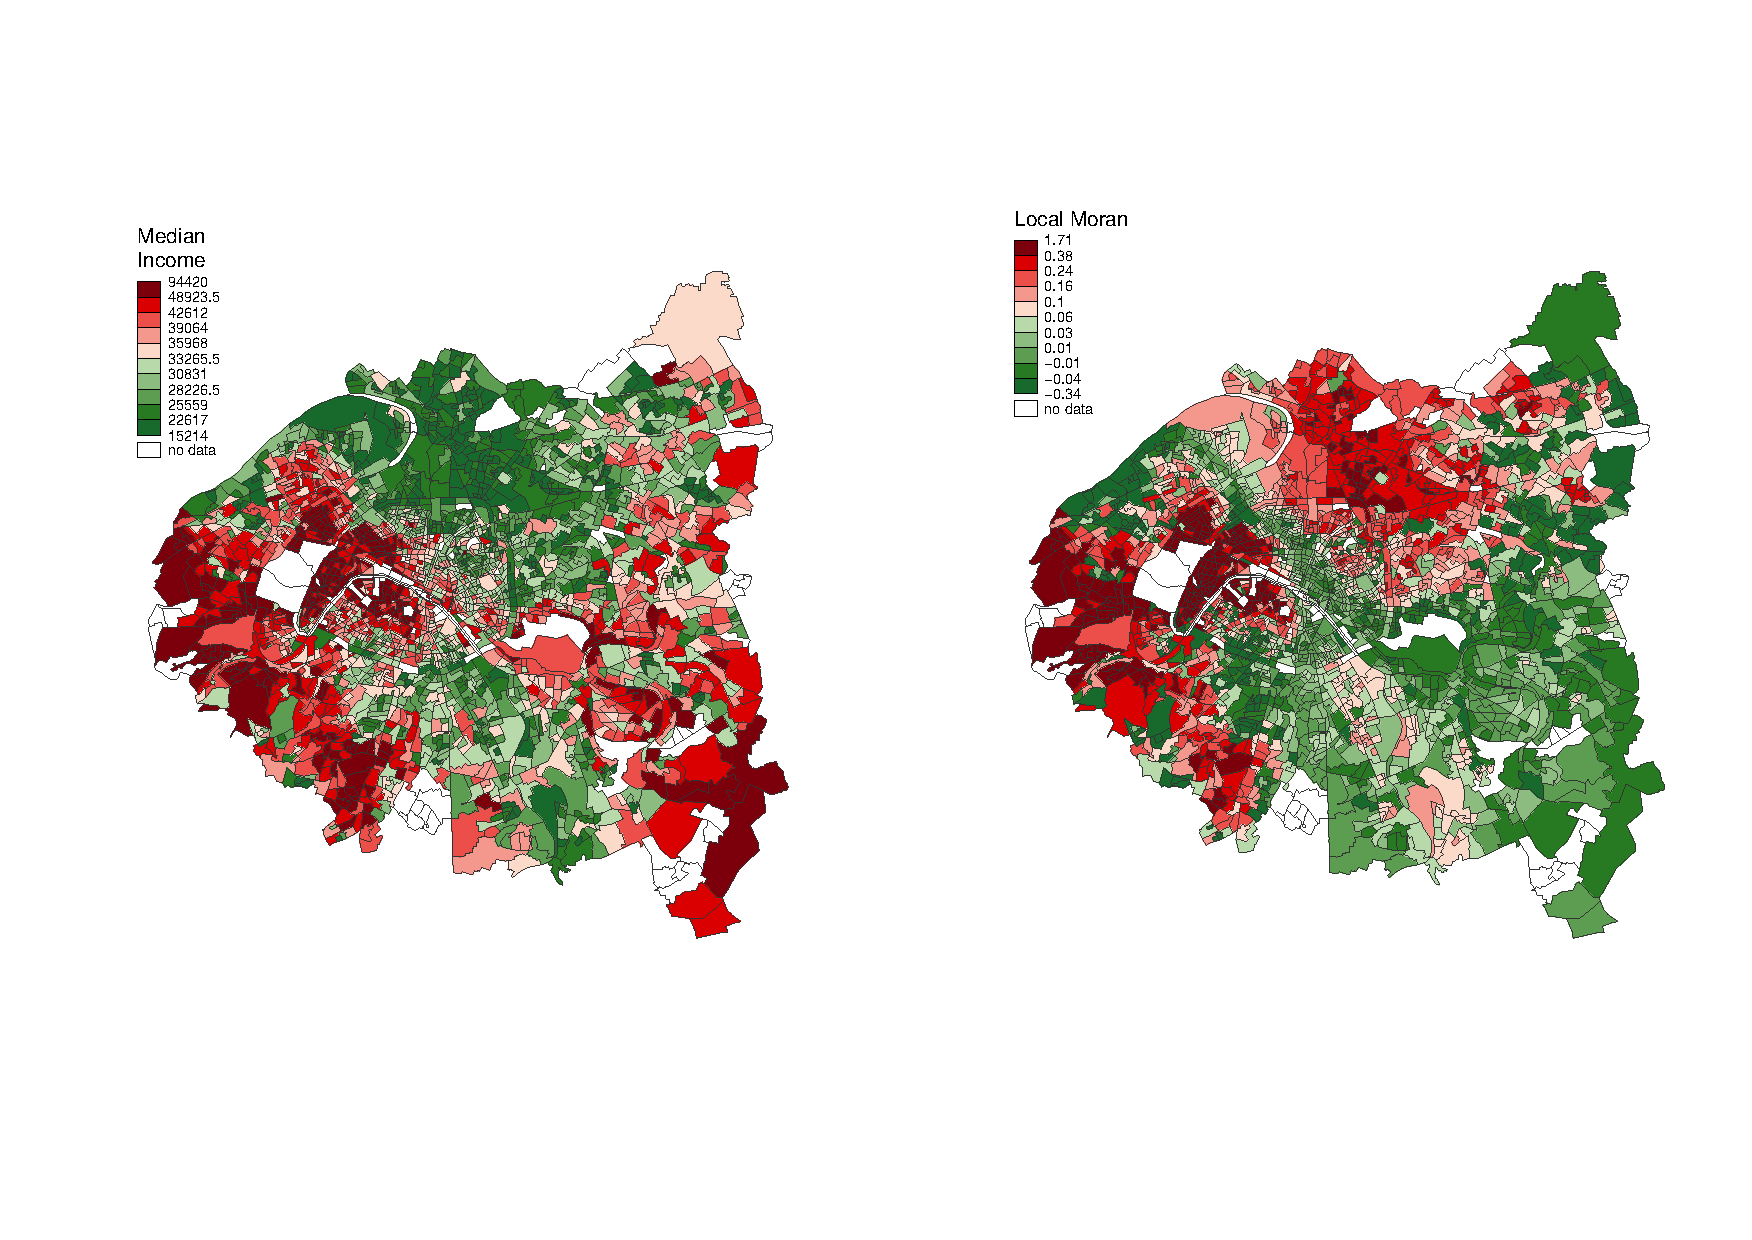
\includegraphics[width=1.2\textwidth]{Figures/RobustnessDiscrepancy/grandParis_income_moran.pdf}\hspace{-2cm}
\vspace{-2.5cm}
\caption[Maps of Metropolitan Segregation][Cartes de ségrégation métropolitaine]{\textbf{Maps of Metropolitan Segregation.} Maps show yearly median income on basic statistical units (IRIS) for the three departments constituting mainly the Great Paris metropolitan area, and the corresponding local Moran spatial autocorrelation index, defined for unit $i$ as $\rho_i = N/\sum_{j}w_{ij} \cdot \frac{\sum_{j} w_{ij} (X_j - \bar{X})(X_i - \bar{X})}{\sum_i (X_i - \bar{X})^2}$. The most segregated areas coincide with the richest and the poorest, suggesting an increase of segregation in extreme situations.}{\textbf{Cartes de ségrégation métropolitaine.} Les cartes montrent le revenu annuel médian pour les unités statistiques élémentaires (IRIS) pour les trois départements correspondant globalement à la métropole du Grand Paris, et l'index local d'autocorrelation spatiale de Moran correspondant, défini pour l'unité $i$ par $\rho_i = N/\sum_{j}w_{ij} \cdot \frac{\sum_{j} w_{ij} (X_j - \bar{X})(X_i - \bar{X})}{\sum_i (X_i - \bar{X})^2}$. Les zones les plus ségréguées coincident avec les plus riches et les plus pauvres, suggérant une augmentation de la ségrégation dans les cas extremes.}
\end{figure}
%%%%%%%%%%%%%%%%

\paragraph{Results}{Résultats}


\bpar{
We apply our method with these indicators on the Greater Paris area, constituted of four \emph{d{\'e}partements} that are intermediate administrative units. The recent creation of a new metropolitan governance system~\cite{gilli2009paris} underlines interrogations on its consistence, and in particular on its relation to intermediate spatial inequalities. We show in Fig. 1 maps of spatial distribution of median income and corresponding local index of autocorrelation. We observe the well-known West-East opposition and district disparities inside Paris as they were formulated in various studies, such as~\cite{guerois2009dynamique} through the analysis of real estate transactions dynamics. We then apply our framework to answer a concrete question that has implications for urban policy : \textit{how are the evaluation of segregation within different territories sensitive to missing data ?} To do so, we proceed to Monte Carlo simulations (75 repetitions) during which a fixed proportion of data is randomly removed, and the corresponding robustness index is evaluated with renormalized indicators. Simulations are done on each \emph{department} separately, each time relatively to the robustness of the evaluation of full Greater Paris. Results are shown in Fig. 2. All areas present a slightly better robustness than the reference, what could be explained by local homogeneity and thus more fiable segregation values. Implications for policy that can be drawn are for example direct comparisons between areas : a loss of 30\% of information on 93 area corresponds to a loss of only 25\% in 92 area. The first being a deprived area, the inequality is increased by this relative lower quality of statistical information. The study of standard deviations suggest further investigations as different response regimes to data removal seem to exist.
}{
La méthode est appliquée avec ces indicateurs à la zone du Grand Paris, constitué de 4 département qui sont des niveaux administratifs intermédiaires. La création récente d'un nouveau système de gouvernance métropolitaine~\cite{gilli2009paris} met en évidence des interrogations sur sa pertinence, notamment sur ses capacités d'atténuer les inégalités spatiales. On peut voir en Fig.~\ref{fig:segregmap} % TODO no fig label 
 les cartes de la distribution spatiale du revenu médian et de l'index local d'autocorrelation spatiale correspondant. La dichotomie bien connue entre est et ouest est retrouvée ainsi que la disparité des quartiers intra-muros, comme cela été présenté par diverses études, comme~\cite{guerois2009dynamique} à travers l'analyse des dynamiques des transactions immobilières. Notre cadre d'étude est ensuite appliqué à une question concrète ayant des implications pour la prise de décision : \textit{dans quelle mesure une évaluation de la ségrégation au sein de différents territoires est sensible aux données manquantes ?} Pour cela, on procède à des simulations de Monte-Carlo (75 répétitions) pour lesquelles une proportion fixe de données est supprimée aléatoirement, et l'indice de robustesse correspondant est évalué avec les indicateurs normalisés. Les simulations sont faites sur chaque département de façon indépendante, à chaque fois pour une robustesse relative à l'évaluation du Grand Paris complet. Les résultats sont présentés en Fig.~\ref{fig:missingdata}. Toutes les zones ont une robustesse légèrement meilleure que la référence, ce qui pourrait être expliqué par une homogénéité locale et donc des indices de ségrégation plus fiables. Les implications pour la prise de décision qui peuvent être par exemple tirées sont des comparaisons directes entre les zones : une perte de 30\% de l'information sur le 93 correspond à une perte de seulement 25\% pour le 92. La première zone étant déjà défavorisée socio-économiquement, l'inégalité est augmentée par cette qualité moindre de l'information statistique. L'étude des déviations standard suggère des études plus approfondies comme différents régimes de réponse à la suppression de données semblent exister.
}



%%%%%%%%%%%%%%%%
\begin{figure}
\centering
%\vspace{-1cm}
\hspace{-2cm}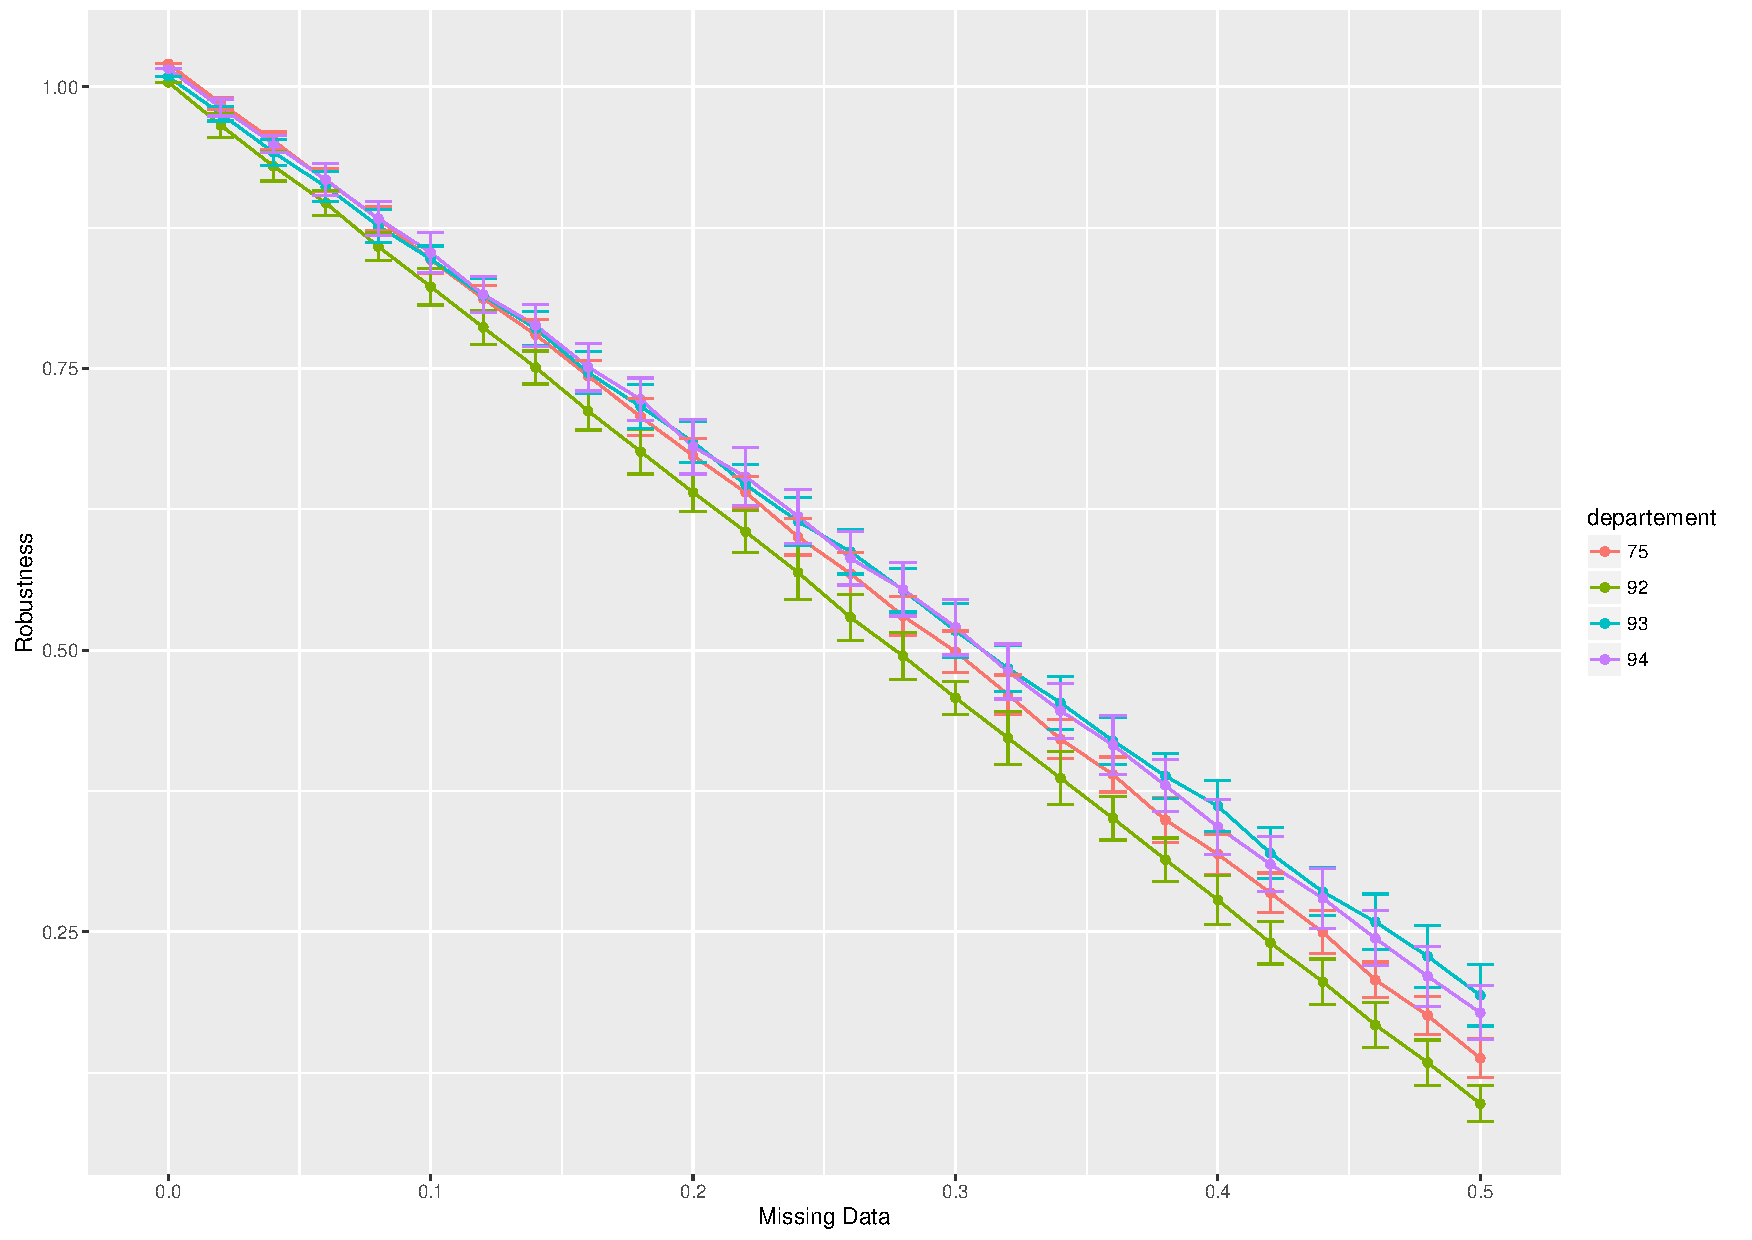
\includegraphics[width=0.55\textwidth]{Figures/RobustnessDiscrepancy/alldeps_rob_renormindics.pdf}
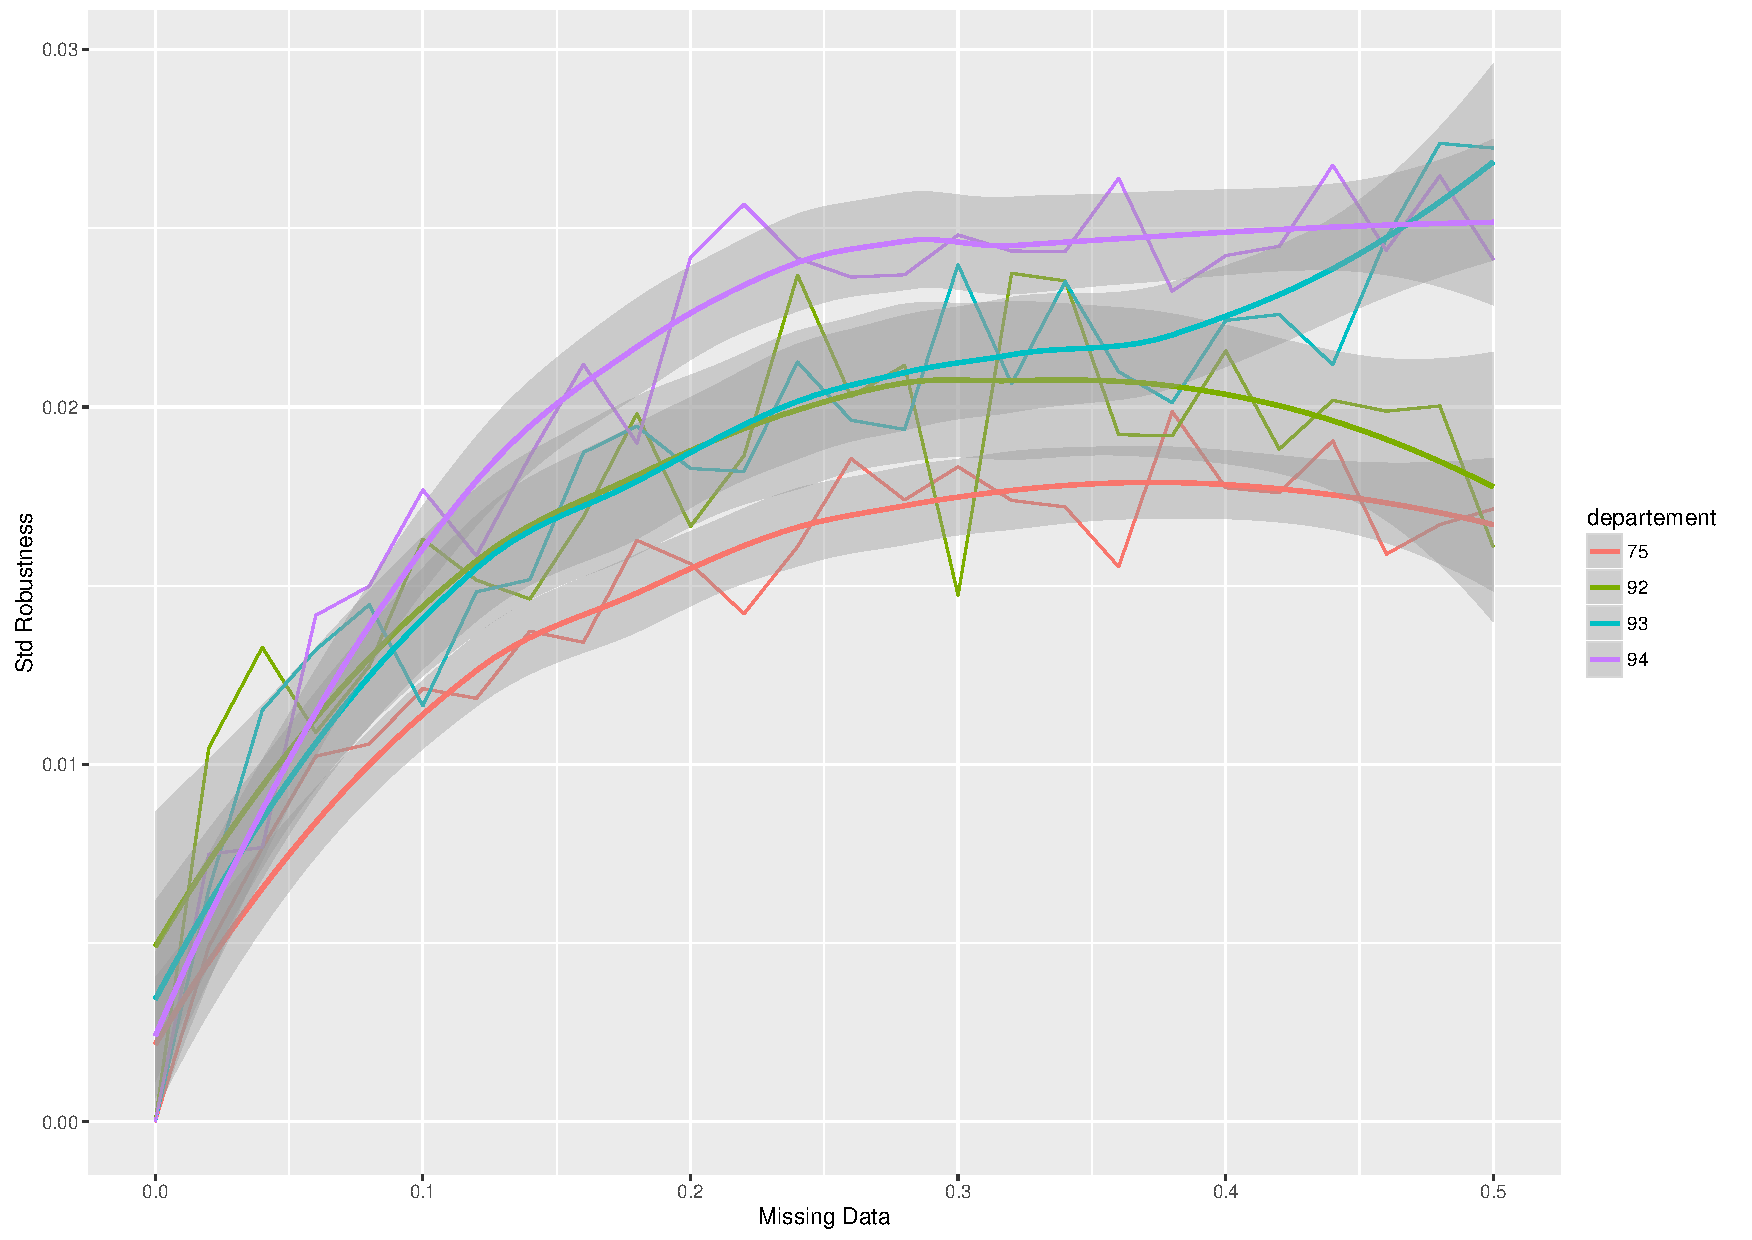
\includegraphics[width=0.55\textwidth]{Figures/RobustnessDiscrepancy/alldeps_robsd_renormindics.pdf}\hspace{-2cm}
\caption[Sensitivity of robustness to missing data][Sensibilité de la robustesse aux données manquantes]{\textbf{Sensitivity of robustness to missing data.} \textit{Left.} For each department, Monte Carlo simulations (N=75 repetitions) are used to determine the impact of missing data on robustness of segregation evaluation. Robustness ratios are all computed relatively to full metropolitan area with all available data. Quasi-linear behavior translates an approximative linear decrease of discrepancy as a function of data size. The similar trajectory of poorest departments (93,94) suggest the correction to linear behavior being driven be segregation patterns. \textit{Right.} Corresponding standard deviations of robustness ratios. Different regimes (in particular 93 against others) unveil phase transitions at different levels of missing data, meaning that the evaluation in 94 is from this point of view more sensitive to missing data.}{\textbf{Sensibilité de la robustesse aux données manquantes.} \textit{Gauche.} Pour chaque département, des simulations de Monte-Carlo (N=75 répétitions) sont utilisées pour déterminer l'impact des données manquantes sur la robustesse de l'évaluation de la ségrégation. Les ratios de robustesse sont tous calculés relativement à la région métropolitaine complète avec toutes les données disponibles. Le comportement quasi-linéaire traduit une décroissance approximativement linéaire de la discrépance en fonction de la taille des données. Les trajectoires similaires des départements les plus pauvres (93,94) suggère que la correction au comportement linéaire est fonction des motifs de ségrégation. \textit{Droite.} Déviations standard des ratios de robustesse. Les différents régimes (en particulier le 93 contre les autres) révèlent des transitions de phase à différents niveaux de données manquantes, signifiant que l'évaluation dans le 94 est de ce point de vue plus sensible aux données manquantes.}
% TODO typo département ?
\end{figure}
%%%%%%%%%%%%%%%%





%%%%%%%%%%%%%%%%
%% Discussion
%%%%%%%%%%%%%%%%
\subsection{Discussion}{Discussion}


%%%%%%%%%%%%%%%%
\subsubsection{Applicability to Real situations}{Applicabilité à des situations réelles}


\paragraph{Implications for Decision-making}{Implications pour la prise de décision}


\bpar{
The application of our method to concrete decision-making can be thought in different ways. First in the case of a comparative multi-attribute decision process, such as the determination of a transportation corridor, the identification of territories on which the evaluation may be flawed (i.e. has a poor relative robustness) could allow a more refined focus on these and a corresponding revision of datasets or an adapted revision of weights. In any case the overall decision-making process should be made more reliable. A second direction lays in the spirit of the real application we have proposed, i.e. the sensitivity of evaluation to various parameters such as missing data. If a decision appears as reliable because data have few missing points, but the evaluation is very sensitive to it, one will be more careful in the interpretation of results and taking the final decision. Further work and testing will however be needed to understand framework behavior in different contexts and be able to pilot its application in various real situations.
}{
L'application de notre méthode à des situations concrètes de prise de décision peu être pensée de différentes manières. Tout d'abord dans le cas d'un processus multi-attributs à but comparatif, comme la détermination d'un corridor pour une nouvelle infrastructure de transport, l'identification des territoires sur lesquels l'évaluation pourrait être biaisée (i.e. avec une mauvaise robustesse relative) devrait permettre une attention particulière pour ceux-ci, et l'adaptation des jeux de données ou la révision des points en conséquence. Dans tous les cas le processus total devrait être plus fiable. Une autre possibilité ressemble à l'application réelle que nous avons développé, i.e. la sensibilité de l'évaluation à divers paramètres comme les données manquantes. Si une décision parait fiable car la taille de données est grande, mais que l'évaluation est très sensible à la suppression de données, il faudra être prudent pour l'interprétation des résultats et pour la prise de décision finale. Un travail approfondi et de test sera cependant nécessaire pour comprendre le comportement du cadre dans différents contextes et pouvoir piloter son application dans des situations réelles diverses.
}


\paragraph{Integration Within Existing Frameworks}{Intégration au sein de cadres existants}


\bpar{
The applicability of the method on real cases will directly depend on its potential integration within existing framework. Beyond technical difficulties that will surely appear when trying to couple or integrate implementations, more theoretical obstacles could occur, such as fuzzy formulations of functions or data types, consistency issues in databases, etc. Such multi-criteria framework are numerous. Further interesting work would be to attempt integration into an open one, such as e.g. the one described in~\cite{tivadar2014oasis} which calculates various indices of urban segregation, as we have already illustrated the application on metropolitan segregation indexes.
}{
L'applicabilité de la méthode à des cas réels dépendra directement de son intégration potentielle dans des environnements existants. Au delà des difficultés techniques qui apparaissent nécessairement en essayant de coupler ou d'intégrer des implémentations existantes, des obstacles plus théoriques pourraient émerger, comme des formulations floues des fonctions ou des types de données, la cohérence des bases de données, etc. De tels cadres multi-critères sont nombreux. Un développement possible serait l'intégration dans un cadre open-source, comme par exemple celui décrit dans~\cite{tivadar2014oasis} qui calcule divers indices de ségrégation urbaine, comme on l'a déjà illustré pour l'application à la ségrégation métropolitaine.
}

\paragraph{Availability of Raw Data}{Disponibilité des données brutes}


\bpar{
In general, sensitive data such as transportation questionnaires, or very fine granularity census data are not openly available but provided already aggregated at a certain level (for instance French Insee Data are publicly available at basic statistical unit level or larger areas depending on variables and minimal population constraints, more precise data is under restricted access). It means that applying the framework may imply complicated data research procedure, its advantage to be flexible being thus reduced through additional constraints.
}{
De manière générale, des données sensibles comme des questionnaires de transport, ou des données de sondage à granularité très fine, ne sont pas disponibles de manière ouverte, mais fournis de manière déjà agrégée à un certain niveau (comme par exemple les données françaises de l'Insee sont disponibles publiquement au niveau des unités statistiques élémentaires ou pour des zones plus grandes selon les variables et des contraintes de population minimale, les données plus précises étant à accès restreint). Cela signifie que l'application de notre cadre peut impliquer une procédure de recherche de données laborieuse, l'avantage d'être flexible étant alors compensé par ces contraintes additionnelles.
}


%%%%%%%%%%%%%%%%
\subsubsection{Validity of Theoretical Assumptions}{Validité des hypothèses théoriques}


\bpar{
A possible limitation of our approach is the validity of the assumption formulating indicators as spatial integrals. Indeed, many socio-economic indicators are not necessarily depending explicitly on space, and trying to associate them with spatial coordinates may become a slippery slope (e.g. associate individual economic variables with individual residential coordinates will have a sense only if the use of the variable has a relation with space, otherwise it is a non-legitimate artifact). Even indicators which have a spatial value may derive from non-spatial variables, as~\cite{kwan1998space} points out concerning accessibility, when opposing integrated accessibility measures with individual-based non necessarily spatial-based (e.g. individual decisions) measures. Constraining a theoretical representation of a system to fit a framework by changing some of its ontological properties (always in the sense of real meaning of objects) can be understood as a violation of a fundamental rule of modeling and simulation in social science given in~\cite{banos2013HDR}, that is that there can be an universal ``language'' for modeling and some can not express some systems, having for consequence misleading conclusion due to ontology breaking in the case of an over-constrained formulation.
}{
Une limitation possible de notre approche est la validité de l'hypothèse qui formule les indicateurs comme des intégrales spatiales. En fait, de nombreux indicateurs socio-économiques ne dépendent pas nécessairement directement de l'espace, et essayer de les associer à des coordonnées peut entraîner sur une pente glissante (par exemple, associer des variables économiques individuelles à des coordonnées résidentielles aura un sens seulement si la variable à une relation à l'espace, autrement un devient un artefact superflu). Même des indicateurs qui ont une valeur spatiale peuvent dériver de variables non-spatiales, comme~ \cite{kwan1998space} le souligne au sujet de l'accessibilité, en opposant les mesures d'accessibilité intégrée aux mesures individu-centrées mais pas forcément basée sur l'espace (comme par exemple des décisions individuelles). Contraindre une représentation théorique d'un système pour le faire rentrer dans un cadre en changeant certaines de ses propriétés ontologiques (toujours dans le sens de la signification réelle des objets) peut être compris comme une violation d'une des règles pour la modélisation et la simulation en sciences sociales données par~\cite{banos2013HDR}, car cela impliquerait qu'il pourrait exister un langage universel pour la modélisation, malgré qu'il ne puisse retranscrire certains systèmes, ayant pour conséquences des conclusions errantes à cause d'une rupture d'ontologie dans le cas d'une formulation sur-contrainte.
}

%%%%%%%%%%%%%%%%
\subsubsection{Framework Generality}{Généralité du Cadre}


\bpar{
We argue that the fundamental advantage of the proposed framework is its generality and flexibility, since robustness of the evaluations are obtained only through data structure if ones relaxes constraints on the value of weight. Further work should go towards a more general formulation, suppressing for example the linear aggregation assumption. Non-linear aggregation functions would require however to present particular properties regarding integral inequalities. For example, similar results could search in the direction of integral inequalities for Lipschitzian functions such as the one-dimensional results of~\cite{dragomir1999ostrowski}.
}{
Nous soutenons qu'un des avantages fondamentaux de notre cadre est sa généralité et sa flexibilité, puisque la robustesse des évaluations est obtenue seulement par la structure des données si l'on relaxe les hypothèses sur les valeurs des poids. Des approfondissement pourraient inclure une formulation plus générale, en supprimant par exemple l'hypothèse d'agrégation linéaire. Des fonctions d'agrégation non-linéaires demanderaient toutefois de vérifier certaines propriétés regardant les inégalités intégrales. Par exemple, des résultats similaires pourraient être obtenus en s'orientant vers des inégalités intégrales pour fonctions Lipschitziennes, comme les résultats en une dimension de~\cite{dragomir1999ostrowski}.
}


%%%%%%%%%%%%%%%%
%% Conclusion
%%%%%%%%%%%%%%%%
\subsection*{Conclusion}{Conclusion}


\bpar{
We have proposed a model-independent framework to compare the robustness of multi-attribute evaluations between different urban systems. Based on data discrepancy, it provide a general definition of relative robustness without any assumption on model for the system, but with limiting assumptions that are the need of linear aggregation and of indicators being expressed through spatial kernel integrals. We propose a toy implementation based on real data for the city of Paris, numerical results confirming general expected behavior, and an implementation on real data for income segregation on Greater Paris metropolitan areas, giving possible insights into concrete policy questions. Further work should be oriented towards sensitivity analysis of the method, application to other real cases and theoretical assumptions relaxation, i.e. the relaxation of linear aggregation and spatial integration.
}{
Nous avons proposé un cadre indépendant du modèle pour comparer la robustesse d'évaluations multi-attributs entre différents systèmes urbains. A partir de la discrépance des données, on fournit une définition générale de la robustesse relative sans aucune hypothèse de modèle pour le système, mais en supposant une agrégation linéaire des objectifs et des indicateurs exprimés comme des intégrales à noyaux. Nous proposons une première implémentation preuve de concept pour la ville de Paris pour laquelle les résultats numériques confirment la tendance générale attendue, et une implémentation sur des données réelles pour la ségrégation de revenus pour la région métropolitaine du Grand Paris, fournissant des réponses possibles à des questions de prise de décision plus concrètes. Des développements possibles peuvent inclure une analyse de sensibilité de la méthode, des applications à d'autres cas réels et une relaxation des hypothèses théoriques, c'est à dire de l'agrégation linéaire et de l'intégration spatiale. % TODO confusion spatial/ kernel ? -> idem à l'oral ?
}


%\section*{Acknowledgments}

%The author would like to thank Julien Keutchayan (Ecole Polytechnique de Montr{\'e}al) for suggesting the original idea of using discrepancy, and anonymous reviewers for the useful comments and insights.




%%%%%%%%%%%%%%%%%%%%%%%%%%%%%




% quant epistemo after as a transition to more quanti part ?

%%%%%%%%%%%%%%%%%%%%%%%%%%%%%
% Chapter : Quantitative Epistemology


% Chapter 




\chapter{Quantitative Epistemology} % Chapter title

\label{ch:quantepistemo} % For referencing the chapter elsewhere, use \autoref{ch:name} 

%----------------------------------------------------------------------------------------


\headercit{something on knowledge}{}{}


A corollary of theoretical background proposed in chapter~\ref{ch:theory} is the need of an understanding of involved disciplines themselves to be able to build integrated heterogeneous models. The potentialities of couplings and integrations are greatly determined by existing approaches and corresponding gaps. This implies an advanced epistemological study in each field, that we propose to tackle in a systematic and quantitative way. This deliberate choice may shadow elaborated epistemological considerations but fits of purpose of preliminary investigations for the construction of models. 






%----------------------------------------------------------------------------------------


\newpage


\section{Algorithmic Systematic Review}


A broad bibliographical study suggests a scarcity of quantitative models of simulation integrating both network and urban growth. This absence may be due to diverging interests of concerned disciplines, resulting in a lack of communication.  We propose to proceed to an algorithmic systematic review to give quantitative elements of answer to this question. A formal iterative algorithm to retrieve corpuses of references from initial keywords, based on text-mining, is developed and implemented. We study its convergence properties and do a sensitivity analysis. We then apply it on queries representative of the specific question, for which results tend to confirm the assumption of disciplines compartmentalization.



\subsection{In search of models of co-evolution}


Transportation networks and urban land-use are known to be strongly coupled components of urban systems at different scales~\cite{bretagnolle2009organization}. One common approach is to consider them as co-evolving, avoiding misleading interpretations such as the myth of structural effect of transportation infrastructures~\cite{offner1993effets}. A question rapidly arising is the existence of models endogeneizing this co-evolution, i.e. taking into account simultaneous urban and network growth. We try to answer it using an algorithmic systematic review. We propose in this section, after a brief state of the art of existing literature, to present such an approach by formalizing the algorithm, which results are then presented and discussed. 

\subsection{Modeling Interactions between Urban Growth and Network Growth : An Overview}

\subsubsection{Land-Use Transportation Interaction Models.}

A wide class of models that have been developed essentially for planning purposes, which are the so-called Land-use Transportation Interaction Models, is a first type answering our research question. See recent reviews \cite{chang2006models}, \cite{iacono2008models} and \cite{wegener2004land} to get an idea of the heterogeneity of included approaches, that exist for more than 30 years. Recent models with diverse refinements are still developed today, such as \cite{delons:hal-00319087} which includes housing market for Paris area. Diverse aspects of the same system can be translated into many models (as \eg \cite{wegener1991one}), and traffic, residential and employment dynamics, resulting land-use evolution, influenced also by a static transportation network, are generally taken into account.

\subsubsection{Network Growth Approaches}

On the contrary, many economic literature has done the opposite of previous models, i.e. trying to reproduce network growth given assumptions on the urban landscape, as reviewed in \cite{zhang2007economics}. In~\cite{xie2009modeling}, economic empirical studies are positioned within other network growth approaches, such as work by physicists proposing model of geometrical network growth \cite{barthelemy2008modeling}. Analogy with biological networks was also done, reproducing typical robustness properties of transportation networks \cite{tero2010rules}.

\subsubsection{Hybrid Approaches}

Fewer approaches coupling urban growth and network growth can be found in the literature. \cite{barthelemy2009co} couples density evolution with network growth in a toy model. In~\cite{raimbault2014hybrid}, a simple Cellular Automaton coupled with an evolutive network reproduces stylized facts of human settlements described by Le Corbusier. At a smaller scale, \cite{achibet2014model} proposes a model of co-evolution between roads and buildings, following geometrical rules. These approaches stay however limited and rare.


\subsection{Bibliometric Analysis}

Literature review is a crucial preliminary step for any scientific work and its quality and extent may have a dramatic impact on research quality. Systematic review techniques have been developed, from qualitative review to quantitative meta-analyses allowing to produce new results by combining existing studies \cite{rucker2012network}. Ignoring some references can even be considered as a scientific mistake in the context of emerging information systems~\cite{lissacksubliminal}. We aim to take advantage of such techniques to tackle our issue.
Indeed, observing the form of the bibliography obtained in previous section raises some hypothesis. It is clear that all components are present for co-evolutive models to exist but different concerns and objectives seem to stop it. As it was shown by \cite{commenges:tel-00923682} for the concept of mobility, for which a ``small world of actors'' relatively closed invented a notion ad hoc, using models without accurate knowledge of a more general scientific context, we could be in an analog case for the type of models we are interested in. Restricted interactions between scientific fields working on the same objects but with different purposes, backgrounds and at different scales, could be at the origin of the relative absence of co-evolving models. 
While most of studies in bibliometrics rely on citation networks \cite{2013arXiv1310.8220N} or co-autorship networks \cite{2014arXiv1402.7268S}, we propose to use a less explored paradigm based on text-mining introduced in~\cite{chavalarias2013phylomemetic}, that obtain a dynamic mapping of scientific disciplines based on their semantic content. For our question, it has a particular interest, as we want to understand content structure of researches on the subject. We propose to apply an algorithmic method described in the following. The algorithm proceeds by iterations to obtain a stabilized corpus from initial keywords, reconstructing scientific semantic landscape around a particular subject.

\subsubsection{Description of the Algorithm}

Let $A$ be an alphabet, $A^{\ast}$ corresponding words and $T = \cup_{k\in \mathbb{N}} {A^{\ast}}^k$ texts of finite length on it. A reference is for the algorithm a record with text fields representing title, abstract and keywords. Set of references at iteration $n$ will be denoted $\mathcal{C} \subset T^3$. We assume the existence of a set of keywords $\mathcal{K}_n$, initial keywords being $\mathcal{K}_0$. An iteration goes as follows :

\begin{enumerate}
\item A raw intermediate corpus $\mathcal{R}_n$ is obtained through a catalog request providing previous keywords $\mathcal{K}_{n-1}$.
\item Overall corpus is actualized by $\mathcal{C}_n = \mathcal{C}_{n-1} \cup \mathcal{R}_n$.
\item New keywords $\mathcal{K}_n$ are extracted from corpus through Natural Language Processing treatment, given a parameter $N_k$ fixing the number of keywords.
\end{enumerate}

The algorithm stops when corpus size becomes stable or a user-defined maximal number of iterations has been reached. Fig. 1 shows the global workflow.



%%%%%%%%%%%%%%%%%%%%%%%%%%%%
\begin{figure}
\centering
\includegraphics[width=\textwidth]{Figures/PartI/QuantitativeEpistemo/schema_algo}
\caption[Systematic review algorithm workflow]{Global workflow of the algorithm, including implementation details : catalog request is done through Mendeley API ; final state of corpuses are RIS files.}
\label{fig:quantepistemo:algo}
\end{figure}
%%%%%%%%%%%%%%%%%%%%%%%%%%%%



%%%%%%%%%%%%%%%%%%%%%%%%%%%%
\subsubsection{Results}

\paragraph{Implementation}

Because of the heterogeneity of operations required by the algorithm (references organisation, catalog requests, text processing), it was found a reasonable choice to implement it in Java. Source code is available on the Github repository of the project1. Catalog request, consisting in retrieving a set of references from a set of keywords, is done using the Mendeley software API \cite{mendeley} as it allows an open access to a large database. Keyword extraction is done by Natural Language Processing (NLP) techniques, following the workflow given in \cite{chavalarias2013phylomemetic}, calling a Python script that uses \cite{bird2006nltk}.


\paragraph{Convergence and Sensitivity Analysis}

A formal proof of algorithm convergence is not possible as it will depend on the empirical unknown structure of request results and keywords extraction. We need thus to study empirically its behavior. Good convergence properties but various sensitivities to Nk were found as presented in Fig. 2. We also studied the internal lexical consistence of final corpuses as a function of keywords number. As expected, small number yields more consistent corpuses, but the variability when increasing stays reasonable.


%%%%%%%%%%%%%%%%%%%%%%%%%%%%
\begin{figure}
\centering
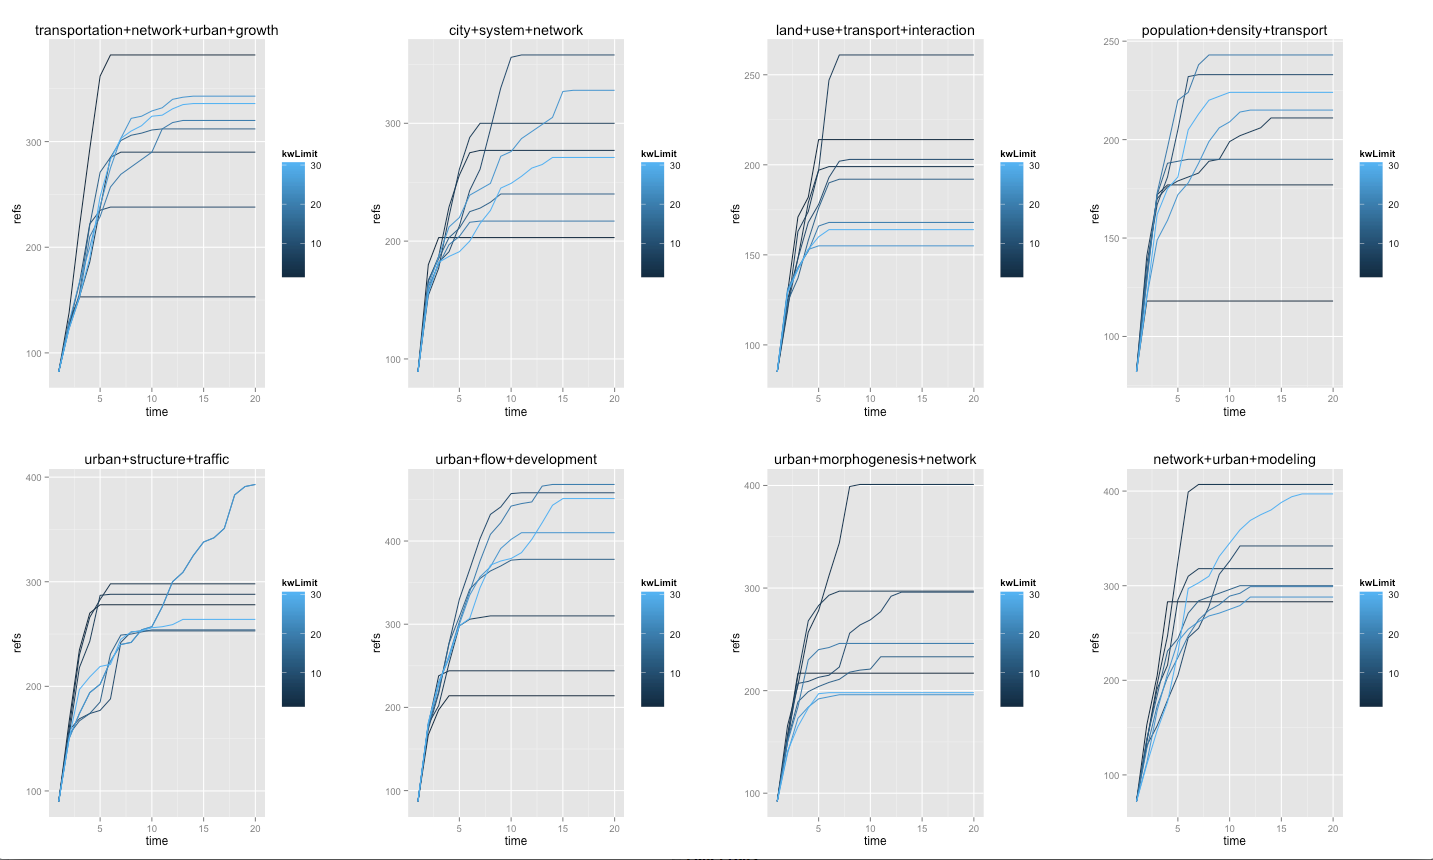
\includegraphics[width=\textwidth]{Figures/PartI/QuantitativeEpistemo/explo}
\medskip
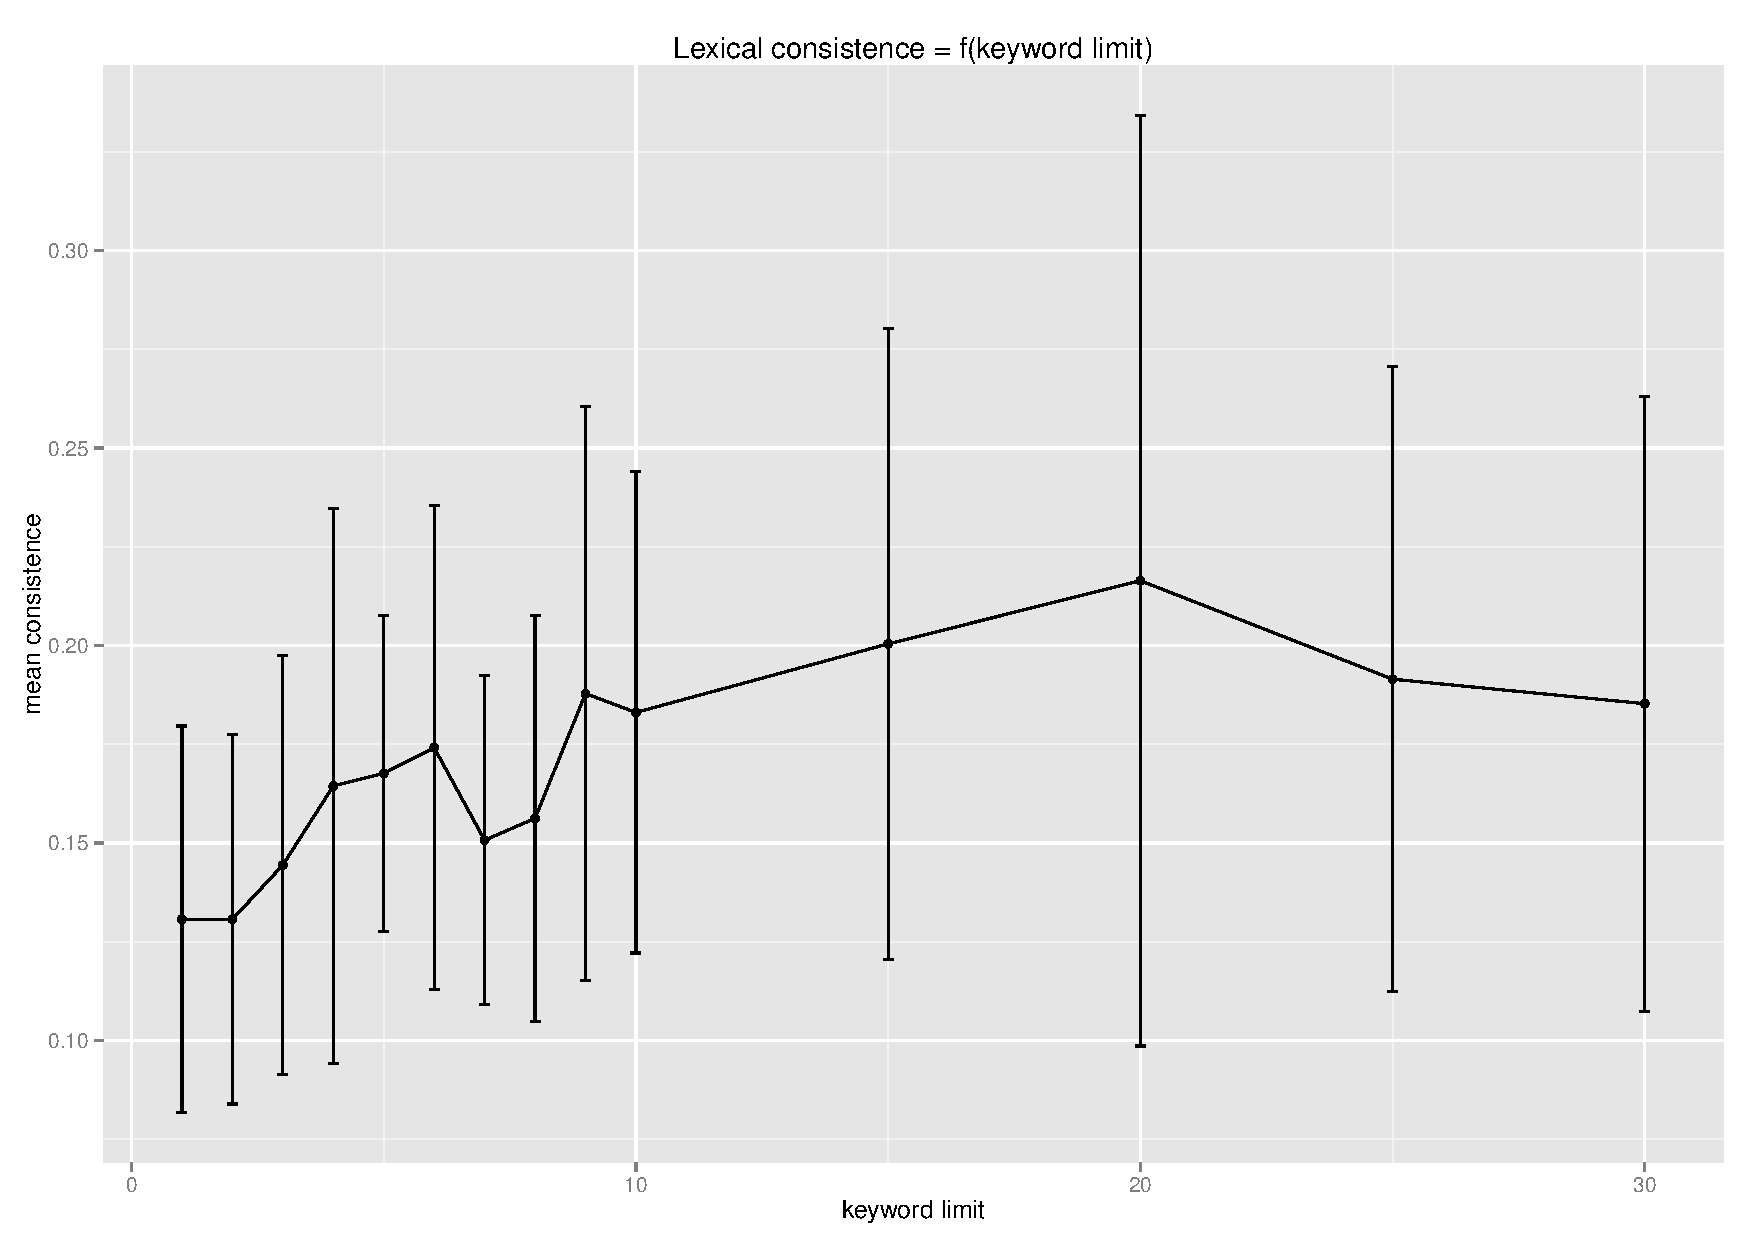
\includegraphics[width=0.8\textwidth]{Figures/PartI/QuantitativeEpistemo/lexicalConsistence_MeanSd}
\caption[Convergence and sensitivity analysis of systematic review algorithm]{Convergence and sensitivity analysis. Left : Plots of number of references as a function of iteration, for various queries linked to our theme (see further), for various values of $N_k$ (from 2 to 30). We obtain a rapid convergence for most cases, around 10 iterations needed. Final number of references appears to be very sensitive to keyword number depending on queries, what seems logical since encountered landscape should strongly vary depending on terms. Right : Mean lexical consistence and standard error bars for various queries, as a function of keyword number. Lexical consistence is defined though co-occurrences of keywords by, with $N$ final number of keywords, $f$ final step, and $c(i)$ co-occurrences in references, $k = \frac{2}{N(N-1)}\cdot \sum_{i,j \in \mathcal{K}_f}{\left| c(i) - c(j) \right|}$. The stability confirms the consistence of final corpuses.}
\label{fig:quantepistemo:sensitivity}
\end{figure}
%%%%%%%%%%%%%%%%%%%%%%%%%%%%




Once the algorithm is partially validated, we apply it to our question. We start from five different initial requests that were manually extracted from the various domains identified in the manual bibliography (that are ``city system network'', ``land use transport interaction'', ``network urban modeling'', ``population density transport'', ``transportation network urban growth''). We take the weakest assumption on parameter $N_k=100$, as it should less  constrain reached domains. After having constructed corpuses, we study their lexical distances as an indicator to answer our initial question. Large distances would go in the direction of the assumption made in section 2, i.e. that discipline self-centering may be at the origin of the lack of interest for co-evolutive models. We show in Table 1 values of relative lexical proximity, that appear to be significantly low, confirming this assumption.


\begin{table}
\centering
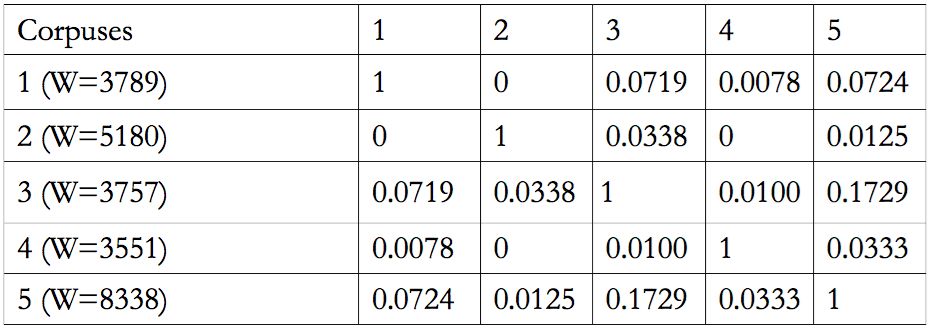
\includegraphics[width=\textwidth]{Figures/PartI/QuantitativeEpistemo/corpusesDistances}
\caption[Stationary lexical proximities]{Symmetric matrix of lexical proximities between final corpuses, defined as the sum of overall final keywords co-occurrences between corpuses, normalized by number of final keywords (100). We obtain very low values, confirming that corpuses are significantly far. Size of final corpuses is given as $W$.}
\end{table}



Further work is planned towards the construction of citation networks through an automatic access to Google Scholar that provides backward citations. The confrontation of inter-cluster coefficients on the citation network for the different corpuses with our lexical consistence results are an essential aspect of a further validation of our results.


The disturbing absence of models simulating the co-evolution of transportation networks and urban land-use, confirmed through a state-of-the-art covering many domain, may be due to the absence of communication between scientific disciplines studying different aspects of that problems. We have proposed an algorithmic method to give elements of answers through text-mining-based corpus extraction. First numerical results seem to confirm the assumption. However, such a quantitative analysis  should not be considered alone, but rather come as a back-up for qualitative studies that will be the object of further work, such as the one lead in~\cite{commenges:tel-00923682}, in which questionnaires with historical actors of modeling provide highly relevant information.





%--------------------------------------------------------------

\newpage

% Section describing cybergeo method.

\section{Refining bibliometrics through Hyper-network analysis}

%%%%%%%%%%%%%%
\subsection{Context}

As described before, semantic analysis does not contain all the information on disciplinary compartmentation nor on patterns of propagation of scientific knowledge as the ones contained in citation networks for example. Furthermore, data collection in the previous algorithm is subject to convergence towards self-consistent themes because of the proper structure of the method. It may give more insight about scientific social patterns of ontological choices in modeling to study communities in broader networks, that would more correspond to disciplines (or sub-disciplines depending on granularity level).

Previous works in quantitative epistemology using various types of networks have shown interesting potentialities. For the citation network, a good predicting power for citation patterns is for example obtained in~\cite{2013arXiv1310.8220N}. Co-authorship networks can also be used for predictive models~\cite{2014arXiv1402.7268S}. A multilayer network approach was recently proposed in~\cite{2016arXiv160106075O}, using bipartites networks of papers and scholars, in order to produce measures of interdisciplinarity. Disciplines can be stratified into layers to reveal communities between them and therein collaboration patterns~\cite{2015arXiv150601280B}.

\cite{10.1371/journal.pone.0147913}







%%%%%%%%%%%%%
\subsection{Application to a scientific journal}

\subsubsection{Presentation}

We briefly describe here an ongoing study that implemented the ideas given above for the particular case of a scientific journal for which bibliographical data is difficult to obtain, that is \texttt{cybergeo}, an electronic journal in theoretical and quantitative geography.


\cite{2015arXiv151003797G}
\cite{2016arXiv160208451P}
\cite{choi2014patent}
\cite{shibata2008detecting}


\subsubsection{Implementation}

The general architecture for data collection is presented in Fig.~\ref{fig:quantepistemo:data}. Citation data is collected from \texttt{Google Scholar}, that is the only source for incoming citations~\cite{noruzi2005google} in our case as the journal is not referenced in other databases. We are aware of the possible biaises using this single source~\cite{bohannon2014scientific}\footnote{or see \url{http://iscpif.fr/blog/2016/02/the-strange-arithmetic-of-google-scholars/}}, but these critics are more directed towards search results than citation counts. 



Text processing is done the same way as in previous section, expect that a particular treatment is done to language detection using \emph{stop-words} and a specific tagger \texttt{TreeTagger} is used for other languages than english~\cite{schmid1994probabilistic}.





%%%%%%%%%%%%%%%%%%
\begin{figure}
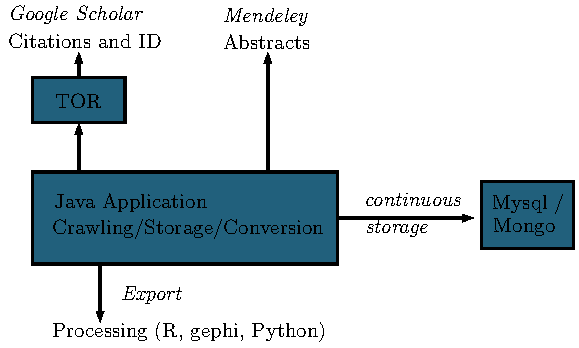
\includegraphics[width=\textwidth]{Figures/PartI/QuantitativeEpistemo/HyperNetwork/archi}
\caption[Heterogeneous Bibliographical Data Collection]{Heterogeneous Bibliographical Data Collection. Architecture of the application for content (semantic data), metadata and citation data collection.}
\label{fig:quantepistemo:data}
\end{figure}
%%%%%%%%%%%%%%%%%%


\subsubsection{Results}


We show in figures~\ref{fig:quantepistemo:citnw} and~\ref{fig:quantepistemo:semanticnw} preliminary results on citation and semantic network.

%%%%%%%%%%%%%%%%%
\begin{figure}
%\hspace{-3cm}
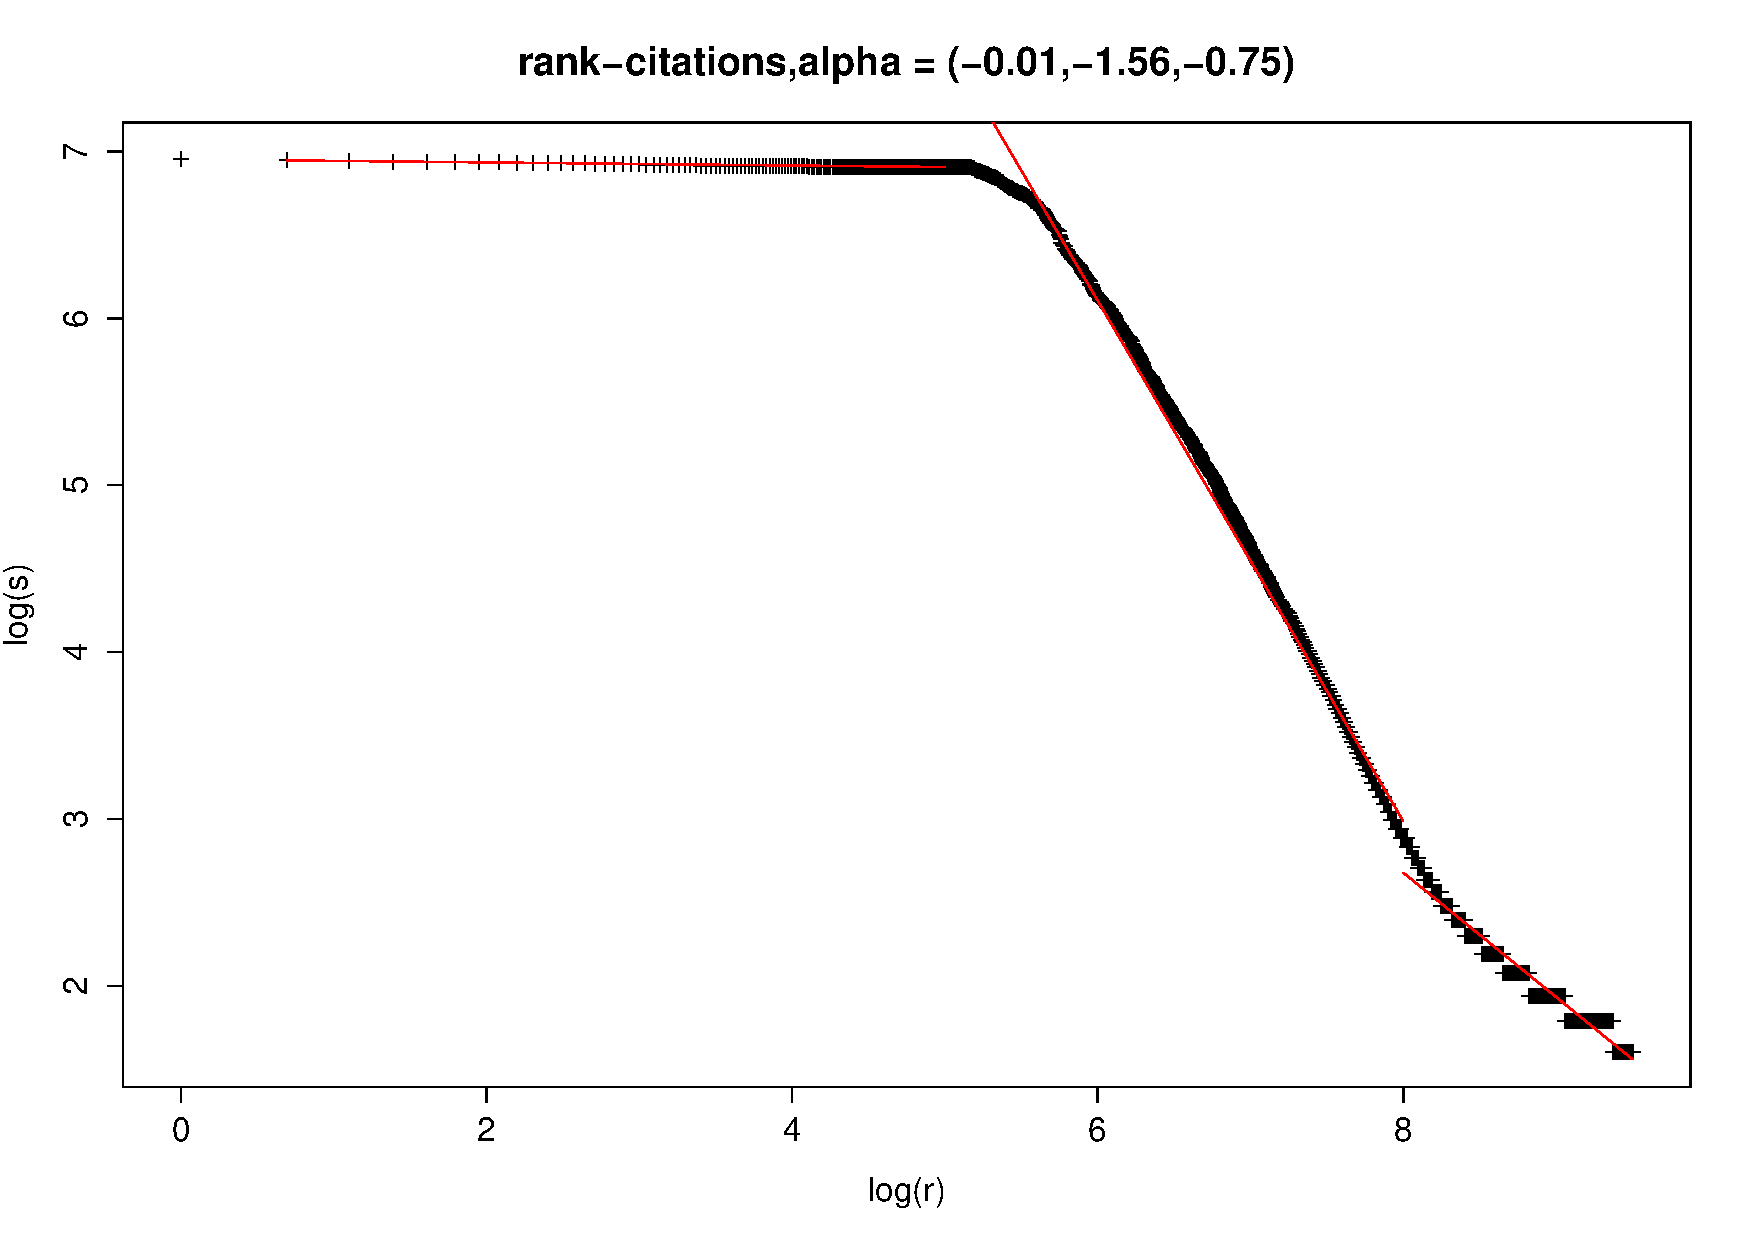
\includegraphics[width=\textwidth]{Figures/PartI/QuantitativeEpistemo/HyperNetwork/rank-size-all}
%\hspace{-3cm}
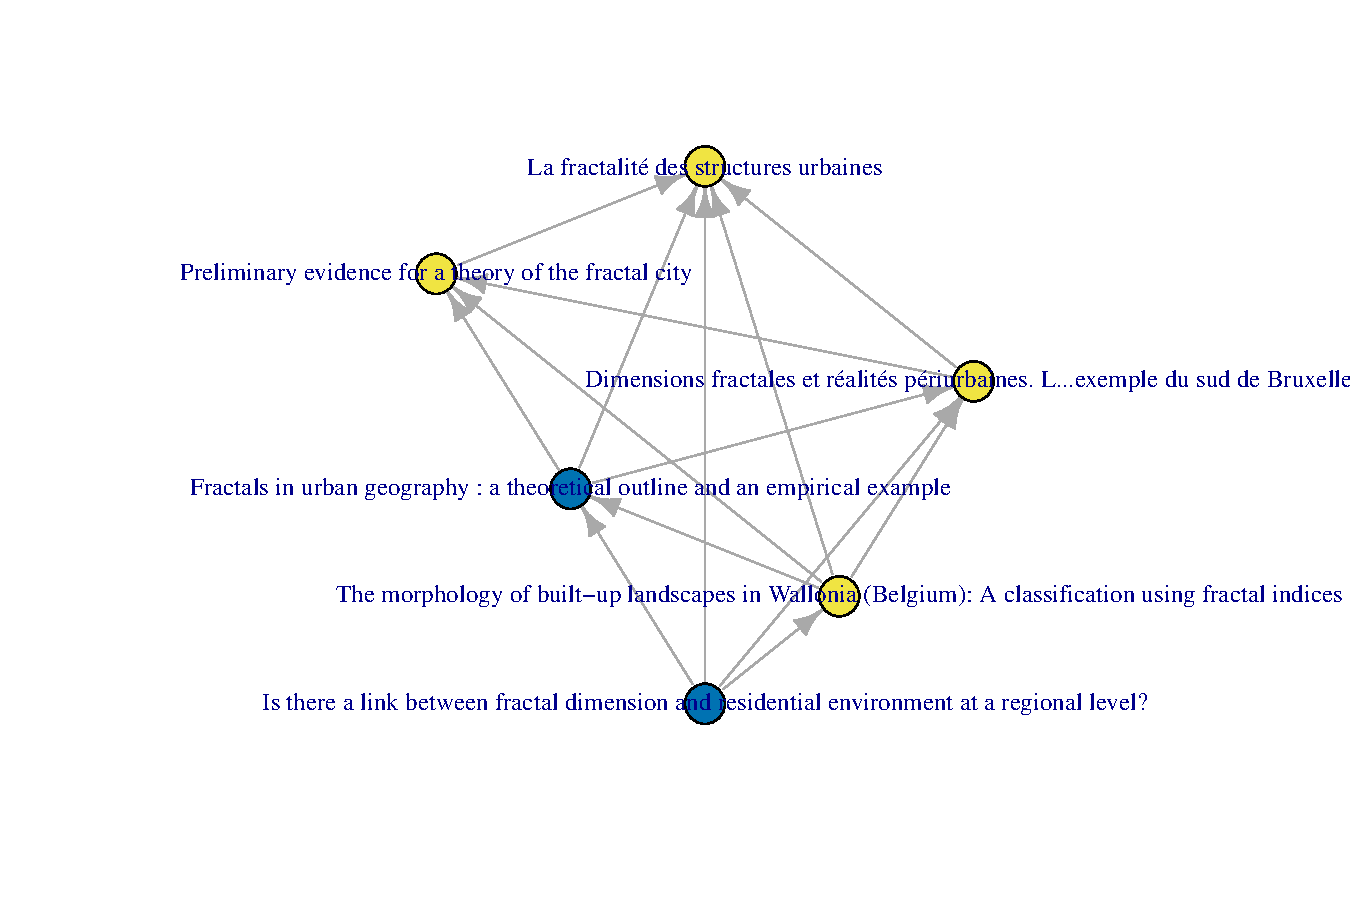
\includegraphics[width=\textwidth]{Figures/PartI/QuantitativeEpistemo/HyperNetwork/cybclic_2cyb_13761}
\caption[Properties of the citation network]{Properties of the citation network}
\label{fig:quantepistemo:citnw}
\end{figure}
%%%%%%%%%%%%%%%%%


%%%%%%%%%%%%%%%%%%
\begin{figure}
\hspace{-4cm}
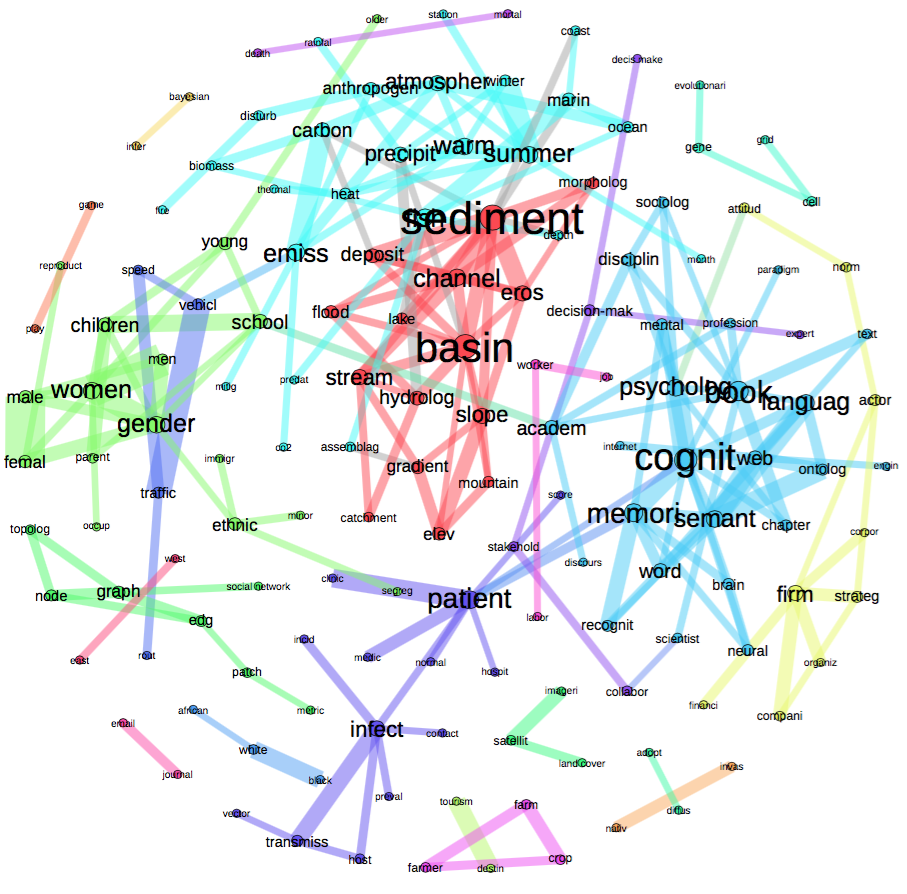
\includegraphics[width=1.4\textwidth]{Figures/PartI/QuantitativeEpistemo/HyperNetwork/all_lesslinks}
\caption[Semantic network of concepts in quantitative geography]{Semantic network of concepts in quantitative geography. Corpus consists of around $2\cdot 10^5$ abstracts of publications at a topological distance shorter than 2 from the journal \texttt{cybergeo} in the citation network. Relevance of keywords were estimated with the bootstrap method, }
\label{fig:quantepistemo:semanticnw}
\end{figure}
%%%%%%%%%%%%%%%%%%







%--------------------------------------------------------------

\newpage

%  Project section : describing ideas for more advanced text mining


\section{Towards modeling purpose and context automatic extraction}


A possible direction to strengthen our quantitative epistemological analysis would be to work on full textes related to the modeling of interaction between networks and territories, with the aim to automatically extract thematics within articles. The idea would be to perform some kind of automatized modelography, with possible features to be extracted that would be ontologies, model architecture or structures, scales, or even typical parameter values. It is not clear to what degree structure of models can be extracted from their description in papers and it surely depends on the discipline considered. For example in a framed field such as transportation planning, using a pre-defined ontology (in the sense of dictionary) and a fuzzy grammar could be efficient to extract information as the discipline is relatively formatted. In theoretical and quantitative geography, beyond the barrier of language, information organisation is surely less subject to unsupervised data-mining because of the more literary nature of the discipline : synonyms and style figures are generally the norm in good level human sciences writing, fuzzing a possible generic structure of knowledge description.

% cit LDA for thematic extraction ?









%%%%%%%%%%%%%%%%%%%%%%%%%%%%%





\cleardoublepage % Empty page before the start of the next part

%------------------------------------------------

\ctparttext{This part aims at producing knowledge from the empirical analysis of case studies and from first modeling experiments. Explicit testing of hypothesis drawn from the theory is not achieved yet as these are preliminary steps for a reasoned insight into empirical and modeling domains.} % Text on the Part 2 page describing the content in Part 2


% Part II : Empirical analysis / Toy-modeling
% TODO : part 2 should set up the elementary bricks for further work ?
%\part{Modeling and Empirical Analysis} % Second part of the thesis
%\part{Architecture and Building Bricks : preparing the construction}
\part{Materials}




%%%%%%%%%%%%%%%
% Transportation Equilibrium
%  -> first insight at a micro scale, from empirical point of view


% Chapter 

%\bchapter{Investigating the Empirical Existence of Static User Equilibrium}{
%Investigation Empirique de l'Existence de l'Equilibre Utilisateur Statique
%} % Chapter title
\chapter{Investigating the Empirical Existence of Static User Equilibrium}


\label{ch:transportation}

% NOTE : wont stay a chapter 

%----------------------------------------------------------------------------------------


\bpar{
The Static User Equilibrium is a powerful framework for the theoretical study of traffic. Despite the restricting assumption of stationary flows that intuitively limit its application to real traffic systems, many operational models implementing it are still used without an empirical validation of the existence of the equilibrium. We investigate its existence on a traffic dataset of three months for the region of Paris, FR. The implementation of an application for interactive spatio-temporal data exploration allows to hypothesize a high spatial and temporal heterogeneity, and to guide further quantitative work. The assumption of locally stationary flows is invalidated in a first approximation by empirical results, as shown by a strong spatial and temporal variability in shortest paths and in network topological measures such as betweenness centrality. Furthermore, the behavior of spatial autocorrelation index of congestion patterns at different spatial ranges suggest a chaotic evolution at the local scale, especially during peak hours. We finally discuss the implications of these empirical findings and describe further possible developments based on the estimation of Lyapunov dynamical stability of traffic flows.
}{
L'Equilibre Utilisateur Statique est un cadre puissant pour l'étude théorique du trafic. Malgré l'hypothèse restreignante de stationnarité des flots qui intuitivement limite son application aux systèmes de trafic réels, de nombreux modèles opérationnels qui l'implémentent sont toujours utilisés sans validation empirique de l'existence de l'équilibre. Nous étudions celle-ci sur un jeu de données de trafic couvrant trois mois sur la région parisienne. L'implémentation d'une application d'exploration interactive de données spatio-temporelles permet de formuler l'hypothèse d'une forte hétérogénéité spatiale et temporelle, guidant les études quantitatives. L'hypothèse de flots localement stationnaires est invalidée en première approximation par les résultats empiriques, comme le montrent une forte variabilité spatio-temporelle des plus courts chemins et des mesures topologiques du réseau comme la centralité de chemin. De plus, le comportement de l'index d'autocorrelation spatiale pour les motifs de congestion à différentes portées spatiales suggère une évolution chaotique à l'échelle locale, en particulier lors des heures de pointe. Nous discutons finalement les implications de ces résultats empiriques et proposons des possibles développements futurs basés sur l'estimation de la stabilité dynamique au sens de Lyapounov des flots de trafic.
}


%%%%%%%%%%%%%%%%%%%%%%%
%\bsection{Introduction}{Introduction}
\section{Introduction}
\label{treq:introduction}


\bpar{
Traffic Modeling has been extensively studied since seminal work by~\cite{wardrop1952road} : economical and technical elements at stake justify the need for a fine understanding of mechanisms ruling traffic flows at different scales. Many approaches with different purposes coexist today, of which we can cite dynamical micro-simulation models, generally opposed to equilibrium-based techniques. Whereas the validity of micro-based models has been largely discussed and their application often questioned, the literature is relatively poor on empirical studies assessing the stationary equilibrium assumption in the Static User Equilibrium (SUE) framework. Various more realistic developments have been documented in the literature, such as Dynamic Stochastic User Equilibrium (DSUE) (see e.g. a description by~\cite{han2003dynamic}). An intermediate between static and stochastic frameworks is the Restricted Stochastic User Equilibrium, for which route choice sets are constrained to be realistic (\cite{rasmussen2015stochastic}). Extensions that incorporate user behavior with choice models have more recently been proposed, such as~\cite{zhang2013dynamic} taking into account both the influence of road pricing and congestion on user choice with a Probit model. Relaxations of other restricting assumptions such as pure user utility maximization have been also introduced, such as the Boundedly Rational User Equilibrium described by~\cite{mahmassani1987boundedly}. In this framework, user have a range of satisfying utilities and equilibrium is achieved when all users are satisfied. It produces more complex features such as the existence of multiple equilibria, and allows to account for specific stylized facts such as irreversible network change as developed by~\cite{guo2011bounded}. Other models for traffic assignment, inspired from other fields have also recently been proposed : in~\cite{puzis2013augmented}, an extended definition of betweenness centrality combining linearly free-flow betweenness with travel-time weighted betweenness yield a high correlation with effective traffic flows, acting thus as a traffic assignment model. It provides direct practical applications such as the optimization of traffic monitors spatial distribution.
}{
La modélisation du trafic a été largement étudiée depuis les travaux séminaux de Wardrop (\cite{wardrop1952road}) : les enjeux économiques et techniques justifient entre autre le besoin d'une compréhension fine des mécanismes régissant les flots de trafic à différentes échelles. Différentes approches aux objectifs différents coexistent aujourd'hui, parmi lesquels on trouve par exemple les modèles dynamiques de micro-simulation, généralement opposés aux techniques de basant sur l'équilibre. Tandis que la validité des modèles microscopiques a été étudiée de façon conséquente et leur application souvent questionnée, la littérature est relativement pauvre en études empiriques assurant l'hypothèse d'équilibre stationnaire du cadre de l'Equilibre Utilisateur Statique (EUS). De nombreux développements plus réalistes on été documentés dans la littérature, tels l'Equilibre Utilisateur Dynamique Stochastique (EUDS) (voir pour une description par example~\cite{han2003dynamic}). A un niveau intermédiaire entre les cadres statiques et stochastiques se trouve l'Equilibre Utilisateur Stochastique Restreint, pour lequel les choix d'itinéraire des utilisateurs sont contraints à un ensemble d'alternatives réalistes (\cite{rasmussen2015stochastic}). D'autres extensions prenant en compte le comportement de l'utilisateur via des modèles de choix ont été proposé plus récemment, comme~\cite{zhang2013dynamic} qui inclut à la fois l'influence de la tarification routière et de la congestion sur le choix avec un modèle Probit. La relaxation d'autres hypothèses restrictives comme la maximisation pure de l'utilité par l'utilisateur ont aussi été introduites, tels l'Equilibre Utilisateur Borné décrit par~\cite{mahmassani1987boundedly}. Dans ce cadre, l'utilisateur est satisfait si son utilité tombe dans un intervalle et l'équilibre est achevé lorsque chaque utilisateur est satisfait. Les dynamiques résultantes sont plus complexes comme révélé par l'existence d'équilibres multiples, et permet de rendre compte de faits stylisés spécifiques comme des évolutions irréversibles du réseau comme développé par~\cite{guo2011bounded}. D'autres modèles d'attribution de trafic inspirés d'autres domaines ont également été plus récemment proposés: dans~\cite{puzis2013augmented}, une définition étendue de la centralité de chemin qui combine linéairement le centralité des flots non-contraints avec une centralité pondérée par le temps de parcours permet d'obtenir une forte corrélation avec les flots de trafic effectifs, fournissant ainsi un modèle d'attribution de trafic. Cela fournit également des applications pratiques comme l'optimisation de la distribution spatiale des capteurs de trafic.
}

\bpar{
Despite all these developments, some studies and real-world applications still rely on Static User Equilibrium. Parisian region e.g. uses a static model (MODUS) for traffic management and planning purposes. \cite{leurent2014user} introduce a static model of traffic flow including parking cruising and parking lot choice: it is legitimate to ask, specifically at such small scales, if the stationary distribution of flows is a reality. An example of empirical investigation of classical assumptions is given in~\cite{zhu2010people}, in which revealed route choices are studied. Their conclusions question ``Wardrop’s first principle'' implying that users choose among a well-known set of alternatives. In the same spirit, we investigate the possible existence of the equilibrium in practice. More precisely, SUE assumes a stationary distribution of flows over the whole network. This assumption stays valid in the case of local stationarity, as soon as time scale for parameter evolution is considerably greater than typical time scales for travel. The second case which is more plausible and furthermore compatible with dynamical theoretical frameworks, is here tested empirically. 
}{
Malgré ces nombreux développements, de nombreuses études et applications concrètes se reposent toujours sur l'Equilibre Utilisateur Statique. La région parisienne utilise par exemple un modèle statique (MODUS) pour gérer et planifier le trafic. \cite{leurent2014user} introduit un modèle statique de flots qui inclut les recherches locales et le choix du parking : il est légitime de s'interroger, en particulier à de si faibles échelles, si la stationnarité de la distribution des flots est une réalité. Une example d'exploration empirique des hypothèses classiques est donné par~\cite{zhu2010people}, pour lequel les choix d'itinéraires révélés sont étudiés. Les conclusions questionnent le ``premier principe de Wardrop'' qui implique que les utilisateurs choisissent parmi un ensemble d'alternatives parfaitement connu. Dans le même esprit, nous étudions l'existence possible de l'équilibre en pratique. Plus précisément, l'EUS suppose une distribution stationnaire des flots sur l'ensemble du réseau. Cette hypothèse reste valable dans le cas d'une stationnarité locale, tant que l'échelle temporelle d'évolution des paramètres est considérablement plus grande que les échelles typiques de voyage. Le second cas qui est plus plausible et de plus compatible avec les cadres théoriques dynamiques est testé ici.
}


\bpar{
The rest of the paper is organized as follows : data collection procedure and dataset are described ; we present then an interactive application for the interactive exploration of the dataset aimed to give intuitive insights into data patterns ; we present then results of various quantitative analyses that give convergent evidence for the non-stationarity of traffic flows ; we finally discuss implications of these results and possible developments.
}{
La suite de ce travail s'organise ainsi : la procédure de collection de données ainsi que le jeu de données sont décrits ; nous présentons ensuite une application interactive pour l'exploration du jeu de données, dans le but de fournir une intuitions sur les motifs présents ; puis nous donnons divers résultats d'analyses quantitatives allant dans le sens d'indices convergents pour une non-stationnarité des flots de trafic ; nous discutons finalement les implications de ces résultats et des développements possibles.
}



%%%%%%%%%%%%%%%%%%%%%
%\section{\bpar{Data collection}{Collecte des données}}
\section{Data collection}

%%%%%%%%%%%%%%%%%%%%%
%\subsection{\bpar{Dataset Construction}{Construction du jeu de données}}
\subsection{Dataset Construction}


\bpar{
We propose to work on the case study of Parisian Metropolitan Region. An open dataset was constructed for highway links within the region, collecting public real-time open data for travel times (available at www.sytadin.fr). As stated by~\cite{bouteiller2013open}, the availability of open datasets for transportation is far to be the rule, and we contribute thus to a data opening by the construction of our dataset. Our data collection procedure consists in the following simple steps, executed each two minutes by a \texttt{python} script :
\begin{itemize}
\item fetch raw webpage giving traffic information
\item parse html code to retrieve traffic links id and their corresponding travel time
\item insert all links in a \texttt{sqlite} database with the current timestamp.
\end{itemize}
}{
Nous proposons de travailler sur l'étude de cas de la région métropolitaine de Paris. Un jeu de données ouvert a été construit, comprenant les liens autoroutiers dans la région, par collecte des données publiques en temps réel des temps de parcours (disponible sur www.sytadin.fr). Comme rappelé par~\cite{bouteiller2013open}, la disponibilité de jeux de données ouverts pour les transports est loin d'être la règle, et nous contribuons ainsi à une ouverture par la construction de notre jeu de données. La procédure de collecte de données consiste en les points suivants, executés toutes les deux minutes par un script \texttt{python} :
\begin{itemize}
\item récupération de la page web brute donnant les informations de trafic
\item parsing du code html afin de récupérer les identifiants des liens de trafic et les temps de parcours correspondants
\item insertion des liens dans une base \texttt{sqlite} avec le temps courant.
\end{itemize}
}


\bpar{
The automatized data collection script continues to enrich the database as time passes, allowing future extensions of this work on a larger dataset and a potential reuse by scientists or planners. The latest version of the dataset is available online (sqlite format) under a Creative Commons License\footnote{at \texttt{http://37.187.242.99/files/public/sytadin{\_}latest.sqlite3}}.
}{
Le script automatisé de collection des données continue d'enrichir la base au fur et à mesure du temps, permettant des développements futurs de ce travail sur un jeu de données plus large, et une réutilisation potentielle pour des travaux scientifiques ou opérationnels. La dernière version du jeu de données au format sqlite est disponible en ligne sous une Licence \emph{Creative Commons}\footnote{à l'adresse \texttt{http://37.187.242.99/files/public/sytadin{\_}latest.sqlite3}}.
}


%%%%%%%%%%%%%%%%%%%%%
%\bsubsection{Data Summary}{Description des données}
\subsection{Data Summary}


\bpar{
A time granularity of 2 minutes was obtained for a three months period (February 2016 to April 2016 included). Spatial granularity is in average 10km, as travel times are provided for major links. The dataset contains 101 links. Raw data we use is effective travel time, from which we can construct travel speed and relative travel speed, defined as the ratio between optimal travel time (travel time without congestion, taken as minimal travel times on all time steps) and effective travel time. Congestion is constructed by inversion of a simple BPR function with exponent 1, i.e. we take $c_i = 1 - \frac{t_{i,min}}{t_i}$ with $t_i$ travel time in link $i$ and $t_{i,min}$ minimal travel time.
}{
Une granularité de deux minutes a été obtenue pour une période de trois mois (de février 2016 à avril 2016 inclus. La granularité spatiale est en moyenne de 10km, les temps de trajet étant fournis pour les liens majeurs. Le jeu de données contient 101 liens. La variable brute utilisée est le temps de trajet effectif, à partir duquel il est possible de construire la vitesse de trajet et la vitesse relative de trajet, définie comme le rapport entre temps de trajet optimal (temps de trajet sans congestion, pris comme le temps minimal sur l'ensemble des pas de temps) et le temps de trajet effectif. La congestion est construite par inversion d'un fonction BPR simple avec exposant 1, i.e. en prenant $c_i = 1 - \frac{t_{i,min}}{t_i}$ avec $t_i$ temps de trajet effectif dans le lien $i$ et $t_{i,min}$ temps de trajet minimal.
}



%%%%%%%%%%%%%%%%%%%%%%
%\section{\bpar{Methods and Results}{Méthodes and Résultats}}
\section{Methods and Results}


%%%%%%%%%%%%%%%%%%%%%%
%\subsection{\bpar{Visualization of spatio-temporal congestion patterns}{Visualisation des motifs spatio-temporels de congestion}}
\subsection{Visualization of spatio-temporal congestion patterns}

\bpar{
As our approach is fully empirical, a good knowledge of existing patterns for traffic variables, and in particular of their spatio-temporal variations, is essential to guide any quantitative analysis. Taking inspiration from an empirical model validation literature, more precisely Pattern-oriented Modeling techniques introduced by~\cite{grimm2005pattern}, we are interested in macroscopic patterns at given temporal and spatial scales: the same way stylized facts are in that approach extracted from a system before trying to model it, we need to explore interactively data in space and time to find relevant patterns and associated scales. We implemented therefore an interactive web-application for data exploration using \texttt{R} packages \texttt{shiny} and \texttt{leaflet}\footnote{source code for the application and analyses is available on project open repository at\\
\texttt{https://github.com/JusteRaimbault/TransportationEquilibrium}}.
It allows dynamical visualization of congestion among the whole network or in a particular area when zoomed in. The application is accessible online at \texttt{http://shiny.parisgeo.cnrs.fr/transportation}. A screenshot of the interface is presented in Figure~\ref{fig:fig-1}. Main conclusion from interactive data exploration is that strong spatial and temporal heterogeneity is the rule. The temporal pattern recurring most often, peak and off-peak hours is on a non-negligible proportion of days perturbed. In a first approximation, non-peak hours may be approximated by a local stationary distribution of flows, whereas peaks are too narrow to allow the validation of the equilibrium assumption. Spatially we can observe that no spatial pattern is clearly emerging. It means that in case of a validity of static user equilibrium, meta-parameters ruling its establishment must vary at time scales smaller than one day. We argue that traffic system must in contrary be far-from-equilibrium, especially during peak hours when critical phase transitions occur at the origin of traffic jams. 
}{
Notre approche étant entièrement empirique, une bonne connaissance des motifs existants pour les variables de traffic, en particulier de leur variations spatio-temporelles, est crucial pour guider toute analyse quantitative. En s'inspirant de la littérature étudiant la validation empirique de modèles, plus précisément les techniques de \emph{Modélisation orientée-motifs} introduites par~\cite{grimm2005pattern}, nous nous intéressons au motifs macroscopiques à des échelles temporelles et spatiales données : d'une manière équivalente aux faits stylisés qui sont dans cette approches extraits d'un système avant de tenter de le modéliser, nous devons explorer les données de manière interactive dans le temps et l'espace afin d'identifier des motifs pertinents et les échelles associées. Une application web interactive a ainsi été implémentée pour explorer les données, à l'aide des packages \texttt{R} \texttt{shiny} et \texttt{leaflet}\footnote{le code source de l'application et des analyses est disponible sur le dépôt ouvert du projet à\\
\texttt{https://github.com/JusteRaimbault/TransportationEquilibrium}}.
Cela permet une visualisation dynamique des motifs de congestion sur l'ensemble du réseau ou dans une zone particulière grace au zoom. L'application est accessible en ligne à l'adresse \texttt{http://shiny.parisgeo.cnrs.fr/transportation}. La Figure~\ref{fig:fig-1} présente une capture d'écran de l'interface. La conclusion majeure de l'exploration interactive des données est qu'une grande hétérogénéité spatiale et temporelle est la règle. Le motif temporel le plus récurrent, la périodicité journalière des heures de pointe, est perturbée pour une proportion non négligeable de jours. En première approximation, les heures creuses peuvent être approchées par une distribution localement stationnaire des flots, tandis que les heures de pointe sont trop courtes pour pouvoir impliquer la validation de l'hypothèse d'équilibre. Concernant l'espace, aucun motif spatial particulier n'émerge clairement. Cela signifie que dans le cas d'une validité de l'équilibre utilisateur statique, les méta-paramètres régissant son établissement doivent varier à des échelles temporelles plus courtes qu'un jour. Nous postulons au contraire que le système de traffic est loin de l'équilibre, en particulier pendant les heures de pointe pendant lesquelles des transitions de phase critiques à l'origine des embouteillages émergent.
}
 


%%%%%%%%%%%%%%%%%%
\begin{figure}
\vspace{1cm}
\centering
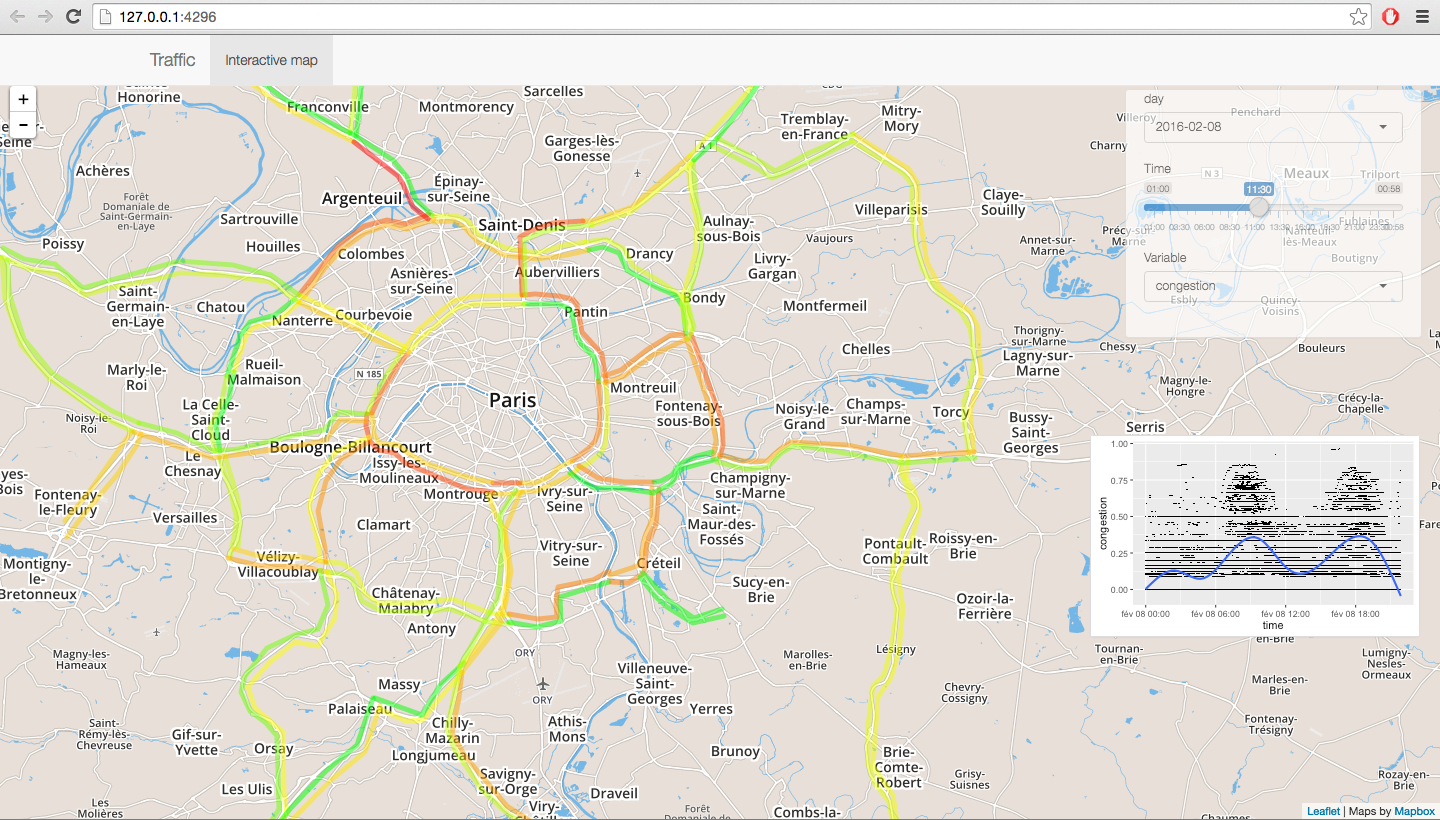
\includegraphics[width=\textwidth]{Figures/TransportationEquilibrium/gr1}
\caption{}
%\caption{\bpar{Capture of the web-application to explore spatio-temporal traffic data for Parisian region. It is possible to select date and time (precision of 15min on one month, reduced from initial dataset for performance purposes). A plot summarizes congestion patterns on the current day.}{Capture de l'application web permettant l'exploration spatio-temporelle des données de traffic pour la région Parisienne. Il est possible de choisir date et heure (précision de 15min sur un mois, réduite par rapport au jeu de données initial pour des raisons de performance). Un graphe résume les motifs de congestion pour la journée courante.}}
\label{fig:fig-1}
\end{figure}
%%%%%%%%%%%%%%%%%%



%%%%%%%%%%%%%%%%%%%%%%%%
%\subsection{\bpar{Spatio-temporal Variability of Travel Path}{Variabilité Spatio-temporelle des Trajets}}
\subsection{Spatio-temporal Variability of Travel Path}

\bpar{
Following interactive exploration of data, we propose to quantify the spatial variability of congestion patterns to validate or invalidate the intuition that if equilibrium does exist in time, it is strongly dependent on space and localized. The variability in time and space of travel-time shortest paths is a first way to investigate flow stationarities from a game-theoretic point of view. Indeed, the static User Equilibrium is the stationary distribution of flows under which no user can improve its travel time by changing its route. A strong spatial variability of shortest paths at short time scales is thus evidence of non-stationarity, since a similar user will take a few time after a totally different route and not contribute to the same flow as a previous user. Such a variability is indeed observed on a non-negligible number of paths on each day of the dataset. We show in Figure~\ref{fig:fig-2} an example of extreme spatial variation of shortest path for a particular Origin-Destination pair.
}{
A la suite de l'exploration interactive des données, nous proposons de quantifier la variabilité spatiale des motifs de congestion pour valider ou invalider l'intuition que si l'équilibre existe par rapport au temps, il est fortement dépendant de l'espace et localisé. La variabilité spatio-temporelle des plus courts chemins de trajet est une première façon d'étudier la stationnarité des flots d'un point de vue de théorie des jeux. En effet, l'Equilibre Utilisateur Statique est la distribution stationnaire des flots sous laquelle aucun utilisateur ne peut augmenter son temps de trajet en changeant son itinéraire. Une forte variabilité spatiale des plus courts chemins sur de courtes échelles spatiales révèle ainsi une non-stationnarité, puisque un même utilisateur prendra un chemin complètement différent après un court laps de temps et ne contribuera plus au même flot que précédemment. Une telle variabilité est en effet observée sur un nombre non-négligeable de chemins pour chaque jour du jeu de données. La figure~\ref{fig:fig-2} montre un exemple de variation spatiale extrême d'un trajet pour une paire Origine-Destination particulière.
}

\bpar{
The systematic exploration of travel time variability across the whole dataset, and associated travel distance, confirms, as described in Figure 3, that travel time absolute variability has often high values of its maximum across OD pairs, up to 25 minutes with a temporal local mean around 10min. Corresponding spatial variability produces detours up to 35km.
}{
L'exploration systématique de la variabilité du temps de trajet sur l'ensemble du jeu de données, et des distances de trajet associées, confirme, comme présenté en figure~\label{fig:fig-3}, que la variation absolue du temps de trajet présente fréquemment une forte variation de son maximum sur l'ensemble des paires O-D, jusqu'à 25 minutes avec une moyenne temporelle locale autour de 10 minutes. La variabilité spatiale correspondante entraine des détours allant jusqu'à 35km.
}


%%%%%%%%%%%%%%%%%%%
\begin{figure}
\centering
\vspace{1.5cm}
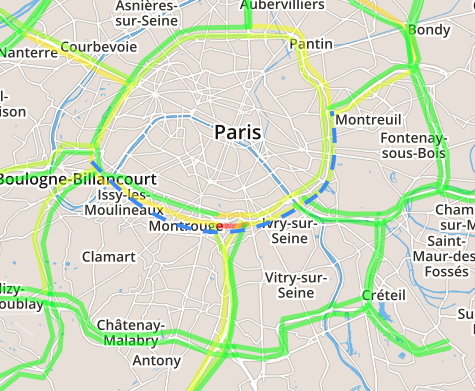
\includegraphics[width=0.47\textwidth]{Figures/TransportationEquilibrium/gr21}\hfill
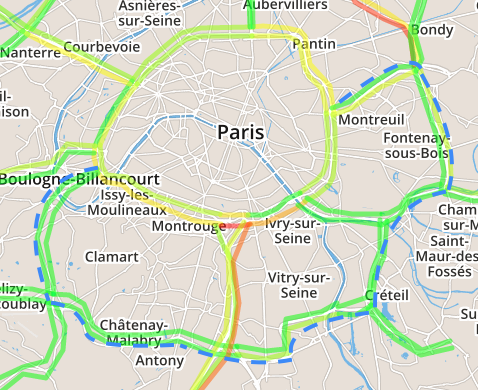
\includegraphics[width=0.47\textwidth]{Figures/TransportationEquilibrium/gr22}
\caption{}
%\bcaption{Spatial variability of travel-time shortest path (shortest path trajectory in dotted blue). In an interval of only 10 minutes, between 11/02/2016 00:06 (left) and 11/02/2016 00:16 (right), the shortest path between \emph{Porte d'Auteuil} (West) and \emph{Porte de Bagnolet} (East), increases in effective distance of $\simeq 37$km (with an increase in travel time of only 6min), due to a strong disruption on the ring of Paris.}{Variabilité spatiale d'un plus court chemin en temps de trajet (trajet du plus court chemin en pointillé bleu). Dans un intervalle de seulement 10 minutes, entre le 11/02/2016 00:06 (à gauche) et le 11/02/2016 00:16 (à droite), le plus court chemin entre Porte d'Auteuil à l'ouest et Porte de Bagnolet à l'est, augmente en distance effective de $\simeq 37$km (avec une augmentation du temps de trajet de seulement 6 minutes), à cause d'une forte perturbation sur le périphérique parisien.}
\label{fig:fig-2}
\end{figure}
%%%%%%%%%%%%%%%%%%%



%%%%%%%%%%%%%%%%%%%
\begin{figure}[t]\vspace*{4pt}
\centering
\centerline{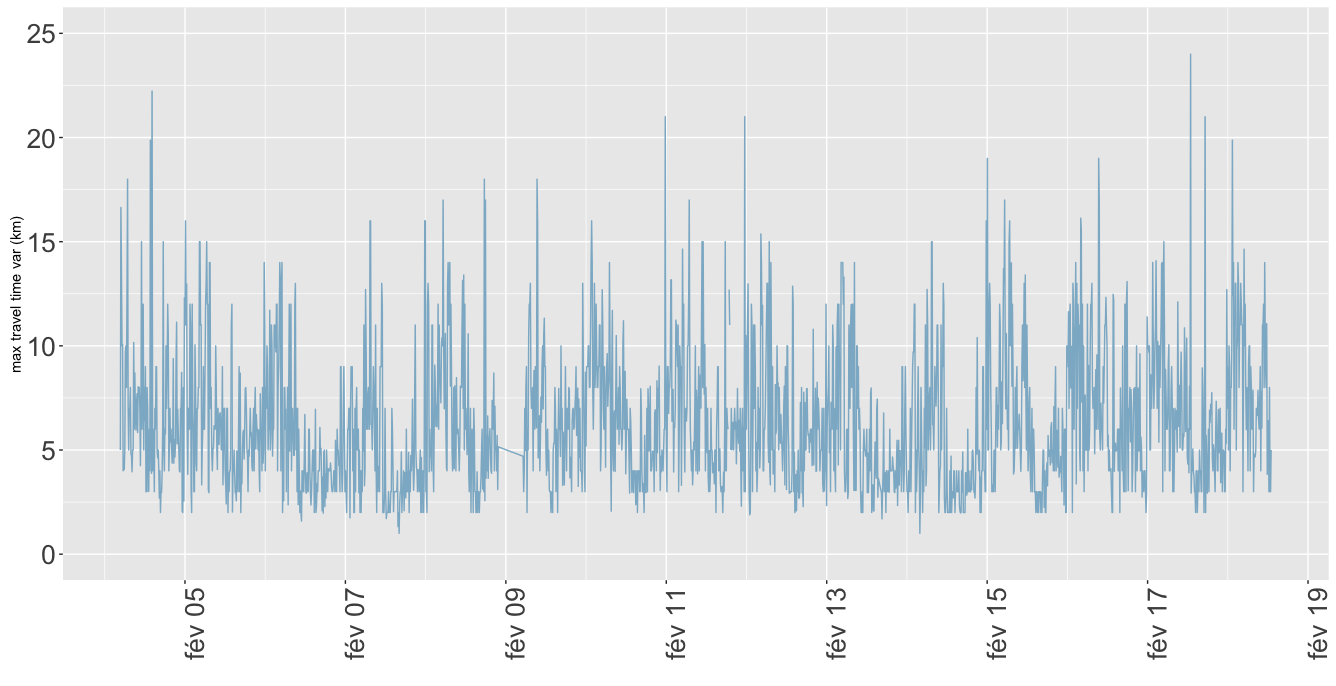
\includegraphics[width=0.8\textwidth]{Figures/TransportationEquilibrium/gr31}}
\centerline{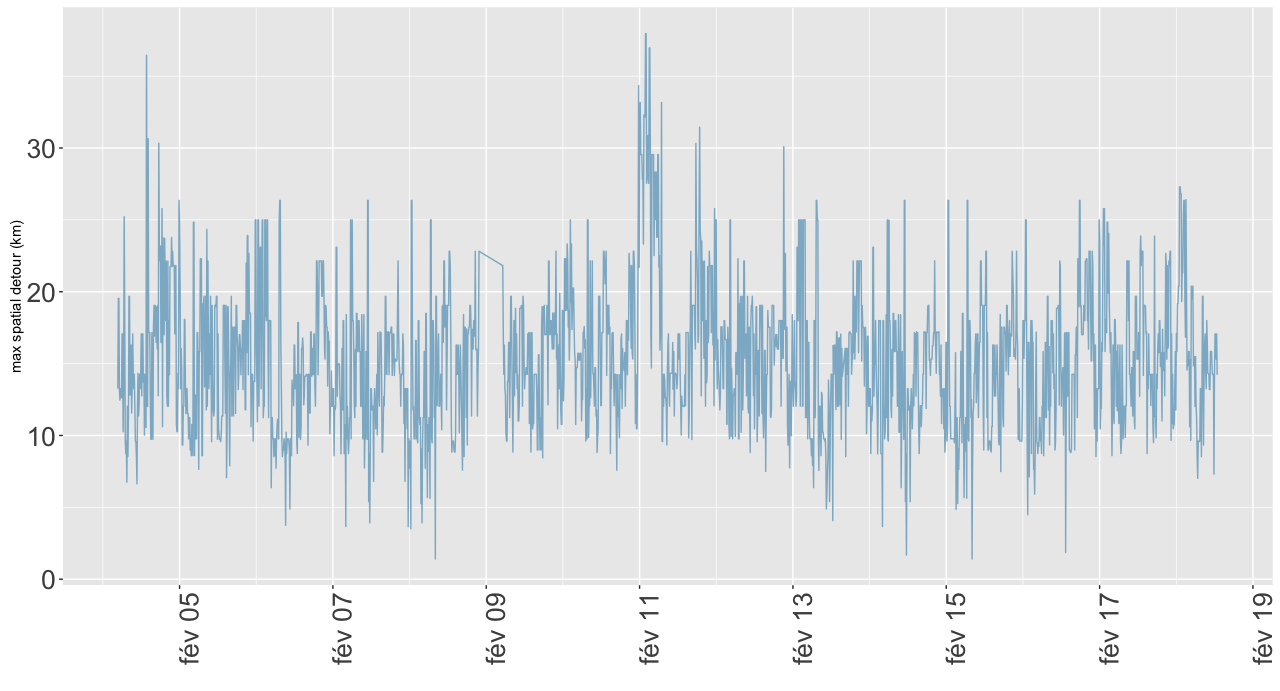
\includegraphics[width=0.8\textwidth]{Figures/TransportationEquilibrium/gr32}}
\caption{}
%\caption{\bpar{Travel time (top) in min and corresponding travel distance (bottom) maximal variability on a two weeks sample. We plot the maximal on all OD pairs of the absolute variability between two consecutive time steps. Peak hours imply a high time travel variability up to 25 minutes and a path length variability up to 35km.}{Variabilité maximale du temps de trajet (en haut) en minutes et de la distance de trajet correspondante (en bas) pour un échantillon de deux semaines. Le graphe représente le maximum sur l'ensemble des paires Origine-Destination de la variabilité absolue entre deux pas de temps consécutifs. Les heures de pointe induisent une forte variabilité du temps de trajet, allant jusqu'à 25 minutes et une variabilité de distance jusqu'à 35km.}}
\label{fig:fig-3}
\end{figure}
%%%%%%%%%%%%%%%%%%%




%%%%%%%%%%%%%%%%%%%
\subsection{Stability of Network measures} % Stabilité des mesures de réseau

\bpar{
The variability of potential trajectories observed in the previous section can be confirmed by studying the variability of network properties. In particular, network topological measures capture global patterns of a transportation network. Centrality and node connectivity measures are classical indicators in transportation network description as recalled in~\cite{bavoux2005geographie}. The transportation literature has developed elaborated and operational network measures, such as network robustness measures to identify critical links and measure overall network resilience to disruptions (an example among many is the Network Trip Robustness index introduced in~\cite{sullivan2010identifying}).
}{
La variabilité des trajectoires potentielles observée dans la section précédente peu être confirmée par l'étude de la variabilité des propriétés du réseau. En particulier, les mesures topologiques de réseau capturent les motifs globaux dans un réseau de transport. Les mesures de centralité et de connectivité des noeuds sont des indicateurs classiques pour la description des réseaux de transport comme rappelé par~\cite{bavoux2005geographie}. La littérature en transports a développé des mesures de réseau élaborées et opérationnelles, comme des mesures de robustesse pour identifier les liens critiques et mesurer la résilience globale du réseau aux perturbations (un exemple parmi d'autres est l'indice de \emph{Robustesse du Réseau Effective} introduit dans ~\cite{sullivan2010identifying}).
}



\bpar{
More precisely, we study the betweenness centrality of the transportation network, defined for a node as the number of shortest paths going through the node, i.e. by the equation

%%%%%%%%%%%%%%%
% equation betweeness
\begin{equation}
b_i = \frac{1}{N(N-1)}\cdot \sum_{o\neq d \in V}\mathbbm{1}_{i\in p(o\rightarrow d)}
\end{equation}
%%%%%%%%%%%%%%%

where $V$ is the set of network vertices of size $N$, and $p(o\rightarrow d)$ is the set of nodes on the shortest path between vertices o and d (the shortest path being computed with effective travel times). This index is more relevant to our purpose than other measures of centrality such as closeness centrality that does not include potential congestion as betweenness centrality does.
}{
Plus précisément, nous étudions la centralité de chemin du réseau de transport, défini pour un noeud comme le nombre de plus courts chemins passant par celui-ci, i.e. par l'équation

%%%%%%%%%%%%%%%
% equation betweeness
\begin{equation}
b_i = \frac{1}{N(N-1)}\cdot \sum_{o\neq d \in V}\mathbbm{1}_{i\in p(o\rightarrow d)}
\end{equation}
%%%%%%%%%%%%%%%

où $V$ est l'ensemble des sommets du réseau de taille $N$, et $p(o\rightarrow d)$ est l'ensemble des noeuds sur le plus court chemin entre les sommets $o$ et $d$ (le plus court chemin étant calculé avec le temps de trajet effectif). Cette mesure de centralité est plus adaptée que d'autre dans notre cas, comme la centralité de proximité qui n'inclut pas la congestion potentielle comme la centralité de chemin.
}



\bpar{
We show in Figure 4 the relative absolute variation of maximal betweenness centrality for the same time window than previous empirical indicators. More precisely we plot the value of

%%%%%%%%%%%%%%%
% eq relative variability
\begin{equation}
\Delta b(t) = \frac{\left|\max_i (b_i(t + \Delta t)) - \max_i (b_i(t))\right|}{\max_i (b_i(t))}
\end{equation}
%%%%%%%%%%%%%%%



where $\Delta t$ is the time step of the dataset (the smallest time window on which we can capture variability). This absolute relative variation has a direct meaning : a variation of 20\% (which is attained a significant number of times as shown in Fig.~\ref{fig:fig-4}) means that in case of a negative variation, at least this proportion of potential travels have changed route and the local potential congestion has decrease of the same proportion. In the case of a positive variation, a single node has captured at least 20\% of travels. Under the assumption (that we do not try to verify in this work and assume to be also not verified as shown by~\cite{zhu2010people}, but that we use as a tool to give an idea of the concrete meaning of betweenness variability) that users rationally take the shortest path and assuming that a majority of travels are realized such a variation in centrality imply a similar variation in effective flows, leading to the conclusion that they can not be stationary in time (at least at a scale larger than $\Delta t$) nor in space.
}{
Nous montrons en Figure 4 la variation relative absolue du maximum de la centralité de chemin, pour la même fenêtre temporelle que les indicateurs empiriques précédents. Plus précisément, elle est définie par


%%%%%%%%%%%%%%%
% eq relative variability
\begin{equation}
\Delta b(t) = \frac{\left|\max_i (b_i(t + \Delta t)) - \max_i (b_i(t))\right|}{\max_i (b_i(t))}
\end{equation}
%%%%%%%%%%%%%%%


où $\Delta t$ est le pas de temps du jeu de données (la plus petite fenêtre temporelle sur laquelle une variabilité peut être capturée). Cette variation relative absolue a une signification directe : une variation de 20\% (qui est atteinte un nombre significatif de fois comme montré en Figure~\ref{fig:fig-4}) implique dans le cas d'une variation négative, qu'au moins cette proportion de trajectoires potentielles ont changé et que la potentielle congestion locale a décru de la même proportion. Dans le cas d'une variation positive, un seul noeud a capturé au moins 20\% des trajets. Sous l'hypothèse (qu'on ne tente pas de vérifier ici et qu'on peut également supposer non vérifiée comme montré par~\cite{zhu2010people}, mais que l'on utilise comme un outil pour donnée une intuition sur la signification concrète de la variabilité de la centralité) que les utilisateurs choisissent rationnellement le plus court chemin, et supposant que la majorité des trajets est réalisées, une telle variation de la centralité implique une variation similaire dans les flots effectifs, conduisant à la conclusion qu'ils ne peuvent être stationnaires ni dans le temps (au moins sur une échelle plus grande que $\Delta t$) ni dans l'espace.
}




%%%%%%%%%%%%%%%%%%%
\begin{figure}
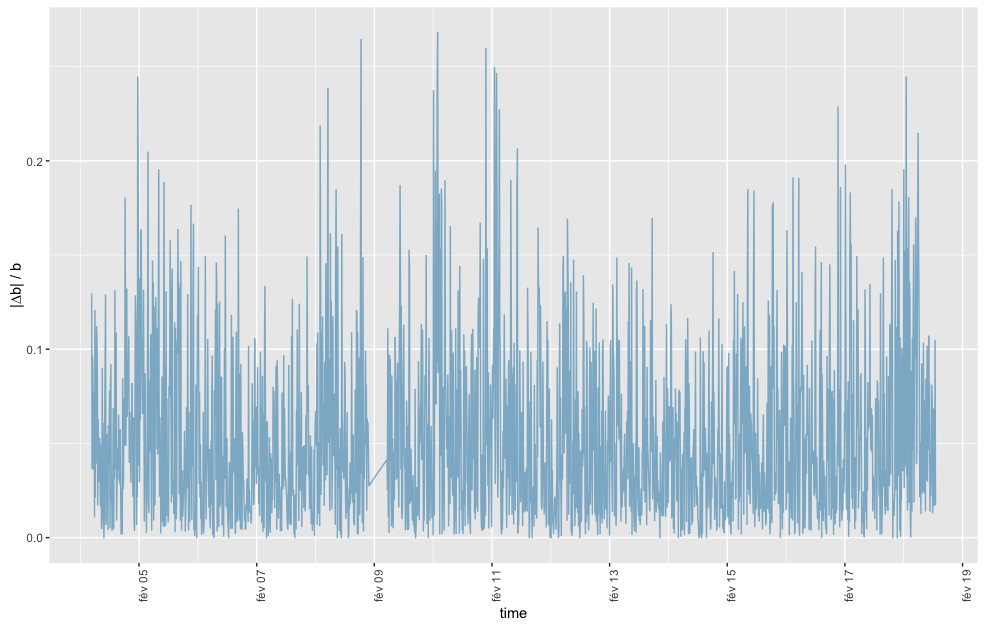
\includegraphics[width=\textwidth]{Figures/TransportationEquilibrium/gr4}
\caption{}
%\caption{\bpar{Temporal stability of maximal betweenness centrality. We plot in time the normalized derivative of maximal betweenness centrality, that expresses its relative variations at each time step. The maximal value up to 25\% correspond to very strong network disruption on the concerned link, as it means that at least this proportion of travelers assumed to take this link in previous conditions should take a totally different path.}{Stabilité temporelle du maximum de la centralité de chemin. Le graphe montre dans le temps la dérivée normalisée du maximum de la centralité de chemin, qui capture ses variations relatives à chaque pas de temps. La valeur maximale de 25\% correspond à de très fortes perturbations du réseau sur les liens correspondants, puisque cela implique qu'au moins cette proportion d'utilisateurs prenant le lien dans des conditions précédentes doivent prendre un trajet complètement différent.}}
\label{fig:fig-4}
\end{figure}
%%%%%%%%%%%%%%%%%%%





%%%%%%%%%%%%%%%%%%%
\subsection{Spatial heterogeneity of equilibrium} % Hétérogénéité spatiale de l'équilibre



\bpar{
To obtain a different insight into spatial variability of congestion patterns, we propose to use an index of spatial autocorrelation, the Moran index (defined e.g. in~\cite{tsai2005quantifying}). More generally used in spatial analysis with diverse applications from the study of urban form to the quantification of segregation, it can be applied to any spatial variable. It allows to establish neighborhood relations and unveils spatial local consistence of an equilibrium if applied on localized traffic variable. At a given point in space, local autocorrelation for variable c is computed by

%%%%%%%%%%%%
% Moran index def
\begin{equation}
\rho_i = \frac{1}{K}\cdot \sum_{i\neq j}{w_{ij}\cdot (c_i - \bar{c})(c_j - \bar{c})}
\end{equation}
%%%%%%%%%%%%

where $K$ is a normalization constant equal to the sum of spatial weights times variable variance and $\bar{c}$ is variable mean. In our case, we take spatial weights of the form $w_{ij} = \exp{\left(\frac{-d_{ij}}{d_0}\right)}$ with $d_0$ typical decay distance and compute the autocorrelation of link congestion localized at link center. We capture therefore spatial correlations within a radius of same order than decay distance around the point $i$. The mean on all points yields spatial autocorrelation index $I$. A stationarity in flows should yield some temporal stability of the index.
}{
Afin d'obtenir un point de vue différent sur la variabilité spatiale des motifs de congestion, nous proposons d'utiliser un indice d'auto-corrélation spatiale, l'indice de Moran (défini par exemple dans~\cite{tsai2005quantifying}). Utilisé plus généralement en analyse spatiale, avec diverses applications allant de l'étude de la forme urbaine à la quantification de la ségrégation, il peut être appliqué à toute variable spatiale. Il permet d'établir des relations de voisinage et révèle la consistence spatiale locale d'un équilibre s'il est appliqué à une variable de traffic localisée. A un point donnée de l'espace, l'auto-corrélation locale pour la variable $c$ est calculée par

%%%%%%%%%%%%
% Moran index def
\begin{equation}
\rho_i = \frac{1}{K}\cdot \sum_{i\neq j}{w_{ij}\cdot (c_i - \bar{c})(c_j - \bar{c})}
\end{equation}
%%%%%%%%%%%%

où $K$ est une constante de normalisation égale à la somme des poids spatiaux fois la variance de la variable et $\bar{c}$ est la moyenne de la variable. Dans notre cas, nous choisissons des poids spatiaux de la forme $w_{ij} = \exp{\left(\frac{-d_{ij}}{d_0}\right)}$ avec $d_0$ distance typique de décroissance. L'auto-corrélation est calculée sur la congestion des liens, localisée au centre du lien. Elle capture ainsi les corrélations spatiales dans un rayon du même ordre que la distance de décroissance autour du point $i$. La moyenne sur l'ensemble des points fournit l'indice d'auto-corrélation spatiale $I$. Une stationnarité des flots devrait impliquer une stabilité temporelle de l'index. 
}



\bpar{
Figure~\ref{fig:fig-5} presents temporal evolution of spatial autocorrelation for congestion. As expected, we have a strong decrease of autocorrelation with distance decay parameter, for both amplitude and temporal average. The high temporal variability implies short time scales for potential stationarity windows. When comparing with congestion (fitted to plot scale for readability) for 1km decay, we observe that high correlations coincide with off-peak hours, whereas peaks involve vanishing correlations. Our interpretation, combined with the observed variability of spatial patterns, is that peak hours correspond to chaotic behaviour of the system, as jams can emerge in any link: correlation thus vanishes as feasible phase space for a chaotic dynamical system is filled by trajectories in an uniform way what is equivalent to apparently independent random relative speeds.
}{
La figure~\ref{fig:fig-5} présente l'évolution temporelle de l'auto-corrélation spatiale pour la congestion. Comme attendu, on observe une forte décroissance de l'auto-corrélation avec la distance de décroissance, à la fois sur l'amplitude et les moyennes temporelles. La forte variabilité temporelle implique de courtes échelles temporelles pour des fenêtres potentielles de stationnarité. Pour une distance de décroissance de 1km, en comparant l'auto-corrélation à la congestion (ajustée à l'échelle du graphe pour lisibilité), on observe que les fortes corrélations coincident avec les heures creuses, tandis que les heures de pointe correspondent à une décroissance des corrélations. Notre interprétation, combinée avec la variabilité observée des motifs spatiaux, est que les heures de pointe correspondent à un comportement chaotique du système, puisque les bouchons peuvent émerger dans n'importe quel lien du réseau : la corrélation disparait alors puisque l'espace des phases atteignables pour un système dynamique chaotique est rempli uniformément par les trajectoires, de façon équivalente à des vitesses relatives qui apparaitraient comme aléatoires et indépendantes.
}



%%%%%%%%%%%%%%%%
\begin{figure}
% Spatial 
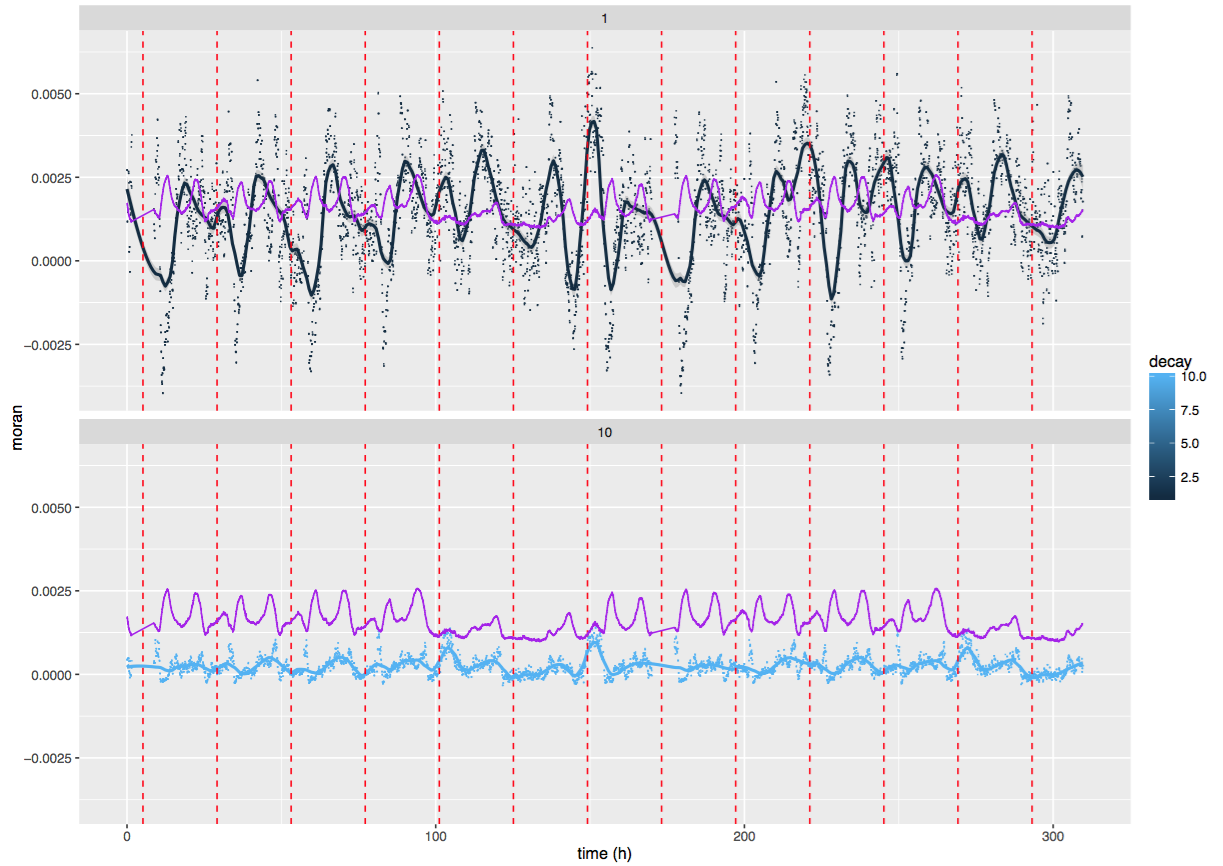
\includegraphics[width=\textwidth,height=0.6\textheight]{Figures/TransportationEquilibrium/gr5}
\caption{}
%\caption{\bpar{Spatial auto-correlations for relative travel speed on two weeks. We plot for varying value of decay parameter (1,10km) values of auto-correlation index in time. Intermediate values of decay parameter yield a rather continuous deformation between the two curves. Points are smoothed with a 2h span to ease reading. Vertical dotted lines correspond to midnight each day. Purple curve is relative speed fitted at scale to have a correspondence between auto-correlation variations and peak hours.}{Auto-corrélations spatiales pour les vitesses relatives sur deux semaines. Le graphe montre les valeurs de l'auto-corrélation dans le temps, pour des valeurs variables (1,10km) de la distance de décroissance. les valeurs intermédiaires de la distance de décroissance donnent une déformation relativement continue entre ces deux extrêmes. Les points sont lissés sur une fenêtre temporelle de 2h pour faciliter la lecture. Les lignes pointillées verticales correspondent à minuit de chaque jour. La courbe violette donne la vitesse relative, ajustée à l'échelle pour établir la correspondance entre les heures de pointe et les variations de l'auto-corrélation.}}
\label{fig:fig-5}
\end{figure}
%%%%%%%%%%%%%%%%




%%%%%%%%%%%%%%%%%%%%
\section{Discussion}

\subsection{Theoretical and practical implications of empirical conclusions}

\bpar{
We argue that the theoretical implications of our empirical findings do not imply in a total discarding of the Static User Equilibrium framework, but unveil more a need of stronger connections between theoretical literature and empirical studies. If each newly introduced theoretical framework is generally tested on one on more case study, there are no systematic comparisons of each on large and different datasets and on various objectives (prediction of traffic, reproduction of stylized facts, etc.) as systematic reviews are the rule in therapeutic evaluation for example. This imply however broader data and model sharing practices than the current ones. The precise knowledge of application potentialities for a given framework may induce unexpected developments such as its integration into larger models. The example of Land-use and Transportation Interaction studies (LUTI models) is a good illustration of how the SUE can still be used for larger purpose than transportation modeling. \cite{kryvobokov2013comparison} describe two LUTI models, one of which includes two equilibria for four-step transportation model and for land-use evolution (households and firms relocation), the other being more dynamical. The conclusion is that each model has its own advantages regarding the pursued objective, and that the static model can be used for long time policy purposes, whereas the dynamic model provide more precise information at smaller time scale. In the first case, a more complicated transportation module would have been complicated to include, what is an advantage of the static user equilibrium.
}{
Nous prétendons que les implications théoriques de ces résultats empiriques n'impliquent pas nécessairement un rejet total du cadre de l'Equilibre Utilisateur Statique, mais révèlent plutôt un besoin de plus fortes connexions entre la littérature théorique et les études empiriques. Si chaque nouveau cadre théorique introduit est généralement testé sur un cas ou plus, il n'existe pas de comparaisons systématiques de chacun sur des jeux de données de grande taille et variés, et pour des objectifs d'application différents (prédiction du traffic, reproduction de faits stylisés, etc.), à l'image des revues systématiques qui sont la règle en évaluation thérapeutique par exemple. Cela implique cependant des pratiques de partage des données et des modèles plus larges que celles existant couramment. La connaissance précise des potentialités d'application d'un cadre donné peut induire des développements inattendus comme l'intégration dans des modèles plus larges. L'exemple des études des interaction entre Transport et Usage du Sol (modèles \emph{LUTI}) est une bonne illustration d'un cas ou le EUS peut toujours être utilisé avec des motivations plus larges que la modélisation du traffic. \cite{kryvobokov2013comparison} décrit deux modèles \emph{LUTI}, dont l'un inclut deux équilibres pour les modèles de transport à quatre temps et pour l'évolution de l'usage du sol (localisation des ménages et emplois), l'autre étant dynamique. La conclusion est que chaque modèle à ses avantages au regard de l'objectif poursuivi, et que le modèle statique peut être utilisé pour comparer des politiques sur le temps long, tandis que le modèle dynamique fournit de l'information plus précise à de plus petites échelles temporelles. Dans le premier cas, un module de transport plus compliqué aurait été plus difficile à inclure, ce qui est un avantage du EUS dans ce cas.
}


\bpar{
Concerning practical applications, it seems natural that static models should not be used for traffic forecast and management at small time scales (week or day) and efforts should be made to implement more realistic models. However the use of models by the planning and engineering community is not necessarily directly related to academic concerns and state-of-the-art. For the particular case of France and mobility models, \cite{commenges2013invention} showed that engineers had gone to the point of constructing inexistent problems and implementing corresponding models that they had imported from a totally different geographical context (planning in the United States). The use of one framework or type of model has historical reasons that may be difficult to overcome.
}{
Concernant les applications pratiques, il semble naturel que les modèles statiques ne devraient pas être utilisés pour la prédiction et la gestion du traffic sur de petites échelles temporelles (semaine ou jour) et que des efforts doivent être faits pour implémenter des modèles plus réalistes. Cependant, l'utilisation des modèles par la communautés des ingénieurs et des planificateurs n'est pas directement reliée aux enjeux académiques et à l'état de l'art dans le domaine. Dans le cas particulier de la France et des modèles de mobilité, \cite{commenges2013invention} a montré que les ingénieurs allaient jusqu'au point de construire des problèmes inexistants et d'implémenter les modèles correspondants qu'ils avaient importé d'un contexte géographique totalement différent (la planification aux Etats-Unis). L'utilisation d'un cadre ou d'un type de modèle a des raisons historiques qui peuvent être difficiles à surmonter.

}


\subsection{Towards explanative interpretations of non-stationarity}


\bpar{
An assumption we formulate regarding the origin of non-stationarity of network flows, in view of data exploration and quantitative analysis of the database, is that the network is at least half of the time highly congested and in a critical state. The off-peak hours are the larger potential time windows of spatial and temporal stationarity, but consist in less than half of the time. As already interpreted through the behavior of autocorrelation indicator, a chaotic behavior may be at the origin of such variability in the congested hours. The same way a supercritical fluid may condense under the smallest external perturbation, the state of the link may qualitatively change with a small incident, producing a network disruption that may propagate and even amplify. The direct effect of traffic events (notified incidents or accidents) can not be studied without external data, and it could be interesting to enrich the database in that direction. It would allow establishing the proportion of disruptions that do appear to have a direct effect and quantify a level of criticality of network congestion in time, or to investigate more precise effects such as the consequences of an incident on traffic of the opposite lane.
}{
Une hypothèse qu'on peut formuler concernant l'origine de la non-stationnarité des flots dans le réseau, au regard de l'exploration des données et des analyses quantitatives, est que le réseau est au moins la moitié du temps fortement congestionné et dans un état critique. Les heures creuses sont les plus grandes fenêtres temporelles potentielles de stationnarité spatiale et temporelle, mais couvre moins de la moitié du temps. Comme déjà interprété dans le comportement de l'indicateur d'auto-corrélation, un comportement chaotique pourrait être à l'origine d'une telle variabilité lors des heures congestionnées. A la manière d'un fluide supercritique qui condense sous une perturbation externe infinitésimale, l'état d'un lien peut qualitativement changer par un petit incident, produisant une perturbation du réseau qui se propage et peut même s'amplifier. L'effet direct des évènements du traffic (incidents signalés ou accidents) ne peut pas être étudié sans source de données extérieure, et un enrichissement de la base de données dans cette direction pourrait être intéressante. Cela permettrait d'établir la proportion de perturbations qui paraissent avoir un effet direct et quantifier un niveau de caractère critique de la congestion du réseau dans le temps, ou d'étudier plus précisément des phénomènes localisés comme les conséquences d'un incident de traffic sur la voie opposée.
}



\subsection{Possible developments}


\bpar{
Further work may be planned towards a more refined assessment of temporal stability on a region of the network, i.e. the quantitative investigation of consideration of peak stationarity given above. To do so we propose to compute numerically Liapounov stability of the dynamical system ruling traffic flows using numerical algorithms such as described by~\cite{goldhirsch1987stability}. The value of Liapounov exponents provides the time scale by which the unstable system runs out of equilibrium. Its comparison with peak duration and average travel time, across different spatial regions and scales should provide more information on the possible validity of the local stationarity assumption. This technique has already been introduced at an other scale in transportation studies, as e.g.~\cite{tordeux2016jam} that study the stability of speed regulation models at the microscopic scale to avoid traffic jams.
}{
Le travail futur pourra être planifié dans la direction d'une étude raffinée de la stabilité temporelle sur des zones du réseau, i.e. l'étude quantitative précise de la non-stationnarité des heures de pointes découverte ci-dessus. Pour cela nous proposons de calculer numériquement la stabilité de Liapounov du système dynamique régissant les flots de traffic, par l'intermédiaire d'algorithmes numériques comme ceux décrits par~\cite{goldhirsch1987stability}. La valeur des exposants de Liapounov fournit l'échelle de temps sur laquelle le système instable s'éloigne de l'équilibre. Leur comparaison avec la durée des heures de pointe et le temps de trajet moyen, sur différentes zones spatiales et différentes échelles, devrait fournir plus d'information sur une possible validité de l'hypothèse de stationnarité locale. Cette technique a déjà été introduite à une autre échelle dans les études de transport, comme e.g.~\cite{tordeux2016jam} qui étudie la stabilité des modèles de régulation de vitesse à l'échelle microscopique pour éviter l'émergence de congestion.
}


\bpar{
Other research directions may consist in the test of other assumptions of static user equilibrium (as the rational shortest path choice, which would be however difficult to test on such an aggregated dataset, implying the use of simulation models calibrated and cross-validated on the dataset to compare assumptions, without necessarily a direct clear validation or invalidation of the assumption), or the empirical computation of parameters in stochastic or dynamical user equilibrium frameworks. 
}{
D'autres directions de recherche peuvent consister en le test des autres hypothèses du EUS (comme le choix rationnel du plus court chemin, qui serait cependant difficile à tester à un tel niveau d'agrégation, impliquant l'utilisation de modèles de simulation calibrés et cross-validés sur le jeu de données pour comparer différentes hypothèses, sans toutefois nécessairement une validation ou invalidation directe de l'hypothèse), ou le calcul empirique des paramètres dans les cadres d'Equilibre Utilisateur Stochastique ou Dynamique.
}


\section{Conclusion}


\bpar{
We have described an empirical study aimed at a simple but from our point of view necessary investigation of the existence of the static user equilibrium, more precisely of its stationarity in space and time on a metropolitan highway network. We constructed by data collection a traffic congestion dataset for the highway network of Greater Paris on 3 months with two minutes temporal granularity. The interactive exploration of the dataset with a web application allowing spatio-temporal data visualization helped to guide quantitative studies. Spatio-temporal variability of shortest paths and of network topology, in particular betweenness centrality, revealed that stationarity assumptions do not hold in general, what was confirmed by the study of spatial autocorrelation of network congestion. We suggest that our findings highlight a general need of higher connections between theoretical and empirical studies, as our work can discard misunderstandings on the theoretical static user equilibrium framework and guide the choice of potential applications.
}{
Nous avons décrit une étude empirique ayant pour but une étude simple, mais selon notre point de vue nécéssaire, de l'existence de l'équilibre utilisateur statique, plus précisément de sa stationnarité dans le temps et l'espace pour un réseau routier métropolitain principal. Un jeu de données de congestion du trafic est construite par collection de données, pour le réseau du Grand Paris sur 3 mois avec une granularité temporelle de 2 minutes. L'exploration interactive du jeu de données via une application web permettant la visualisation spatio-temporelle aide à guider les analyses quantitatives. La variabilité spatio-temporelle des plus courts chemins et de la topologie du réseau, en particulier la centralité de chemin, révèle que l'hypothèse de stationnarité ne tient généralement pas, ce qui est confirmé par l'étude de l'auto-corrélation spatiale de la congestion du réseau. Nous suggérons que nos résultats soulignent un besoin général de plus grandes connexions entre les études théoriques et empiriques, puisque cette étude permet de chasser les incompréhensions théoriques sur l'Equilibre Utilisateur Statique, et guider le choix d'application potentielles.
}










%%%%%%%%%%%%%%%
% Stylized facts : empirical analysis



% Chapter 

\chapter{Empirical Analysis : Insights from Stylized Facts} % Chapter title

\label{ch:empirical} % For referencing the chapter elsewhere, use \autoref{ch:name} 

%----------------------------------------------------------------------------------------


\headercit{Mais ce n'est pas une question d'{\^a}ge, de chiffres et de stats\\ Moi je te parle surtout de rage, de kif et d'espoir}{Youssoupha}{\textit{, Esperance de Vie}}





%  plan : 

%  1) static morphological analysis : requires a formal link between temporal and spatial correlations ?  -- typology etc can already be interesting --


%  2) presentation of BP case study

%  3) base Bien

%  4) Work with Solène



%----------------------------------------------------------------------------------------


As this quote suggests, a purely quantitative view of the world makes no sense without qualitative counterbalancing. More precisely, we argue that the \textit{clich{\'e}} of an opposition between quantitative and qualitative analysis is an illusion. No distinct boundary exists between both. We propose to call quantitative any process involving computation by a Turing machine, whereas the qualitative will be for us the modeling design process and its interpretations. Therefore both are necessarily closely interlaced in any of our approaches. In particular concerning the construction and the validation or refutation of our theory, empirical analysis on real case studies, implying the extraction and qualification of stylized facts, follows that schema.


We propose in this chapter various empirical analysis on different objects at different scales.
% articulation with theoretical questions
% articulation with modeling


%----------------------------------------------------------------------------------------


%%%%%%%%
%  Section : static analysis
%%%%%%%%

\newpage

\section{Static correlations of urban form and network shape for European territorial systems}


Spatio-temporal processes implying diffusion or propagation phenomena generally have a specific structure of correlation. In particular, as derived in section~\ref{sec:spatiotempcorrs}, a static computation of correlation between different instances of a system may under certain conditions provide information on dynamical correlations implied.


% justify scale studied here


%%%%%%%%%%%%%%%%%%
\subsection{Morphological Measures of European Population Density}

\subsubsection{Context}

At the macroscopic scale of system of cities, spatialization of the urban system is reasonably captured by cities position, associated with aggregated city variable to represent entirely the system (see e.g. ontologies of Simpop models~\cite{pumain2012multi} or its successor Marius~\cite{cottineau2014evolution}). At the mesoscopic scale at which we aim to capture morphological manifestations of interactions between transportation networks and territories, structure of the territorial system can be specified by more refined indicators for the morphological aspect. 
% biblio spatial structure etc Florent

\subsubsection{Empirical Analysis}

We study systematically morphological indicators for constant size areas covering European Community. The choice of fixed size areas can be questioned regarding definition of a territorial system, that can be otherwise understood as a consistent spatial entity at a given scale and along certain criteria : \emph{Human territories} as defined by Raffestin (op. cit.) or more generally functionally autonomous spaces\footnote{for example, a tentative of definition of a \textit{Parisian} territory would present many facets. From the subjective territory point of view, intra-muros Parisians consider a strict boundary at \textit{Boulevard Periph{\'e}rique}, whereas close and even further suburbs will be seen as Parisians from the Province. The functional territory of \textit{Metropolitain} extends slightly further than the administrative boundary. Governance perimeters are currently mutating with the Metropolitan governance project. Complementary perceptions of the territory can thus be multiplied.}.




%%%%%%%%%%%%%%%%%%
\subsection{Network Measures}

We consider network aggregated indicators as a way to characterize transportation network properties on a given territory, the same way morphological indicators yielded information on urban structure. We propose to compute some simple indicators on same extents as for morphology, to be able to explore relations between these static measures.

\subsubsection{Data preprocessing}

We work in a first time on road network, which structure is finely conditioned to territorial configuration of population densities. Furthermore, data for present day road network is available through the OpenStreetMap project~\cite{openstreetmap}. Its quality was investigated for different countries such as England~\cite{haklay2010good} and France~\cite{girres2010quality}. It was found to be of a quality equivalent to official surveys for the primary road network.

% data collected from http://download.geofabrik.de/europe.html


\paragraph{Simplification algorithm}

For a given dataset corresponding to a subset of the overall road network, it is necessary to simplify network structure by spatial aggregation as initial data presents very detailed features and thus a very large numbers of nodes ($\simeq 10^10$ for Europe dataset). Such a level of precision is not needed in our study since density data is already aggregated at 500m resolution. It is possible to drastically reduce network size by spatial aggregation of nodes and link replacements. More precisely we use the following procedure :
\begin{itemize}
\item a background raster (which resolution $r$ gives the snapping parameter for aggregation) is constructed from a reference raster and the extent of network. This grid gives spatial aggregation units for network nodes.
\item for each feature of the road dataset, corresponding connected raster cells are stored with corresponding impedance and distance in a sparse adjacency matrix.
\end{itemize}


\paragraph{Implementation}

A \texttt{PostGIS} database is used to store raw and simplified network, in order to perform efficient spatial requests, compared for example to initial \texttt{osm} data formats (\texttt{osm} or \texttt{pbf}). However


\paragraph{Sensitivity to simplification parameters}

% -> sensitivity to \theta_snap
% -> sensitivity to degree simplification (influence on means e.g.)


\subsubsection{Indicators}

Network macroscopic structure is summarized by the following set of indicators, after the simplifications and reductions done in the previous step. Assuming network given by $N=(V,E)$, nodes spatial positions $\vec{x}(V)$ and edges \emph{effective distances} $d(E)$ taking into account impedances and real distances (to include basically network hierarchy), we have indicators :
\begin{itemize}
\item connectivity
\item degree distribution
\item centrality, taken as normalized mean \emph{betweenness-centrality}
\item average path length
\item network diameter
\item mean network speed
\end{itemize}

These indicators are used to capture a rough picture of the structure. Refined work at smaller scales (intra-urban road network) and with more elaborated measures that allow to differentiate more precisely local form, was recently done by Lagesse in~\cite{2015arXiv151201268L}.



\subsubsection{Results}




%%%%%%%%%%%%%%%%%%
\subsection{Effective static correlations}



%%%%%%%%%%%%%%%%%%
\subsection{Insights for interaction processes}






%----------------------------------------------------------------------------------------


\newpage

\section{Disentangling co-evolutions from causal relations : a case study on \emph{Bassin Parisien}}




\subsection{Context Formalization}

\subsubsection{Variables}

\paragraph{Description}

We assume a dynamic transportation network $n(\vec{x},t)$ within a dynamic territorial landscape $\vec{T}(\vec{x},t)$, which components are to simplify population $p(\vec{x},t)$ and employments $e(\vec{x},t)$. Data is structured the following way :
\begin{itemize}
\item Observation of territorial variables are discretized in space and in time, i.e. the spatial field $\vec{T}$ is summarized by $\mathbf{T} = \left(\vec{T}(\vec{x}_i,t_j^{(T)})\right)_{i,j}$ with $1\leq i \leq N$ and $1\leq j \leq T$. They concretely correspond to census on administrative units (\emph{communes} in our case) at different dates.
\item Network has a continuous spatial position but
\end{itemize}



\paragraph{Definitions}



\subsection{On Accessibility}

% accessibility : need to introduce it ?
%  -> read Weibull

The notion of accessibility has been central to regional science since its introduction and systematization in planning around 1970. 

\paragraph{Existence of accessibility}

%An elegant axiomatic definition is derived in~\cite{weibull1976axiomatic}. Starting from expected properties of an accessibility function $A$ that associate a value to \emph{attraction} $a$ and distance $d$, defined on the set of discrete spatial configurations $\mathcal{C} = \cup_{n\in \mathbb{N}}{(d_i,a_i)_{1\leq i \leq n}}$. These properties include (among technical others with no thematic meaning) :
%\begin{enumerate}
%\item $A$ is invariant regarding the order of the configuration
%\item $A$ decrease with distance at fixed attraction and increase with attraction at fixed distance
%\item $A$ is invariant when adding null attractions and constant configurations
%\end{enumerate}

%A canonical decomposition of any accessibility function 




\textit{\textbf{Is the notion of accessibility crucial for statistical analysis ?}}

\medskip


Weibull has proposed an axiomatic approach to accessibility~\cite{weibull1976axiomatic}, deriving a canonical decomposition for any \emph{attraction-accessibility} function $A(a,d)$, assuming expected thematic axioms among others technical ones that are :
\begin{enumerate}
\item \footnotesize $A$ is invariant regarding the order of the configuration
\item \footnotesize $A$ decrease with distance at fixed attraction and increase with attraction at fixed distance
\item \footnotesize $A$ is invariant when adding null attractions and constant configurations
\end{enumerate}
Then $A$ verifies these \emph{iff} it is of the form
\[
A\left[(a_i,d_i)\right] = T\left(\bigoplus_i z(d_i,a_i)\right)
\]
where $T$ is increasing with null origin, $z$ is a \emph{distance substitution function} (i.e. verifying axiom 2) and $\oplus$ a \emph{standard composition} associating two attractions at zero distance to th corresponding unique one. 

$\rightarrow$ \textit{Well suited matrices of autocorrelation should capture accessibility in regressions ; or captured by non-linear regression on $\mathbf{N}$}

\medskip

{\normalsize\textit{\textbf{Accessibility as potential ?}}}

Given any stationary dynamic for $n,\vec{T}$, Helmoltz theorem states that it derives from a potential (can be adapted to non-stationary dynamics with time-varying potential).








\paragraph{Continuous approach and accessibility potential}

% Paul : Helmoltz-Hodge theorem to infer potential field from speed spatial field ?
%  Q : what are trajectories ? dirac field has no rotational -> continuous approach does not work ?






\subsection{Statistical Tests}



\textit{Large set of analysis to be tested (non exhaustive) :}
\begin{itemize}
\item On data :
\begin{itemize}
\item Multivariate models $\mathcal{L}\left[\mathbf{T},\mathbf{N}\right]\sim \varepsilon$
\item Autocorrelated univariate models $(\mathbf{I} - \Sigma R W) \mathbf{X} \sim \varepsilon$
\item Autocorrelated multivariate models $(\mathcal{L}' - \Sigma R W)\left[\mathbf{T}+\mathbf{N}\right] \sim \varepsilon$
\item Geographically Weighted Regression~\cite{brunsdon1998geographically}
\[
\mathcal{L}\left[\mathcal{G}\left(\mathbf{T},\mathbf{N}\right)\right] \sim \varepsilon
\]
\item Granger causality tests : \cite{xie2009streetcars} use Granger causality to link transit with land-use changes.
\end{itemize}
\item On data returns :
\begin{itemize}
\item Autoregressive multivariate models
\[\mathcal{L}\left[(\Delta \mathbf{T}(t_{j'}))_{j'\leq j},(\Delta \mathbf{N}(t_{j'}))_{j'\leq j}\right] \sim \varepsilon\]
\item Autoregressive autocorrelated multivariate models : idem with spatial autocorrelation term.
\item Synthetic Instrumental Variables : static territory and/or network ?
\end{itemize}
\end{itemize}



\subsubsection{Bivariate linear models}

\subsubsection{Autocorrelated univariate models}

\subsubsection{Autocorrelated multivariate models}

\subsubsection{Granger causality tests}

\cite{xie2009streetcars} use Granger causality to link transit with land-use changes.


\subsubsection{Autoregressive multivariate models}



\subsubsection{Autoregressive autocorrelated multivariate models}











%----------------------------------------------------------------------------------------

\newpage

\section{Early warnings of Network Breakdowns : socio-economic and real estate trajectories}


\subsection{Context}

Various aspects of territories are concerned by interactions with networks. In previous empirical studies, no socio-economic attributes of populations inhabiting the territory nor economic values for land and real estate was considered. Both are however crucial elements of territorial dynamics and are extensively studied in fields such as territorial analysis or urban economics : for example, \cite{homocianu:tel-00359302} studies households residential choices to understand land-use transportation interactions.



\subsection{Preliminary Results}




\subsection{A strategy to investigate early warnings of network breakdowns}








%----------------------------------------------------------------------------------------

\section{South-African historical events as instruments to understand network-territory relations}











%%%%%%%%%%%%%%%
% Toy modeling : density model / correlated synthetic data



% Chapter 

\chapter{Modeling} % Chapter title

\label{ch:modeling} % For referencing the chapter elsewhere, use \autoref{ch:name} 





%----------------------------------------------------------------------------------------











%----------------------------------------------------------------------------------------

\newpage


% Q : synthetic data to be mentioned here ? 
%    -> may be in Methodology
%    then needs to clarify : Plan (of course) ; diagram for plan ; and dependence tree for parts/sections

\section{A simple model of urban growth}



We propose a stochastic model of urban growth that generates spatial distributions of population densities, at an intermediate scale between economic models at the macro scale and land-use evolution models focusing on local relations. Integrating simply the two opposite key processes of aggregation (“preferential attachment”) and diffusion (urban sprawl), we show that we can capture the whole spectrum of existing urban forms in Europe. An extensive exploration and calibration of the proposed model allows determining the region of parameter space corresponding morphologically to observed european urban systems, providing an validated thematic interpretation to model parameters, and furthermore determining the effective dimension of the urban system at this scale regarding morphological objectives.




%%%%%%%%%%%%%
% 1 - Introduction
\subsection{Context}
%%%%%%%%%%%%%

% - > literature on stochastic urban growth, ABM for Urban Growth, CA Models and urban morphogenesis models. Reproducing urban growth at different scales, capturing different processes.
% ⇒ Plus réponse à cette question : pourquoi simuler la croissance urbaine (quels enjeux scientifiques et sociaux ?)

% Macro models (Gibrat and extensions) are partially spatialized (Favaro - Pumain includes distance between cities, Simpops/Marius also) whereas micro (most CA) are ‘’over-spatialized’’ (neighborhood-based).  
% -> Research Question :  What about a simple model at the meso scale, close to macro by the stylized facts (preferential attachment) but producing morphologically consistent spatial distribution of densities ?



\cite{andersson2002urban} propose a micro-based model of urban growth, with the purpose to replace non-interpretable physical mechanisms with agent mechanisms, including interactions forces and mobility choices.



%%%%%%%%%%%%%%%%%
% 2 - Materials and Methods
\subsection{Model Description}
%%%%%%%%%%%%%%



% 2.2 - The urban growth model
\subsubsection{The urban growth model}

\paragraph{Rationale}

%Preferential attchment and diffusion, extension of [Batty, 2006]. small litt. prefAtt and then Urban sprawl, opposed forces that must shape morphology of urban systems. choice of a scale at which spatial form has a sense but city system is ‘’wide enough” : 50-100km, meso-scale ?

% following Florent : \cite{fujita1996economics} oppose agglomeration and sprawl

Our model is an extension of the diffusion-limited aggregation model studied in~\cite{batty2006hierarchy}. Indeed, the tension between antagonist aggregation and sprawl mechanisms may be an important process in urban morphogenesis. \cite{fujita1996economics} opposes centrifugal forces with centripetal forces in the equilibrium view of urban spatial systems, what is easily transferable to non-equilibrium systems in the framework of self-organized complexity : a urban structure is a far-from-equilibrium system that has been driven to this point by this opposite forces.



\paragraph{Settings}

Precise formulation, description and formalization of the model. ; parameters and their possible interpretation ; def of parameter space.





% 2.3 - Indicators
\subsubsection{Indicators}

% Literature on morphological analysis, method taken from [Le Nechet 2015] to qualify/quantify urban form. Why would form be relevant at this scale ? -> thematic references on variety of urban developments, rural settlements, etc. : form translates many spatial processes at this scale. [beware question of equifiniality : model is however themtically-based for processes].

% Definition of indicators




%%%%%%%%%%%%
%  3 - Results
\subsection{Results}
%%%%%%%%%%%%


Precise description of the implementation (pub openmole exploration etc, importance of intensive computation)


% 3.1 - Generation of urban patterns
\subsubsection{Generation of urban patterns}

variety of genered forms, examples of extreme shapes.













%%%%%%%%%%%%
\begin{figure}

\caption{Example of the variety of generated urban shapes}
\end{figure}
%%%%%%%%%%%%




\subsubsection{Model Behavior}


\paragraph{Convergence - internal model validation}

convergence properties of indicators ; number of repetitions needed for consistence of results. [histograms and stats of $\sigma$ %TODO]

\paragraph{Exploration of parameter space}

Grid, then LHS explorations.





%%%%%%%%%%%%
\begin{figure}

\caption{Scatterplots of indicators distribution in an hypercube of the parameter space. We show here the influence of one parameter (diffusion rate). Red points correspond to real data.}
\end{figure}
%%%%%%%%%%%%

% Q : 3D plots as supp material ?

Figure : on 2 first PC of morpho indicators, localization of typical shapes (monocentric city, polycentric city, diffuse rural settlements, aggregated rural settlements) / comparing generated shape with a typical real one

\paragraph{Statistical analysis}

Regression indics = f(params) . TO BE DONE.
interpretation ?

% 3.3 - Model Calibration
\subsubsection{Model Calibration}

% 3.3.1 - Real Data
\paragraph{Real Data}

%% Data source (density grid), computation methodology [comparison of sampling/smoothing to avoid bord effects ?] -> reals values of morpho indics on 50kmx50km grids, on all Europe.
%% + summary stats




%Figure : Distributions of indicators values for real dataset of european densities, computed on 50kmx50km grids, with 10km offset to avoid bord effects. [TODO : add log-normal/normal fits ? ]
%  -> cf Empirical Section



\paragraph{Calibration Process}

Specific calib process : PCA that maximize the cumulated distance between generated points and reals points ; then select point cloud that overlaps real points in (PC1,PC2) plan, given a distance threshold.






Figure : Precise calibration of the model. The principal component analysis is conducted to maximize the spread of the differences between real data and model output, i.e. on the set $\{\left|R_i - M_j\right|\}$ where $R_i$ is the set of real points, $M_j$ the set of model outputs. We select then the overlapping cloud at threshold $\theta$, by taking models output closer to real point cloud than $\theta$ in the (PC1,PC2) plan.


% 3.3.3 - Calibration Results
\subsubsection{Calibration Results}

-> extraction of the exact parameter space covering all real situations.
interpretation of its shape (correlations between parameters ?) and its volume in different directions (relative importance of parameters).
[possible development : application of Calibration Profile algo to check relative influence of parameters + ad hoc linear algebra on regression of 3.2.3 to do the same]






\subsection{Discussion}


\subsubsection{Thematic interpretation of growth behavior}

interpret positions of typical shapes within param space : confirms thematic interpretation of parameters.
depending on results of 3.3.3, necessary and sufficient parameters to explain growth at this scale -> interpretation ?

\subsubsection{Integration into a multi-scale growth model}

Possible coupling on a gibrat (or favaro-pumain) at europa scale (macro) (with addition of consistence on migration constraints), where meso growth rates which werer exogeneous before, are top-down determined, and bottom-up feedback is done through local aggregation level, that influence attractivity of an area.


%%%%%
%% 4.3 - Methodological application ?
%%%%% -> maybe out of scope here ?



 -> Accurately calibrated spatialized urban growth model, can reproduce any (european) urban pattern.
 -> interpretation of parameter influence ; effective independant dimensions of the urban system at this scale.




















%----------------------------------------------------------------------------------------


\newpage


% DO NOT INSERT FINANCIAL EXAMPLE ! 

\section{Correlated generation of territorial configurations}










%%%%%%%%%%%%%%%%%%%%%%
\subsection{Application : geographical data of density and network}


%%%%%%%%%%%%%%%%%%%%%%
\subsubsection{Context}


The use of synthetic data in geography is generally directed towards the generation of synthetic populations within agent-based models (mobility, \emph{LUTI} models)~\cite{pritchard2009advances}. We can make a weak link with some Spatial Analysis techniques. The extrapolation of a continuous spatial field from a discrete spatial sample through a kernel density estimation for example can be understood as the creation of a synthetic dataset (even if it is not generally the initial view, as in Geographically Weighted Regression~\cite{brunsdon1998geographically} in which variable size kernels do not interpolate data \emph{stricto sensu} but extrapolate abstract variables representing interaction between explicit variables). In the field of modeling in quantitative geography, \emph{toy-models} or hybrid models require a consistent initial spatial configuration. A set of possible initial configurations becomes a synthetic dataset on which the model is tested. The first Simpop model~\cite{sanders1997simpop}, precursor of a large family of models later parametrized with real data, could enter that frame but was studied on an unique synthetic spatialization. Similarly underlined was the difficulty to generate an initial transportation infrastructure in the case of the SimpopNet model~\cite{schmitt2014modelisation} although it was admitted as a cornerstone of knowledge on the behavior of the model. A systematic control of spatial configuration effects on the behavior of simulation models was only recently proposed~\cite{cottineau2015revisiting}, approach that can be interpreted as a statistical control on spatial data. The aim is to be able to distinguish proper effects due to intrinsic model dynamics from particular effects due to the geographical structure of the case study. Such results are essential for the validation of conclusions obtained with modeling and simulation practices in quantitative geography.



%%%%%%%%%%%%%%%%%%%%%%
\subsubsection{Formalization}

We propose in our case to generate territorial systems summarized in a simplified way as a spatial population density $d(\vec{x})$ and a transportation network $n(\vec{x})$. Correlations we aim to control are correlations between urban morphological measures and network measures. The question of interactions between territories and networks is already well-studied~\cite{offner1996reseaux} but stays highly complex and difficult to quantify~\cite{offner1993effets}. A dynamical modeling of implied processes should shed light on these interactions (\cite{bretagnolle:tel-00459720}, p. 162-163). We develop in that frame a \emph{simple} coupling (i.e. without any feedback loop) between a density distribution model and a network morphogenesis model.



\paragraph{Density model}

We use a model $D$ similar to aggregation-diffusion models~\cite{batty2006hierarchy} to generate a discrete spatial distribution of population density. A generalization of the basic model is proposed in~\cite{raimbault2016calibration}, providing a calibration on morphological objectives (entropy, hierarchy, spatial auto-correlation, mean distance) against real values computed on the set of 50km sized grid extracted from european density grid~\cite{eurostat}. More precisely, the model proceeds iteratively the following way. An square grid of width $N$, initially empty, is represented by population $(P_i(t))_{1\leq i\leq N^2}$. At each time step, until total population reaches a fixed parameter $P_m$,
\begin{itemize}
\item total population is increased of a fixed number $N_G$ (growth rate), following a preferential attachment such that 
\[\Pb{P_i(t+1)=P_i(t)+1|P(t+1)=P(t)+1}=\frac{(P_i(t)/P(t))^{\alpha}}{\sum(P_i(t)/P(t))^{\alpha}}\]
\item a fraction $\beta$ of population is diffused to four closest neighbors is operated $n_d$ times
\end{itemize}





The two contradictory processes of urban concentration and urban sprawl are captured by the model, what allows to reproduce with a good precision a large number of existing morphologies.

%Les deux processus antagonistes de concentration et d'étalement urbain sont capturés par le modèle, ce qui permet de reproduire assez fidèlement un grand nombre de morphologies existantes.


\paragraph{Network model}


On the other hand, we are able to generate a planar transportation network by a model $N$, at a similar scale and given a density distribution. Because of the conditional nature to the density of the generation process, we will first have conditional estimators for network indicators, and secondly natural correlations between network and urban shapes should appear as processes are not independent. The nature and modularity of these correlations as a function of model parameters are still to determine by exploration of the coupled model.



The heuristic network generation procedure is the following :
\begin{enumerate}
\item A fixed number $N_c$ of centers that will be first nodes of the network si distributed given density distribution, following a similar law to the aggregation process, i.e. the probability to be distributed in a given patch is $\frac{(P_i/P)^{\alpha}}{\sum (P_i/P)^{\alpha}}$. Population is then attributed according to Voronoi areas of centers, such that a center cumulates population of patches within its extent.
\item Centers are connected deterministically by percolation between closest clusters : as soon as network is not connected, two closest connected components in the sense of minimal distance between each vertices are connected by the link realizing this distance. It yields a tree-shaped network.
\item Network is modulated by potential breaking in order to be closer from real network shapes. More precisely, a generalized gravity potential between two centers $i$ and $j$ is defined by
\[
V_{ij}(d) = \left[ (1 - k_h) + k_h \cdot \left( \frac{P_i P_j}{P^2} \right)^{\gamma} \right]\cdot \exp{\left( -\frac{d}{r_g (1 + d/d_0)} \right)}
\]
where $d$ can be euclidian distance $d_{ij}=d(i,j)$ or network distance $d_N(i,j)$, $k_h \in [0,1]$ a weight to modulate role of populations, $\gamma$ giving shape of the hierarchy across population values, $r_g$ characteristic interaction distance and $d_0$ distance shape parameter.
\item A fixed number $K\cdot N_L$ of potential new links is taken among couples having greatest euclidian distance potential ($K=5$ is fixed).
\item Among potential links, $N_L$ are effectively realized, that are the one with smallest rate $\tilde{V}_{ij} = V_{ij}(d_N)/V_{ij}(d_{ij})$. At this stage only the gap between euclidian and network distance is taken into account : $\tilde{V}_{ij}$ does indeed not depend on populations and is increasing with $d_N$ at constant $d_{ij}$.
\item Planarity of the network is forced by creation of nodes at possible intersections created by new links.
\end{enumerate}



We insist on the fact that the network generation procedure is entirely heuristic and result of thematic assumptions (connected initial network, gravity-based link creation) combined with trial-and-error during first explorations. Other model types could be used as well, such biological self-generated networks~\cite{tero2010rules}, local network growth based on geometrical constraints optimization~\cite{barthelemy2008modeling}, or a more complex percolation model than the initial one that would allow the creation of loops for example. We could thus in the frame of a modular architecture, in which the choice between different implementations of a functional brick can be seen as a meta-parameter~\cite{cottineau2015incremental}, choose network generation function adapted to a specific need (as e.g. proximity to real data, constraints on output indicators, variety if generated forms, etc. ).




%  must do a computational benchmark for various network generation models ; calibrated on real data. -> cf network generation section.

\paragraph{Parameter space}

Parameter space for the coupled model\footnote{Weak coupling allows to limit the total number of parameters as a strong coupling would involve retroaction loops and consequently associated parameters to determine their structure and intensity. In order to diminish it, an integrated model would be preferable to a strong coupling, what is slightly different in the sense where it is not possible in the integrated model to freeze one of the subsystems to obtain a model of the other subsystem that would correspond to the non-coupled model.} is constituted by density generation parameters $\vec{\alpha}_D = (P_m/N_G , \alpha,\beta , n_d)$ (we study for the sake of simplicity the rate between population and growth rate instead of both varying, i.e. the number of steps needed to generate the distribution) and network generation parameters $\vec{\alpha}_N=(N_C,k_h,\gamma , r_g , d_0)$. We denote $\vec{\alpha} = (\vec{\alpha}_D,\vec{\alpha}_N)$. 




% these notion of weak / strong coupling are not enough developed or reference-based. ---> find it in literature ? not sure exists like that. --> integarte it in theoretical paper ? or separate working paper.

\paragraph{Indicators}

Urban form and network structure are quantified by numerical indicators in order to modulate correlations between these. Morphology is defined as a vector $\vec{M}=(r,\bar{d},\varepsilon,a)$ giving spatial auto-correlation (Moran index), mean distance, entropy and hierarchy (see~\cite{le2015forme} for a precise definition of these indicators). Network measures $\vec{G} = (\bar{c},\bar{l},\bar{s},\delta)$ are with network denoted $(V,E)$
\begin{itemize}
\item Mean centrality $\bar{c}$ defined as average \emph{betweeness-centrality} (normalized in $[0,1]$) on all links.
\item Mean path length $\bar{l}$ given by $\frac{1}{d_m}\frac{2}{|V|\cdot (|V|-1)}\sum_{i<j}d_N(i,j)$ with $d_m$ normalization distance taken here as world diagonal $d_m=\sqrt{2}N$.
\item Mean network speed~\cite{banos2012towards} which corresponds to network performance compared to direct travel, defined as $\bar{s} = \frac{2}{|V|\cdot (|V|-1)}\sum_{i<j}{\frac{d_{ij}}{d_N(i,j)}}$.
\item Network diameter $\delta = \max_{ij}d_N(i,j)$.
\end{itemize}




\paragraph{Covariance and correlation}

We study the cross-correlation matrix $\Covb{\vec{M}}{\vec{G}}$ between morphology and network. We estimate it on a set of $n$ realizations at fixed parameter values $(\vec{M}\left[D(\vec{\alpha})\right],\vec{G}\left[N(\vec{\alpha})\right])_{1\leq i\leq n}$ with standard unbiased estimator. We estimate correlation with associated Pearson estimator. 



%%%%%%%%%%%%%%%%%%%%%%
\subsubsection{Implementation}


Coupling of generative models is done both at formal and operational levels. We interface therefore independent implementations. The OpenMole software~\cite{reuillon2013openmole} for intensive model exploration offers for that the ideal frame thanks to its modular language allowing to construct \emph{workflows} by task composition and interfacing with diverse experience plans and outputs. For operational reasons, density model is implemented in \texttt{scala} language as an OpenMole \texttt{plugin}, whereas network generation is implemented in agent-oriented language \texttt{NetLogo}~\cite{wilensky1999netlogo} because of its possibilities for interactive exploration and heuristic model construction. Source code is available for reproducibility on project repository\footnote{at \texttt{https://github.com/JusteRaimbault/CityNetwork/tree/master/Models/Synthetic}}.





%%%%%%%%%%%%%%
\begin{figure}

\subfloat[]{%[t]{0.35\linewidth}
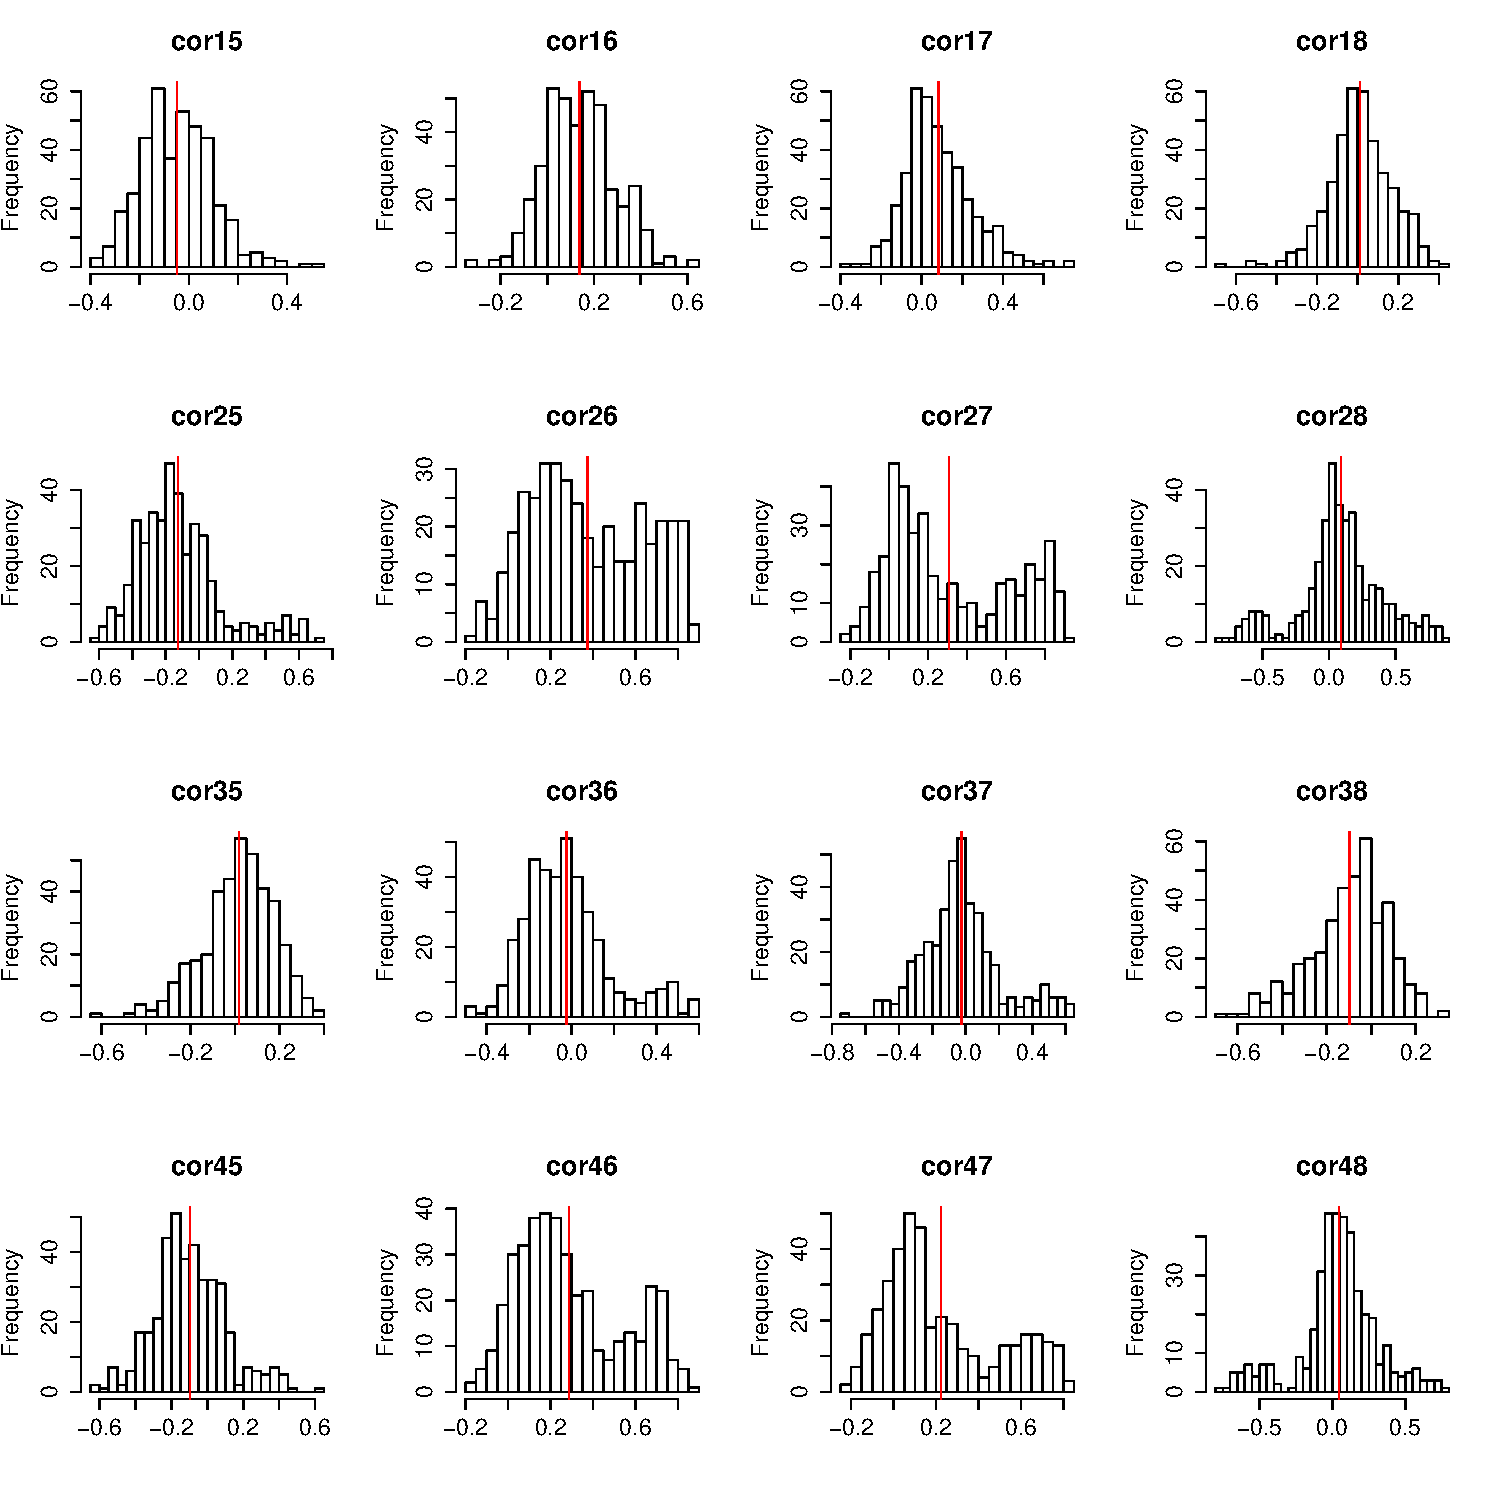
\includegraphics[width=0.35\textwidth]{Figures/PartII/Modeling/CorrelatedData/hist_crossCorMat_breaks30}
%\caption{}
}
\subfloat[]{%[t]{0.23\linewidth}
\vspace{-6.5cm}
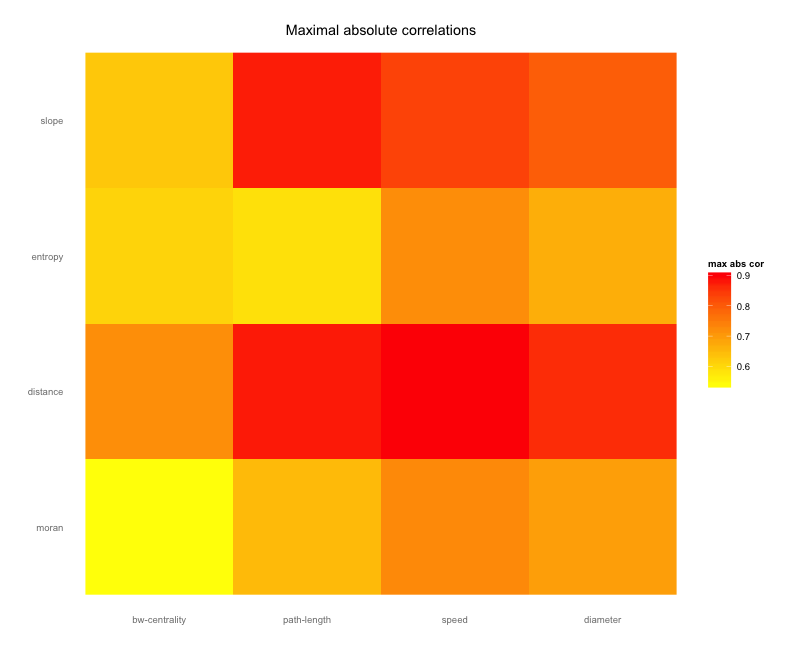
\includegraphics[width=0.23\textwidth]{Figures/PartII/Modeling/CorrelatedData/heatmap_maxAbsCor}\\
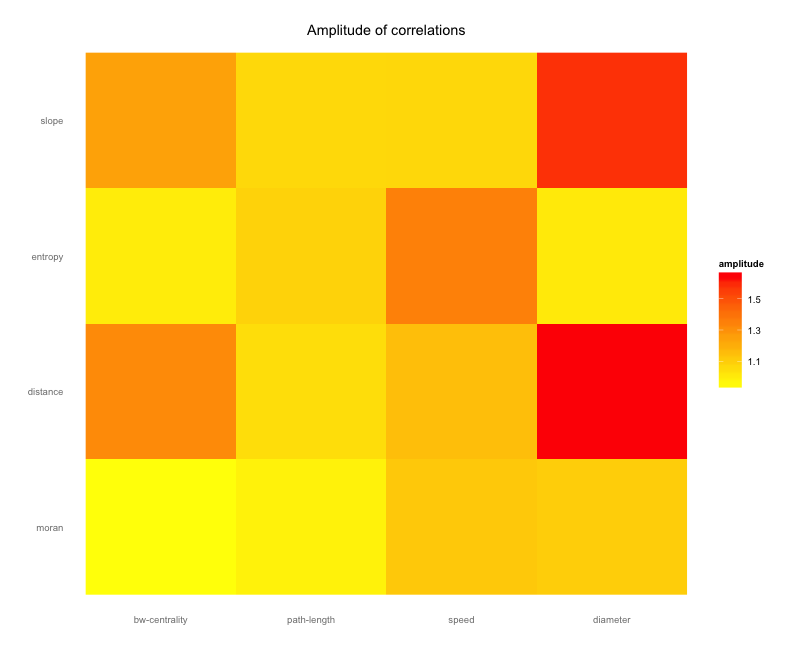
\includegraphics[width=0.23\textwidth]{Figures/PartII/Modeling/CorrelatedData/heatmap_amplCor}
}
\subfloat[]{%[t]{0.4\linewidth}
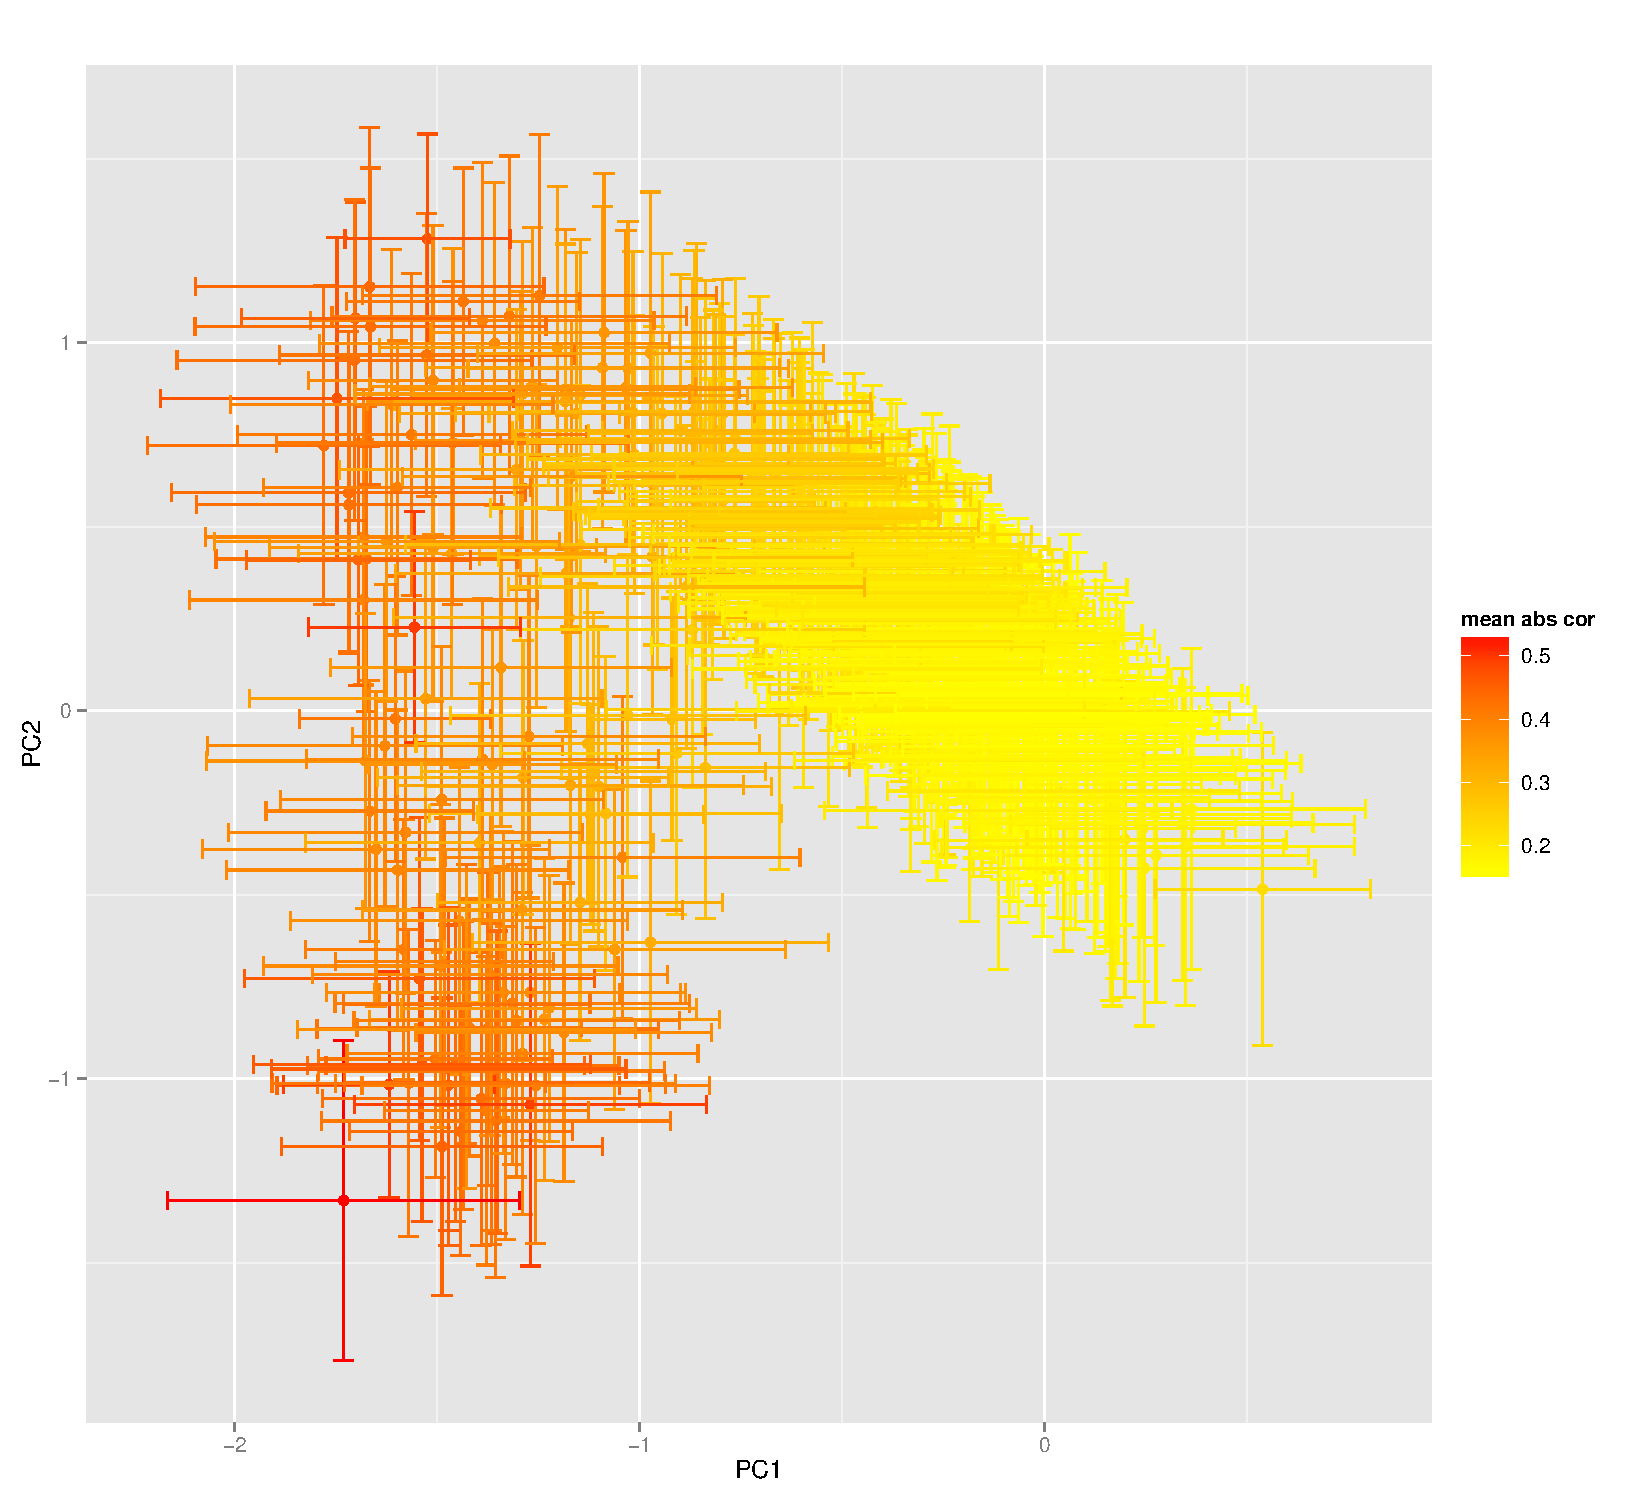
\includegraphics[width=0.4\textwidth]{Figures/PartII/Modeling/CorrelatedData/pca_meanAbsCor_errorBars}
}\\
\subfloat[]{%[t]{0.54\linewidth}
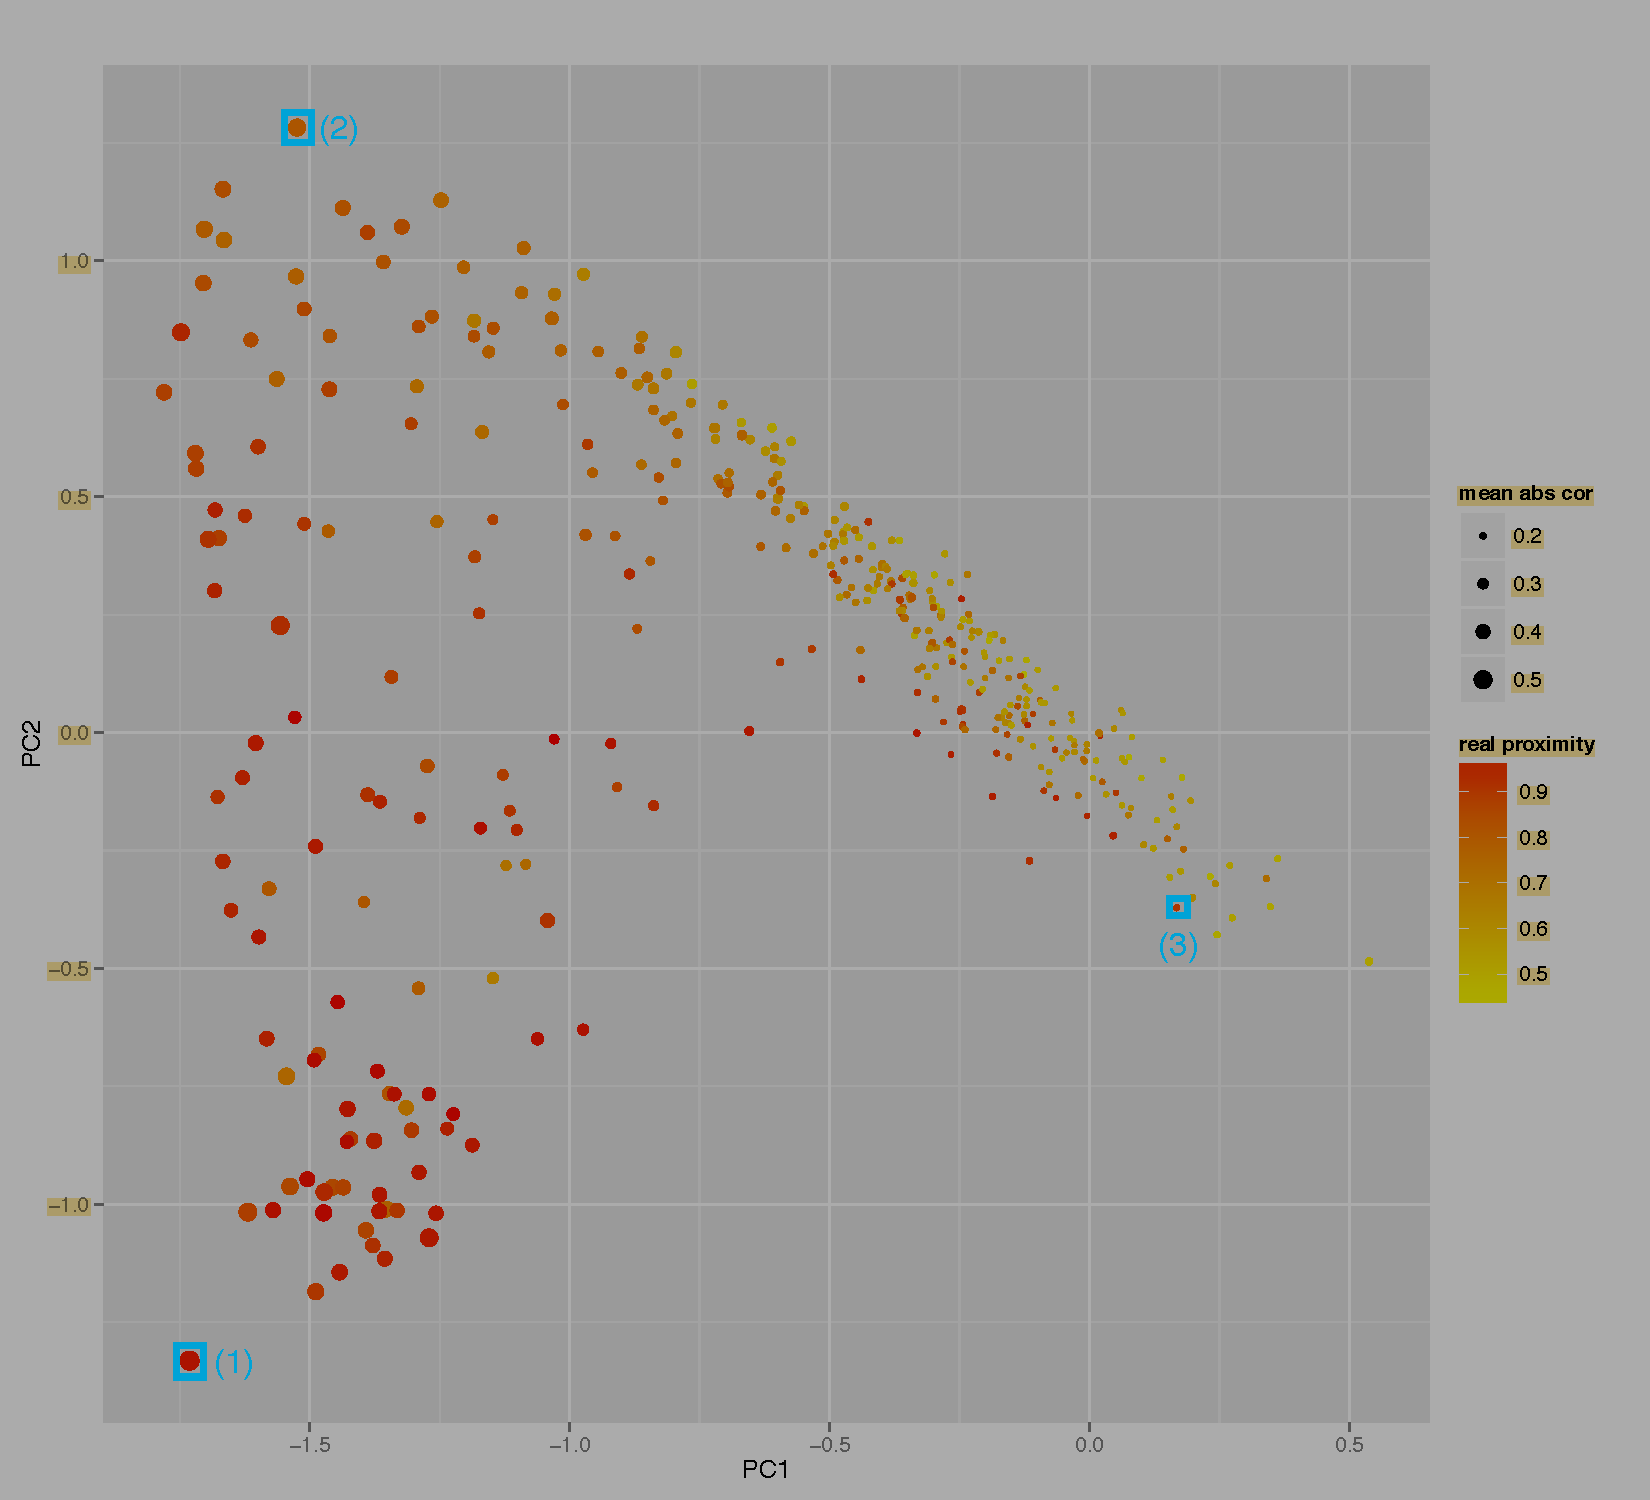
\includegraphics[width=\textwidth]{Figures/PartII/Modeling/CorrelatedData/pca_realDistCol_meanAbsCorSize_withSpecificPoints}
}
\subfloat[]{%[t]{0.45\linewidth}
\vspace{-8.3cm}
}

\caption[Exploration of feasible space for correlations between urban morphology and network structure]{\footnotesize\textbf{Exploration of feasible space for correlations between urban morphology and network structure | } \textbf{(a)} Distribution of crossed-correlations between vectors $\vec{M}$ of morphological indicators (in numbering order Moran index, mean distance, entropy, hierarchy) and $\vec{N}$ of network measures (centrality, mean path length, speed, diameter). \textbf{(b)} Heatmaps for amplitude of correlations, defined as $a_{ij}=\max_k{\rho_{ij}^{(k)}}-\min_k{\rho_{ij}^{(k)}}$ and maximal absolute correlation, defined as $c_{ij}=\max_k\left| \rho_{ij}^{k} \right|$. \textbf{(c)} Projection of correlation matrices in a principal plan obtained by Principal Component Analysis on matrix population (cumulated variances: PC1=38\%, PC2=68\%). Error bars are initially computed as 95\% confidence intervals on each matrix element (by standard Fisher asymptotic method), and upper bounds after transformation are taken in principal plan. Scale color gives mean absolute correlation on full matrices. \textbf{(d)} Representation in the principal plan, scale color giving proximity to real data defined as $1 - \min_r \norm{\vec{M}-\vec{M}_r}$ where $\vec{M}_r$ is the set of real morphological measures, point size giving mean absolute correlation.}
\label{fig:densnwcor}
\end{figure}
%%%%%%%%%%%%%%


%%%%%%%%%%%%%%
\begin{figure}
\centering

   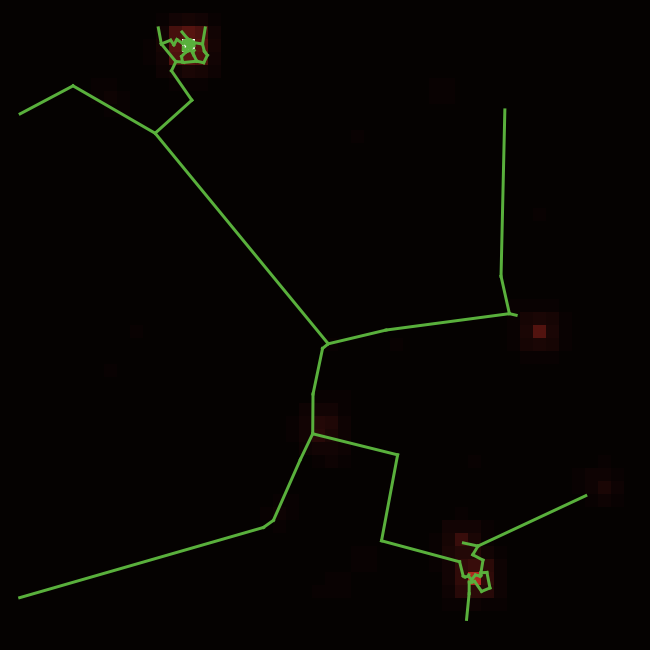
\includegraphics[width=0.5\textwidth]{Figures/PartII/Modeling/CorrelatedData/configs/1_param71861_seed0}
   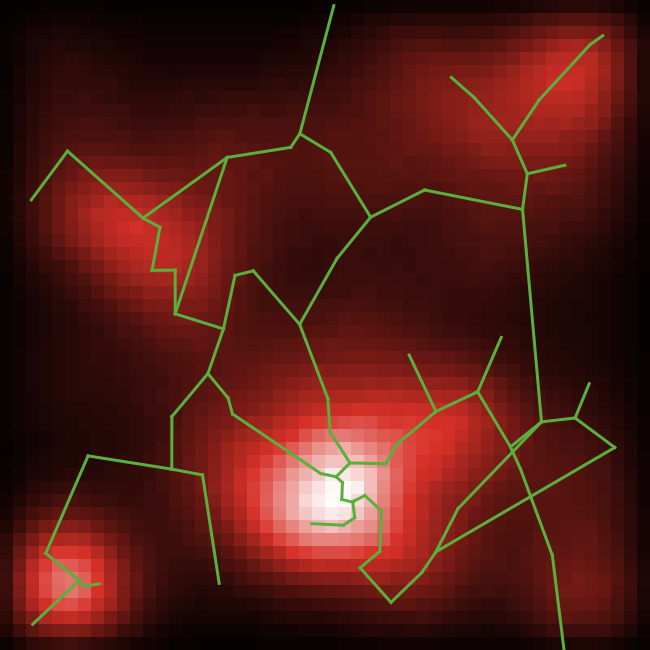
\includegraphics[width=0.5\textwidth]{Figures/PartII/Modeling/CorrelatedData/configs/2_param71913_seed10}\\
   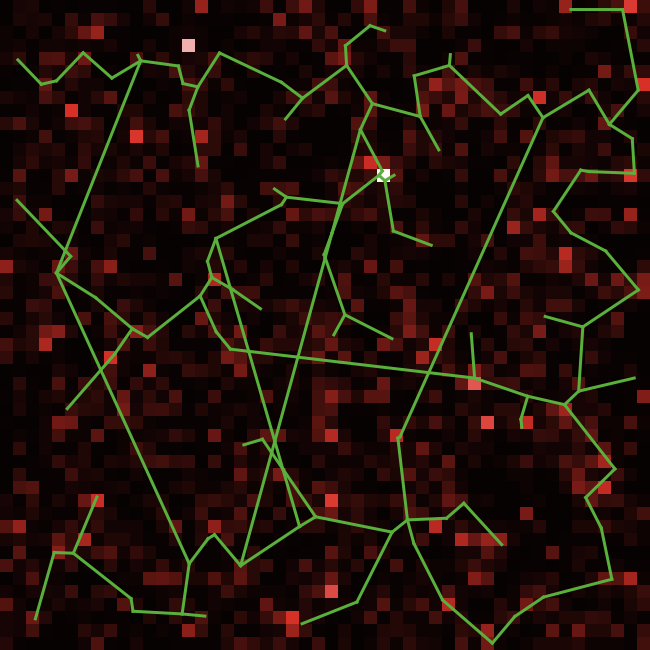
\includegraphics[width=0.5\textwidth]{Figures/PartII/Modeling/CorrelatedData/configs/3_param71918_seed0}
   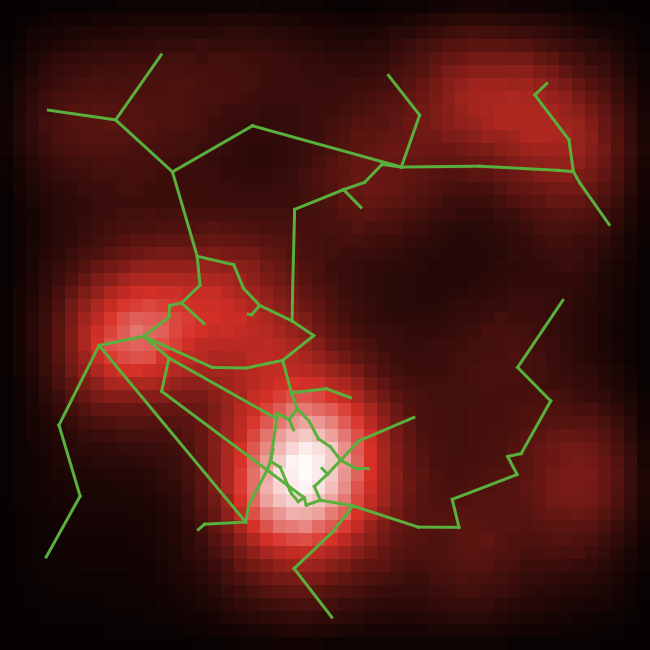
\includegraphics[width=0.5\textwidth]{Figures/PartII/Modeling/CorrelatedData/configs/4_param71945_seed0}
\caption[Examples of generated coupled configurations]{Configurations obtained for parameters giving the four emphasized points in (d), in order from left to right and top to bottom. We recognize polycentric city configurations (2 and 4), diffuse rural settlements (3) and aggregated weak density area (1). See appendice for exhaustive parameter values, indicators and corresponding correlations. For example $\bar{d}$ is highly correlated with $\bar{l},\bar{s}$ ($\simeq$0.8) in (1) but not for (3) although both correspond to rural environments ; in the urban case we observe also a broad variability : $\rho[\bar{d},\bar{c}]\simeq 0.34$ for (4) but $\simeq-0.41$ for (2), what is explained by a stronger role of gravitation hierarchy in (2) $\gamma=3.9,k_h=0.7$ (for (4), $\gamma=1.07,k_h=0.25$), whereas density parameters are similar.}
\end{figure}
%%%%%%%%%%%%%%





%%%%%%%%%%%%%%%%%%%%%%
\subsubsection{Results}

The study of density model alone is developed in~\cite{raimbault2016calibration}. It is in particular calibrated on European density grid data, on 50km width square areas with 500m resolution for which real indicator values have been computed on whole Europe. Furthermore, a grid exploration of model behavior yields feasible output space in reasonable parameters bounds (roughly $\alpha \in [0.5,2],N_G\in [500,3000], P_m \in [10^4,10^5],\beta\in [0,0.2], n_d \in \{ 1, \ldots , 4\}$). The reduction of indicators space to a two dimensional plan through a Principal Component Analysis (variance explained with two components $\simeq 80\%$) allows to isolate a set of output points that covers reasonably precisely real point cloud. It confirms the ability of the model to reproduce morphologically the set of real configurations.



% NOT NEEDED - TOO MUCH INFORMATION - ?
%%%%%%%%%%%%%%%%
%\begin{figure}
% figure : density example, exploration and calibration ?
%\end{figure}
%%%%%%%%%%%%%%%%

At given density, the conditional exploration of network generation model parameter space suggest a good flexibility on global indicators $\vec{G}$, together with good convergence properties. For a precise study of model behavior, see appendice giving regressions analysis capturing the behavior of coupled model. In order to illustrate synthetic data generation method, the exploration has been oriented towards the study of cross-correlations.


%A densité donnée, l'exploration de l'espace des paramètres du modèle de réseau suggèrent une assez bonne flexibilité sur des indicateurs globaux $\vec{G}$, ainsi que de bonnes propriétés de convergence. Pour une étude du comportement précis, voir l'appendice donnant les regressions traduisant le comportement du modèle couplé. Dans le but d'illustrer la méthode de génération de données synthétiques, l'exploration a été orientée vers l'étude des correlations.


Given the large relative dimension of parameter space, an exhaustive grid exploration is not possible. We use a Latin Hypercube sampling procedure with bounds given above for $\vec{\alpha}_D$ and for $\vec{\alpha}_N$, we take $N_C \in [50,120], r_g \in [1,100] , d_0 \in [0.1,10] , k_h \in [0,1] , \gamma \in [0.1,4],N_L\in [4,20]$. For number of model replications for each parameter point, less than 50 are enough to obtain confidence intervals at 95\% on indicators of width less than standard deviations. For correlations a hundred give confidence intervals (obtained with Fisher method) of size around 0.4, we take thus $n=80$ for experiments. Figure~\ref{fig:densnwcor} gives details of experiment results. Regarding the subject of correlated synthetic data generation, we can sum up the main lines as following :
\begin{itemize}
\item Empirical distributions of correlation coefficients between morphology and network indicators are not simple and some are bimodal (for example $\rho_{46}=\rho[r,\bar{l}]$  between Moran index and mean path length).
\item it is possible to modulate up to a relatively high level of correlation for all indicators, maximal absolute correlation varying between 0.6 and 0.9. Amplitude of correlations varies between 0.9 and 1.6, allowing a broad spectrum of values. Point cloud in principal plan has a large extent but is not uniform : it is not possible to modulate at will any coefficient as they stay themselves correlated because of underlying generation processes. A more refined study at higher orders (correlation of correlations) would be necessary to precisely understand degrees of freedom in correlation generation.
\item Most correlated points are also the closest to real data, what confirms the intuition and stylized fact of a strong interdependence in reality.
\item Concrete examples taken on particular points in the principal plan show that similar density profiles can yield very different correlation profiles.
\end{itemize}




%%%%%%%%%%%%%%
%\begin{table}
%regression analysis of param influence on correlations
%  -> Appendice.
%\end{table}
%%%%%%%%%%%%%%




\subsubsection{Possible developments}


This case study could be refined by extending correlation control method. A precise knowledge of $N$ behavior (statistical distributions on an exhaustive grid of parameter space) conditional to $D$ would allow to determine $N^{<-1>} | D$ and have more latitude in correlation generation. We could also apply specific exploration algorithms to reach exceptional configurations realizing an expected correlation level, or at least to obtain a better knowledge of the feasible space of correlations~\cite{10.1371/journal.pone.0138212}.




%%%%%%%%%%%%%%%%%%%%%%
\subsection{Discussion}
%%%%%%%%%%%%%%%%%%%%%%



%%%%%%%%%%%%%%%%%%%%%%
\subsection*{Scientific positioning}

% données hybrides au centre de la démarche d'exploration de modèle, analyse de sensitivité etc.

Our overall approach enters a particular epistemological frame. On the one hand the multidisciplinary aspect, and on the other hand the importance of empirical component through computational exploration methods, make this approach typical of Complex Systems science, as it is recalled by the roadmap for Complex Systems having a similar structure~\cite{2009arXiv0907.2221B}. It combines transversal research questions (horizontal integration of disciplines) with the development of heterogeneous multi-scalar approaches which encounter similar issues as the one we proposed to tackle (vertically integrated disciplines). The combination of empirical knowledge obtained from data mining, with knowledge obtained by modeling and simulation is generally central to the conception and exploration of multi-scalar heterogeneous models. Results presented here is an illustration of such an hybrid paradigm.




%%%%%%%%%%%%%%%%%%%%%%
\subsection*{Direct applications}


Starting from the second example which was limited to data generation, we propose examples of direct applications that should give an overview of the range of possibilities.

%En partant du deuxième exemple, qui s'est arrêté à la génération des données synthétiques, on peut proposer des pistes d'application directe qui donneront un aperçu de l'éventail des possibilités.

\begin{itemize}
\item Calibration of network generation component at given density, on real data for transportation network (typically road network given the shape of generated networks ; it should be straightforward to use OpenStreetMap open data\footnote{\texttt{https://www.openstreetmap.org}} that have a reasonable quality for Europe, at least for France~\cite{girres2010quality}, with however adjustments on generation procedure in order to avoid edge effects due its restrictive frame, for example by generating on an extended surface to keep only a central area on which calibration would be done) should theoretically allow to unveil parameter sets reproducing accurately existing configurations both for urban morphology and network shape. It could be then possible to derive a ``theoretical correlation'' for these, as an empirical correlation is according to some theories of urban systems not computable as a unique realization of stochastic processes is observed. Because of non-ergodicity of urban systems~\cite{pumain2012urban}, there are strong chances that involved processes are different across different geographical areas (or from an other point of view that they are in an other state of meta-parameters, i.e. in an other regime) and that their interpretation as different realizations of the same stochastic process makes no sense, the impossibility of covariation estimation following. By attributing a synthetic dataset similar to a given real configuration, we would be able to compute a sort of \emph{intrinsic correlation} proper to this configuration. As territorial configurations emerge from spatio-temporal interdependences between components of territorial systems, this intrinsic correlation emerges the same way, and its knowledge gives information on these interdependences and thus on relations between territories and networks.
\item As already mentioned, most of models of simulation need an initial state generated artificially as soon as model parametrization is not done completely on real data. An advanced model sensitivity analysis implies a control on parameters for synthetic dataset generation, seen as model meta-parameters~\cite{cottineau2015revisiting}. In the case of a statistical analysis of model outputs it provides a way to operate a second order statistical control.
\item We studied in the first example stochastic processes in the sense of random time-series, whereas time did not have a role in the second case. We can suggest a strong coupling between the two model components (or the construction of an integrated model) and to observe indicators and correlations at different time steps during the generation. In a dynamical spatial models we have because of feedbacks necessarily propagation effects and therefore the existence of lagged interdependences in space and time~\cite{pigozzi1980interurban}. It would drive our field of study towards a better understanding of dynamical correlations.
\end{itemize}




%%%%%%%%%%%%%%%%%%%%%%
\subsection*{Generalization}

We were limited to the control of first and second moments of generated data, but we could imagine a theoretical generalization allowing the control of moments at any order. However, as shown by the geographical example, the difficulty of generation in a concrete complex case questions the possibility of higher orders control when keeping a consistent structure model and a reasonable number of parameters. The study of non-linear dependence structures as proposed in~\cite{chicheportiche2013nested} is in an other perspective an interesting possible development.



%%%%%%%%%%%%%%%%%%%%%%
%\subsection*{Autres domaines potentiels d'application}
% ideas of other fields where the generation can happen.
% -> not necessary, suggested in intro ?



%%%%%%%%%%%%%%%%%%%%%%
\subsection{Conclusion}
%%%%%%%%%%%%%%%%%%%%%%


We proposed an abstract method to generate synthetic datasets in which correlation structure is controlled. Its rapid implementation in two very different fields shows its flexibility and the broad range of possible applications. More generally, it is crucial to favorise such practices of systematic validation of computational models by statistical analysis, in particular for agent-based models for which the question of validation stays an open issue.







%--------------------------------------

% Section : benchmarking of network growth models

\newpage

\section[Network Growth Models]{Network Growth Models : Explicative power for various approaches}

Considering Network Growth in itself, many heuristics are available to generate a network under some constraints. As already developed, 
















%%%%%%%%%%%%%%%
% Lutecia : particular case including specific thematic developments





% Chapter 

\chapter{Towards more Complex Models} % Chapter title

\label{ch:complexmodels} % For referencing the chapter elsewhere, use \autoref{ch:name} 


%----------------------------------------------------------------------------------------

This single section chapter is differentiated from the previous one as it makes a step further towards more complex models. A toy-model introducing governance processes is described. Such exploration logically enters our theoretical framework to try to validate or invalidate the network necessity assumption : if non-linear necessary processes are highlighted and validated against stylized facts, it argues towards the validation of this assumption. 

Other targeted projects such as the exploration of an hybrid macro-economic/accessibility-based model to explore transportation companies line implementation strategies are still at the state of ideas and are not described here.



%----------------------------------------------------------------------------------------


\section[The Lutecia Model]{Taking Governance into account in Network Production Processes : The Lutecia Model}


%%%%%%%%%%%%%%%%%%
\subsection{Thematic Context}


We briefly describe a simple game-theory based framework, conjointly done with \noun{Le Nechet} which aims to be integrated as behavioral rules for governing agents in a hybrid model introduced in~\cite{le2010approche} and formalized then explored in~\cite{lenechet2012}. This model couples land-use dynamics with transportation infrastructure evolution and aims to endogeneize transportation infrastructure development at different levels. The framework proposed extends it by allowing cooperation and fusion between governing entities.



As detailed in~\cite{lenechet2012}, a conceptual city system with local administrative boundaries and corresponding governing agents (mayors), and a global governor (state) is the foundation of the model. A land-use evolution (residences and employments localisations) and transportation (gravity flows) are the first step of an iteration. The transportation infrastructure (road network) is then evolved by constructing a new road. First level of decision (global or local) is chosen randomly according to a fixed probability, and in the case of a local decision, the richest mayor will build the new road. The road is then build optimizing the marginal accessibility for the area corresponding to the builder in charge (all world if global, commun if local).

One thematic aspect lacking in the model and that would be interesting to study is the emergence of larger administrative zones, i.e. the emergence of new levels of governance in polycentric metropolitan areas. The reality is of course not as simple, as bottom-up initiatives such as collaboration between neighbor cities are interlaced with top-down decisions such as e.g. the ``M{\'e}tropole du Grand Paris'' which is a new administrative structure for Paris Area decided at the state level~\cite{gilli2009paris}. It would be however interesting to test conditions for emergence of governance patterns from the bottom-up in a conceptual way by extending the model and adding interactions and fusion between administrative entities.

The extension shall consist in relaxing the assumption of a single road segment built at each time step and attribute one segment to the $N$ richest mayors. That leads to situation where neighbor towns may want to construct both a new road. As they are likely to communicate with each other, we assume that negotiations take place and that they consider eventually to build in common, in which case they merge after (rough simplifying but stylized assumption). Such negotiations may be interpreted as a game in the sense of Game Theory, which as already been widely applied for modeling in social and political sciences for questions dealing with cognitive interacting agents with individual interests~\cite{ordeshook1986game}. Such a framework as already been used in transportation investment studies, as e.g. in~\cite{Roumboutsos2008209} where choices of operators (public and privates) to integrate their system in a global consistent commuter system is explored through the notion of Nash equilibrium.

% \cite{2016arXiv161208111S} : rationale for staying at two players : games with many become chaotic




\subsection{Formalization}


The model architecture couples in a complex way a module for land-use evolution with a module for transportation network growth. Submodules, detailed in the following, include in particular a governance module that rules processes of network evolution.


\subsubsection{Land-use evolution}

The following steps are detailed in~\cite{lenechet2012} but we recall the big picture :

\begin{itemize}
\item Initial distribution of Actives and Employments is done around governance centers at positions $\vec{x}_i$ by
\[
A(\vec{x}) = A_{max} \cdot \exp{\left(\frac{\norm{\vec{x}-\vec{x}_i}}{r_A}\right)} ; 
E(\vec{x}) = E_{max} \cdot \exp{\left(\frac{\norm{\vec{x}-\vec{x}_i}}{r_E}\right)}
\]

\item For facility patches, employments are added by $E(\vec{x}) = E(\vec{x})+\frac{k_{ext}\cdot E_{max}}{n_{ext}}$.

\item Transportation module : computation of flows $\phi_{ij}$ are done by solving on $p_i,q_j$ by a fixed point method (Furness algorithm), the system of gravity flows
\[
\begin{cases}
\phi_{ij} = p_i q_j A_i E_j \exp{\left(-\lambda_{tr} d_{ij}\right)}\\
\sum_k \phi_{kj} = E_j ; \sum_k \phi_{ik} = A_i\\
p_i = \frac{1}{\sum_k{q_k E_k \exp{(-\lambda_{tr}d_{ik})}}} ; q_j = \frac{1}{\sum_k{p_k A_k \exp{(-\lambda_{tr}d_{kj})}}} 
\end{cases}
\]

\item Trajectories then attributed by effective shortest path, and corresponding congestion $c$ obtained (no Wardrop equilibrium). 

\item Speed of network is given by a BPR function $v(c) = v_0 \left(1 - \frac{c}{\kappa}\right)^{\gamma_c}$. Congestion is not used in current studies (infinite capacity $\kappa$).

\item Land-Use module : we assume that residential/employments relocations are at equilibrium at the time scale of a tick, that corresponds to transportation infrastructure evolution time scale which is much larger~\cite{bretagnolle:tel-00459720}.

\item We take a Cobb-douglas function for utilities of actives/employments at a given cell
\[
U_i (A) = X_i(A)^{\gamma_A}\cdot {F_i(A)}^{1-\gamma_A} ; F_i(A) = \frac{1}{A_i E_i}
\]
\[
U_j (E) = X_j(E)^{\gamma_E}\cdot {F_j(E)}^{1-\gamma_E} ; F_j(E) = 1
\]

where $X_i(A) = A_i\cdot \sum_j{E_j \exp{\left(-\lambda\cdot d_{ij}\right)}}$ and $X_j(E) = E_j\cdot \sum_i{A_i \exp{\left(-\lambda\cdot d_{ij}\right)}}$.

\item Relocations are then done deterministically following a discrete choice model :
\[
A_i(t+1) = \sum_i{A_i(t)}\cdot\frac{\exp{(\beta U_i(A))}}{\sum_i{\exp{(\beta U_i(A))}}}
\]
\[
E_j(t+1) = \sum_j{E_j(t)}\cdot\frac{\exp{(\beta U_j(E))}}{\sum_j{\exp{(\beta U_j(E))}}}
\]

\end{itemize}


The default parameter values are taken as follows : $A_{max} = E_{max} = 500 ; r_A = 1 ; r_E = 0.8 ; \gamma_E = 0.9 ; \gamma_A = 0.65 ; \beta_{l} = 1.8 ; \lambda = 0.005 ; r_0 = 2$

and 
 
$N_{expl} = 25 ; I = 0.001 ; J = 0.0001 ; \nu = 5 ; E_{ext}(t_0) = 3E_{max} ; t_f = 4$


%%%%%%%%%%%%%%%%%%%%%
%% Dynamic programming
%%%%%%%%%%%%%%%%%%%%%

\subsubsection{Effective distances computation}

Distance via network are updated in a dynamical programming fashion for efficiency purposes (because of the numerous network updates), the following way :

\begin{itemize}
\item Euclidian distance matrix $d(i,j)$ computed analytically
\item Network shortest paths between network intersections (rasterized network) updated in a dynamic way (addition of new paths and update/change of old paths if needed when a link is added), correspondance between network patches and closest intersection also updated dynamically ; $O(N_{inters}^3)$
\item Weak component clusters and distance between clusters updated ; $O(N_{nw}^2)$
\item Network distances between network patches updated, through the heuristic of only minimal connexions between clusters ; $O(N_{nw}^2)$
\item Effective distances (taking paces/congestion into account) updated as minimum between euclidian time and \[\min_{C,C'}{d(i,C)+d_{nw}(p_C(i),p_C'(j))+d(C',j)}\], complexity in $O(N_{clusters}^2\cdot N^2)$ (Approximated with $\min_C$ only in the implementation, consistent within the interaction ranges $\sim$ 5 patches taken in the model). 
\end{itemize}



\subsubsection{Externality}

The model allows also to simulate the competition of territory for an external ressource (an airport for example). We implement therefore the option of adding in initial state an area with initial $A_{max}$ employments and that follows an intrinsic growth rule as a geometric law. 



\subsubsection{Transportation Network growth}


The workflow for transportation network development is the following :

\begin{itemize}

\item At each time step, $N$ new road segments are built. Choice between local and global is still done through uniform drawing with probability $\xi$. In the case of local building, roads are attributed successively to mayors with probabilities $\xi_i$, what means that richer areas may get many roads. It stays consistent with the thematic assumption than each road correspond to the allocation of one public market which are done independently (with $N$ becoming greater, this assumption should be relaxed as attribution of subventions to local areas is of course not proportional to wealth, but we assume that it stays true with small $N$ values). 

\item Areas building a road without neighbors doing it follow the standard procedure to develop the road network.

\item Neighbor areas building a road will enter negotiations. We assume in this first simple version of the model that only bilateral negotiations may occur. Therefore, in the case of clusters with more than two areas, pairing is done at random (uniform drawing) between neighbors until all areas are paired.

\item Possible strategies for players (negotiating areas, $i=1,2$) are : staying alone ($A$) and collaborating ($C$). Strategies are chosen simultaneously (non-cooperative game) as detailed after. For $(C,A)$ and $(A,C)$ couples, the collaborating agent loose its investment and cannot build a road whereas the other continues his business alone. For $(A,A)$ both act as alone, and for $(C,C)$ a common development is done. We denote $Z^{\ast}_i(S_1,S_2)$ the optimal infrastructure for area $i$ with $(S_1,S_2)\in \{(A,C),(C,A),(A,A)\}$ which are determined the standard way in each zone separately, and $Z^{\ast}_C$ the optimal common infrastructure computed with a 2 segments infrastructure on the union of both areas, which corresponds to the case where both strategies are $C$. Marginal accessibilities for area $i$ and infrastructure $Z$ is defined as $\Delta X_i(Z)=X^Z_i - X_i$. We introduce the costs of construction which are necessary to build the payoff matrix. They are assumed spatially uniform and noted $I$ for a road segment, whereas a 2 road segment will cost $2\cdot I - \delta I$ ($\delta I > 0$ cost gain of common technical means, assumed to be equally shared). An interesting generalization would be to divise costs proportional to wealth in the case of a collaboration. The payoff matrix of the game is the following, with $\kappa$ a normalization constant (``price of accessibility'') :

\medskip
\hfill
\begin{tabular}{ |c|c|c| } 

 \hline
 1 $|$ 2  & C & A \\ \hline
 C & $U_i = \kappa \cdot \Delta X_i(Z^{\ast}_C) - I - \frac{\delta I}{2}$
   & $\begin{cases}U_1 = \kappa \cdot \Delta X_1(Z^{\ast}_1)-I \\U_2 = \kappa \cdot \Delta X_2(Z^{\ast}_2)-I - \frac{\delta I}{2}\end{cases}$ \\ \hline
 A & $\begin{cases}U_1 = \kappa \cdot \Delta X_1(Z^{\ast}_1)-I - \frac{\delta I}{2}\\U_2 = \kappa \cdot \Delta X_2(Z^{\ast}_2)-I\end{cases}$
   & $U_i = \kappa \cdot \Delta X_i(Z^{\ast}_i) - I$ \\
 \hline
\end{tabular}
\hfill\hfill
\medskip

We have a typical coordination game for which it is clear that no strategy is dominant for any player. In a probabilistic mixed-strategy case, there always exists a Nash equilibrium that we can easily determine in our case. It is reasonable to make such an assumption since negotiations take generally some time during which agents are able to find the way to optimize rationally their expected utility. If $\Pb{S_1=C} = p_1$ and $\Pb{S_2=C} = p_2$, we have

\[
\begin{split}
\Eb{U_1} & =p_1 p_2 U_1(C,C) + p_1\cdot (1-p_2) U_1(C,A) + p_2 \cdot (1-p_1) U_1(A,C) + (1-p_1)(1-p_2) U_1(A,A)\\
& = p_1 \cdot \left[ p_2 \cdot \left(\kappa \cdot \Delta X_1(Z^{\ast}_C) - \frac{\delta I}{2} \right) - \kappa \cdot \Delta X_1(Z^{\ast}_1) + I\right] + p_2\cdot\frac{\delta I}{2} + \kappa\cdot\Delta X_1(Z^{\ast}_1)-I
\end{split}
\]

Optimizing the expected utility along $p_1$ (the variable on which agent 1 has control) imposes the condition on $p_2$

\[
\frac{\partial \Eb{U_1}}{\partial p_1} = 0 \iff p_2 = \frac{\delta I / 2}{\Delta X_{\bar{2}}{Z^{\star}_{C}} - \Delta X_{\bar{2}}{Z^{\star}_{\bar{2}}}}
\]

We obtain generally

\[
p_i = \frac{J}{\Delta X_{\bar{i}}{Z^{\star}_{C}} - \Delta X_{\bar{i}}{Z^{\star}_{\bar{i}}}}
\]

Note that we can directly interpret these expressions, as a player chances to cooperate will decrease with the potential gain of the other player, what is intuitive for a competitive game. It also forces feasibility conditions on $I$ and $\delta I$ to keep a probability, that are $I \leq \kappa\cdot \min(\Delta X_1(Z^{\ast}_1),\Delta X_2(Z^{\ast}_2))$ (binary positive cost-benefit conditions) and $I-\delta I > \kappa \cdot \max_i (\Delta X_i(Z^{\ast}_i)-\Delta X_i(Z^{\ast}_C))$. As soon as accessibility difference stay relatively small, both shall be compatible when $\delta I \ll I$, giving corresponding boundaries for $I$.

\item Agents make choice of strategy following uniform drawings with probability computed above. Corresponding infrastructures are built, and in the case of choices $(C,C)$, towns merge in a single one with new corresponding variables (employment, actives, etc. ).


\end{itemize}



\paragraph{Remark for the implementation}

To adapt an existing implementation, one just has to add the negotiation stage if conditions are met, using probabilities given above. The accessibility-dimensioned parameters $\alpha = \frac{I}{\kappa}$ and $\delta \alpha = \frac{\delta I}{\kappa}$ should be more simple to deal with.



% TODO : insert a mechanisms with NO DC framework as reference/benchmark/null model ?

\paragraph{An alternative discrete choice ``game''}

Using the same payoff matrix with a random utility model allows to obtain also values for probabilities. We have

\[
U_i(C) - U_i(NC) = p_{\bar{i}} \left( \Delta X_{i}{Z^{\star}_{C}} - \Delta X_{i}{Z^{\star}_{i}}\right) - J
\]

and therefore $p_i$ verifies the equation that is solved numerically

\[
p_i = \frac{1}{1 + \exp{\left(-\beta_{DC}\cdot \left(\frac{\Delta X_{i}{Z^{\star}_{C}} - \Delta X_{i}{Z^{\star}_{i}}}{1 + \exp{\left(- \beta_{DC}(p_i \cdot (\Delta X_{\bar{i}}{Z^{\star}_{C}} - \Delta X_{\bar{i}}{Z^{\star}_{\bar{i}}}) - J)\right)}} - J \right)\right)}}
\]

This module is also implemented for comparison purposes.


\subsection{Results}

% validation at different levels ; exploration etc.  - to be relaunched -

\subsubsection{Implementation}

The model was implemented in \texttt{NetLogo}~\cite{wilensky1999netlogo} because of its exploratory and interactive nature. A particular care was taken for the computation of accessibilities and shortest paths, as a dynamic reevaluation of network distance is necessary for each new potential infrastructure, what become rapidly a computational burden. We use thus a dynamical programming shortest path computation, inspired from~\cite{tretyakov2011fast}, using distance matrices updates instead of shortest paths full computation at each step. See details in architectural precisions in Appendix~\ref{app:bibliography}


%%%%%%%%%%
\begin{figure}
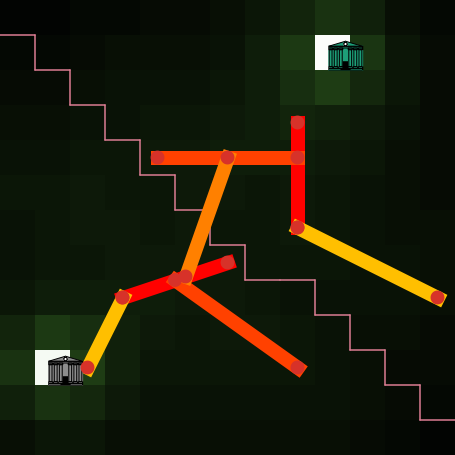
\includegraphics[width=0.5\textwidth]{Figures/PartII/Modeling/Lutecia/ex_collab_0}
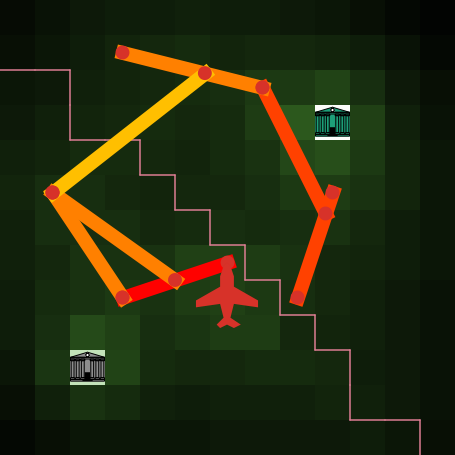
\includegraphics[width=0.5\textwidth]{Figures/PartII/Modeling/Lutecia/ex_dc_finalCollab}\\
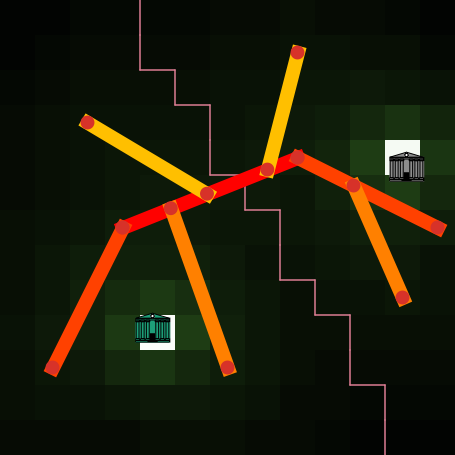
\includegraphics[width=0.5\textwidth]{Figures/PartII/Modeling/Lutecia/ex_simpleNash_0}
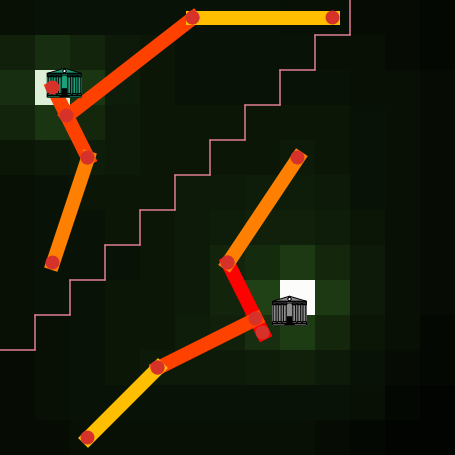
\includegraphics[width=0.5\textwidth]{Figures/PartII/Modeling/Lutecia/example_nocollab_0}
\caption[Examples of final configurations]{Examples of final configurations, with or without externality, for different values of cooperation parameters.}
\label{fig:luteciaexample}
\end{figure}
%%%%%%%%%%


%%%%%%%%%%
\begin{figure}
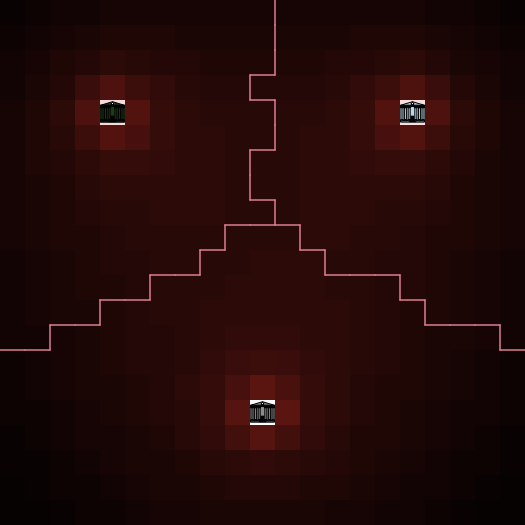
\includegraphics[width=0.5\textwidth]{Figures/PartII/Modeling/Lutecia/_MEAN_ACC}
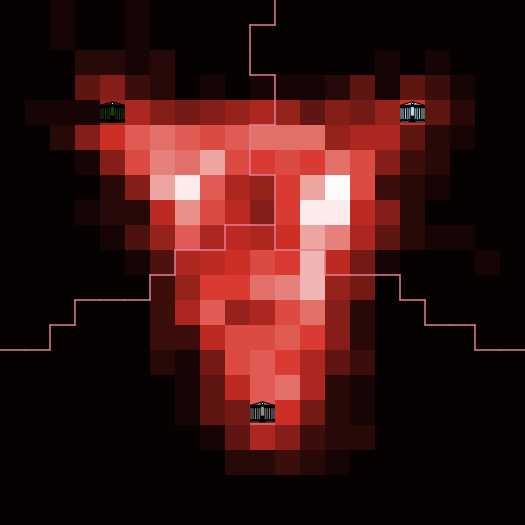
\includegraphics[width=0.5\textwidth]{Figures/PartII/Modeling/Lutecia/_NW_FREQ}
\caption[Validation of network exploration heuristic]{Validation of network exploration heuristic : mean accessibility(left) and network positions on 500 realizations on the same initial configuration. The optimal distribution of network validates network generation heuristic.}
\label{fig:luteciavalid}
\end{figure}
%%%%%%%%%%%



\subsubsection{Exploration and Validation}

We show in Fig.~\ref{fig:luteciaexample} and Fig.\ref{fig:luteciavalid} examples of obtained configurations and preliminary validation of governance and network growth heuristic. Internal validation and external validation through stylized facts, and model explorations, including statistical analysis of model behavior, are provisory for now and not presented here (see~\cite{le2015modeling} for preliminary results).


%\subsection{Perspectives}
% why is this model useful for the following













%% Chapter 3

\chapter{Math Test Chapter} % Chapter title

\label{ch:mathtest} % For referencing the chapter elsewhere, use \autoref{ch:mathtest}

%----------------------------------------------------------------------------------------

\lipsum[13]

%----------------------------------------------------------------------------------------

\section{Some Formulas}

Due to the statistical nature of ionisation energy loss, large fluctuations can occur in the amount of energy deposited by a particle traversing an absorber element\footnote{Examples taken from Walter Schmidt's great gallery: \\ \url{http://home.vrweb.de/~was/mathfonts.html}}.  Continuous processes such as multiple scattering and energy loss play a relevant role in the longitudinal and lateral development of electromagnetic and hadronic showers, and in the case of sampling calorimeters the measured resolution can be significantly affected by such fluctuations in their active layers.  The description of ionisation fluctuations is characterised by the significance parameter $\kappa$, which is proportional to the ratio of mean energy loss to the maximum allowed energy transfer in a single collision with an atomic electron: \graffito{You might get unexpected results using math in chapter or section heads. Consider the \texttt{pdfspacing} option.}
\begin{equation}
\kappa =\frac{\xi}{E_{\mathrm{max}}} %\mathbb{ZNR}
\end{equation}
$E_{\mathrm{max}}$ is the maximum transferable energy in a single collision with an atomic electron.
\[E_{\mathrm{max}} =\frac{2 m_{\mathrm{e}} \beta^2\gamma^2 }{1 + 2\gamma m_{\mathrm{e}}/m_{\mathrm{x}} + \left ( m_{\mathrm{e}} /m_{\mathrm{x}}\right)^2}\ ,\]
where $\gamma = E/m_{\mathrm{x}}$, $E$ is energy and $m_{\mathrm{x}}$ the mass of the incident particle, $\beta^2 = 1 - 1/\gamma^2$ and $m_{\mathrm{e}}$ is the electron mass. $\xi$ comes from the Rutherford scattering cross section and is defined as:
\begin{eqnarray*} \xi  = \frac{2\pi z^2 e^4 N_{\mathrm{Av}} Z \rho
\delta x}{m_{\mathrm{e}} \beta^2 c^2 A} =  153.4 \frac{z^2}{\beta^2}
\frac{Z}{A}
\rho \delta x \quad\mathrm{keV},
\end{eqnarray*}
where

\begin{tabular}{ll}
$z$ & charge of the incident particle \\
$N_{\mathrm{Av}}$ & Avogadro's number \\
$Z$ & atomic number of the material \\
$A$ & atomic weight of the material \\
$\rho$ & density \\
$ \delta x$ & thickness of the material \\
\end{tabular}

$\kappa$ measures the contribution of the collisions with energy transfer close to $E_{\mathrm{max}}$.  For a given absorber, $\kappa$ tends towards large values if $\delta x$ is large and/or if $\beta$ is small.  Likewise, $\kappa$ tends towards zero if $\delta x $ is small and/or if $\beta$ approaches $1$.

The value of $\kappa$ distinguishes two regimes which occur in the description of ionisation fluctuations:

\begin{enumerate}
\item A large number of collisions involving the loss of all or most of the incident particle energy during the traversal of an absorber.

As the total energy transfer is composed of a multitude of small energy losses, we can apply the central limit theorem and describe the fluctuations by a Gaussian distribution. This case is applicable to non-relativistic particles and is described by the inequality $\kappa > 10 $ (\ie, when the mean energy loss in the absorber is greater than the maximum energy transfer in a single collision).

\item Particles traversing thin counters and incident electrons under any conditions.

The relevant inequalities and distributions are $ 0.01 < \kappa < 10 $, Vavilov distribution, and $\kappa < 0.01 $, Landau distribution.
\end{enumerate}

%----------------------------------------------------------------------------------------

\section{Various Mathematical Examples}

If $n > 2$, the identity \[t[u_1,\dots,u_n] = t\bigl[t[u_1,\dots,u_{n_1}], t[u_2,\dots,u_n] \bigr]\] defines $t[u_1,\dots,u_n]$ recursively, and it can be shown that the alternative definition \[t[u_1,\dots,u_n] = t\bigl[t[u_1,u_2],\dots,t[u_{n-1},u_n]\bigr]\] gives the same result. % Chapter 4 - empty template

\cleardoublepage % Empty page before the start of the next part


%------------------------------------------------

\ctparttext{This concluding remark, for now a brief roadmap, is one objective of our thesis as implementation of our theory ans thus is expected to become a consequent part. We conclude here this preliminary work by perspectives and roadmap. This part make the synthesis of what was build until now, towards a delicate though robust edifice.}


% Part III : Towards operational models
%\part{Towards operational models}
\part{Synthesis}


%  A family of dynamic models : develop aim.

%  Various case studies : develop launched/potential collaborations




% introduction de la partie 

\section*{A Roadmap for an Operational Family of Models of Coevolution}{Vers des Modèles Opérationnels de Coevolution} % Chapter title

\label{ch:operational}

%----------------------------------------------------------------------------------------

As previously stated, one of our principal aims is the validation of the network necessity assumption, that is the differentiating point with a classic evolutive urban theory. To do so, toy-model exploration and empirical analysis will not be enough as hybrid models are generally necessary to draw effective and well validated conclusions. We briefly give an overview of planned work in the following, that will be the conclusion of this Memoire.



%----------------------------------------------------------------------------------------



\section*{Objectives}{Objectifs}


We expect to product \emph{models of coevolution}, \comment{(Florent) expliciter la différence avec ce que tu as fait jusque là}
 with the emphasis on processes of coevolution, to directly confront the theory. They will be necessary a flexible family because of the variety of scales and concrete cases we can include and we already began to explore in preliminary studies. Processes already studied can serve either as a thematic bases for a reuse as building bricks in a multi-modeling context, or as methodological tools such as synthetic data generator for synthetic control. Finally, we mean by operational models hybrid models, in the sense of semi-parametrized or semi-calibrated on real datasets or on precise stylized facts extracted from these same datasets. This point is a requirement to obtain a thematic feedback on geographical processes and on theory.


%----------------------------------------------------------------------------------------

\section*{Case Studies}{Cas d'étude}

Currently we expect to work on the following case studies to build these hybrid models :

\begin{itemize}
\item Dynamical data for Bassin Parisien should allow to parametrize and calibrate a model at this temporal and spatial scale.
\item On larger scales, South African dataset of \noun{Baffi} will along empirical analysis also be used to parametrize hybrid co-evolution models.
\item A possibility that is not currently set up (and that may however be difficult because of a disturbing closed-data policy among a frightening large number of scientists !) is the exploitation of French railway growth dataset (with population dataset) used in~\cite{bretagnolle:tel-00459720}, that would also provide an interesting case study on other regimes, scales and transportation mode.
\end{itemize}



%----------------------------------------------------------------------------------------



\section*{Roadmap}{Feuille de Route}


We give the following (non-exhaustive and provisory) roadmap for modeling explorations (theoretical and empirical domains being still explored conjointly) :

\begin{enumerate}
\item Complete the exploration of independent and weak coupled urban growth and network growth processes (all models presented in chapter~\ref{ch:modeling}), in order to know precisely involved mechanisms when they are virtually isolated, and to obtain morphogenesis scales.
\item Go further into the exploration of toy-model of non conventional processes such as governance network growth heuristic to pave the road for a possible integration of such modules in hybrid models.
\item Build a Marius-like generic infrastructure that implement the theory in a family of models that can be declined into diverse case studies.
\item Launch it and adapt it on these case studies.
\end{enumerate}

Next steps would be too hypothetical if formulated, we propose thus to proceed iteratively in our construction of knowledge and naturally update this roadmap constantly.

\bigskip
\bigskip
\bigskip

\textit{ - La route est longue mais la voie est libre.}










\cleardoublepage

%------------------------------------------------

\ctparttext{A building is never used the way it was designed, that is a reality which grasping makes the difference between good and excellent architects. The effective functional use give sense to any construction. So goes it for a knowledge edifice. We shall now take a look back on what we constructed and try to take a step back. This part develops first theoretical apparels emerging from the various aspects already tackled. It then proposes to extract fundamental open questions that future research on territorial complex systems will have to tackle in the incoming decades.}


% Opening
\part{Opening}
% TODO opening is not a good 
% this part should make a "meta-synthesis" (include here theories ? and research project for the future - lines of research and fundamental questions)


\cleardoublepage



%%%%%%%%%%%%%%%%%%%%%%%%%%%%%
% Chapter : Theoretical Framework



% Chapter 

\chapter{Theoretical Framework} % Chapter title

\label{ch:theory} % For referencing the chapter elsewhere, use \autoref{ch:name} 

%----------------------------------------------------------------------------------------



\headercit{Your theory is crazy, but not enough to be true.}{Niels Bohr}{}

\bigskip


Theory is a key element of any scientific construction, especially in Human Sciences in which object definition and questioning are more open but also determining for research directions. We develop in this chapter a self-consistent theoretical background. It naturally emerges from thematic considerations of previous chapter, empirical explorations done in chapter~\ref{ch:empirical} and modeling experiments conducted in chapter~\ref{ch:modeling}, as a linear structure of knowledge is not appropriate to translate the type of scientific entreprise we are conducting, typically in the spirit of \noun{Sanders} in~\cite{livet2010} for which the simultaneous conjonction of empirical, conceptual and modeling domains is necessary for the emergence of knowledge. This theoretical construction is however presented to be understood independently, and is used as a structuring skeleton for the rest of the thesis.

We propose first to construct the \emph{geographical theory} that will pose the studied objects and their meaning in the real world (their ontology), with their interrelations. This yields precise assumptions that will be sought to be confirmed or proven false in the following. Staying at a thematic level appears however to be not enough to obtain general guidelines on the type of methodologies and the approaches to use. More precisely, even if some theories imply an more natural use of some tools\footnote{to give a rough example, a theory emphasizing the complexity of relations between agents in a system will conduct generally to use agent-based modeling and simulation tools, whereas a theory based on macroscopic equilibrium will favorise the use of exact mathematical derivations.}, at the subtler level of contextualization in the sense of the approach taken to implement the theory (as models or empirical analysis), the freedom of choice may mislead into unappropriated techniques or questionings (see \cite{raimbault2016cautious} on the example of incautious use of big data and computation). We develop therefore in a second section a theoretical framework at a meta-level, aiming to give a vision and framing for modeling socio-technical systems.



%----------------------------------------------------------------------------------------

\newpage

% first section that develops elements of geographical theory : system of cities, territories, etc.
%  city morphogenesis ? -> link to other approaches of morphogenesis (Turing)
%  coevolution : give a precise theoretical meaning

% HERE precise exact definition, framed precisely (reference for the following).

\section{Geographical Theoretical Context}



%%%%%%%%%%%
\subsection{Foundation}



%%%%%%%%%%%%%%
\subsubsection{Networked Human Territories}

Our first pillar has already been constructed before in the thematic exploration of the research subject. We rely on the notion of \emph{Human Territory} elaborated by \noun{Raffestin} as the basis for a definition of territorial systems. It permits to capture complex human geographical systems in their concrete and abstract characteristics and representation. For example, a metropolitan territorial system can be apprehended simply by the functional extent of daily commuting, or by the perceived or lived space of different populations, the choice depending on the precise question asked. Note that this approach to territory is a position and that other (possibly compatible) entries could be taken~\cite{murphy2012entente}. The concrete of this pillar in reinforced by the territorial theory of networks of \noun{Dupuy}, yielding the notion of networked human territory, as a human territory in which a set of potential transactional networks have been realized, which is in accordance with vision of the territory as networked places~\cite{champollion:halshs-00999026}. We make therein the assumption that real networks are necessary elements of territorial systems.


%%%%%%%%%%%%%%%
\subsubsection{Evolutive Urban Theory}

% development of Denise theory
%  -> extension with precision on coevolution ? (read Holland on coevolution) -- beware of biological //

The second pillar of our theoretical construction is the Evolutive Urban Theory of \noun{Pumain}, closely linked to the complexity approach we take. This theory was first introduced in~\cite{pumain1997pour} which argues for a dynamical vision of city systems, in which self-organization is key. Cities are interdependent evolutive spatial entities whose interrelations produces the macroscopic behavior at the scale of city system. The city system is also designed as a network of city what emphasizes its view as a complex system. Each city is itself a complex system in the spirit of~\cite{berry1964cities}, the multi-scale aspect being essential in this theory, since microscopic agents convey system evolution through complex feedbacks between scales. The positioning within Complex System Sciences was later confirmed~\cite{pumain2003approche}. It was shown that this theory provide an interpretation for the origin of pervasive scaling laws, resulting from the diffusion of innovation cycles between cities~\cite{pumain2006evolutionary}. The aspect of resilience of system of cities, induced by the adaptive character of these complex systems, implies that cities are drivers and adapters of social change~\cite{pumain2010theorie}. Finally, path dependance yield non-ergodicity within these systems, making ``universal'' interpretations of scaling laws developed by physicists incompatible with evolutive urban theory~\cite{pumain2012urban}. We will interpret territorial systems following that idea of complex adaptive systems.




%%%%%%%%%%%
\subsubsection{Urban Morphogenesis}

% -> make a link between city systems and urban form/cityscape / territorial configurations

% Why morphogenesis is important : linked with modularity and scale -> if a submodule can be explained independantly (ie morphigeneis process is isolated), then we have the characteristic scale. then when size grows and interaction within city system -> can not explain alone (or with externalities ?) -> need a change in scale. ex. influecne of city system for size, activities; posiiton of an airport in a metropoltian region ; emergence of MCR.  ==> Assimptions to be tested with models ?.

% Alexander and Salingaros

% include transportation network, hierarchy and congestion in transport : Remy vs Benjamin (paper ? -> see with René)


The idea of morphogenesis was introduced by \noun{Turing} in~\cite{turing1952chemical} when trying to isolate simple chemical rules that could lead to the emergence of the embryo and its form. The morphogenesis of a system consists in self-consistent evolution rules that produce the emergence of its successives states, i.e. the precise definition of self-organization. Progresses towards the understanding of embryo morphogenesis (in particular the isolation of processes producing the differentiation of cells from an unique cell) has been made only recently with the use of Complexity Approaches in integrative biology~\cite{delile2016chapitre}. In the case of urban systems, the idea of urban morphogenesis, i.e. of self-consistent mechanisms that would produce the urban form, is more used in the field of architecture and urban design~\cite{hachi2013master} (as \noun{Alexander} generative grammar ``Pattern Language'' e.g.), in relation with theories of Urban Form~\cite{moudon1997urban}. This idea can be pushed into very small scales such as the building~\cite{whitehand1999urban} but we will use it more at a mesoscopic scale, in terms of land-use changes within an intermediate scale territorial system, in the same ontologies as Urban morphogenesis modeling literature (for example \cite{bonin2012modele} describes a model of urban morphogenesis with qualitative differentiation, whereas \cite{makse1998modeling} give a model of urban growth based on a mono-centric population distribution perturbed with correlated noises). The notion of morphogenesis will be important in our theory in link with modularity and scale. Modularity of a complex system consists in its decomposition into relatively independent sub-modules, and modular decomposition of a system can be seen as a way to disentangle non-intrinsic correlations~\cite{2015arXiv150904386K} (think of a block diagonalisation of a first order dynamical system). The isolation of a subsystem yields a corresponding characteristic scale. Isolating possible morphogenesis processes imply a controlled isolation (controlled boundary conditions e.g.) of the considered system, corresponding to a modularity level and thus a scale. When self-consistent processes are not enough to explain the evolution of the system (with reasonable action on boundary conditions), a change of scale is necessary, caused by an underlying phase transition in modularity. The example of metropolitan growth is a good example : complexity of interactions within the metropolitan region will grow with size and diversity of functions leading to a change in scale necessary to understand processes. The emergence of an international airport will strongly influence local development, what corresponds to the significant integration within a larger system. The characteristic scales and processes for which these change occur will be precise questions to be investigated through modeling. It is interesting to remark that a territorial subsystem in which morphogenesis has a sense can be seen as an \emph{autopoietic system} in the extended sense of \noun{Bourgine} in~\cite{bourgine2004autopoiesis}, as a network of auto-reproducing processes\footnote{which are however not cognitive, making this auto-organized systems fortunately not alive in the sense of autopoietic and cognitive systems} regulating their boundary conditions, what emphasizes boundaries on which we will last insist.


% transition : Bourgine autopoiesis -> importance of boundaries -> link to Holland.

%%%%%%%%%%%
\subsubsection{Co-evolution}

% other insight : Holland Signal and Boundaries, ecological niche etc. : contextualize within this framework, clarify definition of co-evolution

Our last pillar is a clarification of the notion of \emph{co-evolution}, on which \noun{Holland} shed light through an approach of complex adaptive systems by a theory of CAS as signal processing agents operating thanks to their boundaries~\cite{holland2012signals}. In this theory, complex adaptive systems form aggregates at diverse hierarchical levels, that correspond to different level of self-organization, and boundaries are vertically and horizontally intricate in a complex way. That approach introduces the notion of \emph{niche} as a relatively independent subsystem in which ressources circulate (the same way as network communities) : numerous illustrations are given such as economical niches or ecological niches. Agents within a niche are said to be \emph{co-evolving}. Co-evolution thus means strong interdependences (implying circular causal processes) and a certain independence regarding the exterior of the niche. The notion is naturally flexible as it will depend on ontologies, resolution, thresholds etc. considered to define the system. This concept is easily transmissible to the evolutive urban theory and converges with the notion of co-evolution described by \noun{Pumain} : co-evolving agents in a system of cities consist in a niche with its flows, signals and boundaries and thus co-evolving entities in the sense of \noun{Holland}. This notion will be important for us in the definition of territorial subsystems and their coupling.



%%%%%%%%%%%
%\subsection{Requirements}
% RQ : no requirements for the theory, contained within pillars : requirement is the presence of these pillars ?



%%%%%%%%%%%
\subsection{Synthesis : an theory of co-evolutive networked territorial systems}

% put different elements together and construct the geographical theory
% give here precise definitions

We synthesize our pillars as a short self-consistent geographical theory of territorial systems in which networks play a central role in the co-evolution of components of the system. See the foundation subsection for definitions and references. The formulation is intended to be minimalistic.

\medskip

\begin{definition}
\textbf{ - Territorial System.} A territorial system is a set of networked human territories, i.e. human territories in and between which real networks exist.
\end{definition}

\medskip

At this step complexity and dynamical evolutive characters of territorial systems are implied but not an explicit part of the theory. We will assume to simplify a discrete definition of temporal, spatial and ontological scales under modularity and local stationarity assumptions.

% definition of scale and stationarity
%\textit{Equivalence between existence of discrete scales and discrete stationarity levels ?}

\medskip

\begin{proposition}
\textbf{ - Discrete scales.} Assuming a discrete modular decomposition of a territorial system, the existence of a discrete set $(\tau_i,x_i)$ of temporal and functional scales for the territorial system is equivalent to the local temporal stationarity of a random dynamical system specification of the system.
\end{proposition}

\begin{proof}
\textbf{(Sketch of).} We underlie that any territorial system can be represented by random variables, what is equivalent to have well defined objects and states and use the Transfer Theorem on events of successive states. If $X=(X_j)$ is the modular decomposition, we have necessarily quasi-independence of components in the sense that $\Covb{dX_j}{dX_{j'}}\simeq 0$ at any time. General stationarity transitions induce modular transitions that are kept or not depending if they correspond to an effective transition within the subsystem, what provide temporal scales as characteristic times of sub-dynamics. Functional scales are the corresponding extent in the state space.\qed
\end{proof}

% assumption : existence of scales

\medskip

This proposition induce a discrete representation of system dynamics in time. Note that even in the case of no modular representation, the system as a whole will verify the property. This definition of scales allows to explicitly introduce feedback loops and thus emergence and complexity, making our theory compatible with the evolutive urban theory.



\begin{assumption}
\textbf{ - Scales and Subsystems intrication. } Complex networks of feedbacks exist both between and inside scales, what impose the existence of weak emergence~\cite{bedau2002downward}. Furthermore a horizontal and vertical hierarchical imbrication of boundaries is not the rule.
\end{assumption}

% co-evolution

Within these complex subsystems intrications we can isolate co-evolving components using morphogenesis. The following proposition is a consequence of the equivalence between the independence of a niche and its morphogenesis. Morphogenesis provides the modular decomposition (local stationarity assumed) needed for the existence of scale, giving minimal vertically (scale) and horizontally (space) independent subsystems.

\begin{proposition}
\textbf{ - Co-evolution of components. } Morphogenesis processes of a territorial system are an equivalent formulation of the existence of co-evolutive subsystems.
\end{proposition}


% importance of nws as necessary subcomponents
%  maybe where we diverge from Denise theory ?

Finally we make a key assumption putting real networks at the center of co-evolutive dynamics, introducing their necessity to explain dynamical processes of territorial systems.

\begin{assumption}
\textbf{ - Necessity of Networks. } Network evolution can not be explained only by the dynamics of other territorial components and reciprocally, i.e. co-evolving territorial subsystems include real networks. They can thus be at the origin of regime changes (transition between stationarity regimes) or more dramatic bifurcations in dynamics of the whole territorial system.
\end{assumption}

On long time scale, an overall co-evolution has been shown for the french railway network by~\cite{bretagnolle:tel-00459720}. At smaller scales it is less evident (debate on structural effects) but we postulate that co-evolution effects are present at any scale. Regional examples may illustrate that : Lyon has not the same dynamical relations with Clermont than with Saint-Etienne and network connectivity has necessarily a role in that (among intrinsic interaction dynamics and distance). At a smaller scale, we think that effects are even less observable, but precisely because of the fact that co-evolution is stronger and local bifurcations will occur with stronger amplitude ans greater frequency than in macroscopic systems where attractors are more stable and stationarity scales greater. We will try to identify bifurcation or phase transitions in toy models, hybrid models and empirical analysis, at different scales, on different case studies and with different ontologies.

One difficulty in our construction is the stationarity assumption. Even if it seems a reasonable assumptions on large scales and has already been observed in empirical data~\cite{sanders1992systeme}, we shall verify it in our empirical studies. Indeed, this question is at the center of current research efforts to apply deep learning techniques to geographical systems : \noun{Bourgine} has recently developed a framework to extract patterns of Complex Adaptive Systems\footnote{Using a representation theorem~\cite{knight1975predictive}, any discrete stationary process is a \emph{Hidden Markov Model}. Given the definition of a causal state as $\Pb{future | A} = \Pb{future | B}$, the partition of system states induced by the corresponding equivalence relations allows to derive a \emph{Recurrent Network} that is enough to determine next state of the system, as it is a \emph{deterministic} function of previous state and hidden states~\cite{shalizi2001computational} : $(x_{t+1},s_{t+1}) = F\left[(x_t,s_t)\right]$. The estimation of Hidden States and of the Recurrent Function thus captures through deep learning entirely dynamical patterns of the system, i.e. full information on its dynamics and internal processes.}. The issues are then if the stationarity assumption be tackled through augmentation of system states, and if heterogeneous and asynchronous data be used to bootstrap long time-series necessary for a correct estimation of the neural network. These issue are related to the stationarity assumption for the first and to non-ergodicity for the second.




%----------------------------------------------------------------------------------------

\newpage

\section{A theoretical Framework for the Study of Socio-technical Systems}

After having set up the thematic theoretical framework, we develop a more general framework in which the previous can enter. At an epistemological level, it is essential to frame generally our directions of research.


\subsection{Introduction}

\subsubsection*{Scientific Context}


% this part may rather be in introduction ? -> ok here as explains for why this meta-framework is needed.

The structural misunderstandings between Social Sciences and Humanities on one side, and so-called Exact Sciences on the other side, far from being a generality, seems to have however a significant impact on the structure of scientific knowledge~\cite{2015arXiv151103981H}. In particular, the place of theory (and indeed the signification of this term itself) in the elaboration of knowledge has a totally different place, partly because of the different \emph{perceived complexities}\footnote{We used the term \emph{perceived} as most of systems studied by physics might be described as simple whereas they are intrinsically complex and indeed not well understood~\cite{laughlin2006different}.} of studied objects : for example, mathematical constructions and by extent theoretical physics are \emph{simple} in the sense that they are mostly entirely analytically solvable, whereas Social Science subjects such as humans or society (to give a \emph{clich{\'e}} exemple) are \emph{complex} in the sense of complex systems\footnote{for which no unified definition exists but of which fields of application range broadly from neuroscience to quantitative finance, including e.g. quantitative sociology, quantitative geography, integrative biology, etc.~\cite{newman2011complex}, and for which study various complementary approaches may be applied, such as Dynamical Systems, Agent-based Modeling, Random Matrix Theory}, thus a stronger need of a constructed theoretical (generally empirically based) framework to identify and define the objects of research that are necessarily more arbitrary in the framing of their boundaries, relations and processes, because of the multitude of possible viewpoints : Pumain suggests indeed in~\cite{pumain2005cumulativite} a new approach to complexity deeply rooted in social sciences that ``would be measured by the diversity of disciplines needed to elaborate a notion''. These differences in backgrounds are naturally desirable in the spectrum of science, but things can get nasty when playing on ``common'' terrains, typically complex systems problematics as already detailed, as the exemple of geographical urban systems has recently shown~\cite{dupuy2015sciences}. Complex System Science\footnote{that we deliberately call that way although there is a running debate on wether it can be seen as a Science in itself or more as a different way to do Science.} is presented by some as a ``new kind of Science''~\cite{wolfram2002new}, and would at least be a symptom of a shift in scientific practices, from analytical and ``exact'' approaches to computational and evidence-based approaches~\cite{arthur2015complexity}, but what is sure is that it brings, together with new methodologies, new scientific fields in the sense of converging interests of various disciplines on transversal questions or of integrated approaches on a particular field~\cite{2009arXiv0907.2221B}.



\subsubsection*{Objectives}

Within that scientific context, the study of what we will call \emph{Socio-technical Systems}, which we define in a rather broad way as hybrid complex systems including social agents or objects that interact with technical artifacts and a natural environment\footnote{geographical systems in the sense of \cite{dollfus1975some} are the archetype of such systems, but that definition may cover other type of systems such as an extended transportation system, social systems taken with an environmental context, complicated industrial systems taken with users, etc.}, lies precisely between social sciences and hard sciences. The example of Urban Systems is the best example, as already before the arrival of approaches claiming to be ``more exact'' than soft approaches (typically by physicists, see e.g. the rather disturbing introduction of~\cite{louf2014scaling}, but also by scientists coming from social sciences such as Batty~\cite{batty2013new}), many aspects of urban systems were already in the field of exact sciences, such as urban hydrology, urban climatology or technical aspects of transportation systems, whereas the core of their study relied in social sciences such as geography, urbanism, sociology, economy. Therefore a necessary place of theory in their study : following~\cite{livet2010}, the study of complex systems in social science is an interaction between empirical analysis, theoretical constructions, and modeling.

We propose in this paper to construct a theory, or rather a theoretical framework, that would ease some aspects of the study of such systems. Many theories already exist in all fields related to this kind of problems, and also at higher levels of abstraction concerning methods such as agent-based modeling e.g., but there is to our knowledge no theoretical framework including all of the following aspects that we consider as being crucial (and that can be understood as an informal basis of our theory) :
% QUESTION : do we need to include here empirical examples to support these claims ? - or are there taken as granted, the theoretical basis (that indeed comes from empirical practice)?
\begin{enumerate}
\item a precise definition and emphasis on the notion of coupling between subsystems, in particular allowing to qualify or quantify a certain degree of coupling : dependence, interdependence, etc. between components.
\item a precise definition of scale, including timescale and scales for other dimensions.
\item as a consequence of the previous points, a precise definition of what is a system.
\item the inclusion of the notion of emergence in order to capture multi-scale aspects of systems.
\item a central place of ontology in the definition of systems, i.e. of the sense in the real world given to its objects\footnote{\textit{as already explained before, this positioning along with the importance of structure may be related to Ontic Structural Realism~\cite{frigg2011everything} in further in further developments.}
}.
\item taking into account heterogeneous aspects of the same system, that could be heterogeneous components but also complementary intersecting views.
\end{enumerate}


The rest of this section is organized as follows : we construct the theory in the following part, staying at an abstract level, and propose a first application to the question of co-evolving subsystems. We then discuss positioning regarding existing theories, and possible developments and concrete applications.


\subsection{Construction of the theory}

\subsubsection*{Perspectives and Ontologies}

The starting point of the theory construction is a perspectivist epistemological approach on systems introduced by Giere~\cite{giere2010scientific}.  To sum up, it interprets any scientific approach as a perspective, in which someone pursues some objective and uses what is called \emph{a model} to reach it. The model is nothing more than a scientific medium. Varenne developed~\cite{varenne2010framework} model typologies that can be interpreted as a refinement of this theory. Let for now relax this possible precision and use perspectives as proxies of the undefined objects and concepts. Indeed, different views on the same object (being complementary or diverging) have the property to share at least the object in itself, thus the proposition to define objects (and more generally systems) from a set of perspectives on them, that verify some properties that we formalize in the following.

A perspective is defined in our case as a dataflow machine $M$ (that corresponds to the model as medium) in the sense of~\cite{golden2012modeling} that gives a convenient way to represent it and to introduce timescales, to which is associated an ontology $O$ in the sense of~\cite{livet2010}, i.e. a set of elements each corresponds to a \emph{thing} (it can be an object, an agent, a process, etc.) % better word than ``thing'' ? seems appropriate as can be object, agent, process, etc.
 in the real world. We include only two aspect (the model and the objects represented) of Giere's theory, making the assumption that purpose and user of the perspective are indeed contained in the ontology.

\begin{definition}
A \emph{perspective on a system} is given by a dataflow machine $M = (i,o,\mathbb{T})$ and an associated ontology $O$. We assume that the ontology can be decomposed into atomic elements $O=(O_j)_j$.
\end{definition}

The atomic elements of the ontology can be particular elements such as agents or components of the system, but also processes, interactions, states, or concepts for example. The ontology can be seen as the rigorous description of the content of the perspective. The assumption of a dataflow machine implies that possible inputs and outputs can be quantified, what is not necessarily restrictive to quantitative perspectives, as most of qualitative approaches can be translated into discrete variables as long as the set of possibles is known or assumed. 

The system is then defined ``reversely'', i.e. from a set of perspectives on a system :

% def of a system as a set of perspectives.
\begin{definition}
A \emph{system} is a set of \emph{perspectives on a system} : $S = (M_i,O_i)_{I\in I}$, where $I$ may be finite or not.
\end{definition}

We denote by $\mathcal{O} = (O_{j,i})_{j,i\in I}$ the set of all elements within ontologies.

Note that at this level of construction, there is not necessarily any structural consistence in what we call a system, as given our broad definition could allow for example to consider as a system a perspective on a car together with a perspective on a system of cities what makes reasonably no sense at all. Further definitions and developments will allow to be closer from classical definition of a system (interacting entities, designed artifacts, etc.). The same way, the definition of a subsystem will be given further. The introduced elements of our approach help to tackle so far points three, five and six of the requirements.

\paragraph{Precision on the recursive aspect of the theory}

One direct consequence of these definitions must be detailed : the fact that they can be applied recursively. Indeed, one could imagine taking as perspective a system in our sense, therefore a set of perspectives on a system, and do that at any order. If ones takes a system in any classical sense, then the first order can be understood as an epistemology of the system, i.e. the study of diverse perspectives on a system. A set of perspectives on related systems may in some conditions be a domain or a field, thus a set of perspectives on various related systems the epistemology of a field. These are more analogies to give the idea behind the recursive character of the theory. It is indeed crucial for the meaning and consistence of the theory because of the following arguments :
\begin{itemize}
\item The choice of perspectives in which a system consists is necessarily subjective and therefore understood as a perspective, and a perspective on a system if we are able to build a general ontology.
\item We will use relations between ontologies in the following, which construction based on emergence is also subjective and seen as perspectives.
\end{itemize}



\subsubsection*{Ontological Graph}

% construction of the ontological graph / canonical tree decomposition
%  : pb with relation in the ontological graph : weak or strong emergence ?

We propose then to capture the structure of the system by linking ontologies. This approach could eventually be linked to structural realism epistemological positioning~\cite{frigg2011everything} as knowledge of the world is partly contained here in structure of models. % precise here epistemological positioning, we may be clearly within a structural realist positioning !!
 Therefore, we choose to emphasize the role of emergence as we believe that it may be one practical minimalist way to capture quite well complex systems structure\footnote{what of course can not been presented as a provable claim as it depends on system definition, etc.}. We follow on that point the approach of Bedau on different type of emergences, in particular his definition of weak emergence given in~\cite{bedau2002downward}. Let recall briefly definitions we will use in the following. Bedau starts from defining emerging properties and then extends it to phenomena, entities, etc. The same way, our framework is not restricted to objects or properties and wrapped thus the generalized definitions into emergence between ontologies. We will apply the notion of emergence under the two following forms\footnote{the third form Bedau recalls, \emph{Strong emergence} will not be used, as we need only to capture dependance and autonomy, and weak emergence is more satisfying in terms of complex systems, as it does not assume ``irreducible causal powers'' to the greater scale objects. Nominal emergence is used to capture inclusion between ontologies.} :
\begin{itemize}
\item \emph{Nominal emergence} : one ontology $O'$ is included in an other $O$ but the aspect of $O$ that is said to be nominally emergent regarding $O'$ does not depend on $O'$.
\item \emph{Weak emergence} : one part of an ontology $O$ can be derived by aggregation of elements and interactions between elements of an ontology $O'$.
\end{itemize}

As developed before, the presence of emergence, and especially weak emergence, will consist in itself in a perspective. It can be conceptual and postulated as an axiom within a thematic theory, but also experimental if clues of weak emergence are effectively measured between objects. In any case, the relation between ontologies must be encoded within an ontology, which was not necessarily introduced in the initial definition of the system.


% Observation : -
%  - Ontologies are sets -> relation between subsets.
%  - include emergence relations between different perspectives of the system ? would imply a coupling ontology ? -> YES - system is not only a set but also a relation between its elements -> introduce the 'coupling ontology' ; or assumes there exists one ?

We make therefore the following assumption for next developments :
\begin{assumption}
A system can be partially structured by extending it with an ontology that contains (not necessarily only) relations between elements of ontologies of its perspectives. We name it the \emph{coupling ontology} and assume its existence in the following. We assume furthermore its atomicity, i.e. if $O$ is in relation with $O'$, then any subsets of $O,O'$ can not be in relation, what is not restrictive as a decomposition into several independent subsets ensures it if it is not the case.
\end{assumption}

It allows to exhibit emergence relations not only within a perspective itself but also between elements of different perspectives. We define then pre-order relations between subsets of ontologies : % check pre-order and equivalence relations.

% order relations between ontologies
% first recall Bedau's paper. 
% check equivalence relation ; pre-order <- relations are only pre-order ?
\begin{proposition}
The following binary relationships are pre-orders on $\mathcal{P(O)}$ :
\begin{itemize}
\item Emergence (based on Weak Emergence) : $O' \preccurlyeq O$ if and only if $O$ weakly emerges from $O'$.
\item Inclusion (based on Nominal Emergence) : $O' \Subset O$ if and only if $O$ nominally emerges from $O'$.
\end{itemize}
\end{proposition}

\begin{proof}
With the convention that it can be said that an object emerges from itself, we have reflexivity (if such a convention seems absurd, we can define the relationships as \emph{$O$ emerges from $O'$ or $O=O'$ }). Transitivity is clearly contained in definitions of emergence.
\end{proof}

\medskip

Note that the inclusion relation is more than an inclusion between sets, as it translates an inclusion ``inside'' the elements of the ontology.

These relations are the basis for the construction of a graph called the \emph{ontological graph} :

% definition of the ontological graph
% ! beware to put only neighbor relations within the graph
% and to reconstruct by induction subsets at any level ?
\begin{definition}
The {ontological graph} is constructed by induction the following way :
\begin{enumerate}
\item A graph with vertices elements of $\mathcal{P(O)}$ and edges of two types : $E_W = \{(O,O') | O' \preccurlyeq O \}$ and $E_N = \{(O,O') | O' \Subset O \}$
\item Nodes are reduced\footnote{the reduction procedure aims to delete redundancy, keeping an entity at the higher level it exists.} by : if $o \in O,O'$ and ($O' \preccurlyeq O$ or $O' \Subset O$) but not ($O \preccurlyeq O'$ or $O \Subset O'$), then $O' \leftarrow O' \setminus o$
\item Nodes with intersecting sets are merged, keeping edges linking merged nodes. This step ensures non-overlapping nodes.
\end{enumerate}
\end{definition}


% definition of a subsystem in the large sense ? -> done after treeing the graph
% can be done only if reconstruction is possible.



\subsubsection*{Minimal Ontological Tree}

% theorem : tree construction with the tree-bag decomposition theorem ; and show trivially that loops are at the same scale
% first get a connected component of the graph -> here the consistence is captured : if ontologies have nothing to do at all, then it cant be the same system.

The topological structure of the graph, that contains in a way the \emph{structure of the system}% positioning regarding structural realism.
, can be reduced into a minimal tree that contains hierarchical structure essential to the theory.

We need first to give consistence to the system :

\begin{definition}
A consistent part of the ontological graph is a weakly connected component of the graph. We assume for now to work on a consistent part.
\end{definition}

% rq : consistent system ? -> would need to reconstruct perspectives ? possible ? under certain assumption ? 'decoupling ontology' ? -> need to be worked harder.

The notion of consistent system, together with subsystem or nodes timescales that will be defined later, requires to reconstruct perspectives from ontological elements, i.e. the inverse operation of what was done in our deconstruction procedure.

\begin{assumption}
There exists $\mathcal{O}' \subset \mathcal{P(O)}$ such that for any $O \subset \mathcal{O}'$, there exists a corresponding dataflow machine $M$ such that the corresponding perspective is consistent with initial elements of the system (i.e. machines on ontology overlaps are equivalent). If $\Phi : M \mapsto O$ is the initial mapping, we denote this extended reciprocal construction by $M' = \Phi^{<-1>}(O)$.
\end{assumption}

\paragraph{Remark.}

This assumption could eventually be changed into a provable proposition, assuming that the coupling ontology is indeed a coupling perspective, which dataflow machine part is consistent with coupled entities. Therein, the decomposition postulate of~\cite{golden2012modeling} should allow to identify basic components corresponding to each element of the ontology, and then construct the new perspective by induction. We find however these assumptions too restrictive, as for example various ontological elements may be modeled by an irreducible machine, as a differential equations with aggregated variables. We prefer to be less restrictive and postulate the existence of the reverse mapping on some sub-ontologies, that should be in practice the ones where couplings can be effectively modeled.

Given this assumption, we can define the consistent system as the reciprocal image of the consistent part of the ontological graph. It ensures system connectivity what is a requirement for tree construction.

\begin{proposition}
The tree decomposition of the ontological graph in which nodes contains strongly connected components is unique. The corresponding reduced tree, that corresponds to the ontological graph in which strongly connected components have been merged with edges kept, is called the \emph{Minimal Ontological Tree}.
\end{proposition}

\begin{proof}
(sketch of) The unicity is obtained as nodes are fixed as strongly connected components. It is trivially a tree decomposition (with no edges) as in a directed graph, strongly connected components do not intersect, thus the consistence of the decomposition.
\end{proof}

Any loop $O \rightarrow O' \rightarrow \ldots \rightarrow O$ in the ontological graph assumes that all its elements are equivalent in the sense of $\preccurlyeq$. This equivalence loops should help to define the notion of strong coupling as an application of the theory (see applications).

\medskip

The Minimal Ontological Tree (MOT) is a tree in the undirected sense but a forest in the directed sense. Its topology contains a sort of system hierarchy. Consistent subsystems are defined from the set $\mathcal{B}$ of branches of the forest, as $(\Phi^{<-1>}(\mathcal{B}),\mathcal{B})$. The timescale of a node, and by extension of a subsystem, is the union of timescales of corresponding machines. Levels of the tree are defined from root nodes, and the emergence relations between nodes implies a vertical inclusion between timescales.



% check shortcuts reduction in graph construction : if O < O' < O'' , then O -> O'' is not an edge, must take the longest path.



\subsubsection*{Scales}

Finally, we propose to define scales associated to a system. Following~\cite{manson2008does}, an epistemological continuum of visions on scale is a consequence of differences between disciplines in the way we developed in the introduction. This proposition is indeed compatible with our framework, as the construction of scales for each level of the ontological tree results in a broad variety of scales.

Let $(M,O)$ a subsystem and $\mathbb{T}$ the corresponding timescale. We propose to define the ``thematic scale'' (for example spatial scale) assuming a representation theorem, i.e. that an aspect (thematic aspect) of the machine can be represented as a dynamic state variable $\vec{X}(t)$. Assuming a scale operator\footnote{that can be of various nature : extent, probabilistic extent, spectral scales, stationarity scales, etc.} $\norm{\cdot}_{S}$ and that the state variable has a certain level of differentiability, the \emph{thematic scale} if defined as $\norm{(d^k \vec{X}(t))_k}_S$


\subsection{Application}

\subsubsection*{The particular case of geographical systems}


%%
%  Observation :
%   ontologies could evolve in time ? they do -> cf Lucie's framework on spatio-temporal functional decomposition : each atomic unit can have a different ontology. not an issue : connects ontologies through a superior layer representing the object through all temporal extent ; the object nominally emerges from each temporal ontology.


In \cite{dollfus1975some} % ~ same def of system ; introduce structure in context ? link to explanation ?
 \noun{Durand-Dast{\`e}s} proposes a definition of geographical structure and system, structure would be the spatial container for systems viewed as complex open interacting systems (elements with attributes, relations between elements and inputs/outputs with external world). For a given system, its definition is a perspective, completed by structure to have a system in our sense. Depending on the way to define relations, it may be easy to extract ontological structure.
 %\textit{Note : find typical emergence clues in standard relational formalizations ? would guide the application of the theory.}


\subsubsection*{Modularity and co-evolving subsystems}


For the example of Urban Systems, urban evolutionary theory enters this framework using our previous thematic theory? The decomposition into uncorrelated subsystems yields precisely strongly coupled components as co-evolving components. The correlation between subsystems should be positively correlated with topological distance in the tree. If we define elements of a node before merging as \emph{strongly coupled elements}, in the case of dynamic ontologies, it provides a definition of \emph{co-evolution} and co-evolving subsystems equivalent to the thematic definition.


\subsection{Discussion}


\paragraph{Link with existing frameworks}

A link with the Cottineau-Chapron framework for multi-modeling~\cite{10.1371/journal.pone.0138212} may be done in the case they add the bibliographical layer, which would correspond to the reconstruction of perspectives. \cite{reymond2013logique} proposes the notion of ``interdisciplinary coupling'' what is close to our notion of coupling perspectives. A correspondance with System of Systems approaches (see e.g. \cite{luzeaux2015formal} for a recent general framework englobing system modeling and system description) may be also possible as our perspectives are constructed as dataflow machines, but with the significant difference that the notion of emergence is central.


\paragraph{Contributions to the study of complex systems}

\begin{itemize}
\item We do not claim to provide a theory of systems (beware of cybernetics, systemics etc. that could not model everything), but more a framework to guide research questions (e.g. in our case the direct outcomes will be quantitative epistemology that comes from system construction as perspectives research ; empirical to construct robust ontologies for perspectives ; targeted thematic to unveil causal relationship/emergence for construction of ontological network ; study of coupling as possible processes containing co-evolution ; study of scales ; etc.). It may be understood as meta-theory which application gives a theory, the thematic theory developed before being a specific implementation to territorial networked systems.
\item We Emphasize the notion of socio-technical system, crossing a social complex system approach (ontologies) with a description of technical artifacts (dataflow machines), taking the ``best of both worlds''.
\end{itemize}




\subsection{Research Directions}

We can draw from the construction of this theoretical framework a set of research directions, that give a general line on how trying to answer to research questions asked after the thematic theory construction.

\begin{enumerate}
\item The perspectivist approach implies a broad understanding of existing perspectives on a system, and of possibility of coupling between them ; thus an emphasis on applied epistemology, i.e. \textbf{Algorithmic Systematic Review} (exploration of the knowledge space), \textbf{Disciplines Mapping}(extraction of its structure) and \textbf{Datamining for Content Analysis}(refinement at the atomic level in scientific knowledge) that correspond to the three sections of chapter~\ref{ch:quantepistemo}.
\item At a finer level of particularization, the knowledge of perspectives means \textbf{Knowledge of stylized facts}, i.e. empirical analysis of cases studies. These are the object of chapter~\ref{ch:empirical}.
\item The emphasis on coupled subsystems at different scales implies a deep understanding of coupling mechanisms, thus the need of methodological and technical developments : \textbf{Methods for Statistical Control}, \textbf{Methods for Model Exploration}, \textbf{Theoretical Study of Coupling}, \textbf{Multi-Modeling}, of which some are developed and other proposed in the methodological chapter~\ref{ch:methodology}.
\item Furthermore, the possibility of hidden elements within the ontology implies the test for causal relations and intermediate processes at the origin of emergence, thus e.g. the exploration of new paradigms such as role of governance within complex models as done in chapter~\ref{ch:complexmodels}.
\item Finally, the idea behind system structure contained within the ontological forest is a large set of coupled models for a given system : it means that a proper system definition (i.e. thematic problematization and exploration) and construction should yield to a structured family of models : parallel branches can be different implementations of the same process or various processes trying to explain the emerging ontology ; therefore the final objective of a family of models tackling the thematic question.
\end{enumerate}











%%%%%%%%%%%%%%%%%%%%%%%%%%%%%




%------------------------------------------------

%\ctparttext{}


% Conclusion
%\part*{Conclusion}





%------------------------------------------------
% Provisory chapters 





%------------------------------------------------
% Bibliography


\cleardoublepage
% Bibliography

\label{app:bibliography} % Reference the bibliography elsewhere with \autoref{app:bibliography}

\manualmark % Work-around to have small caps also here in the headline
\markboth{\spacedlowsmallcaps{\bibname}}{\spacedlowsmallcaps{\bibname}} % Work-around to have small caps also
\phantomsection
\refstepcounter{dummy}

\addtocontents{toc}{\protect\vspace{\beforebibskip}} % Place the bibliography slightly below the rest of the document content in the table of contents
\addcontentsline{toc}{chapter}{\tocEntry{\bibname}}



\printbibliography % Bibliography



%----------------------------------------------------------------------------------------
%	THESIS CONTENT - APPENDICES
%----------------------------------------------------------------------------------------

%\appendix

\part{Appendix} % New part of the thesis for the appendix


%%%%%%%%%%%%%%%%%%
%% Appendix : Synthetic Data (introduction and financial development)

\chapter{Generation of Correlated Synthetic Data} % Chapter title

\label{app:syntheticdata} % For referencing the chapter elsewhere, use \autoref{ch:name} 

%----------------------------------------------------------------------------------------







 % provisory
%%%%%%%%%%%%%%%%%%

%%%%%%%%%%%%%%%%%%
%% Appendix : Morphogenesis

\chapter{An Interdisciplinary Approach to Morphogenesis} % Chapter title

\label{app:syntheticdata} % For referencing the chapter elsewhere, use \autoref{ch:name} 

%----------------------------------------------------------------------------------------

\textit{This Appendix was submitted as an Essay Paper with C. Antelope (U. California), L. Hubatsch (F. Crick Institute) and J.M. Serna (Université Paris 7), as : }

\noindent Antelope, C., Hubatsch, L., Raimbault, J., and Serna, J. M. (2016). An interdisciplinary approach to morphogenesis. \textit{Forthcoming in Proceedings of Santa Fe Institute CSSS 2016.}





 % provisory
%%%%%%%%%%%%%%%%%%



%%%%%%%%%%%%%%%%%%
%% Appendix : technical developments
\chapter{Technical Developments} % Chapter title

\label{app:technical} % For referencing the chapter elsewhere, use \autoref{ch:name} 

%----------------------------------------------------------------------------------------






\section{Derivations for Urban Growth Models}





\begin{lemma}
The limit of a Preferential Attachment model when $\lambda \ll 1$ is a linear-growth Gibrat model, with limit parameters $\mu_i(t)=1+\frac{\lambda}{m\cdot (t-1)}$.
\end{lemma}

\begin{proof}

Starting with first moment, we denote $\bar{P}_i(t)=\Eb{P_i(t)}$. Independence of Gibrat growth rate yields directly $\bar{P}_i(t)=\Eb{R_i(t)}\cdot \bar{P}_i(t-1)$. Starting for the preferential attachment model, we have $\bar{P}_i(t) = \Eb{P_i(t)} = \sum_{k=0}^{+\infty}{k\Pb{P_i(t)=k}}$. But
\[
\{P_i(t)=k\}=\bigcup_{\delta=0}^{\infty}{\left(\{P_i(t-1)=k-\delta\}\cap \{P_i\leftarrow P_i + 1\}^{\delta}\right)}
\]

where the second event corresponds to city $i$ being increased $\delta$ times between $t-1$ and $t$ (note that events are empty for $\delta \geq k$). Thus, being careful on the conditional nature of preferential attachment formulation, stating that $\Pb{\{P_i\leftarrow P_i + 1\} | P_i(t-1)=p} = \lambda\cdot\frac{p}{P(t-1)}$ (total population $P(t)$ assumed deterministic), we obtain

\begin{equation*}
\begin{split}
\Pb{\{P_i\leftarrow P_i + 1\}} & = \sum_{p}{\Pb{\{P_i\leftarrow P_i + 1\} | P_i(t-1)=p}\cdot \Pb{P_i(t-1)=p}}\\
&=\sum_{p}{\lambda\cdot\frac{p}{P(t-1)}\Pb{P_i(t-1)=p}}=\lambda\cdot\frac{\bar{P}_i(t-1)}{P(t-1)}\\
\end{split}
\end{equation*}

It gives therefore, knowing that $P(t-1)=P_0 + m\cdot (t-1)$ and denoting $q=\lambda\cdot\frac{\bar{P}_i(t-1)}{P_0 + m\cdot (t-1)}$

\[
\begin{split}
\bar{P}_i(t) & =\sum_{k=0}^{\infty}{\sum_{\delta=0}^{\infty}{k\cdot \left(\lambda\cdot\frac{\bar{P}_i(t-1)}{P_0 + m\cdot (t-1)}\right)^{\delta}\cdot \Pb{P_i(t-1)=k-\delta}}}\\
& = \sum_{\delta^{\prime}=0}^{\infty}{\sum_{k^{\prime}=0}^{\infty}{\left(k^\prime + \delta^{\prime}\right)\cdot q^{\delta^{\prime}} \cdot \Pb{P_i(t-1)=k^\prime}}}\\
& = \sum_{\delta^{\prime}=0}^{\infty}{q^{\delta^{\prime}}\cdot \left(\delta^{\prime} + \bar{P}_i(t-1)\right)} = \frac{q}{(1-q)^2} + \frac{\bar{P}_i(t-1)}{(1-q)}\\
& = \frac{\bar{P}_i(t-1)}{1-q}\left[1 + \frac{1}{\bar{P}_i(t-1)}\frac{q}{(1-q)}\right]
\end{split}
\]

%& = \bar{P}_i(t-1)\cdot \frac{1}{1-\lambda\cdot\frac{\bar{P}_i(t-1)}{P_0 + m\cdot (t-1)}} \left[1 + \frac{\lambda}{P_0 + m\cdot (t-1)}\cdot \frac{1}{1-\lambda\cdot\frac{\bar{P}_i(t-1)}{P_0 + m\cdot (t-1)}} \right]


As it is not expected to have $\bar{P}_i(t)\ll P(t)$ (fat tail distributions), a limit can be taken only through $\lambda$. Taking $\lambda \ll 1$ yields, as $0 < \bar{P}_i(t)/P(t) < 1$, that $q=\lambda\cdot\frac{\bar{P}_i(t-1)}{P_0 + m\cdot (t-1)} \ll 1$ and thus we can expand in first order of $q$, what gives $\bar{P}_i(t)=\bar{P}_i(t-1)\cdot \left[1 + \left(1+\frac{1}{\bar{P}_i(t-1)}\right)q + o(q))\right]$

\[
\bar{P}_i(t) \simeq \left[1 + \frac{\lambda}{P_0 + m\cdot (t-1)}\right]\cdot \bar{P}_i(t-1)
\]

It means that this limit is equivalent in expectancy to a Gibrat model with $\mu_i(t) = \mu(t)=1 + \frac{\lambda}{P_0 + m\cdot (t-1)}$.

For the second moment, we can do an analog computation. We have still \[\Eb{P_i(t)^2} = \Eb{R_i(t)^2}\cdot \Eb{P_i(t-1)^2}\]
and
\[\Eb{P_i(t)^2}=\sum_{k=0}^{+\infty}{k^2 \Pb{P_i(t)=k}}\] 

We obtain the same way 

\[
\begin{split}
\Eb{P_i(t)^2} & = \sum_{\delta^{\prime}=0}^{\infty}{\sum_{k^{\prime}=0}^{\infty}{\left(k^\prime + \delta^{\prime}\right)^2\cdot q^{\delta^{\prime}} \cdot \Pb{P_i(t-1)=k^\prime}}}\\ 
& = \sum_{\delta^{\prime}=0}^{\infty}{q^{\delta^{\prime}}\cdot \left(\Eb{P_i(t-1)^2}+2\delta^{\prime}\bar{P}_i(t-1) + {\delta^{\prime}}^2\right)}\\
& = \frac{\Eb{P_i(t-1)^2}}{1-q} + \frac{2 q \bar{P}_i(t-1)}{(1-q)^2} + \frac{q(q+1)}{(1-q)^3}\\
& = \frac{\Eb{P_i(t-1)^2}}{1-q}\left[1 + \frac{q}{\Eb{P_i(t-1)^2}}\left(\frac{2\bar{P}_i(t-1)}{1-q} + \frac{(1+q)}{(1-q)^2}\right)\right]
\end{split}
\]



We have therefore an equivalence between the Gibrat model as a continuous formulation of a Preferential Attachment (or Simon model) in a certain limit. \qed

\end{proof}




%%%%%%%%%%%%%%%%%%


%%%%%%%%%%%%%%%%%%
%% Appendix : sources/archi


% Chapter 

\chapter{Architecture and Sources for Algorithms and Models of Simulation} % Chapter title

\label{app:code} % For referencing the chapter elsewhere, use \autoref{ch:name} 

%----------------------------------------------------------------------------------------


% do not list all codes, but roughly gives architectures overview
%   and links to git repo

% TODO : script that generates this directly from metadata files ? INCLUDING temporal statistics from git

\headercit{You must not be afraid of putting code in your thesis, code is not dirty}{Alexis Drogoul}{}



And yet it is. It makes no sense to put code listings in the core of the text if there is no particular algorithmic detail that requires attention. As soon as implementation biases are avoided, architecture and source for a computational model should be independent from its formal description.


%----------------------------------------------------------------------------------------

\newpage

\section{Algorithmic Systematic Review}

\paragraph{Objective}


\paragraph{Location}


\paragraph{Characteristics}

\begin{itemize}
\item Language : 
\item Size :
\end{itemize}


\paragraph{Particularities}

\paragraph{Architecture}

\paragraph{Additional scripts}


%----------------------------------------------------------------------------------------

\newpage

\section{Indirect Bibliometrics}

\paragraph{Objective}

\paragraph{Characteristics}

\begin{itemize}
\item Language : 
\item Size :
\end{itemize}


\paragraph{Particularities}

\paragraph{Architecture}

\paragraph{Additional scripts}






%----------------------------------------------------------------------------------------

\newpage

\section{Algorithmic Systematic Review}




\paragraph{Objective}

\paragraph{Characteristics}

\begin{itemize}
\item Language : 
\item Size :
\end{itemize}


\paragraph{Particularities}

\paragraph{Architecture}

\paragraph{Additional scripts}




%%%%%%%%%%%%%%%%%%



%%%%%%%%%%%%%%%%%%
%% Appendix : sources/archi



% Chapter 

\chapter{Tools and Workflow for an open Reproducible Research} % Chapter title

\label{ch:methodology} % For referencing the chapter elsewhere, use \autoref{ch:name} 

%----------------------------------------------------------------------------------------


%% 
%   Technical elements / workflow to be included :
%
%   - NLaggregator : useful ?
%   - NLDocumentation : yes
%   - git usage
%   - towards a git-compatible metafig ? / metadata-handler 
%   !! importance of metadata for transparency/reproducibility
%
%









%%%%%%%%%%%%%%%%%%




%%%%%%%%%%%%%%%%%%
%% Appendix : reflexivity
%  -> should also include reading graph / possible paths
%
% Chapter 

\chapter{Quantitative Analysis of Thesis reflexivity} % Chapter title

\label{app:reflexivity} % For referencing the chapter elsewhere, use \autoref{ch:name} 

%----------------------------------------------------------------------------------------




%%%%%%%%%%%%%%%%%%


% Q : model behavior to be put in the thesis or in metadata link to git repo ?
%  -> as code, unreadable directly : put listing of statistical analysis
% TODO : find a way to automatically generate stat anal files from R ?


%%%%%%%%%%%%%%%%%%
%% Appendix : models behavior ?
%\include{Appendices/Behavior}
%%%%%%%%%%%%%%%%%%


% TODO : companion site à la Seb ?

% TODO : a note on open review via git ?





%----------------------------------------------------------------------------------------
%	POST-CONTENT THESIS PAGES
%----------------------------------------------------------------------------------------


%\cleardoublepage% Declaration

\refstepcounter{dummy}
\pdfbookmark[0]{Declaration}{declaration} % Bookmark name visible in a PDF viewer

\chapter*{Declaration} % Declaration section text

\thispagestyle{empty}

Put your declaration here.
\bigskip
 
\noindent\textit{\myLocation, \myTime}

\smallskip

\begin{flushright}
\begin{tabular}{m{5cm}}
\\ \hline
\centering\myName \\
\end{tabular}
\end{flushright}
 % Declaration

%\cleardoublepage% Colophon (a brief description of publication or production notes relevant to the edition)

\pagestyle{empty}

\hfill

\vfill

\pdfbookmark[0]{Colophon}{colophon}

\section*{Colophon}

This document was typeset using the typographical look-and-feel \texttt{classicthesis} developed by Andr\'e Miede. The style was inspired by Robert Bringhurst's seminal book on typography ``\emph{The Elements of Typographic Style}''. \texttt{classicthesis} is available for both \LaTeX\ and \mLyX: 

\begin{center}
\url{https://bitbucket.org/amiede/classicthesis/}
\end{center}

\noindent Happy users of \texttt{classicthesis} usually send a real postcard to the author, a collection of postcards received so far is featured here: 

\begin{center}
\url{http://postcards.miede.de/}
\end{center}
 
\bigskip

\noindent\finalVersionString % Colophon

%----------------------------------------------------------------------------------------

\end{document}
